\documentclass[twoside]{book}

% Packages required by doxygen
\usepackage{fixltx2e}
\usepackage{calc}
\usepackage{doxygen}
\usepackage[export]{adjustbox} % also loads graphicx
\usepackage{graphicx}
\usepackage[utf8]{inputenc}
\usepackage{makeidx}
\usepackage{multicol}
\usepackage{multirow}
\PassOptionsToPackage{warn}{textcomp}
\usepackage{textcomp}
\usepackage[nointegrals]{wasysym}
\usepackage[table]{xcolor}

% Font selection
\usepackage[T1]{fontenc}
\usepackage[scaled=.90]{helvet}
\usepackage{courier}
\usepackage{amssymb}
\usepackage{sectsty}
\renewcommand{\familydefault}{\sfdefault}
\allsectionsfont{%
  \fontseries{bc}\selectfont%
  \color{darkgray}%
}
\renewcommand{\DoxyLabelFont}{%
  \fontseries{bc}\selectfont%
  \color{darkgray}%
}
\newcommand{\+}{\discretionary{\mbox{\scriptsize$\hookleftarrow$}}{}{}}

% Page & text layout
\usepackage{geometry}
\geometry{%
  a4paper,%
  top=2.5cm,%
  bottom=2.5cm,%
  left=2.5cm,%
  right=2.5cm%
}
\tolerance=750
\hfuzz=15pt
\hbadness=750
\setlength{\emergencystretch}{15pt}
\setlength{\parindent}{0cm}
\setlength{\parskip}{3ex plus 2ex minus 2ex}
\makeatletter
\renewcommand{\paragraph}{%
  \@startsection{paragraph}{4}{0ex}{-1.0ex}{1.0ex}{%
    \normalfont\normalsize\bfseries\SS@parafont%
  }%
}
\renewcommand{\subparagraph}{%
  \@startsection{subparagraph}{5}{0ex}{-1.0ex}{1.0ex}{%
    \normalfont\normalsize\bfseries\SS@subparafont%
  }%
}
\makeatother

% Headers & footers
\usepackage{fancyhdr}
\pagestyle{fancyplain}
\fancyhead[LE]{\fancyplain{}{\bfseries\thepage}}
\fancyhead[CE]{\fancyplain{}{}}
\fancyhead[RE]{\fancyplain{}{\bfseries\leftmark}}
\fancyhead[LO]{\fancyplain{}{\bfseries\rightmark}}
\fancyhead[CO]{\fancyplain{}{}}
\fancyhead[RO]{\fancyplain{}{\bfseries\thepage}}
\fancyfoot[LE]{\fancyplain{}{}}
\fancyfoot[CE]{\fancyplain{}{}}
\fancyfoot[RE]{\fancyplain{}{\bfseries\scriptsize Generated by Doxygen }}
\fancyfoot[LO]{\fancyplain{}{\bfseries\scriptsize Generated by Doxygen }}
\fancyfoot[CO]{\fancyplain{}{}}
\fancyfoot[RO]{\fancyplain{}{}}
\renewcommand{\footrulewidth}{0.4pt}
\renewcommand{\chaptermark}[1]{%
  \markboth{#1}{}%
}
\renewcommand{\sectionmark}[1]{%
  \markright{\thesection\ #1}%
}

% Indices & bibliography
\usepackage{natbib}
\usepackage[titles]{tocloft}
\setcounter{tocdepth}{3}
\setcounter{secnumdepth}{5}
\makeindex

% Hyperlinks (required, but should be loaded last)
\usepackage{ifpdf}
\ifpdf
  \usepackage[pdftex,pagebackref=true]{hyperref}
\else
  \usepackage[ps2pdf,pagebackref=true]{hyperref}
\fi
\hypersetup{%
  colorlinks=true,%
  linkcolor=blue,%
  citecolor=blue,%
  unicode%
}

% Custom commands
\newcommand{\clearemptydoublepage}{%
  \newpage{\pagestyle{empty}\cleardoublepage}%
}

\usepackage{caption}
\captionsetup{labelsep=space,justification=centering,font={bf},singlelinecheck=off,skip=4pt,position=top}

%===== C O N T E N T S =====

\begin{document}

% Titlepage & ToC
\hypersetup{pageanchor=false,
             bookmarksnumbered=true,
             pdfencoding=unicode
            }
\pagenumbering{alph}
\begin{titlepage}
\vspace*{7cm}
\begin{center}%
{\Large H\+ArD\+:\+:Core2D }\\
\vspace*{1cm}
{\large Generated by Doxygen 1.8.13}\\
\end{center}
\end{titlepage}
\clearemptydoublepage
\pagenumbering{roman}
\tableofcontents
\clearemptydoublepage
\pagenumbering{arabic}
\hypersetup{pageanchor=true}

%--- Begin generated contents ---
\chapter{Main Page}
\label{index}\hypertarget{index}{}H\+Ar\+D\+::\+Core (sources\+: \href{https://github.com/jdroniou/HArDCore}{\texttt{ https\+://github.\+com/jdroniou/\+H\+Ar\+D\+Core}}) provides a suite of C++ tools to implement numerical schemes whose unknowns are polynomials in the cells, on the edges, and on the faces. The focus is on dealing on generic polytopal meshes. This document addresses the 2D version of H\+Ar\+D\+::\+Core. The tools are similar in 2D and 3D, and we refer to the main page of documentation of the 3D version for a more thorough introduction to the library. We only present here the specific way of loading a 2D mesh structure (which differs from the 3D version), and a brief description of the schemes available in this 2D library.

Transferring a scheme\textquotesingle{}s implementation from 3D to 2D or vice-\/versa is very straightforward, provided that the scheme\textquotesingle{}s mathematical definition does not depend on the dimension and that the generic types provided in {\ttfamily \mbox{\hyperlink{basis_8hpp_source}{basis.\+hpp}}} are used; see R\+E\+A\+D\+ME file of the H\+Ar\+D\+::\+Core github depository \href{https://github.com/jdroniou/HArDCore}{\texttt{ https\+://github.\+com/jdroniou/\+H\+Ar\+D\+Core}}.


\begin{DoxyItemize}
\item \href{\#mesh}{\texttt{ Loading a 2D mesh}} -- How to load a mesh.
\item \href{\#schemes}{\texttt{ Schemes}} -- The list of schemes currently implemented in H\+Ar\+D\+::\+Core2D, and scripts to run them.
\end{DoxyItemize}

\label{_mesh}%
 \hypertarget{index_loading_mesh}{}\doxysection{Loading a mesh}\label{index_loading_mesh}
H\+Ar\+D\+Core2D currently reads meshes in the {\ttfamily typ2} format designed for the \href{https://www.i2m.univ-amu.fr/fvca5/benchmark/index.html}{\texttt{ F\+V\+C\+A5 Benchmark}}. A short documentation describing this format is provided in the {\ttfamily typ2\+\_\+meshes} directory (see R\+E\+A\+D\+M\+E.\+pdf therein). Several meshes can also be found in this directory.

A mesh file must be read using an instance of the {\ttfamily Mesh\+Reader\+Typ2} class, and then built using {\ttfamily Mesh\+Builder}. A working example is given below (assuming the executable will be in {\ttfamily build/\+Schemes} for example).


\begin{DoxyCode}{0}
\DoxyCodeLine{\textcolor{preprocessor}{\#include "mesh.hpp"}}
\DoxyCodeLine{\textcolor{preprocessor}{\#include "import\_mesh.hpp"}}
\DoxyCodeLine{\textcolor{preprocessor}{\#include "mesh\_builder.hpp"}}
\DoxyCodeLine{}
\DoxyCodeLine{\textcolor{keyword}{using namespace }HArDCore2D;}
\DoxyCodeLine{}
\DoxyCodeLine{\textcolor{keywordtype}{int} main() \{}
\DoxyCodeLine{}
\DoxyCodeLine{  \textcolor{comment}{// Build mesh}}
\DoxyCodeLine{  \mbox{\hyperlink{classHArDCore2D_1_1MeshBuilder}{MeshBuilder}} builder = \mbox{\hyperlink{classHArDCore2D_1_1MeshBuilder}{MeshBuilder}}(mesh\_file);}
\DoxyCodeLine{  std::unique\_ptr<Mesh> mesh\_ptr = builder.\mbox{\hyperlink{group__Mesh_ga0ef4a78ac64d1bcb6380317ea866758d}{build\_the\_mesh}}();}
\DoxyCodeLine{}
\DoxyCodeLine{  \textcolor{comment}{// Get the BC and re-\/order the edges (useful to set BC for hybrid schemes)}}
\DoxyCodeLine{  std::string bc\_id = vm[\textcolor{stringliteral}{"bc\_id"}].as<std::string>();}
\DoxyCodeLine{  \mbox{\hyperlink{classBoundaryConditions}{BoundaryConditions}} BC(bc\_id, *mesh\_ptr.get());}
\DoxyCodeLine{  BC.reorder\_edges();}
\DoxyCodeLine{}
\DoxyCodeLine{    \textcolor{comment}{// Create an HybridCore instance}}
\DoxyCodeLine{  \mbox{\hyperlink{classHArDCore2D_1_1HybridCore}{HybridCore}} hho(mesh\_ptr.get(), K+1, K, use\_threads, output);}
\DoxyCodeLine{\}}
\end{DoxyCode}


{\itshape Note}\+: the {\ttfamily typ2} format allows for meshes with very generic polygonal cells, including non-\/convex cells. However, the builder assumes that each cell is star-\/shaped with respect to the isobarycenter of its vertices -- otherwise, the calculation of the center of mass may be incorrect. Similarly, the quadrature rules assume that each cell is star-\/shaped with respect to its center of mass.

\label{_schemes}%
 \hypertarget{index_schemes}{}\doxysection{Schemes}\label{index_schemes}
The following schemes are currently available in H\+Ar\+D\+::\+Core2D. The Hybrid High-\/\+Order schemes follow the implementation principles described in Appendix B of the book available at \href{https://hal.archives-ouvertes.fr/hal-02151813}{\texttt{ https\+://hal.\+archives-\/ouvertes.\+fr/hal-\/02151813}}.


\begin{DoxyItemize}
\item \mbox{\hyperlink{group__HHO__Diffusion}{H\+H\+O\+\_\+diffusion}}\+: Hybrid High-\/\+Order (H\+HO) for $-\mathrm{div}(K\nabla u)=f$, for Dirichlet, Neumann or mixed boundary conditions, with $K$ a diffusion tensor that is piecewise constant on the mesh.
\item \mbox{\hyperlink{group__HHO__LocVarDiff}{H\+H\+O\+\_\+locvardiff}}\+: H\+HO for $-\mathrm{div}(K\nabla u)=f$, for Dirichlet, Neumann or mixed boundary conditions, with $K$ a diffusion tensor that can vary in each cell.
\item \mbox{\hyperlink{group__HHO__DiffAdvecReac}{H\+H\+O\+\_\+diffadvecreac}}\+: Hybrid High-\/\+Order (H\+HO) for $-\mathrm{div}(K\nabla u+\beta u)+\mu u=f$, for Dirichlet or mixed boundary conditions, with $K$ a diffusion tensor that is piecewise constant on the mesh.
\item \mbox{\hyperlink{classHArDCore2D_1_1LEPNC__StefanPME}{L\+E\+P\+N\+C\+\_\+\+Stefan\+P\+ME}}, in module \mbox{\hyperlink{group__LEPNC}{L\+E\+P\+NC}}\+: Locally Enriched Polytopal Non-\/\+Conforming (L\+E\+P\+NC) method for the stationnary Stefan/\+P\+ME problem $u-\mathrm{div}(K\nabla\zeta(u))=f$.
\item \mbox{\hyperlink{classHArDCore2D_1_1LEPNC__StefanPME__Transient}{L\+E\+P\+N\+C\+\_\+\+Stefan\+P\+M\+E\+\_\+\+Transient}}, in module \mbox{\hyperlink{group__LEPNC}{L\+E\+P\+NC}}\+: L\+E\+P\+NC for the transient Stefan/\+P\+ME problem $\partial_t u-\mathrm{div}(K\nabla\zeta(u))=f$.
\item \mbox{\hyperlink{classHArDCore2D_1_1HMM__StefanPME__Transient}{H\+M\+M\+\_\+\+Stefan\+P\+M\+E\+\_\+\+Transient}}, in module \mbox{\hyperlink{group__HMM}{H\+MM}}\+: Hybrid Mimetic Mixed (H\+MM) method for the transient Stefan/\+P\+ME problem $\partial_t u-\mathrm{div}(K\nabla\zeta(u))=f$.
\end{DoxyItemize}

The directory {\ttfamily runs} contains B\+A\+SH to run series of tests on families of meshes. The files {\ttfamily data.\+sh} describe the parameters of the test cases (polynomial degrees, boundary conditions, mesh families, etc.). The script produces results in the {\ttfamily output} directory, including a pdf file {\ttfamily rate.\+pdf} describing the rates of convergence in various energy norms.

To run the scripts as they are, you will need {\ttfamily pdflatex} and (for the L\+E\+P\+NC and H\+MM schemes) a F\+O\+R\+T\+R\+AN compiler (adjust the {\ttfamily Makefile} to your compiler). 
\chapter{H\+Ar\+D\+Core2D}
\label{md_README}
\Hypertarget{md_README}
Hybrid Arbitrary Degree\+::\+Core 2D -\/ Library to implement numerical schemes with edge and cell polynomial unknowns on generic 2D polygonal meshes.

The complete documentation is available here\+:

\href{https://jdroniou.github.io/HArDCore2D-release/}{\tt https\+://jdroniou.\+github.\+io/\+H\+Ar\+D\+Core2\+D-\/release/}

See also the landing page for the H\+Ar\+D\+Core project\+: \href{https://github.com/jdroniou/HArDCore/}{\tt https\+://github.\+com/jdroniou/\+H\+Ar\+D\+Core/}

The purpose of H\+Ar\+D\+::\+Core2D is to provide easy-\/to-\/use tools to code hybrid schemes, such as the Hybrid High-\/\+Order method. The data structure is described using intuitive classes that expose natural functions we use in the mathematical description of the scheme. For example, each mesh element is a member of the class \textquotesingle{}Cell\textquotesingle{}, that gives access to its diameter, the list of its edges (themselves members of the class \textquotesingle{}Edge\textquotesingle{} that describe the geometrical features of the edge), etc. Functions are also provided to compute the key elements usually required to implement hybrid schemes, such as mass matrices of local basis functions, stiffness matrices, etc. The approach adopted is that of a compromise between readibility/usability and efficiency.

As an example, when creating a mass matrix, the library requires the user to first compute the quadrature nodes and weights, then compute the basis functions at these nodes, and then assemble the mass matrix. This ensures a local control on the required degree of exactness of the quadrature rule, and also that basis functions are not evaluated several times at the same nodes (once computed and stored locally, the values at the quadrature nodes can be re-\/used several times). Each of these steps is however concentrated in one line of code, so the assembly of the mass matrix described above is actually done in three lines\+:


\begin{DoxyCode}
QuadratureRule quadT = generate\_quadrature\_rule(T, 2*m\_K);<br>
boost::multi\_array<double, 2> phiT\_quadT = evaluate\_quad<Function>::compute(basisT, quadT);<br>
Eigen::MatrixXd MTT = compute\_gram\_matrix(phiT\_quadT, quadT);
\end{DoxyCode}


Note that the {\ttfamily Element\+Quad} class offers a convenient way to compute and store the quadrature rules and values of basis functions at the nodes, and makes it easy to pass these data to functions. More details and examples are provided in the documentation.

The implementations in this library follow general principles described in the appendix of the book \char`\"{}$\ast$\+The Hybrid High-\/\+Order Method for Polytopal Meshes\+: Design, Analysis, and Applications$\ast$\char`\"{} (D. A. Di Pietro and J. Droniou. 2019, 516p. url\+: \href{https://hal.archives-ouvertes.fr/hal-02151813}{\tt https\+://hal.\+archives-\/ouvertes.\+fr/hal-\/02151813}). High-\/order methods with hybrid unknowns have certain specificities which sometimes require fine choices, e.\+g. of basis functions (hierarchical, orthonormalised or not), etc. We refer to the aformentioned manuscript for discussion on these specificities. If using the code provided here, or part thereof, for a scientific publication, please refer to this book for details on the implementation choices.

This library was developed with the direct help and indirect advice of several people. Many thanks to them\+: Daniel Anderson, Lachlan Grose, Tom Lemaitre, Daniele Di Pietro, Lorenzo Botti.

The development of this library was partially supported by Australian Government through the Australian Research Council\textquotesingle{}s Discovery Projects funding scheme (project number D\+P170100605). 
\chapter{Module Index}
\section{Modules}
Here is a list of all modules\+:\begin{DoxyCompactList}
\item \contentsline{section}{B\+P\+NC}{\pageref{group__BPNC}}{}
\item \contentsline{section}{H\+H\+O\+\_\+\+Diffusion}{\pageref{group__HHO__Diffusion}}{}
\item \contentsline{section}{H\+H\+O\+\_\+\+Loc\+Var\+Diff}{\pageref{group__HHO__LocVarDiff}}{}
\item \contentsline{section}{Test\+Cases}{\pageref{group__TestCases}}{}
\item \contentsline{section}{Basis}{\pageref{group__Basis}}{}
\item \contentsline{section}{Hybrid\+Core}{\pageref{group__HybridCore}}{}
\item \contentsline{section}{Mesh}{\pageref{group__Mesh}}{}
\item \contentsline{section}{Plot}{\pageref{group__Plot}}{}
\item \contentsline{section}{Quadratures}{\pageref{group__Quadratures}}{}
\end{DoxyCompactList}

\chapter{Hierarchical Index}
\section{Class Hierarchy}
This inheritance list is sorted roughly, but not completely, alphabetically\+:\begin{DoxyCompactList}
\item \contentsline{section}{H\+Ar\+D\+Core2D\+:\+:detail\+:\+:basis\+\_\+evaluation\+\_\+traits$<$ Basis\+Type, Basis\+Function $>$}{\pageref{structHArDCore2D_1_1detail_1_1basis__evaluation__traits}}{}
\item \contentsline{section}{H\+Ar\+D\+Core2D\+:\+:detail\+:\+:basis\+\_\+evaluation\+\_\+traits$<$ Basis\+Type, Curl $>$}{\pageref{structHArDCore2D_1_1detail_1_1basis__evaluation__traits_3_01BasisType_00_01Curl_01_4}}{}
\item \contentsline{section}{H\+Ar\+D\+Core2D\+:\+:detail\+:\+:basis\+\_\+evaluation\+\_\+traits$<$ Basis\+Type, Divergence $>$}{\pageref{structHArDCore2D_1_1detail_1_1basis__evaluation__traits_3_01BasisType_00_01Divergence_01_4}}{}
\item \contentsline{section}{H\+Ar\+D\+Core2D\+:\+:detail\+:\+:basis\+\_\+evaluation\+\_\+traits$<$ Basis\+Type, Function $>$}{\pageref{structHArDCore2D_1_1detail_1_1basis__evaluation__traits_3_01BasisType_00_01Function_01_4}}{}
\item \contentsline{section}{H\+Ar\+D\+Core2D\+:\+:detail\+:\+:basis\+\_\+evaluation\+\_\+traits$<$ Basis\+Type, Gradient $>$}{\pageref{structHArDCore2D_1_1detail_1_1basis__evaluation__traits_3_01BasisType_00_01Gradient_01_4}}{}
\item \contentsline{section}{Boundary\+Conditions}{\pageref{classBoundaryConditions}}{}
\item \contentsline{section}{H\+Ar\+D\+Core2D\+:\+:B\+P\+N\+C\+\_\+\+Stefan\+P\+ME}{\pageref{classHArDCore2D_1_1BPNC__StefanPME}}{}
\item \contentsline{section}{H\+Ar\+D\+Core2D\+:\+:Cell}{\pageref{classHArDCore2D_1_1Cell}}{}
\item \contentsline{section}{H\+Ar\+D\+Core2D\+:\+:Edge}{\pageref{classHArDCore2D_1_1Edge}}{}
\item \contentsline{section}{H\+Ar\+D\+Core2D\+:\+:Element\+Quad}{\pageref{classHArDCore2D_1_1ElementQuad}}{}
\item \contentsline{section}{H\+Ar\+D\+Core2D\+:\+:evaluate\+\_\+quad$<$ Basis\+Function $>$}{\pageref{structHArDCore2D_1_1evaluate__quad}}{}
\item \contentsline{section}{H\+Ar\+D\+Core2D\+:\+:Family$<$ Basis\+Type $>$}{\pageref{classHArDCore2D_1_1Family}}{}
\item \contentsline{section}{H\+Ar\+D\+Core2D\+:\+:Gradient\+Basis$<$ Basis\+Type $>$}{\pageref{classHArDCore2D_1_1GradientBasis}}{}
\item \contentsline{section}{H\+Ar\+D\+Core2D\+:\+:H\+H\+O\+\_\+\+Diffusion}{\pageref{classHArDCore2D_1_1HHO__Diffusion}}{}
\item \contentsline{section}{H\+Ar\+D\+Core2D\+:\+:H\+H\+O\+\_\+\+Loc\+Var\+Diff}{\pageref{classHArDCore2D_1_1HHO__LocVarDiff}}{}
\item \contentsline{section}{H\+Ar\+D\+Core2D\+:\+:Hybrid\+Core}{\pageref{classHArDCore2D_1_1HybridCore}}{}
\begin{DoxyCompactList}
\item \contentsline{section}{H\+Ar\+D\+Core2D\+:\+:B\+P\+N\+C\+Core}{\pageref{classHArDCore2D_1_1BPNCCore}}{}
\end{DoxyCompactList}
\item \contentsline{section}{H\+Ar\+D\+Core2D\+:\+:Legendre\+Gauss}{\pageref{classHArDCore2D_1_1LegendreGauss}}{}
\item \contentsline{section}{H\+Ar\+D\+Core2D\+:\+:Mesh}{\pageref{classHArDCore2D_1_1Mesh}}{}
\item \contentsline{section}{H\+Ar\+D\+Core2D\+:\+:Mesh\+Builder}{\pageref{classHArDCore2D_1_1MeshBuilder}}{}
\item \contentsline{section}{H\+Ar\+D\+Core2D\+:\+:Mesh\+Reader\+Typ2}{\pageref{classHArDCore2D_1_1MeshReaderTyp2}}{}
\item \contentsline{section}{H\+Ar\+D\+Core2D\+:\+:Monomial\+Scalar\+Basis\+Cell}{\pageref{classHArDCore2D_1_1MonomialScalarBasisCell}}{}
\item \contentsline{section}{H\+Ar\+D\+Core2D\+:\+:Monomial\+Scalar\+Basis\+Edge}{\pageref{classHArDCore2D_1_1MonomialScalarBasisEdge}}{}
\item \contentsline{section}{H\+Ar\+D\+Core2D\+:\+:Quadrature\+Node}{\pageref{structHArDCore2D_1_1QuadratureNode}}{}
\item \contentsline{section}{H\+Ar\+D\+Core2D\+:\+:Quad\+Rule\+Edge}{\pageref{classHArDCore2D_1_1QuadRuleEdge}}{}
\item \contentsline{section}{H\+Ar\+D\+Core2D\+:\+:Quad\+Rule\+Triangle}{\pageref{classHArDCore2D_1_1QuadRuleTriangle}}{}
\item \contentsline{section}{H\+Ar\+D\+Core2D\+:\+:Restricted\+Basis$<$ Basis\+Type $>$}{\pageref{classHArDCore2D_1_1RestrictedBasis}}{}
\item \contentsline{section}{H\+Ar\+D\+Core2D\+:\+:Shifted\+Basis$<$ Basis\+Type $>$}{\pageref{classHArDCore2D_1_1ShiftedBasis}}{}
\item \contentsline{section}{H\+Ar\+D\+Core2D\+:\+:Tensorized\+Vector\+Family$<$ Scalar\+Family\+Type, N $>$}{\pageref{classHArDCore2D_1_1TensorizedVectorFamily}}{}
\item \contentsline{section}{Test\+Case}{\pageref{classTestCase}}{}
\item \contentsline{section}{Test\+Case\+Non\+Linearity}{\pageref{classTestCaseNonLinearity}}{}
\item \contentsline{section}{Test\+Case\+Stefan\+P\+ME}{\pageref{classTestCaseStefanPME}}{}
\item \contentsline{section}{H\+Ar\+D\+Core2D\+:\+:U\+Vector}{\pageref{classHArDCore2D_1_1UVector}}{}
\item \contentsline{section}{H\+Ar\+D\+Core2D\+:\+:Vertex}{\pageref{classHArDCore2D_1_1Vertex}}{}
\item \contentsline{section}{H\+Ar\+D\+Core2D\+:\+:Vtu\+Writer}{\pageref{classHArDCore2D_1_1VtuWriter}}{}
\end{DoxyCompactList}

\chapter{Class Index}
\section{Class List}
Here are the classes, structs, unions and interfaces with brief descriptions\+:\begin{DoxyCompactList}
\item\contentsline{section}{\hyperlink{structHArDCore2D_1_1detail_1_1basis__evaluation__traits}{H\+Ar\+D\+Core2\+D\+::detail\+::basis\+\_\+evaluation\+\_\+traits$<$ Basis\+Type, Basis\+Function $>$} \\*Basis evaluation traits. Only specializations are meaningful }{\pageref{structHArDCore2D_1_1detail_1_1basis__evaluation__traits}}{}
\item\contentsline{section}{\hyperlink{structHArDCore2D_1_1detail_1_1basis__evaluation__traits_3_01BasisType_00_01Curl_01_4}{H\+Ar\+D\+Core2\+D\+::detail\+::basis\+\_\+evaluation\+\_\+traits$<$ Basis\+Type, Curl $>$} }{\pageref{structHArDCore2D_1_1detail_1_1basis__evaluation__traits_3_01BasisType_00_01Curl_01_4}}{}
\item\contentsline{section}{\hyperlink{structHArDCore2D_1_1detail_1_1basis__evaluation__traits_3_01BasisType_00_01Divergence_01_4}{H\+Ar\+D\+Core2\+D\+::detail\+::basis\+\_\+evaluation\+\_\+traits$<$ Basis\+Type, Divergence $>$} }{\pageref{structHArDCore2D_1_1detail_1_1basis__evaluation__traits_3_01BasisType_00_01Divergence_01_4}}{}
\item\contentsline{section}{\hyperlink{structHArDCore2D_1_1detail_1_1basis__evaluation__traits_3_01BasisType_00_01Function_01_4}{H\+Ar\+D\+Core2\+D\+::detail\+::basis\+\_\+evaluation\+\_\+traits$<$ Basis\+Type, Function $>$} }{\pageref{structHArDCore2D_1_1detail_1_1basis__evaluation__traits_3_01BasisType_00_01Function_01_4}}{}
\item\contentsline{section}{\hyperlink{structHArDCore2D_1_1detail_1_1basis__evaluation__traits_3_01BasisType_00_01Gradient_01_4}{H\+Ar\+D\+Core2\+D\+::detail\+::basis\+\_\+evaluation\+\_\+traits$<$ Basis\+Type, Gradient $>$} }{\pageref{structHArDCore2D_1_1detail_1_1basis__evaluation__traits_3_01BasisType_00_01Gradient_01_4}}{}
\item\contentsline{section}{\hyperlink{classBoundaryConditions}{Boundary\+Conditions} \\*Definition of boundary conditions }{\pageref{classBoundaryConditions}}{}
\item\contentsline{section}{\hyperlink{classHArDCore2D_1_1Cell}{H\+Ar\+D\+Core2\+D\+::\+Cell} \\*Description of a cell }{\pageref{classHArDCore2D_1_1Cell}}{}
\item\contentsline{section}{\hyperlink{classHArDCore2D_1_1Edge}{H\+Ar\+D\+Core2\+D\+::\+Edge} \\*Description of an edge }{\pageref{classHArDCore2D_1_1Edge}}{}
\item\contentsline{section}{\hyperlink{classHArDCore2D_1_1ElementQuad}{H\+Ar\+D\+Core2\+D\+::\+Element\+Quad} }{\pageref{classHArDCore2D_1_1ElementQuad}}{}
\item\contentsline{section}{\hyperlink{structHArDCore2D_1_1evaluate__quad}{H\+Ar\+D\+Core2\+D\+::evaluate\+\_\+quad$<$ Basis\+Function $>$} }{\pageref{structHArDCore2D_1_1evaluate__quad}}{}
\item\contentsline{section}{\hyperlink{classHArDCore2D_1_1Family}{H\+Ar\+D\+Core2\+D\+::\+Family$<$ Basis\+Type $>$} }{\pageref{classHArDCore2D_1_1Family}}{}
\item\contentsline{section}{\hyperlink{classHArDCore2D_1_1GradientBasis}{H\+Ar\+D\+Core2\+D\+::\+Gradient\+Basis$<$ Basis\+Type $>$} }{\pageref{classHArDCore2D_1_1GradientBasis}}{}
\item\contentsline{section}{\hyperlink{classHArDCore2D_1_1HHO__Diffusion}{H\+Ar\+D\+Core2\+D\+::\+H\+H\+O\+\_\+\+Diffusion} \\*Tools to implement the H\+HO method for the diffusion problem }{\pageref{classHArDCore2D_1_1HHO__Diffusion}}{}
\item\contentsline{section}{\hyperlink{classHArDCore2D_1_1HHO__LocVarDiff}{H\+Ar\+D\+Core2\+D\+::\+H\+H\+O\+\_\+\+Loc\+Var\+Diff} \\*Tools to implement the H\+HO method for the diffusion problem }{\pageref{classHArDCore2D_1_1HHO__LocVarDiff}}{}
\item\contentsline{section}{\hyperlink{classHArDCore2D_1_1HybridCore}{H\+Ar\+D\+Core2\+D\+::\+Hybrid\+Core} }{\pageref{classHArDCore2D_1_1HybridCore}}{}
\item\contentsline{section}{\hyperlink{classHArDCore2D_1_1LegendreGauss}{H\+Ar\+D\+Core2\+D\+::\+Legendre\+Gauss} }{\pageref{classHArDCore2D_1_1LegendreGauss}}{}
\item\contentsline{section}{\hyperlink{classHArDCore2D_1_1LEPNC__StefanPME}{H\+Ar\+D\+Core2\+D\+::\+L\+E\+P\+N\+C\+\_\+\+Stefan\+P\+ME} \\*The vector Xh manipulated in the resolution has mixed components, corresponding either to the unknown u or to $\zeta(u)$, depending on the choice of weight of mass-\/lumping for the cell/edge unknowns. If no weight is put on the edges (resp. the cells), then the edge (resp. cell) unknowns represent $\zeta(u)$. Otherwise, they represent u }{\pageref{classHArDCore2D_1_1LEPNC__StefanPME}}{}
\item\contentsline{section}{\hyperlink{classHArDCore2D_1_1LEPNCCore}{H\+Ar\+D\+Core2\+D\+::\+L\+E\+P\+N\+C\+Core} }{\pageref{classHArDCore2D_1_1LEPNCCore}}{}
\item\contentsline{section}{\hyperlink{classHArDCore2D_1_1Mesh}{H\+Ar\+D\+Core2\+D\+::\+Mesh} \\*Description of a mesh }{\pageref{classHArDCore2D_1_1Mesh}}{}
\item\contentsline{section}{\hyperlink{classHArDCore2D_1_1MeshBuilder}{H\+Ar\+D\+Core2\+D\+::\+Mesh\+Builder} \\*Build tools to create a full mesh with all connectivities }{\pageref{classHArDCore2D_1_1MeshBuilder}}{}
\item\contentsline{section}{\hyperlink{classHArDCore2D_1_1MeshReaderTyp2}{H\+Ar\+D\+Core2\+D\+::\+Mesh\+Reader\+Typ2} \\*Functions to read a .typ2 mesh file }{\pageref{classHArDCore2D_1_1MeshReaderTyp2}}{}
\item\contentsline{section}{\hyperlink{classHArDCore2D_1_1MonomialScalarBasisCell}{H\+Ar\+D\+Core2\+D\+::\+Monomial\+Scalar\+Basis\+Cell} \\*Scalar monomial basis on a cell }{\pageref{classHArDCore2D_1_1MonomialScalarBasisCell}}{}
\item\contentsline{section}{\hyperlink{classHArDCore2D_1_1MonomialScalarBasisEdge}{H\+Ar\+D\+Core2\+D\+::\+Monomial\+Scalar\+Basis\+Edge} \\*Scalar monomial basis on an edge }{\pageref{classHArDCore2D_1_1MonomialScalarBasisEdge}}{}
\item\contentsline{section}{\hyperlink{structHArDCore2D_1_1QuadratureNode}{H\+Ar\+D\+Core2\+D\+::\+Quadrature\+Node} \\*Description of one node and one weight from a quadrature rule }{\pageref{structHArDCore2D_1_1QuadratureNode}}{}
\item\contentsline{section}{\hyperlink{classHArDCore2D_1_1QuadRuleEdge}{H\+Ar\+D\+Core2\+D\+::\+Quad\+Rule\+Edge} }{\pageref{classHArDCore2D_1_1QuadRuleEdge}}{}
\item\contentsline{section}{\hyperlink{classHArDCore2D_1_1QuadRuleTriangle}{H\+Ar\+D\+Core2\+D\+::\+Quad\+Rule\+Triangle} \\*Wrapper for dunavant quadrature rules }{\pageref{classHArDCore2D_1_1QuadRuleTriangle}}{}
\item\contentsline{section}{\hyperlink{classHArDCore2D_1_1RestrictedBasis}{H\+Ar\+D\+Core2\+D\+::\+Restricted\+Basis$<$ Basis\+Type $>$} }{\pageref{classHArDCore2D_1_1RestrictedBasis}}{}
\item\contentsline{section}{\hyperlink{classHArDCore2D_1_1ShiftedBasis}{H\+Ar\+D\+Core2\+D\+::\+Shifted\+Basis$<$ Basis\+Type $>$} }{\pageref{classHArDCore2D_1_1ShiftedBasis}}{}
\item\contentsline{section}{\hyperlink{classHArDCore2D_1_1TensorizedVectorFamily}{H\+Ar\+D\+Core2\+D\+::\+Tensorized\+Vector\+Family$<$ Scalar\+Family\+Type, N $>$} }{\pageref{classHArDCore2D_1_1TensorizedVectorFamily}}{}
\item\contentsline{section}{\hyperlink{classTestCase}{Test\+Case} \\*Definition of test cases }{\pageref{classTestCase}}{}
\item\contentsline{section}{\hyperlink{classTestCaseNonLinearity}{Test\+Case\+Non\+Linearity} \\*Definition of a nonlinear function, and related functions }{\pageref{classTestCaseNonLinearity}}{}
\item\contentsline{section}{\hyperlink{classTestCaseStefanPME}{Test\+Case\+Stefan\+P\+ME} \\*Definition of test cases (exact solution, diffusion) for the Stefan and P\+ME problems }{\pageref{classTestCaseStefanPME}}{}
\item\contentsline{section}{\hyperlink{classHArDCore2D_1_1UVector}{H\+Ar\+D\+Core2\+D\+::\+U\+Vector} }{\pageref{classHArDCore2D_1_1UVector}}{}
\item\contentsline{section}{\hyperlink{classHArDCore2D_1_1Vertex}{H\+Ar\+D\+Core2\+D\+::\+Vertex} \\*Description of a vertex }{\pageref{classHArDCore2D_1_1Vertex}}{}
\item\contentsline{section}{\hyperlink{classHArDCore2D_1_1VtuWriter}{H\+Ar\+D\+Core2\+D\+::\+Vtu\+Writer} }{\pageref{classHArDCore2D_1_1VtuWriter}}{}
\end{DoxyCompactList}

\chapter{Module Documentation}
\hypertarget{group__HHO__Diffusion}{}\doxysection{H\+H\+O\+\_\+\+Diffusion}
\label{group__HHO__Diffusion}\index{HHO\_Diffusion@{HHO\_Diffusion}}


H\+HO scheme for diffusion equation -\/div(\+Diff grad u)=f, with Diff piecewise constant.  


\doxysubsection*{Classes}
\begin{DoxyCompactItemize}
\item 
class \mbox{\hyperlink{classHArDCore2D_1_1HHO__Diffusion}{H\+Ar\+D\+Core2\+D\+::\+H\+H\+O\+\_\+\+Diffusion}}
\begin{DoxyCompactList}\small\item\em The \mbox{\hyperlink{classHArDCore2D_1_1HHO__Diffusion}{H\+H\+O\+\_\+\+Diffusion}} class provides tools to implement the H\+HO method for the diffusion problem. \end{DoxyCompactList}\end{DoxyCompactItemize}
\doxysubsection*{Functions}
\begin{DoxyCompactItemize}
\item 
\mbox{\hyperlink{group__HHO__Diffusion_gae9a554427cd4b91768d3bcdc77456267}{H\+Ar\+D\+Core2\+D\+::\+H\+H\+O\+\_\+\+Diffusion\+::\+H\+H\+O\+\_\+\+Diffusion}} (\mbox{\hyperlink{classHArDCore2D_1_1HybridCore}{Hybrid\+Core}} \&hho, size\+\_\+t K, int L, Cell\+F\+Type$<$ Matrix\+Rd $>$ kappa, Cell\+F\+Type$<$ double $>$ source, \mbox{\hyperlink{classBoundaryConditions}{Boundary\+Conditions}} BC, \mbox{\hyperlink{group__Basis_gab1e36fbf129c707351e533ee43579432}{F\+Type}}$<$ double $>$ exact\+\_\+solution, Cell\+F\+Type$<$ Vector\+Rd $>$ grad\+\_\+exact\+\_\+solution, std\+::string solver\+\_\+type, bool use\+\_\+threads, std\+::ostream \&output=std\+::cout)
\begin{DoxyCompactList}\small\item\em Constructor of the class. \end{DoxyCompactList}\item 
\mbox{\Hypertarget{group__HHO__Diffusion_gaa78a74bda050f0773e920c00c297c858}\label{group__HHO__Diffusion_gaa78a74bda050f0773e920c00c297c858}} 
void \mbox{\hyperlink{group__HHO__Diffusion_gaa78a74bda050f0773e920c00c297c858}{H\+Ar\+D\+Core2\+D\+::\+H\+H\+O\+\_\+\+Diffusion\+::assemble}} (\mbox{\hyperlink{classHArDCore2D_1_1HybridCore}{Hybrid\+Core}} \&hho)
\begin{DoxyCompactList}\small\item\em Assemble and solve the scheme. \end{DoxyCompactList}\item 
\mbox{\Hypertarget{group__HHO__Diffusion_ga512e1affea54022987a1be1cdd9a5dd3}\label{group__HHO__Diffusion_ga512e1affea54022987a1be1cdd9a5dd3}} 
\mbox{\hyperlink{classHArDCore2D_1_1UVector}{U\+Vector}} {\bfseries H\+Ar\+D\+Core2\+D\+::\+H\+H\+O\+\_\+\+Diffusion\+::solve} (\mbox{\hyperlink{classHArDCore2D_1_1HybridCore}{Hybrid\+Core}} \&hho)
\item 
\mbox{\Hypertarget{group__HHO__Diffusion_ga9f9382eebdf3542db2e11d7770e90565}\label{group__HHO__Diffusion_ga9f9382eebdf3542db2e11d7770e90565}} 
double \mbox{\hyperlink{group__HHO__Diffusion_ga9f9382eebdf3542db2e11d7770e90565}{H\+Ar\+D\+Core2\+D\+::\+H\+H\+O\+\_\+\+Diffusion\+::\+Energy\+Norm}} (\mbox{\hyperlink{classHArDCore2D_1_1HybridCore}{Hybrid\+Core}} \&hho, const \mbox{\hyperlink{classHArDCore2D_1_1UVector}{U\+Vector}} Xh)
\begin{DoxyCompactList}\small\item\em Discrete energy norm (associated to the diffusion operator) of an hybrid function. \end{DoxyCompactList}\item 
\mbox{\Hypertarget{group__HHO__Diffusion_ga2f9d10916800747ae977e901931309da}\label{group__HHO__Diffusion_ga2f9d10916800747ae977e901931309da}} 
Eigen\+::\+Sparse\+Matrix$<$ double $>$ \mbox{\hyperlink{group__HHO__Diffusion_ga2f9d10916800747ae977e901931309da}{H\+Ar\+D\+Core2\+D\+::\+H\+H\+O\+\_\+\+Diffusion\+::get\+\_\+\+Sys\+Mat}} ()
\begin{DoxyCompactList}\small\item\em Return the (statically condensed) matrix system. \end{DoxyCompactList}\item 
\mbox{\Hypertarget{group__HHO__Diffusion_ga4b67f061d06b1aea5a626792a2bddd1e}\label{group__HHO__Diffusion_ga4b67f061d06b1aea5a626792a2bddd1e}} 
double \mbox{\hyperlink{group__HHO__Diffusion_ga4b67f061d06b1aea5a626792a2bddd1e}{H\+Ar\+D\+Core2\+D\+::\+H\+H\+O\+\_\+\+Diffusion\+::get\+\_\+assembly\+\_\+time}} () const
\begin{DoxyCompactList}\small\item\em cpu time to assemble the scheme \end{DoxyCompactList}\item 
\mbox{\Hypertarget{group__HHO__Diffusion_ga0ba01c42bc116f962b6982b27e95b471}\label{group__HHO__Diffusion_ga0ba01c42bc116f962b6982b27e95b471}} 
double \mbox{\hyperlink{group__HHO__Diffusion_ga0ba01c42bc116f962b6982b27e95b471}{H\+Ar\+D\+Core2\+D\+::\+H\+H\+O\+\_\+\+Diffusion\+::get\+\_\+solving\+\_\+time}} () const
\begin{DoxyCompactList}\small\item\em cpu time to solve the scheme \end{DoxyCompactList}\item 
\mbox{\Hypertarget{group__HHO__Diffusion_gad53ffa4a52af7bf6803e28f36c7e3365}\label{group__HHO__Diffusion_gad53ffa4a52af7bf6803e28f36c7e3365}} 
double \mbox{\hyperlink{group__HHO__Diffusion_gad53ffa4a52af7bf6803e28f36c7e3365}{H\+Ar\+D\+Core2\+D\+::\+H\+H\+O\+\_\+\+Diffusion\+::get\+\_\+solving\+\_\+error}} () const
\begin{DoxyCompactList}\small\item\em residual after solving the scheme \end{DoxyCompactList}\item 
\mbox{\Hypertarget{group__HHO__Diffusion_ga43051dfce03a9f75c33903f1736f4e1a}\label{group__HHO__Diffusion_ga43051dfce03a9f75c33903f1736f4e1a}} 
double \mbox{\hyperlink{group__HHO__Diffusion_ga43051dfce03a9f75c33903f1736f4e1a}{H\+Ar\+D\+Core2\+D\+::\+H\+H\+O\+\_\+\+Diffusion\+::get\+\_\+itime}} (size\+\_\+t idx) const
\begin{DoxyCompactList}\small\item\em various intermediate assembly times \end{DoxyCompactList}\item 
\mbox{\Hypertarget{group__HHO__Diffusion_ga256bb752aa0cfa95590e7fc527df79af}\label{group__HHO__Diffusion_ga256bb752aa0cfa95590e7fc527df79af}} 
const size\+\_\+t \mbox{\hyperlink{group__HHO__Diffusion_ga256bb752aa0cfa95590e7fc527df79af}{H\+Ar\+D\+Core2\+D\+::\+H\+H\+O\+\_\+\+Diffusion\+::get\+\_\+nlocal\+\_\+cell\+\_\+dofs}} ()
\begin{DoxyCompactList}\small\item\em Number of D\+O\+Fs in each cell. \end{DoxyCompactList}\item 
\mbox{\Hypertarget{group__HHO__Diffusion_ga11f28c7a5bc9eec0cf98b08bdb522f26}\label{group__HHO__Diffusion_ga11f28c7a5bc9eec0cf98b08bdb522f26}} 
const size\+\_\+t \mbox{\hyperlink{group__HHO__Diffusion_ga11f28c7a5bc9eec0cf98b08bdb522f26}{H\+Ar\+D\+Core2\+D\+::\+H\+H\+O\+\_\+\+Diffusion\+::get\+\_\+nlocal\+\_\+edge\+\_\+dofs}} ()
\begin{DoxyCompactList}\small\item\em Number of D\+O\+Fs on each edge. \end{DoxyCompactList}\item 
\mbox{\Hypertarget{group__HHO__Diffusion_gadf4594eefb906f71afb354a06242366b}\label{group__HHO__Diffusion_gadf4594eefb906f71afb354a06242366b}} 
const size\+\_\+t \mbox{\hyperlink{group__HHO__Diffusion_gadf4594eefb906f71afb354a06242366b}{H\+Ar\+D\+Core2\+D\+::\+H\+H\+O\+\_\+\+Diffusion\+::get\+\_\+nhighorder\+\_\+dofs}} ()
\begin{DoxyCompactList}\small\item\em Number of D\+O\+Fs per cell for high-\/order (K+1) polynomials. \end{DoxyCompactList}\item 
\mbox{\Hypertarget{group__HHO__Diffusion_gad1d44ea24b4d4bb67e7038958871a142}\label{group__HHO__Diffusion_gad1d44ea24b4d4bb67e7038958871a142}} 
const size\+\_\+t \mbox{\hyperlink{group__HHO__Diffusion_gad1d44ea24b4d4bb67e7038958871a142}{H\+Ar\+D\+Core2\+D\+::\+H\+H\+O\+\_\+\+Diffusion\+::get\+\_\+ntotal\+\_\+cell\+\_\+dofs}} ()
\begin{DoxyCompactList}\small\item\em Total number of cell D\+O\+Fs over the entire mesh. \end{DoxyCompactList}\item 
\mbox{\Hypertarget{group__HHO__Diffusion_ga06eefd287e888b735c2c601c730e9db2}\label{group__HHO__Diffusion_ga06eefd287e888b735c2c601c730e9db2}} 
const size\+\_\+t \mbox{\hyperlink{group__HHO__Diffusion_ga06eefd287e888b735c2c601c730e9db2}{H\+Ar\+D\+Core2\+D\+::\+H\+H\+O\+\_\+\+Diffusion\+::get\+\_\+ntotal\+\_\+edge\+\_\+dofs}} ()
\begin{DoxyCompactList}\small\item\em Total number of edge D\+O\+Fs over the entire mesh. \end{DoxyCompactList}\item 
\mbox{\Hypertarget{group__HHO__Diffusion_ga1bd1705bbdc60336d3f9f62412b7d54e}\label{group__HHO__Diffusion_ga1bd1705bbdc60336d3f9f62412b7d54e}} 
const size\+\_\+t \mbox{\hyperlink{group__HHO__Diffusion_ga1bd1705bbdc60336d3f9f62412b7d54e}{H\+Ar\+D\+Core2\+D\+::\+H\+H\+O\+\_\+\+Diffusion\+::get\+\_\+ndir\+\_\+edge\+\_\+dofs}} ()
\begin{DoxyCompactList}\small\item\em Total number of edge D\+O\+Fs for Dirichlet edges. \end{DoxyCompactList}\item 
\mbox{\Hypertarget{group__HHO__Diffusion_ga83730cd62e94ef4736562d77c4f3dc5e}\label{group__HHO__Diffusion_ga83730cd62e94ef4736562d77c4f3dc5e}} 
const size\+\_\+t \mbox{\hyperlink{group__HHO__Diffusion_ga83730cd62e94ef4736562d77c4f3dc5e}{H\+Ar\+D\+Core2\+D\+::\+H\+H\+O\+\_\+\+Diffusion\+::get\+\_\+ntotal\+\_\+dofs}} ()
\begin{DoxyCompactList}\small\item\em Total number of degrees of freedom over the entire mesh. \end{DoxyCompactList}\end{DoxyCompactItemize}


\doxysubsection{Detailed Description}
H\+HO scheme for diffusion equation -\/div(\+Diff grad u)=f, with Diff piecewise constant. 



\doxysubsection{Function Documentation}
\mbox{\Hypertarget{group__HHO__Diffusion_gae9a554427cd4b91768d3bcdc77456267}\label{group__HHO__Diffusion_gae9a554427cd4b91768d3bcdc77456267}} 
\index{HHO\_Diffusion@{HHO\_Diffusion}!HHO\_Diffusion@{HHO\_Diffusion}}
\index{HHO\_Diffusion@{HHO\_Diffusion}!HHO\_Diffusion@{HHO\_Diffusion}}
\doxysubsubsection{\texorpdfstring{HHO\_Diffusion()}{HHO\_Diffusion()}}
{\footnotesize\ttfamily H\+Ar\+D\+Core2\+D\+::\+H\+H\+O\+\_\+\+Diffusion\+::\+H\+H\+O\+\_\+\+Diffusion (\begin{DoxyParamCaption}\item[{\mbox{\hyperlink{classHArDCore2D_1_1HybridCore}{Hybrid\+Core}} \&}]{hho,  }\item[{size\+\_\+t}]{K,  }\item[{int}]{L,  }\item[{Cell\+F\+Type$<$ Matrix\+Rd $>$}]{kappa,  }\item[{Cell\+F\+Type$<$ double $>$}]{source,  }\item[{\mbox{\hyperlink{classBoundaryConditions}{Boundary\+Conditions}}}]{BC,  }\item[{\mbox{\hyperlink{group__Basis_gab1e36fbf129c707351e533ee43579432}{F\+Type}}$<$ double $>$}]{exact\+\_\+solution,  }\item[{Cell\+F\+Type$<$ Vector\+Rd $>$}]{grad\+\_\+exact\+\_\+solution,  }\item[{std\+::string}]{solver\+\_\+type,  }\item[{bool}]{use\+\_\+threads,  }\item[{std\+::ostream \&}]{output = {\ttfamily std\+:\+:cout} }\end{DoxyParamCaption})}



Constructor of the class. 


\begin{DoxyParams}{Parameters}
{\em hho} & reference to the mesh \\
\hline
{\em K} & degree of polynomials on edges \\
\hline
{\em L} & degree of polynomials in cells \\
\hline
{\em kappa} & diffusion tensor \\
\hline
{\em source} & source term \\
\hline
{\em BC} & type of boundary conditions \\
\hline
{\em exact\+\_\+solution} & exact solution \\
\hline
{\em grad\+\_\+exact\+\_\+solution} & gradient of the exact solution \\
\hline
{\em solver\+\_\+type} & type of solver to use for the global system (bicgstab at the moment) \\
\hline
{\em use\+\_\+threads} & optional argument determining if local parallelisation is to be used \\
\hline
{\em output} & optional argument for output of messages \\
\hline
\end{DoxyParams}

\hypertarget{group__HHO__LocVarDiff}{}\section{H\+H\+O\+\_\+\+Loc\+Var\+Diff}
\label{group__HHO__LocVarDiff}\index{H\+H\+O\+\_\+\+Loc\+Var\+Diff@{H\+H\+O\+\_\+\+Loc\+Var\+Diff}}


H\+HO scheme for diffusion equation -\/div(Diff grad u)=f, with Diff possibly varying in each cell.  


\subsection*{Classes}
\begin{DoxyCompactItemize}
\item 
class \hyperlink{classHArDCore2D_1_1HHO__LocVarDiff}{H\+Ar\+D\+Core2\+D\+::\+H\+H\+O\+\_\+\+Loc\+Var\+Diff}
\begin{DoxyCompactList}\small\item\em The \hyperlink{classHArDCore2D_1_1HHO__LocVarDiff}{H\+H\+O\+\_\+\+Loc\+Var\+Diff} class provides tools to implement the H\+HO method for the diffusion problem. \end{DoxyCompactList}\end{DoxyCompactItemize}
\subsection*{Functions}
\begin{DoxyCompactItemize}
\item 
\hyperlink{group__HHO__LocVarDiff_ga82ef4509a6352116618e6753b5440e1d}{H\+Ar\+D\+Core2\+D\+::\+H\+H\+O\+\_\+\+Loc\+Var\+Diff\+::\+H\+H\+O\+\_\+\+Loc\+Var\+Diff} (\hyperlink{classHArDCore2D_1_1HybridCore}{Hybrid\+Core} \&hho, size\+\_\+t K, int L, \hyperlink{classHArDCore2D_1_1HHO__LocVarDiff_ab9add9590d4d5b4193799e917c8d746b}{tensor\+\_\+function\+\_\+type} kappa, size\+\_\+t deg\+\_\+kappa, \hyperlink{classHArDCore2D_1_1HHO__LocVarDiff_a5a85ff6ce87c2247d4a4af57b070320d}{source\+\_\+function\+\_\+type} source, \hyperlink{classBoundaryConditions}{Boundary\+Conditions} BC, \hyperlink{classHArDCore2D_1_1HHO__LocVarDiff_ae1c9d7cb11a0b31461d4c19c3b7a7aab}{solution\+\_\+function\+\_\+type} exact\+\_\+solution, \hyperlink{classHArDCore2D_1_1HHO__LocVarDiff_ae0ce0c1a88fe08ddd972cbed5a9e4837}{grad\+\_\+function\+\_\+type} grad\+\_\+exact\+\_\+solution, std\+::string solver\+\_\+type, bool use\+\_\+threads, std\+::ostream \&output=std\+::cout)
\begin{DoxyCompactList}\small\item\em Constructor of the class. \end{DoxyCompactList}\item 
\mbox{\Hypertarget{group__HHO__LocVarDiff_ga5a556b259e62cf0474e2f933da569b15}\label{group__HHO__LocVarDiff_ga5a556b259e62cf0474e2f933da569b15}} 
void \hyperlink{group__HHO__LocVarDiff_ga5a556b259e62cf0474e2f933da569b15}{H\+Ar\+D\+Core2\+D\+::\+H\+H\+O\+\_\+\+Loc\+Var\+Diff\+::assemble} (\hyperlink{classHArDCore2D_1_1HybridCore}{Hybrid\+Core} \&hho)
\begin{DoxyCompactList}\small\item\em Assemble and solve the scheme. \end{DoxyCompactList}\item 
\mbox{\Hypertarget{group__HHO__LocVarDiff_gaab5e60d2376c6108e0e7dbcc0dc362eb}\label{group__HHO__LocVarDiff_gaab5e60d2376c6108e0e7dbcc0dc362eb}} 
\hyperlink{classHArDCore2D_1_1UVector}{U\+Vector} {\bfseries H\+Ar\+D\+Core2\+D\+::\+H\+H\+O\+\_\+\+Loc\+Var\+Diff\+::solve} (\hyperlink{classHArDCore2D_1_1HybridCore}{Hybrid\+Core} \&hho)
\item 
\mbox{\Hypertarget{group__HHO__LocVarDiff_ga11896824f2d3a743fd7caabeb396f158}\label{group__HHO__LocVarDiff_ga11896824f2d3a743fd7caabeb396f158}} 
double \hyperlink{group__HHO__LocVarDiff_ga11896824f2d3a743fd7caabeb396f158}{H\+Ar\+D\+Core2\+D\+::\+H\+H\+O\+\_\+\+Loc\+Var\+Diff\+::\+Energy\+Norm} (\hyperlink{classHArDCore2D_1_1HybridCore}{Hybrid\+Core} \&hho, const \hyperlink{classHArDCore2D_1_1UVector}{U\+Vector} Xh)
\begin{DoxyCompactList}\small\item\em Discrete energy norm (associated to the diffusion operator) of an hybrid function. \end{DoxyCompactList}\end{DoxyCompactItemize}


\subsection{Detailed Description}
H\+HO scheme for diffusion equation -\/div(Diff grad u)=f, with Diff possibly varying in each cell. 



\subsection{Function Documentation}
\mbox{\Hypertarget{group__HHO__LocVarDiff_ga82ef4509a6352116618e6753b5440e1d}\label{group__HHO__LocVarDiff_ga82ef4509a6352116618e6753b5440e1d}} 
\index{H\+H\+O\+\_\+\+Loc\+Var\+Diff@{H\+H\+O\+\_\+\+Loc\+Var\+Diff}!H\+H\+O\+\_\+\+Loc\+Var\+Diff@{H\+H\+O\+\_\+\+Loc\+Var\+Diff}}
\index{H\+H\+O\+\_\+\+Loc\+Var\+Diff@{H\+H\+O\+\_\+\+Loc\+Var\+Diff}!H\+H\+O\+\_\+\+Loc\+Var\+Diff@{H\+H\+O\+\_\+\+Loc\+Var\+Diff}}
\subsubsection{\texorpdfstring{H\+H\+O\+\_\+\+Loc\+Var\+Diff()}{HHO\_LocVarDiff()}}
{\footnotesize\ttfamily H\+Ar\+D\+Core2\+D\+::\+H\+H\+O\+\_\+\+Loc\+Var\+Diff\+::\+H\+H\+O\+\_\+\+Loc\+Var\+Diff (\begin{DoxyParamCaption}\item[{\hyperlink{classHArDCore2D_1_1HybridCore}{Hybrid\+Core} \&}]{hho,  }\item[{size\+\_\+t}]{K,  }\item[{int}]{L,  }\item[{\hyperlink{classHArDCore2D_1_1HHO__LocVarDiff_ab9add9590d4d5b4193799e917c8d746b}{tensor\+\_\+function\+\_\+type}}]{kappa,  }\item[{size\+\_\+t}]{deg\+\_\+kappa,  }\item[{\hyperlink{classHArDCore2D_1_1HHO__LocVarDiff_a5a85ff6ce87c2247d4a4af57b070320d}{source\+\_\+function\+\_\+type}}]{source,  }\item[{\hyperlink{classBoundaryConditions}{Boundary\+Conditions}}]{BC,  }\item[{\hyperlink{classHArDCore2D_1_1HHO__LocVarDiff_ae1c9d7cb11a0b31461d4c19c3b7a7aab}{solution\+\_\+function\+\_\+type}}]{exact\+\_\+solution,  }\item[{\hyperlink{classHArDCore2D_1_1HHO__LocVarDiff_ae0ce0c1a88fe08ddd972cbed5a9e4837}{grad\+\_\+function\+\_\+type}}]{grad\+\_\+exact\+\_\+solution,  }\item[{std\+::string}]{solver\+\_\+type,  }\item[{bool}]{use\+\_\+threads,  }\item[{std\+::ostream \&}]{output = {\ttfamily std\+:\+:cout} }\end{DoxyParamCaption})}



Constructor of the class. 


\begin{DoxyParams}{Parameters}
{\em hho} & reference to the mesh \\
\hline
{\em K} & degree of polynomials on edges \\
\hline
{\em L} & degree of polynomials in cells \\
\hline
{\em kappa} & diffusion tensor \\
\hline
{\em deg\+\_\+kappa} & polynomial degree of the diffusion tensor \\
\hline
{\em source} & source term \\
\hline
{\em BC} & type of boundary conditions \\
\hline
{\em exact\+\_\+solution} & exact solution \\
\hline
{\em grad\+\_\+exact\+\_\+solution} & gradient of the exact solution \\
\hline
{\em solver\+\_\+type} & type of solver to use for the global system (bicgstab at the moment) \\
\hline
{\em use\+\_\+threads} & optional argument determining if local parallelisation is to be used \\
\hline
{\em output} & optional argument for output of messages \\
\hline
\end{DoxyParams}

\hypertarget{group__LEPNC}{}\doxysection{L\+E\+P\+NC}
\label{group__LEPNC}\index{LEPNC@{LEPNC}}


Locally Enriched Polytopal Non-\/\+Conforming method.  


\doxysubsection*{Classes}
\begin{DoxyCompactItemize}
\item 
class \mbox{\hyperlink{classHArDCore2D_1_1LEPNC__StefanPME}{H\+Ar\+D\+Core2\+D\+::\+L\+E\+P\+N\+C\+\_\+\+Stefan\+P\+ME}}
\begin{DoxyCompactList}\small\item\em The vector Xh manipulated in the resolution has mixed components, corresponding either to the unknown u or to $\zeta(u)$, depending on the choice of weight of mass-\/lumping for the cell/edge unknowns. If no weight is put on the edges (resp. the cells), then the edge (resp. cell) unknowns represent $\zeta(u)$. Otherwise, they represent u. \end{DoxyCompactList}\item 
class \mbox{\hyperlink{classHArDCore2D_1_1LEPNC__StefanPME__Transient}{H\+Ar\+D\+Core2\+D\+::\+L\+E\+P\+N\+C\+\_\+\+Stefan\+P\+M\+E\+\_\+\+Transient}}
\begin{DoxyCompactList}\small\item\em The vector Xh manipulated in the resolution has mixed components, corresponding either to the unknown u or to $\zeta(u)$, depending on the choice of weight of mass-\/lumping for the cell/edge unknowns. If no weight is put on the edges (resp. the cells), then the edge (resp. cell) unknowns represent $\zeta(u)$. Otherwise, they represent u. \end{DoxyCompactList}\item 
class \mbox{\hyperlink{classHArDCore2D_1_1LEPNCCore}{H\+Ar\+D\+Core2\+D\+::\+L\+E\+P\+N\+C\+Core}}
\end{DoxyCompactItemize}
\doxysubsection*{Typedefs}
\begin{DoxyCompactItemize}
\item 
\mbox{\Hypertarget{group__LEPNC_ga528592275ee4a7f49fcf27bb2803b38e}\label{group__LEPNC_ga528592275ee4a7f49fcf27bb2803b38e}} 
using \mbox{\hyperlink{group__LEPNC_ga528592275ee4a7f49fcf27bb2803b38e}{H\+Ar\+D\+Core2\+D\+::\+L\+E\+P\+N\+C\+\_\+\+Stefan\+P\+M\+E\+::solution\+\_\+function\+\_\+type}} = std\+::function$<$ double(double, double)$>$
\begin{DoxyCompactList}\small\item\em type for solution \end{DoxyCompactList}\item 
\mbox{\Hypertarget{group__LEPNC_gaa89044901a4abb21d8600c6887a6a676}\label{group__LEPNC_gaa89044901a4abb21d8600c6887a6a676}} 
using \mbox{\hyperlink{group__LEPNC_gaa89044901a4abb21d8600c6887a6a676}{H\+Ar\+D\+Core2\+D\+::\+L\+E\+P\+N\+C\+\_\+\+Stefan\+P\+M\+E\+::source\+\_\+function\+\_\+type}} = std\+::function$<$ double(double, double, \mbox{\hyperlink{classHArDCore2D_1_1Cell}{Cell}} $\ast$)$>$
\begin{DoxyCompactList}\small\item\em type for source \end{DoxyCompactList}\item 
\mbox{\Hypertarget{group__LEPNC_gacd93c2714bba358b33c2055e40c4aa21}\label{group__LEPNC_gacd93c2714bba358b33c2055e40c4aa21}} 
using \mbox{\hyperlink{group__LEPNC_gacd93c2714bba358b33c2055e40c4aa21}{H\+Ar\+D\+Core2\+D\+::\+L\+E\+P\+N\+C\+\_\+\+Stefan\+P\+M\+E\+::grad\+\_\+function\+\_\+type}} = std\+::function$<$ Vector\+Rd(double, double, \mbox{\hyperlink{classHArDCore2D_1_1Cell}{Cell}} $\ast$)$>$
\begin{DoxyCompactList}\small\item\em type for gradient \end{DoxyCompactList}\item 
\mbox{\Hypertarget{group__LEPNC_ga52caf522e75a28e63f86cda8cb811143}\label{group__LEPNC_ga52caf522e75a28e63f86cda8cb811143}} 
using \mbox{\hyperlink{group__LEPNC_ga52caf522e75a28e63f86cda8cb811143}{H\+Ar\+D\+Core2\+D\+::\+L\+E\+P\+N\+C\+\_\+\+Stefan\+P\+M\+E\+::tensor\+\_\+function\+\_\+type}} = std\+::function$<$ Eigen\+::\+Matrix2d(double, double, \mbox{\hyperlink{classHArDCore2D_1_1Cell}{Cell}} $\ast$)$>$
\begin{DoxyCompactList}\small\item\em type for diffusion tensor \end{DoxyCompactList}\item 
\mbox{\Hypertarget{group__LEPNC_gad7706d0b826b23c14db6ae609d9feeea}\label{group__LEPNC_gad7706d0b826b23c14db6ae609d9feeea}} 
using \mbox{\hyperlink{group__LEPNC_gad7706d0b826b23c14db6ae609d9feeea}{H\+Ar\+D\+Core2\+D\+::\+L\+E\+P\+N\+C\+\_\+\+Stefan\+P\+M\+E\+\_\+\+Transient\+::solution\+\_\+function\+\_\+type}} = std\+::function$<$ double(const double \&, const Vector\+Rd \&)$>$
\begin{DoxyCompactList}\small\item\em type for solution \end{DoxyCompactList}\item 
\mbox{\Hypertarget{group__LEPNC_gab3274d8175921c3b3d05f892d42021b2}\label{group__LEPNC_gab3274d8175921c3b3d05f892d42021b2}} 
using \mbox{\hyperlink{group__LEPNC_gab3274d8175921c3b3d05f892d42021b2}{H\+Ar\+D\+Core2\+D\+::\+L\+E\+P\+N\+C\+\_\+\+Stefan\+P\+M\+E\+\_\+\+Transient\+::source\+\_\+function\+\_\+type}} = std\+::function$<$ double(const double \&, const Vector\+Rd \&, const \mbox{\hyperlink{classHArDCore2D_1_1Cell}{Cell}} $\ast$)$>$
\begin{DoxyCompactList}\small\item\em type for source \end{DoxyCompactList}\item 
\mbox{\Hypertarget{group__LEPNC_ga5e88108f72387df11f69fcaf6b54e7cc}\label{group__LEPNC_ga5e88108f72387df11f69fcaf6b54e7cc}} 
using \mbox{\hyperlink{group__LEPNC_ga5e88108f72387df11f69fcaf6b54e7cc}{H\+Ar\+D\+Core2\+D\+::\+L\+E\+P\+N\+C\+\_\+\+Stefan\+P\+M\+E\+\_\+\+Transient\+::grad\+\_\+function\+\_\+type}} = std\+::function$<$ Vector\+Rd(const double \&, const Vector\+Rd \&, const \mbox{\hyperlink{classHArDCore2D_1_1Cell}{Cell}} $\ast$)$>$
\begin{DoxyCompactList}\small\item\em type for gradient \end{DoxyCompactList}\item 
\mbox{\Hypertarget{group__LEPNC_ga76c0d6231d94d1cf68d62d70a8aee5cf}\label{group__LEPNC_ga76c0d6231d94d1cf68d62d70a8aee5cf}} 
using \mbox{\hyperlink{group__LEPNC_ga76c0d6231d94d1cf68d62d70a8aee5cf}{H\+Ar\+D\+Core2\+D\+::\+L\+E\+P\+N\+C\+\_\+\+Stefan\+P\+M\+E\+\_\+\+Transient\+::tensor\+\_\+function\+\_\+type}} = std\+::function$<$ Eigen\+::\+Matrix2d(const double, const double, const \mbox{\hyperlink{classHArDCore2D_1_1Cell}{Cell}} $\ast$)$>$
\begin{DoxyCompactList}\small\item\em type for diffusion tensor (does not depend on time) \end{DoxyCompactList}\item 
\mbox{\Hypertarget{group__LEPNC_gaa109ebacac881c65c20a3a80cfeffba7}\label{group__LEPNC_gaa109ebacac881c65c20a3a80cfeffba7}} 
using \mbox{\hyperlink{group__LEPNC_gaa109ebacac881c65c20a3a80cfeffba7}{H\+Ar\+D\+Core2\+D\+::\+L\+E\+P\+N\+C\+Core\+::cell\+\_\+basis\+\_\+type}} = std\+::function$<$ double(double, double)$>$
\begin{DoxyCompactList}\small\item\em type for cell basis \end{DoxyCompactList}\item 
\mbox{\Hypertarget{group__LEPNC_ga55bedecd14cffb98f57020923c968e89}\label{group__LEPNC_ga55bedecd14cffb98f57020923c968e89}} 
using \mbox{\hyperlink{group__LEPNC_ga55bedecd14cffb98f57020923c968e89}{H\+Ar\+D\+Core2\+D\+::\+L\+E\+P\+N\+C\+Core\+::cell\+\_\+gradient\+\_\+type}} = std\+::function$<$ Vector\+Rd(double, double)$>$
\begin{DoxyCompactList}\small\item\em type for gradients of cell basis \end{DoxyCompactList}\end{DoxyCompactItemize}
\doxysubsection*{Functions}
\begin{DoxyCompactItemize}
\item 
\mbox{\hyperlink{group__LEPNC_ga3b61172d0528de628227d64dac41e398}{H\+Ar\+D\+Core2\+D\+::\+L\+E\+P\+N\+C\+\_\+\+Stefan\+P\+M\+E\+::\+L\+E\+P\+N\+C\+\_\+\+Stefan\+P\+ME}} (\mbox{\hyperlink{classHArDCore2D_1_1LEPNCCore}{L\+E\+P\+N\+C\+Core}} \&nc, \mbox{\hyperlink{group__LEPNC_ga52caf522e75a28e63f86cda8cb811143}{tensor\+\_\+function\+\_\+type}} kappa, size\+\_\+t deg\+\_\+kappa, \mbox{\hyperlink{group__LEPNC_gaa89044901a4abb21d8600c6887a6a676}{source\+\_\+function\+\_\+type}} source, \mbox{\hyperlink{classBoundaryConditions}{Boundary\+Conditions}} BC, \mbox{\hyperlink{group__LEPNC_ga528592275ee4a7f49fcf27bb2803b38e}{solution\+\_\+function\+\_\+type}} exact\+\_\+solution, \mbox{\hyperlink{group__LEPNC_gacd93c2714bba358b33c2055e40c4aa21}{grad\+\_\+function\+\_\+type}} grad\+\_\+exact\+\_\+solution, \mbox{\hyperlink{classTestCaseNonLinearity_a3d8a5c89c517dd0d9c835b7441ee9b07}{Test\+Case\+Non\+Linearity\+::nonlinearity\+\_\+function\+\_\+type}} zeta, double weight, std\+::string solver\+\_\+type, std\+::ostream \&output=std\+::cout)
\begin{DoxyCompactList}\small\item\em Constructor of the class. \end{DoxyCompactList}\item 
\mbox{\Hypertarget{group__LEPNC_gad11f3d66f37d4811e1c58ac860f60e38}\label{group__LEPNC_gad11f3d66f37d4811e1c58ac860f60e38}} 
Eigen\+::\+Vector\+Xd \mbox{\hyperlink{group__LEPNC_gad11f3d66f37d4811e1c58ac860f60e38}{H\+Ar\+D\+Core2\+D\+::\+L\+E\+P\+N\+C\+\_\+\+Stefan\+P\+M\+E\+::solve}} ()
\begin{DoxyCompactList}\small\item\em Assemble and solve the scheme. \end{DoxyCompactList}\item 
\mbox{\Hypertarget{group__LEPNC_ga7a023d20d6d91ef4b3be9023ee2ae568}\label{group__LEPNC_ga7a023d20d6d91ef4b3be9023ee2ae568}} 
Eigen\+::\+Vector\+Xd \mbox{\hyperlink{group__LEPNC_ga7a023d20d6d91ef4b3be9023ee2ae568}{H\+Ar\+D\+Core2\+D\+::\+L\+E\+P\+N\+C\+\_\+\+Stefan\+P\+M\+E\+::apply\+\_\+nonlinearity}} (const Eigen\+::\+Vector\+Xd \&Y, const std\+::string type) const
\begin{DoxyCompactList}\small\item\em Compute non-\/linearity on vector (depends if weight=0, weight=1 or weight\textbackslash{}in (0,1) ) \end{DoxyCompactList}\item 
\mbox{\Hypertarget{group__LEPNC_ga04a4d6e8d73abdb46464e80d2a21b2e7}\label{group__LEPNC_ga04a4d6e8d73abdb46464e80d2a21b2e7}} 
double \mbox{\hyperlink{group__LEPNC_ga04a4d6e8d73abdb46464e80d2a21b2e7}{H\+Ar\+D\+Core2\+D\+::\+L\+E\+P\+N\+C\+\_\+\+Stefan\+P\+M\+E\+::\+L2\+\_\+\+Mass\+Lumped}} (const Eigen\+::\+Vector\+Xd Xh) const
\begin{DoxyCompactList}\small\item\em Mass-\/lumped L2 norm of a function given by a vector. \end{DoxyCompactList}\item 
\mbox{\Hypertarget{group__LEPNC_ga764da9fe2d73272eb3630f6009c992ec}\label{group__LEPNC_ga764da9fe2d73272eb3630f6009c992ec}} 
double \mbox{\hyperlink{group__LEPNC_ga764da9fe2d73272eb3630f6009c992ec}{H\+Ar\+D\+Core2\+D\+::\+L\+E\+P\+N\+C\+\_\+\+Stefan\+P\+M\+E\+::\+Energy\+Norm}} (const Eigen\+::\+Vector\+Xd Xh) const
\begin{DoxyCompactList}\small\item\em Discrete energy norm (associated to the diffusion operator) \end{DoxyCompactList}\item 
\mbox{\Hypertarget{group__LEPNC_ga9dc1fbcaddaa4fc0e87f1bed4d40433f}\label{group__LEPNC_ga9dc1fbcaddaa4fc0e87f1bed4d40433f}} 
double \mbox{\hyperlink{group__LEPNC_ga9dc1fbcaddaa4fc0e87f1bed4d40433f}{H\+Ar\+D\+Core2\+D\+::\+L\+E\+P\+N\+C\+\_\+\+Stefan\+P\+M\+E\+::get\+\_\+assembly\+\_\+time}} () const
\begin{DoxyCompactList}\small\item\em cpu time to assemble the scheme \end{DoxyCompactList}\item 
\mbox{\Hypertarget{group__LEPNC_gaaf712a785461b54a8070552920d674ce}\label{group__LEPNC_gaaf712a785461b54a8070552920d674ce}} 
double \mbox{\hyperlink{group__LEPNC_gaaf712a785461b54a8070552920d674ce}{H\+Ar\+D\+Core2\+D\+::\+L\+E\+P\+N\+C\+\_\+\+Stefan\+P\+M\+E\+::get\+\_\+solving\+\_\+time}} () const
\begin{DoxyCompactList}\small\item\em cpu time to solve the scheme \end{DoxyCompactList}\item 
\mbox{\Hypertarget{group__LEPNC_ga3747e03c1878fc65e94bcc1667f48266}\label{group__LEPNC_ga3747e03c1878fc65e94bcc1667f48266}} 
double \mbox{\hyperlink{group__LEPNC_ga3747e03c1878fc65e94bcc1667f48266}{H\+Ar\+D\+Core2\+D\+::\+L\+E\+P\+N\+C\+\_\+\+Stefan\+P\+M\+E\+::get\+\_\+solving\+\_\+error}} () const
\begin{DoxyCompactList}\small\item\em residual after solving the scheme \end{DoxyCompactList}\item 
\mbox{\Hypertarget{group__LEPNC_gaf0e776f29c97fe0ca650cd2b328caf84}\label{group__LEPNC_gaf0e776f29c97fe0ca650cd2b328caf84}} 
double \mbox{\hyperlink{group__LEPNC_gaf0e776f29c97fe0ca650cd2b328caf84}{H\+Ar\+D\+Core2\+D\+::\+L\+E\+P\+N\+C\+\_\+\+Stefan\+P\+M\+E\+::get\+\_\+itime}} (size\+\_\+t idx) const
\begin{DoxyCompactList}\small\item\em various intermediate assembly times \end{DoxyCompactList}\item 
\mbox{\hyperlink{group__LEPNC_ga1af1664183475a426585bdd324629855}{H\+Ar\+D\+Core2\+D\+::\+L\+E\+P\+N\+C\+\_\+\+Stefan\+P\+M\+E\+\_\+\+Transient\+::\+L\+E\+P\+N\+C\+\_\+\+Stefan\+P\+M\+E\+\_\+\+Transient}} (\mbox{\hyperlink{classHArDCore2D_1_1LEPNCCore}{L\+E\+P\+N\+C\+Core}} \&nc, \mbox{\hyperlink{group__LEPNC_ga76c0d6231d94d1cf68d62d70a8aee5cf}{tensor\+\_\+function\+\_\+type}} kappa, size\+\_\+t deg\+\_\+kappa, \mbox{\hyperlink{group__LEPNC_gab3274d8175921c3b3d05f892d42021b2}{source\+\_\+function\+\_\+type}} source, \mbox{\hyperlink{classBoundaryConditions}{Boundary\+Conditions}} BC, \mbox{\hyperlink{group__LEPNC_gad7706d0b826b23c14db6ae609d9feeea}{solution\+\_\+function\+\_\+type}} exact\+\_\+solution, \mbox{\hyperlink{group__LEPNC_ga5e88108f72387df11f69fcaf6b54e7cc}{grad\+\_\+function\+\_\+type}} grad\+\_\+exact\+\_\+solution, \mbox{\hyperlink{classTestCaseNonLinearity_a3d8a5c89c517dd0d9c835b7441ee9b07}{Test\+Case\+Non\+Linearity\+::nonlinearity\+\_\+function\+\_\+type}} zeta, double weight, std\+::string solver\+\_\+type, std\+::ostream \&output=std\+::cout)
\begin{DoxyCompactList}\small\item\em Constructor of the class. \end{DoxyCompactList}\item 
Eigen\+::\+Vector\+Xd \mbox{\hyperlink{group__LEPNC_ga21dbcbf35ae6613a7ef46e88f81faf27}{H\+Ar\+D\+Core2\+D\+::\+L\+E\+P\+N\+C\+\_\+\+Stefan\+P\+M\+E\+\_\+\+Transient\+::iterate}} (const double tps, const double dt, const Eigen\+::\+Vector\+Xd Xn)
\begin{DoxyCompactList}\small\item\em Execute one time iteration. \end{DoxyCompactList}\item 
\mbox{\Hypertarget{group__LEPNC_ga00e361e91d88311ba7f690a743e9e74a}\label{group__LEPNC_ga00e361e91d88311ba7f690a743e9e74a}} 
Eigen\+::\+Vector\+Xd \mbox{\hyperlink{group__LEPNC_ga00e361e91d88311ba7f690a743e9e74a}{H\+Ar\+D\+Core2\+D\+::\+L\+E\+P\+N\+C\+\_\+\+Stefan\+P\+M\+E\+\_\+\+Transient\+::apply\+\_\+nonlinearity}} (const Eigen\+::\+Vector\+Xd \&Y, const std\+::string type) const
\begin{DoxyCompactList}\small\item\em Compute non-\/linearity on vector (depends if weight=0, weight=1 or weight\textbackslash{}in (0,1) ) \end{DoxyCompactList}\item 
\mbox{\Hypertarget{group__LEPNC_ga412a76890caa8853b61f139a09749da1}\label{group__LEPNC_ga412a76890caa8853b61f139a09749da1}} 
double \mbox{\hyperlink{group__LEPNC_ga412a76890caa8853b61f139a09749da1}{H\+Ar\+D\+Core2\+D\+::\+L\+E\+P\+N\+C\+\_\+\+Stefan\+P\+M\+E\+\_\+\+Transient\+::\+L2\+\_\+\+Mass\+Lumped}} (const Eigen\+::\+Vector\+Xd Xh) const
\begin{DoxyCompactList}\small\item\em Mass-\/lumped L2 norm of a function given by a vector. \end{DoxyCompactList}\item 
\mbox{\Hypertarget{group__LEPNC_ga918897d726a3c13b1ba3437337ee63a7}\label{group__LEPNC_ga918897d726a3c13b1ba3437337ee63a7}} 
double \mbox{\hyperlink{group__LEPNC_ga918897d726a3c13b1ba3437337ee63a7}{H\+Ar\+D\+Core2\+D\+::\+L\+E\+P\+N\+C\+\_\+\+Stefan\+P\+M\+E\+\_\+\+Transient\+::\+Lp\+\_\+\+Mass\+Lumped}} (const Eigen\+::\+Vector\+Xd Xh, double p) const
\begin{DoxyCompactList}\small\item\em Mass-\/lumped Lp norm of a function given by a vector. \end{DoxyCompactList}\item 
\mbox{\Hypertarget{group__LEPNC_ga631747810e7659029ea929e2f6c85307}\label{group__LEPNC_ga631747810e7659029ea929e2f6c85307}} 
double \mbox{\hyperlink{group__LEPNC_ga631747810e7659029ea929e2f6c85307}{H\+Ar\+D\+Core2\+D\+::\+L\+E\+P\+N\+C\+\_\+\+Stefan\+P\+M\+E\+\_\+\+Transient\+::\+Energy\+Norm}} (const Eigen\+::\+Vector\+Xd Xh) const
\begin{DoxyCompactList}\small\item\em Discrete energy norm (associated to the diffusion operator) \end{DoxyCompactList}\item 
\mbox{\Hypertarget{group__LEPNC_gac849e27507300e210d131fa1b35d307a}\label{group__LEPNC_gac849e27507300e210d131fa1b35d307a}} 
double \mbox{\hyperlink{group__LEPNC_gac849e27507300e210d131fa1b35d307a}{H\+Ar\+D\+Core2\+D\+::\+L\+E\+P\+N\+C\+\_\+\+Stefan\+P\+M\+E\+\_\+\+Transient\+::get\+\_\+assembly\+\_\+time}} () const
\begin{DoxyCompactList}\small\item\em cpu time to assemble the scheme \end{DoxyCompactList}\item 
\mbox{\Hypertarget{group__LEPNC_ga7a53e030236aee0c1a4d4aee9f735b37}\label{group__LEPNC_ga7a53e030236aee0c1a4d4aee9f735b37}} 
double \mbox{\hyperlink{group__LEPNC_ga7a53e030236aee0c1a4d4aee9f735b37}{H\+Ar\+D\+Core2\+D\+::\+L\+E\+P\+N\+C\+\_\+\+Stefan\+P\+M\+E\+\_\+\+Transient\+::get\+\_\+solving\+\_\+time}} () const
\begin{DoxyCompactList}\small\item\em cpu time to solve the scheme \end{DoxyCompactList}\item 
\mbox{\Hypertarget{group__LEPNC_ga8ca287c16f929fb9fa229d0386987909}\label{group__LEPNC_ga8ca287c16f929fb9fa229d0386987909}} 
double \mbox{\hyperlink{group__LEPNC_ga8ca287c16f929fb9fa229d0386987909}{H\+Ar\+D\+Core2\+D\+::\+L\+E\+P\+N\+C\+\_\+\+Stefan\+P\+M\+E\+\_\+\+Transient\+::get\+\_\+itime}} (size\+\_\+t idx) const
\begin{DoxyCompactList}\small\item\em various intermediate assembly times \end{DoxyCompactList}\item 
\mbox{\Hypertarget{group__LEPNC_ga9f6852492de34131b28d1f2769578bda}\label{group__LEPNC_ga9f6852492de34131b28d1f2769578bda}} 
double \mbox{\hyperlink{group__LEPNC_ga9f6852492de34131b28d1f2769578bda}{H\+Ar\+D\+Core2\+D\+::\+L\+E\+P\+N\+C\+\_\+\+Stefan\+P\+M\+E\+\_\+\+Transient\+::get\+\_\+solving\+\_\+error}} () const
\begin{DoxyCompactList}\small\item\em residual after solving the scheme \end{DoxyCompactList}\item 
\mbox{\Hypertarget{group__LEPNC_ga51d16e930dd351d79a9212097a839a24}\label{group__LEPNC_ga51d16e930dd351d79a9212097a839a24}} 
size\+\_\+t \mbox{\hyperlink{group__LEPNC_ga51d16e930dd351d79a9212097a839a24}{H\+Ar\+D\+Core2\+D\+::\+L\+E\+P\+N\+C\+\_\+\+Stefan\+P\+M\+E\+\_\+\+Transient\+::get\+\_\+nb\+\_\+newton}} () const
\begin{DoxyCompactList}\small\item\em number of Newton iterations \end{DoxyCompactList}\item 
\mbox{\Hypertarget{group__LEPNC_ga08dbbd6c3203d4f215e22ec6395fa656}\label{group__LEPNC_ga08dbbd6c3203d4f215e22ec6395fa656}} 
Eigen\+::\+Matrix\+Xd \mbox{\hyperlink{group__LEPNC_ga08dbbd6c3203d4f215e22ec6395fa656}{H\+Ar\+D\+Core2\+D\+::\+L\+E\+P\+N\+C\+\_\+\+Stefan\+P\+M\+E\+\_\+\+Transient\+::get\+\_\+\+MassT}} (size\+\_\+t iT) const
\begin{DoxyCompactList}\small\item\em Mass matrix in cell iT. \end{DoxyCompactList}\item 
\mbox{\hyperlink{group__LEPNC_ga1f6cfe8b236b45f0a1bacdfa2f266b9a}{H\+Ar\+D\+Core2\+D\+::\+L\+E\+P\+N\+C\+Core\+::\+L\+E\+P\+N\+C\+Core}} (const \mbox{\hyperlink{classHArDCore2D_1_1Mesh}{Mesh}} $\ast$mesh\+\_\+ptr, const size\+\_\+t K, const size\+\_\+t L, std\+::ostream \&output=std\+::cout)
\begin{DoxyCompactList}\small\item\em Class constructor\+: initialise the \mbox{\hyperlink{classHArDCore2D_1_1LEPNCCore}{L\+E\+P\+N\+C\+Core}} class, and creates non-\/conforming basis functions (and gradients) \end{DoxyCompactList}\item 
const \mbox{\hyperlink{group__LEPNC_gaa109ebacac881c65c20a3a80cfeffba7}{cell\+\_\+basis\+\_\+type}} \& \mbox{\hyperlink{group__LEPNC_gaccbc6dbe66d8f292e360c1f64d77d979}{H\+Ar\+D\+Core2\+D\+::\+L\+E\+P\+N\+C\+Core\+::nc\+\_\+basis}} (size\+\_\+t iT, size\+\_\+t i) const
\begin{DoxyCompactList}\small\item\em Return a reference to the i\textquotesingle{}th non-\/conforming basis function of the cell iT. \end{DoxyCompactList}\item 
const \mbox{\hyperlink{group__LEPNC_ga55bedecd14cffb98f57020923c968e89}{cell\+\_\+gradient\+\_\+type}} \& \mbox{\hyperlink{group__LEPNC_ga5c66560734b4c2fe07b2e21d6cd1d5a2}{H\+Ar\+D\+Core2\+D\+::\+L\+E\+P\+N\+C\+Core\+::nc\+\_\+gradient}} (size\+\_\+t iT, size\+\_\+t i) const
\begin{DoxyCompactList}\small\item\em Return a reference to the gradient of the i\textquotesingle{}th non-\/conforming basis function of the cell iT. \end{DoxyCompactList}\item 
const Vector\+Rd \mbox{\hyperlink{group__LEPNC_gaa71668de00ffbeccdd06b605737b0a74}{H\+Ar\+D\+Core2\+D\+::\+L\+E\+P\+N\+C\+Core\+::ml\+\_\+node}} (size\+\_\+t iT, size\+\_\+t i) const
\begin{DoxyCompactList}\small\item\em Return the i\textquotesingle{}th nodal point in cell iT (for mass lumping) \end{DoxyCompactList}\item 
const std\+::vector$<$ Eigen\+::\+Array\+Xd $>$ \mbox{\hyperlink{group__LEPNC_ga26cf2df3130caf5758845f5c63d9e677}{H\+Ar\+D\+Core2\+D\+::\+L\+E\+P\+N\+C\+Core\+::nc\+\_\+basis\+\_\+quad}} (const size\+\_\+t iT, const Quadrature\+Rule quad) const
\begin{DoxyCompactList}\small\item\em Computes non-\/conforming basis functions at the given quadrature nodes. \end{DoxyCompactList}\item 
const std\+::vector$<$ Eigen\+::\+Array\+X\+Xd $>$ \mbox{\hyperlink{group__LEPNC_ga45ee3494e636432ae9077f582c0d53c0}{H\+Ar\+D\+Core2\+D\+::\+L\+E\+P\+N\+C\+Core\+::grad\+\_\+nc\+\_\+basis\+\_\+quad}} (const size\+\_\+t iT, const Quadrature\+Rule quad) const
\begin{DoxyCompactList}\small\item\em Compute $(\nabla \phi_i^{nc})_{i\in I}$ at the quadrature nodes, where $(\phi_i^{nc})_{i\in I}$ are the cell basis functions. \end{DoxyCompactList}\item 
Eigen\+::\+Matrix\+Xd \mbox{\hyperlink{group__LEPNC_ga1741161cc8f8fa172bc5d5e4e2573e05}{H\+Ar\+D\+Core2\+D\+::\+L\+E\+P\+N\+C\+Core\+::gram\+\_\+matrix}} (const std\+::vector$<$ Eigen\+::\+Array\+Xd $>$ \&f\+\_\+quad, const std\+::vector$<$ Eigen\+::\+Array\+Xd $>$ \&g\+\_\+quad, const size\+\_\+t \&nrows, const size\+\_\+t \&ncols, const Quadrature\+Rule \&quad, const bool \&sym, std\+::vector$<$ double $>$ L2weight=\{\}) const
\item 
Eigen\+::\+Matrix\+Xd \mbox{\hyperlink{group__LEPNC_ga2cd484e7e7659ab4a73484be17a0948e}{H\+Ar\+D\+Core2\+D\+::\+L\+E\+P\+N\+C\+Core\+::gram\+\_\+matrix}} (const std\+::vector$<$ Eigen\+::\+Array\+X\+Xd $>$ \&F\+\_\+quad, const std\+::vector$<$ Eigen\+::\+Array\+X\+Xd $>$ \&G\+\_\+quad, const size\+\_\+t \&nrows, const size\+\_\+t \&ncols, const Quadrature\+Rule \&quad, const bool \&sym, std\+::vector$<$ Eigen\+::\+Matrix2d $>$ L2\+Weight=\{\}) const
\begin{DoxyCompactList}\small\item\em Overloaded version of the previous one for vector-\/valued functions\+: the functions (F\+\_\+i) and (G\+\_\+j) are vector-\/valued functions. \end{DoxyCompactList}\item 
\mbox{\Hypertarget{group__LEPNC_gac3b7abc3179ea83af2ee660c4e81f852}\label{group__LEPNC_gac3b7abc3179ea83af2ee660c4e81f852}} 
{\footnotesize template$<$typename Function $>$ }\\Eigen\+::\+Vector\+Xd \mbox{\hyperlink{group__LEPNC_gac3b7abc3179ea83af2ee660c4e81f852}{H\+Ar\+D\+Core2\+D\+::\+L\+E\+P\+N\+C\+Core\+::nc\+\_\+interpolate\+\_\+moments}} (const Function \&f, size\+\_\+t doe) const
\begin{DoxyCompactList}\small\item\em Interpolates a continuous function on the degrees of freedom, using the moments on the basis functions. The first ones are the cell D\+O\+Fs (Dim\+Poly$<$\+Cell$>$(1) for each cell), the last ones are the edge D\+O\+Fs (one for each edge) \end{DoxyCompactList}\item 
{\footnotesize template$<$typename Function $>$ }\\Eigen\+::\+Vector\+Xd \mbox{\hyperlink{group__LEPNC_gaa86788a6f30f2a6505391795c6725834}{H\+Ar\+D\+Core2\+D\+::\+L\+E\+P\+N\+C\+Core\+::nc\+\_\+interpolate\+\_\+ml}} (const Function \&f, size\+\_\+t doe) const
\begin{DoxyCompactList}\small\item\em Interpolates a continuous function on the degrees of freedom, using the moments on the basis functions associated to the edges and the nodal values (corresponding to mass-\/lumping) on the cell basis functions. The first ones are the cell D\+O\+Fs (Dim\+Poly$<$\+Cell$>$(1) for each cell), the last ones are the edge D\+O\+Fs (one for each edge) \end{DoxyCompactList}\item 
Eigen\+::\+Vector\+Xd \mbox{\hyperlink{group__LEPNC_ga2b5ccb61b2dfc3b515728d77cc261d2b}{H\+Ar\+D\+Core2\+D\+::\+L\+E\+P\+N\+C\+Core\+::nc\+\_\+restr}} (const Eigen\+::\+Vector\+Xd \&Xh, size\+\_\+t iT) const
\begin{DoxyCompactList}\small\item\em Extract from a global vector Xh of unknowns the non-\/conforming unknowns corresponding to cell iT. \end{DoxyCompactList}\item 
\mbox{\Hypertarget{group__LEPNC_ga1c1faa68a13c6bcfa2778a35bfc5268e}\label{group__LEPNC_ga1c1faa68a13c6bcfa2778a35bfc5268e}} 
double \mbox{\hyperlink{group__LEPNC_ga1c1faa68a13c6bcfa2778a35bfc5268e}{H\+Ar\+D\+Core2\+D\+::\+L\+E\+P\+N\+C\+Core\+::nc\+\_\+\+L2norm}} (const Eigen\+::\+Vector\+Xd \&Xh) const
\begin{DoxyCompactList}\small\item\em Compute L2 norm of a discrete function (given by coefficients on the basis functions) \end{DoxyCompactList}\item 
\mbox{\Hypertarget{group__LEPNC_gaa6e1db73269bd889a7e4311537300925}\label{group__LEPNC_gaa6e1db73269bd889a7e4311537300925}} 
double \mbox{\hyperlink{group__LEPNC_gaa6e1db73269bd889a7e4311537300925}{H\+Ar\+D\+Core2\+D\+::\+L\+E\+P\+N\+C\+Core\+::nc\+\_\+\+L2norm\+\_\+ml}} (const Eigen\+::\+Vector\+Xd \&Xh) const
\begin{DoxyCompactList}\small\item\em Compute L2 norm of the mass-\/lumped discrete function (given by coefficients on the basis functions) \end{DoxyCompactList}\item 
\mbox{\Hypertarget{group__LEPNC_gaccf730494b67179982d6b8038e50e7fd}\label{group__LEPNC_gaccf730494b67179982d6b8038e50e7fd}} 
double \mbox{\hyperlink{group__LEPNC_gaccf730494b67179982d6b8038e50e7fd}{H\+Ar\+D\+Core2\+D\+::\+L\+E\+P\+N\+C\+Core\+::nc\+\_\+\+H1norm}} (const Eigen\+::\+Vector\+Xd \&Xh) const
\begin{DoxyCompactList}\small\item\em Compute broken H1 norm of a discrete function (given by coefficients on the basis functions) \end{DoxyCompactList}\item 
\mbox{\Hypertarget{group__LEPNC_ga6594169cf850efddd4142cfa2e002994}\label{group__LEPNC_ga6594169cf850efddd4142cfa2e002994}} 
double \mbox{\hyperlink{group__LEPNC_ga6594169cf850efddd4142cfa2e002994}{H\+Ar\+D\+Core2\+D\+::\+L\+E\+P\+N\+C\+Core\+::nc\+\_\+evaluate\+\_\+in\+\_\+cell}} (const Eigen\+::\+Vector\+Xd X\+TF, size\+\_\+t iT, double x, double y) const
\begin{DoxyCompactList}\small\item\em Evaluates a non-\/conforming discrete function in the cell iT at point (x,y) \end{DoxyCompactList}\item 
Eigen\+::\+Vector\+Xd \mbox{\hyperlink{group__LEPNC_ga138ab0f00010464e6354c22a649a4955}{H\+Ar\+D\+Core2\+D\+::\+L\+E\+P\+N\+C\+Core\+::nc\+\_\+\+Vertex\+Values}} (const Eigen\+::\+Vector\+Xd Xh, const double weight=0)
\begin{DoxyCompactList}\small\item\em From a non-\/conforming discrete function, computes a vector of values at the vertices of the mesh. \end{DoxyCompactList}\end{DoxyCompactItemize}


\doxysubsection{Detailed Description}
Locally Enriched Polytopal Non-\/\+Conforming method. 



\doxysubsection{Function Documentation}
\mbox{\Hypertarget{group__LEPNC_ga45ee3494e636432ae9077f582c0d53c0}\label{group__LEPNC_ga45ee3494e636432ae9077f582c0d53c0}} 
\index{LEPNC@{LEPNC}!grad\_nc\_basis\_quad@{grad\_nc\_basis\_quad}}
\index{grad\_nc\_basis\_quad@{grad\_nc\_basis\_quad}!LEPNC@{LEPNC}}
\doxysubsubsection{\texorpdfstring{grad\_nc\_basis\_quad()}{grad\_nc\_basis\_quad()}}
{\footnotesize\ttfamily const std\+::vector$<$ Eigen\+::\+Array\+X\+Xd $>$ H\+Ar\+D\+Core2\+D\+::\+L\+E\+P\+N\+C\+Core\+::grad\+\_\+nc\+\_\+basis\+\_\+quad (\begin{DoxyParamCaption}\item[{const size\+\_\+t}]{iT,  }\item[{const Quadrature\+Rule}]{quad }\end{DoxyParamCaption}) const}



Compute $(\nabla \phi_i^{nc})_{i\in I}$ at the quadrature nodes, where $(\phi_i^{nc})_{i\in I}$ are the cell basis functions. 

\begin{DoxyReturn}{Returns}
Dnc\+\_\+phi\+\_\+quad\mbox{[}i\mbox{]}\+: array of size 2$\ast$nbq (where nbq=nb of quadrature nodes), with each column being $\nabla \phi_i^{nc}$ at the corresponding quadrature node 
\end{DoxyReturn}

\begin{DoxyParams}{Parameters}
{\em iT} & global index of the cell \\
\hline
{\em quad} & quadrature rules in the cell \\
\hline
\end{DoxyParams}
\mbox{\Hypertarget{group__LEPNC_ga1741161cc8f8fa172bc5d5e4e2573e05}\label{group__LEPNC_ga1741161cc8f8fa172bc5d5e4e2573e05}} 
\index{LEPNC@{LEPNC}!gram\_matrix@{gram\_matrix}}
\index{gram\_matrix@{gram\_matrix}!LEPNC@{LEPNC}}
\doxysubsubsection{\texorpdfstring{gram\_matrix()}{gram\_matrix()}\hspace{0.1cm}{\footnotesize\ttfamily [1/2]}}
{\footnotesize\ttfamily Eigen\+::\+Matrix\+Xd H\+Ar\+D\+Core2\+D\+::\+L\+E\+P\+N\+C\+Core\+::gram\+\_\+matrix (\begin{DoxyParamCaption}\item[{const std\+::vector$<$ Eigen\+::\+Array\+Xd $>$ \&}]{f\+\_\+quad,  }\item[{const std\+::vector$<$ Eigen\+::\+Array\+Xd $>$ \&}]{g\+\_\+quad,  }\item[{const size\+\_\+t \&}]{nrows,  }\item[{const size\+\_\+t \&}]{ncols,  }\item[{const Quadrature\+Rule \&}]{quad,  }\item[{const bool \&}]{sym,  }\item[{std\+::vector$<$ double $>$}]{L2weight = {\ttfamily \{\}} }\end{DoxyParamCaption}) const}

Create the matrix of L2 products of two families (f\+\_\+i) and (g\+\_\+j) of functions (this is not really a Gram matrix, unless the two families are the same) \begin{DoxyReturn}{Returns}
The matrix $(\int f_i g_j)_{i=1\ldots nrows; j=1\ldots ncols}$
\end{DoxyReturn}
Create the matrix of L2 products of two families (f\+\_\+i) and (g\+\_\+j) of functions (this is not really a Gram matrix, unless the two families are the same) 
\begin{DoxyParams}{Parameters}
{\em f\+\_\+quad} & Values of functions (f1,f2,...) at the quadrature nodes \\
\hline
{\em g\+\_\+quad} & Values of functions (g1,g2,...) at the quadrature nodes \\
\hline
{\em nrows} & Number of rows of the matrix -\/ typically number of functions f\+\_\+i (but could be less) \\
\hline
{\em ncols} & Number of columns of the matrix -\/ typically number of functions g\+\_\+j (but could be less) \\
\hline
{\em quad} & Quadrature nodes for integration \\
\hline
{\em sym} & True if the matrix is pseudo-\/symmetric (that is, \#f$<$=\#g and f\+\_\+i=g\+\_\+i if i$<$=\#f) \\
\hline
{\em L2weight} & Optional weight for the L2 product. If provided, should be a std\+::vector$<$double$>$ of the weight at the quadrature nodes \\
\hline
\end{DoxyParams}
\mbox{\Hypertarget{group__LEPNC_ga2cd484e7e7659ab4a73484be17a0948e}\label{group__LEPNC_ga2cd484e7e7659ab4a73484be17a0948e}} 
\index{LEPNC@{LEPNC}!gram\_matrix@{gram\_matrix}}
\index{gram\_matrix@{gram\_matrix}!LEPNC@{LEPNC}}
\doxysubsubsection{\texorpdfstring{gram\_matrix()}{gram\_matrix()}\hspace{0.1cm}{\footnotesize\ttfamily [2/2]}}
{\footnotesize\ttfamily Eigen\+::\+Matrix\+Xd H\+Ar\+D\+Core2\+D\+::\+L\+E\+P\+N\+C\+Core\+::gram\+\_\+matrix (\begin{DoxyParamCaption}\item[{const std\+::vector$<$ Eigen\+::\+Array\+X\+Xd $>$ \&}]{F\+\_\+quad,  }\item[{const std\+::vector$<$ Eigen\+::\+Array\+X\+Xd $>$ \&}]{G\+\_\+quad,  }\item[{const size\+\_\+t \&}]{nrows,  }\item[{const size\+\_\+t \&}]{ncols,  }\item[{const Quadrature\+Rule \&}]{quad,  }\item[{const bool \&}]{sym,  }\item[{std\+::vector$<$ Eigen\+::\+Matrix2d $>$}]{L2\+Weight = {\ttfamily \{\}} }\end{DoxyParamCaption}) const}



Overloaded version of the previous one for vector-\/valued functions\+: the functions (F\+\_\+i) and (G\+\_\+j) are vector-\/valued functions. 

\begin{DoxyReturn}{Returns}
The matrix $(\int F_i \cdot G_j)_{i=1\ldots nrows; j=1\ldots ncols}$ 
\end{DoxyReturn}

\begin{DoxyParams}{Parameters}
{\em F\+\_\+quad} & Values of functions (F1,F2,...) at the quadrature nodes \\
\hline
{\em G\+\_\+quad} & Values of functions (G1,G2,...) at the quadrature nodes \\
\hline
{\em nrows} & Number of rows of the matrix -\/ typically number of functions F\+\_\+i (but could be less) \\
\hline
{\em ncols} & Number of rows of the matrix -\/ typically number of functions G\+\_\+j (but could be less) \\
\hline
{\em quad} & Quadrature nodes for integration \\
\hline
{\em sym} & True if the matrix is pseudo-\/symmetric (that is, \#F$<$=\#G and F\+\_\+i=G\+\_\+i if i$<$=\#F) \\
\hline
{\em L2\+Weight} & Optional weight for the L2 product. If provided, should be a std\+::vector$<$\+Eigen\+::\+Matrix2d$>$ of the weight at the quadrature nodes \\
\hline
\end{DoxyParams}
\mbox{\Hypertarget{group__LEPNC_ga21dbcbf35ae6613a7ef46e88f81faf27}\label{group__LEPNC_ga21dbcbf35ae6613a7ef46e88f81faf27}} 
\index{LEPNC@{LEPNC}!iterate@{iterate}}
\index{iterate@{iterate}!LEPNC@{LEPNC}}
\doxysubsubsection{\texorpdfstring{iterate()}{iterate()}}
{\footnotesize\ttfamily Eigen\+::\+Vector\+Xd H\+Ar\+D\+Core2\+D\+::\+L\+E\+P\+N\+C\+\_\+\+Stefan\+P\+M\+E\+\_\+\+Transient\+::iterate (\begin{DoxyParamCaption}\item[{const double}]{tps,  }\item[{const double}]{dt,  }\item[{const Eigen\+::\+Vector\+Xd}]{Xn }\end{DoxyParamCaption})}



Execute one time iteration. 


\begin{DoxyParams}{Parameters}
{\em tps} & current time (for computing source) \\
\hline
{\em dt} & time step \\
\hline
{\em Xn} & Unkown at previous time step \\
\hline
\end{DoxyParams}
\mbox{\Hypertarget{group__LEPNC_ga3b61172d0528de628227d64dac41e398}\label{group__LEPNC_ga3b61172d0528de628227d64dac41e398}} 
\index{LEPNC@{LEPNC}!LEPNC\_StefanPME@{LEPNC\_StefanPME}}
\index{LEPNC\_StefanPME@{LEPNC\_StefanPME}!LEPNC@{LEPNC}}
\doxysubsubsection{\texorpdfstring{LEPNC\_StefanPME()}{LEPNC\_StefanPME()}}
{\footnotesize\ttfamily H\+Ar\+D\+Core2\+D\+::\+L\+E\+P\+N\+C\+\_\+\+Stefan\+P\+M\+E\+::\+L\+E\+P\+N\+C\+\_\+\+Stefan\+P\+ME (\begin{DoxyParamCaption}\item[{\mbox{\hyperlink{classHArDCore2D_1_1LEPNCCore}{L\+E\+P\+N\+C\+Core}} \&}]{nc,  }\item[{\mbox{\hyperlink{group__LEPNC_ga52caf522e75a28e63f86cda8cb811143}{tensor\+\_\+function\+\_\+type}}}]{kappa,  }\item[{size\+\_\+t}]{deg\+\_\+kappa,  }\item[{\mbox{\hyperlink{group__LEPNC_gaa89044901a4abb21d8600c6887a6a676}{source\+\_\+function\+\_\+type}}}]{source,  }\item[{\mbox{\hyperlink{classBoundaryConditions}{Boundary\+Conditions}}}]{BC,  }\item[{\mbox{\hyperlink{group__LEPNC_ga528592275ee4a7f49fcf27bb2803b38e}{solution\+\_\+function\+\_\+type}}}]{exact\+\_\+solution,  }\item[{\mbox{\hyperlink{group__LEPNC_gacd93c2714bba358b33c2055e40c4aa21}{grad\+\_\+function\+\_\+type}}}]{grad\+\_\+exact\+\_\+solution,  }\item[{\mbox{\hyperlink{classTestCaseNonLinearity_a3d8a5c89c517dd0d9c835b7441ee9b07}{Test\+Case\+Non\+Linearity\+::nonlinearity\+\_\+function\+\_\+type}}}]{zeta,  }\item[{double}]{weight,  }\item[{std\+::string}]{solver\+\_\+type,  }\item[{std\+::ostream \&}]{output = {\ttfamily std\+:\+:cout} }\end{DoxyParamCaption})}



Constructor of the class. 


\begin{DoxyParams}{Parameters}
{\em nc} & instance of the core nonconforming class (with basis functions, etc.) \\
\hline
{\em kappa} & diffusion tensor \\
\hline
{\em deg\+\_\+kappa} & polynomial degree of the diffusion tensor \\
\hline
{\em source} & source term \\
\hline
{\em BC} & type of boundary conditions \\
\hline
{\em exact\+\_\+solution} & exact solution \\
\hline
{\em grad\+\_\+exact\+\_\+solution} & gradient of the exact solution \\
\hline
{\em zeta} & function describing the nonlinearity \\
\hline
{\em weight} & proportion of weight (between 0 and 1) of mass-\/lumping on the edges \\
\hline
{\em solver\+\_\+type} & type of solver to use for the global system (bicgstab at the moment) \\
\hline
{\em output} & optional argument for output of messages \\
\hline
\end{DoxyParams}
\mbox{\Hypertarget{group__LEPNC_ga1af1664183475a426585bdd324629855}\label{group__LEPNC_ga1af1664183475a426585bdd324629855}} 
\index{LEPNC@{LEPNC}!LEPNC\_StefanPME\_Transient@{LEPNC\_StefanPME\_Transient}}
\index{LEPNC\_StefanPME\_Transient@{LEPNC\_StefanPME\_Transient}!LEPNC@{LEPNC}}
\doxysubsubsection{\texorpdfstring{LEPNC\_StefanPME\_Transient()}{LEPNC\_StefanPME\_Transient()}}
{\footnotesize\ttfamily H\+Ar\+D\+Core2\+D\+::\+L\+E\+P\+N\+C\+\_\+\+Stefan\+P\+M\+E\+\_\+\+Transient\+::\+L\+E\+P\+N\+C\+\_\+\+Stefan\+P\+M\+E\+\_\+\+Transient (\begin{DoxyParamCaption}\item[{\mbox{\hyperlink{classHArDCore2D_1_1LEPNCCore}{L\+E\+P\+N\+C\+Core}} \&}]{nc,  }\item[{\mbox{\hyperlink{group__LEPNC_ga76c0d6231d94d1cf68d62d70a8aee5cf}{tensor\+\_\+function\+\_\+type}}}]{kappa,  }\item[{size\+\_\+t}]{deg\+\_\+kappa,  }\item[{\mbox{\hyperlink{group__LEPNC_gab3274d8175921c3b3d05f892d42021b2}{source\+\_\+function\+\_\+type}}}]{source,  }\item[{\mbox{\hyperlink{classBoundaryConditions}{Boundary\+Conditions}}}]{BC,  }\item[{\mbox{\hyperlink{group__LEPNC_gad7706d0b826b23c14db6ae609d9feeea}{solution\+\_\+function\+\_\+type}}}]{exact\+\_\+solution,  }\item[{\mbox{\hyperlink{group__LEPNC_ga5e88108f72387df11f69fcaf6b54e7cc}{grad\+\_\+function\+\_\+type}}}]{grad\+\_\+exact\+\_\+solution,  }\item[{\mbox{\hyperlink{classTestCaseNonLinearity_a3d8a5c89c517dd0d9c835b7441ee9b07}{Test\+Case\+Non\+Linearity\+::nonlinearity\+\_\+function\+\_\+type}}}]{zeta,  }\item[{double}]{weight,  }\item[{std\+::string}]{solver\+\_\+type,  }\item[{std\+::ostream \&}]{output = {\ttfamily std\+:\+:cout} }\end{DoxyParamCaption})}



Constructor of the class. 


\begin{DoxyParams}{Parameters}
{\em nc} & instance of the core nonconforming class (with basis functions, etc.) \\
\hline
{\em kappa} & diffusion tensor \\
\hline
{\em deg\+\_\+kappa} & polynomial degree of the diffusion tensor \\
\hline
{\em source} & source term \\
\hline
{\em BC} & type of boundary conditions \\
\hline
{\em exact\+\_\+solution} & exact solution \\
\hline
{\em grad\+\_\+exact\+\_\+solution} & gradient of the exact solution \\
\hline
{\em zeta} & function describing the nonlinearity \\
\hline
{\em weight} & proportion of weight (between 0 and 1) of mass-\/lumping on the edges \\
\hline
{\em solver\+\_\+type} & type of solver to use for the global system (bicgstab at the moment) \\
\hline
{\em output} & optional argument for output of messages \\
\hline
\end{DoxyParams}
\mbox{\Hypertarget{group__LEPNC_ga1f6cfe8b236b45f0a1bacdfa2f266b9a}\label{group__LEPNC_ga1f6cfe8b236b45f0a1bacdfa2f266b9a}} 
\index{LEPNC@{LEPNC}!LEPNCCore@{LEPNCCore}}
\index{LEPNCCore@{LEPNCCore}!LEPNC@{LEPNC}}
\doxysubsubsection{\texorpdfstring{LEPNCCore()}{LEPNCCore()}}
{\footnotesize\ttfamily H\+Ar\+D\+Core2\+D\+::\+L\+E\+P\+N\+C\+Core\+::\+L\+E\+P\+N\+C\+Core (\begin{DoxyParamCaption}\item[{const \mbox{\hyperlink{classHArDCore2D_1_1Mesh}{Mesh}} $\ast$}]{mesh\+\_\+ptr,  }\item[{const size\+\_\+t}]{K,  }\item[{const size\+\_\+t}]{L,  }\item[{std\+::ostream \&}]{output = {\ttfamily std\+:\+:cout} }\end{DoxyParamCaption})}



Class constructor\+: initialise the \mbox{\hyperlink{classHArDCore2D_1_1LEPNCCore}{L\+E\+P\+N\+C\+Core}} class, and creates non-\/conforming basis functions (and gradients) 


\begin{DoxyParams}{Parameters}
{\em mesh\+\_\+ptr} & A pointer to the loaded mesh \\
\hline
{\em K} & The degree of the edge polynomials \\
\hline
{\em L} & The degree of the cell polynomials \\
\hline
{\em output} & Optional argument for specifying outputs of messages. \\
\hline
\end{DoxyParams}
\mbox{\Hypertarget{group__LEPNC_gaa71668de00ffbeccdd06b605737b0a74}\label{group__LEPNC_gaa71668de00ffbeccdd06b605737b0a74}} 
\index{LEPNC@{LEPNC}!ml\_node@{ml\_node}}
\index{ml\_node@{ml\_node}!LEPNC@{LEPNC}}
\doxysubsubsection{\texorpdfstring{ml\_node()}{ml\_node()}}
{\footnotesize\ttfamily const Vector\+Rd H\+Ar\+D\+Core2\+D\+::\+L\+E\+P\+N\+C\+Core\+::ml\+\_\+node (\begin{DoxyParamCaption}\item[{size\+\_\+t}]{iT,  }\item[{size\+\_\+t}]{i }\end{DoxyParamCaption}) const\hspace{0.3cm}{\ttfamily [inline]}}



Return the i\textquotesingle{}th nodal point in cell iT (for mass lumping) 


\begin{DoxyParams}{Parameters}
{\em iT} & The global region number of the cell \\
\hline
{\em i} & The index of the desired nodal point \\
\hline
\end{DoxyParams}
\mbox{\Hypertarget{group__LEPNC_gaccbc6dbe66d8f292e360c1f64d77d979}\label{group__LEPNC_gaccbc6dbe66d8f292e360c1f64d77d979}} 
\index{LEPNC@{LEPNC}!nc\_basis@{nc\_basis}}
\index{nc\_basis@{nc\_basis}!LEPNC@{LEPNC}}
\doxysubsubsection{\texorpdfstring{nc\_basis()}{nc\_basis()}}
{\footnotesize\ttfamily const \mbox{\hyperlink{group__LEPNC_gaa109ebacac881c65c20a3a80cfeffba7}{L\+E\+P\+N\+C\+Core\+::cell\+\_\+basis\+\_\+type}} \& H\+Ar\+D\+Core2\+D\+::\+L\+E\+P\+N\+C\+Core\+::nc\+\_\+basis (\begin{DoxyParamCaption}\item[{size\+\_\+t}]{iT,  }\item[{size\+\_\+t}]{i }\end{DoxyParamCaption}) const\hspace{0.3cm}{\ttfamily [inline]}}



Return a reference to the i\textquotesingle{}th non-\/conforming basis function of the cell iT. 

For i=Dim\+Poly$<$\+Cell$>$(1) to nedge-\/1, nc\+\_\+basis(i\+T,i) is the basis function associated with edge i (that is, product of all distances to all other edges, scaled to have an integral over edge i equal to 1). For i=0, ..., Dim\+Poly$<$\+Cell$>$(1)-\/1 the basis function corresponds to 1, x, y, to which we subtract a linear combination of the basis functions corresponding to the edge in order to obtain basis functions with a zero integral on each edge 
\begin{DoxyParams}{Parameters}
{\em iT} & The global region number of the cell \\
\hline
{\em i} & The index of the desired basis function \\
\hline
\end{DoxyParams}
\mbox{\Hypertarget{group__LEPNC_ga26cf2df3130caf5758845f5c63d9e677}\label{group__LEPNC_ga26cf2df3130caf5758845f5c63d9e677}} 
\index{LEPNC@{LEPNC}!nc\_basis\_quad@{nc\_basis\_quad}}
\index{nc\_basis\_quad@{nc\_basis\_quad}!LEPNC@{LEPNC}}
\doxysubsubsection{\texorpdfstring{nc\_basis\_quad()}{nc\_basis\_quad()}}
{\footnotesize\ttfamily const std\+::vector$<$ Eigen\+::\+Array\+Xd $>$ H\+Ar\+D\+Core2\+D\+::\+L\+E\+P\+N\+C\+Core\+::nc\+\_\+basis\+\_\+quad (\begin{DoxyParamCaption}\item[{const size\+\_\+t}]{iT,  }\item[{const Quadrature\+Rule}]{quad }\end{DoxyParamCaption}) const}



Computes non-\/conforming basis functions at the given quadrature nodes. 

\begin{DoxyReturn}{Returns}
nc\+\_\+phi\+\_\+quad\mbox{[}i\mbox{]} = array listing the nbq (=nb of quadrature nodes) values of the nonconforming $\phi^{nc}_i$ basis function at the quadrature nodes 
\end{DoxyReturn}

\begin{DoxyParams}{Parameters}
{\em iT} & global index of the cell/edge \\
\hline
{\em quad} & quadrature nodes and weights on the cell/edge \\
\hline
\end{DoxyParams}
\mbox{\Hypertarget{group__LEPNC_ga5c66560734b4c2fe07b2e21d6cd1d5a2}\label{group__LEPNC_ga5c66560734b4c2fe07b2e21d6cd1d5a2}} 
\index{LEPNC@{LEPNC}!nc\_gradient@{nc\_gradient}}
\index{nc\_gradient@{nc\_gradient}!LEPNC@{LEPNC}}
\doxysubsubsection{\texorpdfstring{nc\_gradient()}{nc\_gradient()}}
{\footnotesize\ttfamily const \mbox{\hyperlink{group__LEPNC_ga55bedecd14cffb98f57020923c968e89}{L\+E\+P\+N\+C\+Core\+::cell\+\_\+gradient\+\_\+type}} \& H\+Ar\+D\+Core2\+D\+::\+L\+E\+P\+N\+C\+Core\+::nc\+\_\+gradient (\begin{DoxyParamCaption}\item[{size\+\_\+t}]{iT,  }\item[{size\+\_\+t}]{i }\end{DoxyParamCaption}) const\hspace{0.3cm}{\ttfamily [inline]}}



Return a reference to the gradient of the i\textquotesingle{}th non-\/conforming basis function of the cell iT. 

The gradient functions are indexed the same as the basis functions. 
\begin{DoxyParams}{Parameters}
{\em iT} & The global region number of the cell \\
\hline
{\em i} & The index of the desired basis function \\
\hline
\end{DoxyParams}
\mbox{\Hypertarget{group__LEPNC_gaa86788a6f30f2a6505391795c6725834}\label{group__LEPNC_gaa86788a6f30f2a6505391795c6725834}} 
\index{LEPNC@{LEPNC}!nc\_interpolate\_ml@{nc\_interpolate\_ml}}
\index{nc\_interpolate\_ml@{nc\_interpolate\_ml}!LEPNC@{LEPNC}}
\doxysubsubsection{\texorpdfstring{nc\_interpolate\_ml()}{nc\_interpolate\_ml()}}
{\footnotesize\ttfamily template$<$typename Function $>$ \\
Eigen\+::\+Vector\+Xd H\+Ar\+D\+Core2\+D\+::\+L\+E\+P\+N\+C\+Core\+::nc\+\_\+interpolate\+\_\+ml (\begin{DoxyParamCaption}\item[{const Function \&}]{f,  }\item[{size\+\_\+t}]{doe }\end{DoxyParamCaption}) const}



Interpolates a continuous function on the degrees of freedom, using the moments on the basis functions associated to the edges and the nodal values (corresponding to mass-\/lumping) on the cell basis functions. The first ones are the cell D\+O\+Fs (Dim\+Poly$<$\+Cell$>$(1) for each cell), the last ones are the edge D\+O\+Fs (one for each edge) 

\begin{DoxyReturn}{Returns}
X\+TF = vector of coefficients on the basis functions; the first \char`\"{}\+Dim\+Poly$<$\+Cell$>$(1)$\ast$nb cells\char`\"{} correspond to the first three basis functions in each cell (1, x, y with adjustments for the averages on the edges and mass-\/lumping points), and the last \char`\"{}nb edges\char`\"{} to the edge basis functions. 
\end{DoxyReturn}
\mbox{\Hypertarget{group__LEPNC_ga2b5ccb61b2dfc3b515728d77cc261d2b}\label{group__LEPNC_ga2b5ccb61b2dfc3b515728d77cc261d2b}} 
\index{LEPNC@{LEPNC}!nc\_restr@{nc\_restr}}
\index{nc\_restr@{nc\_restr}!LEPNC@{LEPNC}}
\doxysubsubsection{\texorpdfstring{nc\_restr()}{nc\_restr()}}
{\footnotesize\ttfamily Eigen\+::\+Vector\+Xd H\+Ar\+D\+Core2\+D\+::\+L\+E\+P\+N\+C\+Core\+::nc\+\_\+restr (\begin{DoxyParamCaption}\item[{const Eigen\+::\+Vector\+Xd \&}]{Xh,  }\item[{size\+\_\+t}]{iT }\end{DoxyParamCaption}) const}



Extract from a global vector Xh of unknowns the non-\/conforming unknowns corresponding to cell iT. 

\begin{DoxyReturn}{Returns}
X\+TF = vector of coefficients on the basis functions; the first \char`\"{}\+Dim\+Poly$<$\+Cell$>$(1)$\ast$nb cells\char`\"{} correspond to the first three basis functions in each cell (1, x, y with adjustments for the averages on the edges and mass-\/lumping points), and the last \char`\"{}nb edges\char`\"{} to the edge basis functions. 
\end{DoxyReturn}
\mbox{\Hypertarget{group__LEPNC_ga138ab0f00010464e6354c22a649a4955}\label{group__LEPNC_ga138ab0f00010464e6354c22a649a4955}} 
\index{LEPNC@{LEPNC}!nc\_VertexValues@{nc\_VertexValues}}
\index{nc\_VertexValues@{nc\_VertexValues}!LEPNC@{LEPNC}}
\doxysubsubsection{\texorpdfstring{nc\_VertexValues()}{nc\_VertexValues()}}
{\footnotesize\ttfamily Eigen\+::\+Vector\+Xd H\+Ar\+D\+Core2\+D\+::\+L\+E\+P\+N\+C\+Core\+::nc\+\_\+\+Vertex\+Values (\begin{DoxyParamCaption}\item[{const Eigen\+::\+Vector\+Xd}]{Xh,  }\item[{const double}]{weight = {\ttfamily 0} }\end{DoxyParamCaption})}



From a non-\/conforming discrete function, computes a vector of values at the vertices of the mesh. 


\begin{DoxyParams}{Parameters}
{\em Xh} & non-\/conforming function (coefficients on basis) \\
\hline
{\em weight} & weight put on the edge values when evaluating the functions at the vertices \\
\hline
\end{DoxyParams}

\hypertarget{group__TestCases}{}\section{Test\+Cases}
\label{group__TestCases}\index{Test\+Cases@{Test\+Cases}}


Defines test cases (exact solutions, source terms etc.)  


\subsection*{Classes}
\begin{DoxyCompactItemize}
\item 
class \hyperlink{classTestCase}{Test\+Case}
\begin{DoxyCompactList}\small\item\em The \hyperlink{classTestCase}{Test\+Case} class provides definition of test cases. \end{DoxyCompactList}\end{DoxyCompactItemize}
\subsection*{Functions}
\begin{DoxyCompactItemize}
\item 
\mbox{\Hypertarget{group__TestCases_ga3dd2daaebb012281b252ab65db0045b2}\label{group__TestCases_ga3dd2daaebb012281b252ab65db0045b2}} 
size\+\_\+t \hyperlink{group__TestCases_ga3dd2daaebb012281b252ab65db0045b2}{Test\+Case\+::get\+\_\+deg\+\_\+diff} ()
\begin{DoxyCompactList}\small\item\em Returns the degree of the diffusion tensor (useful to set up quadrature rules of proper degree) \end{DoxyCompactList}\item 
\mbox{\Hypertarget{group__TestCases_gabb42d3b206c5e89d34ed34f5fe2546e0}\label{group__TestCases_gabb42d3b206c5e89d34ed34f5fe2546e0}} 
double \hyperlink{group__TestCases_gabb42d3b206c5e89d34ed34f5fe2546e0}{Test\+Case\+::get\+\_\+lambda} ()
\begin{DoxyCompactList}\small\item\em Returns the value of the parameter lambda. \end{DoxyCompactList}\end{DoxyCompactItemize}


\subsection{Detailed Description}
Defines test cases (exact solutions, source terms etc.) 


\hypertarget{group__Basis}{}\doxysection{Basis}
\label{group__Basis}\index{Basis@{Basis}}


Classes and functions for polynomial basis creation and manipulation.  


\doxysubsection*{Classes}
\begin{DoxyCompactItemize}
\item 
class \mbox{\hyperlink{classHArDCore2D_1_1MonomialScalarBasisCell}{H\+Ar\+D\+Core2\+D\+::\+Monomial\+Scalar\+Basis\+Cell}}
\begin{DoxyCompactList}\small\item\em Scalar monomial basis on a cell. \end{DoxyCompactList}\item 
class \mbox{\hyperlink{classHArDCore2D_1_1MonomialScalarBasisEdge}{H\+Ar\+D\+Core2\+D\+::\+Monomial\+Scalar\+Basis\+Edge}}
\begin{DoxyCompactList}\small\item\em Scalar monomial basis on an edge. \end{DoxyCompactList}\item 
class \mbox{\hyperlink{classHArDCore2D_1_1Family}{H\+Ar\+D\+Core2\+D\+::\+Family$<$ Basis\+Type $>$}}
\item 
class \mbox{\hyperlink{classHArDCore2D_1_1TensorizedVectorFamily}{H\+Ar\+D\+Core2\+D\+::\+Tensorized\+Vector\+Family$<$ Scalar\+Family\+Type, N $>$}}
\item 
class \mbox{\hyperlink{classHArDCore2D_1_1ShiftedBasis}{H\+Ar\+D\+Core2\+D\+::\+Shifted\+Basis$<$ Basis\+Type $>$}}
\item 
class \mbox{\hyperlink{classHArDCore2D_1_1RestrictedBasis}{H\+Ar\+D\+Core2\+D\+::\+Restricted\+Basis$<$ Basis\+Type $>$}}
\item 
class \mbox{\hyperlink{classHArDCore2D_1_1GradientBasis}{H\+Ar\+D\+Core2\+D\+::\+Gradient\+Basis$<$ Basis\+Type $>$}}
\item 
struct \mbox{\hyperlink{structHArDCore2D_1_1detail_1_1basis__evaluation__traits}{H\+Ar\+D\+Core2\+D\+::detail\+::basis\+\_\+evaluation\+\_\+traits$<$ Basis\+Type, Basis\+Function $>$}}
\begin{DoxyCompactList}\small\item\em Basis evaluation traits. Only specializations are meaningful. \end{DoxyCompactList}\item 
struct \mbox{\hyperlink{structHArDCore2D_1_1detail_1_1basis__evaluation__traits_3_01BasisType_00_01Function_01_4}{H\+Ar\+D\+Core2\+D\+::detail\+::basis\+\_\+evaluation\+\_\+traits$<$ Basis\+Type, Function $>$}}
\item 
struct \mbox{\hyperlink{structHArDCore2D_1_1detail_1_1basis__evaluation__traits_3_01BasisType_00_01Gradient_01_4}{H\+Ar\+D\+Core2\+D\+::detail\+::basis\+\_\+evaluation\+\_\+traits$<$ Basis\+Type, Gradient $>$}}
\item 
struct \mbox{\hyperlink{structHArDCore2D_1_1detail_1_1basis__evaluation__traits_3_01BasisType_00_01Curl_01_4}{H\+Ar\+D\+Core2\+D\+::detail\+::basis\+\_\+evaluation\+\_\+traits$<$ Basis\+Type, Curl $>$}}
\item 
struct \mbox{\hyperlink{structHArDCore2D_1_1detail_1_1basis__evaluation__traits_3_01BasisType_00_01Divergence_01_4}{H\+Ar\+D\+Core2\+D\+::detail\+::basis\+\_\+evaluation\+\_\+traits$<$ Basis\+Type, Divergence $>$}}
\item 
struct \mbox{\hyperlink{structHArDCore2D_1_1evaluate__quad}{H\+Ar\+D\+Core2\+D\+::evaluate\+\_\+quad$<$ Basis\+Function $>$}}
\end{DoxyCompactItemize}
\doxysubsection*{Typedefs}
\begin{DoxyCompactItemize}
\item 
\mbox{\Hypertarget{group__Basis_ga7f900870c2d2fad52b58a784576b2bfc}\label{group__Basis_ga7f900870c2d2fad52b58a784576b2bfc}} 
typedef Eigen\+::\+Matrix2d {\bfseries H\+Ar\+D\+Core2\+D\+::\+Matrix\+Rd}
\item 
\mbox{\Hypertarget{group__Basis_ga2b59ab7a013fef73321867484e13e2f3}\label{group__Basis_ga2b59ab7a013fef73321867484e13e2f3}} 
typedef Eigen\+::\+Vector2d {\bfseries H\+Ar\+D\+Core2\+D\+::\+Vector\+Rd}
\item 
\mbox{\Hypertarget{group__Basis_ga2bc880baa1a6163014c7f37345bf8ac6}\label{group__Basis_ga2bc880baa1a6163014c7f37345bf8ac6}} 
typedef Eigen\+::\+Vector2i {\bfseries H\+Ar\+D\+Core2\+D\+::\+Vector\+Zd}
\item 
\mbox{\Hypertarget{group__Basis_ga41970d25ff5ffdc77e1368ee5ce03bd4}\label{group__Basis_ga41970d25ff5ffdc77e1368ee5ce03bd4}} 
{\footnotesize template$<$typename T $>$ }\\using \mbox{\hyperlink{group__Basis_ga41970d25ff5ffdc77e1368ee5ce03bd4}{H\+Ar\+D\+Core2\+D\+::\+Basis\+Quad}} = boost\+::multi\+\_\+array$<$ T, 2 $>$
\begin{DoxyCompactList}\small\item\em type for a family of basis functions evaluated on quadrature nodes \end{DoxyCompactList}\item 
\mbox{\Hypertarget{group__Basis_gab1e36fbf129c707351e533ee43579432}\label{group__Basis_gab1e36fbf129c707351e533ee43579432}} 
{\footnotesize template$<$typename T $>$ }\\using \mbox{\hyperlink{group__Basis_gab1e36fbf129c707351e533ee43579432}{H\+Ar\+D\+Core2\+D\+::\+F\+Type}} = std\+::function$<$ T(const Vector\+Rd \&)$>$
\begin{DoxyCompactList}\small\item\em type for function of point. T is the type of value of the function \end{DoxyCompactList}\item 
\mbox{\Hypertarget{group__Basis_ga9a3ca323e3bd9968a90e8e3f9a3a6863}\label{group__Basis_ga9a3ca323e3bd9968a90e8e3f9a3a6863}} 
typedef double {\bfseries H\+Ar\+D\+Core2\+D\+::\+Monomial\+Scalar\+Basis\+Cell\+::\+Function\+Value}
\item 
\mbox{\Hypertarget{group__Basis_gad052f1f44cea110341eb1f86c2b732a9}\label{group__Basis_gad052f1f44cea110341eb1f86c2b732a9}} 
typedef Vector\+Rd {\bfseries H\+Ar\+D\+Core2\+D\+::\+Monomial\+Scalar\+Basis\+Cell\+::\+Gradient\+Value}
\item 
\mbox{\Hypertarget{group__Basis_gaffa9f1b9379558ebef24a3a0d99ef3fd}\label{group__Basis_gaffa9f1b9379558ebef24a3a0d99ef3fd}} 
typedef Vector\+Rd {\bfseries H\+Ar\+D\+Core2\+D\+::\+Monomial\+Scalar\+Basis\+Cell\+::\+Curl\+Value}
\item 
\mbox{\Hypertarget{group__Basis_ga1b25ab56ff038e78ea0f27fb1b1082f2}\label{group__Basis_ga1b25ab56ff038e78ea0f27fb1b1082f2}} 
typedef double {\bfseries H\+Ar\+D\+Core2\+D\+::\+Monomial\+Scalar\+Basis\+Cell\+::\+Divergence\+Value}
\item 
\mbox{\Hypertarget{group__Basis_ga524ce4487f4f5163950b88a63d8e4025}\label{group__Basis_ga524ce4487f4f5163950b88a63d8e4025}} 
typedef \mbox{\hyperlink{classHArDCore2D_1_1Cell}{Cell}} {\bfseries H\+Ar\+D\+Core2\+D\+::\+Monomial\+Scalar\+Basis\+Cell\+::\+Geometric\+Support}
\item 
\mbox{\Hypertarget{group__Basis_gaf889760ab19dd5bd19e8780fe4378d25}\label{group__Basis_gaf889760ab19dd5bd19e8780fe4378d25}} 
typedef double {\bfseries H\+Ar\+D\+Core2\+D\+::\+Monomial\+Scalar\+Basis\+Edge\+::\+Function\+Value}
\item 
\mbox{\Hypertarget{group__Basis_gac660ec4df6c23e7d383d2ccc5f06935b}\label{group__Basis_gac660ec4df6c23e7d383d2ccc5f06935b}} 
typedef Vector\+Rd {\bfseries H\+Ar\+D\+Core2\+D\+::\+Monomial\+Scalar\+Basis\+Edge\+::\+Gradient\+Value}
\item 
\mbox{\Hypertarget{group__Basis_ga0e51387f5ec1db65ed5f6a744026a6a2}\label{group__Basis_ga0e51387f5ec1db65ed5f6a744026a6a2}} 
typedef Vector\+Rd {\bfseries H\+Ar\+D\+Core2\+D\+::\+Monomial\+Scalar\+Basis\+Edge\+::\+Curl\+Value}
\item 
\mbox{\Hypertarget{group__Basis_ga9ddce9d9620387e1273d1f71f7cd4f8f}\label{group__Basis_ga9ddce9d9620387e1273d1f71f7cd4f8f}} 
typedef double {\bfseries H\+Ar\+D\+Core2\+D\+::\+Monomial\+Scalar\+Basis\+Edge\+::\+Divergence\+Value}
\item 
\mbox{\Hypertarget{group__Basis_gaf296f0d9a155a2d4599512f96b3967cf}\label{group__Basis_gaf296f0d9a155a2d4599512f96b3967cf}} 
typedef \mbox{\hyperlink{classHArDCore2D_1_1Edge}{Edge}} {\bfseries H\+Ar\+D\+Core2\+D\+::\+Monomial\+Scalar\+Basis\+Edge\+::\+Geometric\+Support}
\item 
\mbox{\Hypertarget{group__Basis_ga152a59e1b0aa753e65bb6553be665bdd}\label{group__Basis_ga152a59e1b0aa753e65bb6553be665bdd}} 
typedef Basis\+Type\+::\+Function\+Value {\bfseries H\+Ar\+D\+Core2\+D\+::\+Family$<$ Basis\+Type $>$\+::\+Function\+Value}
\item 
\mbox{\Hypertarget{group__Basis_ga063c30fe4fcd2174052072b1e255e7b3}\label{group__Basis_ga063c30fe4fcd2174052072b1e255e7b3}} 
typedef Basis\+Type\+::\+Gradient\+Value {\bfseries H\+Ar\+D\+Core2\+D\+::\+Family$<$ Basis\+Type $>$\+::\+Gradient\+Value}
\item 
\mbox{\Hypertarget{group__Basis_gabeb4fac2009a5491c66a9f426b372b32}\label{group__Basis_gabeb4fac2009a5491c66a9f426b372b32}} 
typedef Vector\+Rd {\bfseries H\+Ar\+D\+Core2\+D\+::\+Family$<$ Basis\+Type $>$\+::\+Curl\+Value}
\item 
\mbox{\Hypertarget{group__Basis_ga26b41c8bd34a7bbd4543f931c27d7115}\label{group__Basis_ga26b41c8bd34a7bbd4543f931c27d7115}} 
typedef double {\bfseries H\+Ar\+D\+Core2\+D\+::\+Family$<$ Basis\+Type $>$\+::\+Divergence\+Value}
\item 
\mbox{\Hypertarget{group__Basis_ga25780d2074b4184b02f14aed12cb7bd1}\label{group__Basis_ga25780d2074b4184b02f14aed12cb7bd1}} 
typedef Basis\+Type\+::\+Geometric\+Support {\bfseries H\+Ar\+D\+Core2\+D\+::\+Family$<$ Basis\+Type $>$\+::\+Geometric\+Support}
\item 
\mbox{\Hypertarget{group__Basis_ga55ec3e0805c4dd4a6758a94d04924520}\label{group__Basis_ga55ec3e0805c4dd4a6758a94d04924520}} 
typedef Eigen\+::\+Matrix$<$ double, N, 1 $>$ {\bfseries H\+Ar\+D\+Core2\+D\+::\+Tensorized\+Vector\+Family$<$ Scalar\+Family\+Type, N $>$\+::\+Function\+Value}
\item 
\mbox{\Hypertarget{group__Basis_ga03e55037df352b512c181687d4526b11}\label{group__Basis_ga03e55037df352b512c181687d4526b11}} 
typedef Eigen\+::\+Matrix$<$ double, N, dimspace $>$ {\bfseries H\+Ar\+D\+Core2\+D\+::\+Tensorized\+Vector\+Family$<$ Scalar\+Family\+Type, N $>$\+::\+Gradient\+Value}
\item 
\mbox{\Hypertarget{group__Basis_ga88c7890d4b589d1e2cbe582445e638bb}\label{group__Basis_ga88c7890d4b589d1e2cbe582445e638bb}} 
typedef Vector\+Rd {\bfseries H\+Ar\+D\+Core2\+D\+::\+Tensorized\+Vector\+Family$<$ Scalar\+Family\+Type, N $>$\+::\+Curl\+Value}
\item 
\mbox{\Hypertarget{group__Basis_gab1dda1064d631768943c7658d2e69edd}\label{group__Basis_gab1dda1064d631768943c7658d2e69edd}} 
typedef double {\bfseries H\+Ar\+D\+Core2\+D\+::\+Tensorized\+Vector\+Family$<$ Scalar\+Family\+Type, N $>$\+::\+Divergence\+Value}
\item 
\mbox{\Hypertarget{group__Basis_gad1c8c80da131a654a1a91a43e379cc57}\label{group__Basis_gad1c8c80da131a654a1a91a43e379cc57}} 
typedef Scalar\+Family\+Type\+::\+Geometric\+Support {\bfseries H\+Ar\+D\+Core2\+D\+::\+Tensorized\+Vector\+Family$<$ Scalar\+Family\+Type, N $>$\+::\+Geometric\+Support}
\item 
\mbox{\Hypertarget{group__Basis_ga723910be19a99d8ce0273b83b8f5e867}\label{group__Basis_ga723910be19a99d8ce0273b83b8f5e867}} 
typedef Basis\+Type\+::\+Function\+Value {\bfseries H\+Ar\+D\+Core2\+D\+::\+Shifted\+Basis$<$ Basis\+Type $>$\+::\+Function\+Value}
\item 
\mbox{\Hypertarget{group__Basis_ga8c735f6905189f7c0e959a4758d9ff4b}\label{group__Basis_ga8c735f6905189f7c0e959a4758d9ff4b}} 
typedef Basis\+Type\+::\+Gradient\+Value {\bfseries H\+Ar\+D\+Core2\+D\+::\+Shifted\+Basis$<$ Basis\+Type $>$\+::\+Gradient\+Value}
\item 
\mbox{\Hypertarget{group__Basis_ga406ca8b5e2b929b24a7ac1f0f717ff4a}\label{group__Basis_ga406ca8b5e2b929b24a7ac1f0f717ff4a}} 
typedef Vector\+Rd {\bfseries H\+Ar\+D\+Core2\+D\+::\+Shifted\+Basis$<$ Basis\+Type $>$\+::\+Curl\+Value}
\item 
\mbox{\Hypertarget{group__Basis_ga9555eb384f91b5a68a871632c839d9e3}\label{group__Basis_ga9555eb384f91b5a68a871632c839d9e3}} 
typedef double {\bfseries H\+Ar\+D\+Core2\+D\+::\+Shifted\+Basis$<$ Basis\+Type $>$\+::\+Divergence\+Value}
\item 
\mbox{\Hypertarget{group__Basis_ga677eacf2bedba936109ffd1f43593a7b}\label{group__Basis_ga677eacf2bedba936109ffd1f43593a7b}} 
typedef Basis\+Type\+::\+Geometric\+Support {\bfseries H\+Ar\+D\+Core2\+D\+::\+Shifted\+Basis$<$ Basis\+Type $>$\+::\+Geometric\+Support}
\item 
\mbox{\Hypertarget{group__Basis_ga5772db07ac87c68788744dc652317540}\label{group__Basis_ga5772db07ac87c68788744dc652317540}} 
typedef Basis\+Type\+::\+Function\+Value {\bfseries H\+Ar\+D\+Core2\+D\+::\+Restricted\+Basis$<$ Basis\+Type $>$\+::\+Function\+Value}
\item 
\mbox{\Hypertarget{group__Basis_ga2fd05335aff5beae7d23d274ccf95496}\label{group__Basis_ga2fd05335aff5beae7d23d274ccf95496}} 
typedef Basis\+Type\+::\+Gradient\+Value {\bfseries H\+Ar\+D\+Core2\+D\+::\+Restricted\+Basis$<$ Basis\+Type $>$\+::\+Gradient\+Value}
\item 
\mbox{\Hypertarget{group__Basis_ga76c22157064e9c58e0e45c3dfcfc8e19}\label{group__Basis_ga76c22157064e9c58e0e45c3dfcfc8e19}} 
typedef Vector\+Rd {\bfseries H\+Ar\+D\+Core2\+D\+::\+Restricted\+Basis$<$ Basis\+Type $>$\+::\+Curl\+Value}
\item 
\mbox{\Hypertarget{group__Basis_ga841d7df7cd3379bd3f774206dd1009d1}\label{group__Basis_ga841d7df7cd3379bd3f774206dd1009d1}} 
typedef double {\bfseries H\+Ar\+D\+Core2\+D\+::\+Restricted\+Basis$<$ Basis\+Type $>$\+::\+Divergence\+Value}
\item 
\mbox{\Hypertarget{group__Basis_gac1568c98b6dcfe1198d237669218e85c}\label{group__Basis_gac1568c98b6dcfe1198d237669218e85c}} 
typedef Basis\+Type\+::\+Geometric\+Support {\bfseries H\+Ar\+D\+Core2\+D\+::\+Restricted\+Basis$<$ Basis\+Type $>$\+::\+Geometric\+Support}
\item 
\mbox{\Hypertarget{group__Basis_ga88eba0d5ce79a279b6577d119c88442a}\label{group__Basis_ga88eba0d5ce79a279b6577d119c88442a}} 
typedef Vector\+Rd {\bfseries H\+Ar\+D\+Core2\+D\+::\+Gradient\+Basis$<$ Basis\+Type $>$\+::\+Function\+Value}
\item 
\mbox{\Hypertarget{group__Basis_ga5ebfddada3978c4b571e667b939496c6}\label{group__Basis_ga5ebfddada3978c4b571e667b939496c6}} 
typedef Eigen\+::\+Matrix$<$ double, dimspace, dimspace $>$ {\bfseries H\+Ar\+D\+Core2\+D\+::\+Gradient\+Basis$<$ Basis\+Type $>$\+::\+Gradient\+Value}
\item 
\mbox{\Hypertarget{group__Basis_gac2c823452962577abcb6f9176f1554fe}\label{group__Basis_gac2c823452962577abcb6f9176f1554fe}} 
typedef Vector\+Rd {\bfseries H\+Ar\+D\+Core2\+D\+::\+Gradient\+Basis$<$ Basis\+Type $>$\+::\+Curl\+Value}
\item 
\mbox{\Hypertarget{group__Basis_ga639a17eae62656583350d42bba42773c}\label{group__Basis_ga639a17eae62656583350d42bba42773c}} 
typedef double {\bfseries H\+Ar\+D\+Core2\+D\+::\+Gradient\+Basis$<$ Basis\+Type $>$\+::\+Divergence\+Value}
\item 
\mbox{\Hypertarget{group__Basis_gad7aeabadc1694d72f9a7ec37924b86b7}\label{group__Basis_gad7aeabadc1694d72f9a7ec37924b86b7}} 
typedef Basis\+Type\+::\+Geometric\+Support {\bfseries H\+Ar\+D\+Core2\+D\+::\+Gradient\+Basis$<$ Basis\+Type $>$\+::\+Geometric\+Support}
\item 
\mbox{\Hypertarget{group__Basis_ga169e5809bf5bdd0b38087e155398861e}\label{group__Basis_ga169e5809bf5bdd0b38087e155398861e}} 
typedef Basis\+Type\+::\+Function\+Value {\bfseries H\+Ar\+D\+Core2\+D\+::detail\+::basis\+\_\+evaluation\+\_\+traits$<$ Basis\+Type, Function $>$\+::\+Return\+Value}
\item 
\mbox{\Hypertarget{group__Basis_ga5b10153f3e7e528d4e6508694d4bbea7}\label{group__Basis_ga5b10153f3e7e528d4e6508694d4bbea7}} 
typedef Basis\+Type\+::\+Gradient\+Value {\bfseries H\+Ar\+D\+Core2\+D\+::detail\+::basis\+\_\+evaluation\+\_\+traits$<$ Basis\+Type, Gradient $>$\+::\+Return\+Value}
\item 
\mbox{\Hypertarget{group__Basis_ga80ce0c225d00d0530e83daa716962e26}\label{group__Basis_ga80ce0c225d00d0530e83daa716962e26}} 
typedef Basis\+Type\+::\+Curl\+Value {\bfseries H\+Ar\+D\+Core2\+D\+::detail\+::basis\+\_\+evaluation\+\_\+traits$<$ Basis\+Type, Curl $>$\+::\+Return\+Value}
\item 
\mbox{\Hypertarget{group__Basis_ga629fb65115831ee4fec373cac0698337}\label{group__Basis_ga629fb65115831ee4fec373cac0698337}} 
typedef Basis\+Type\+::\+Divergence\+Value {\bfseries H\+Ar\+D\+Core2\+D\+::detail\+::basis\+\_\+evaluation\+\_\+traits$<$ Basis\+Type, Divergence $>$\+::\+Return\+Value}
\end{DoxyCompactItemize}
\doxysubsection*{Enumerations}
\begin{DoxyCompactItemize}
\item 
\mbox{\Hypertarget{group__Basis_ga99c0a4ae66e5304b0bb7500c00f6e397}\label{group__Basis_ga99c0a4ae66e5304b0bb7500c00f6e397}} 
enum {\bfseries Tensor\+RankE} \{ {\bfseries Scalar} = 0, 
{\bfseries Vector} = 1, 
{\bfseries Matrix} = 2
 \}
\item 
\mbox{\Hypertarget{group__Basis_ga21912c7c8daa962296cd7f608150d525}\label{group__Basis_ga21912c7c8daa962296cd7f608150d525}} 
enum {\bfseries Basis\+FunctionE} \{ {\bfseries Function}, 
{\bfseries Gradient}, 
{\bfseries Curl}, 
{\bfseries Divergence}
 \}
\end{DoxyCompactItemize}
\doxysubsection*{Functions}
\begin{DoxyCompactItemize}
\item 
\mbox{\hyperlink{group__Basis_ga077d11dc2b2d74d11b72f165dc8d033a}{H\+Ar\+D\+Core2\+D\+::\+Monomial\+Scalar\+Basis\+Cell\+::\+Monomial\+Scalar\+Basis\+Cell}} (const \mbox{\hyperlink{classHArDCore2D_1_1Cell}{Cell}} \&T, size\+\_\+t degree)
\begin{DoxyCompactList}\small\item\em Constructor. \end{DoxyCompactList}\item 
\mbox{\Hypertarget{group__Basis_ga79a3220472fbc88d100be37ea1503d3e}\label{group__Basis_ga79a3220472fbc88d100be37ea1503d3e}} 
size\+\_\+t \mbox{\hyperlink{group__Basis_ga79a3220472fbc88d100be37ea1503d3e}{H\+Ar\+D\+Core2\+D\+::\+Monomial\+Scalar\+Basis\+Cell\+::dimension}} () const
\begin{DoxyCompactList}\small\item\em Compute the dimension of the basis. \end{DoxyCompactList}\item 
\mbox{\Hypertarget{group__Basis_ga82562e20ba49b9e72e04c6a7660b1d3c}\label{group__Basis_ga82562e20ba49b9e72e04c6a7660b1d3c}} 
Function\+Value \mbox{\hyperlink{group__Basis_ga82562e20ba49b9e72e04c6a7660b1d3c}{H\+Ar\+D\+Core2\+D\+::\+Monomial\+Scalar\+Basis\+Cell\+::function}} (size\+\_\+t i, const Vector\+Rd \&x) const
\begin{DoxyCompactList}\small\item\em Evaluate the i-\/th basis function at point x. \end{DoxyCompactList}\item 
\mbox{\Hypertarget{group__Basis_ga34784e2233789bed6214488ff9e4166d}\label{group__Basis_ga34784e2233789bed6214488ff9e4166d}} 
Gradient\+Value \mbox{\hyperlink{group__Basis_ga34784e2233789bed6214488ff9e4166d}{H\+Ar\+D\+Core2\+D\+::\+Monomial\+Scalar\+Basis\+Cell\+::gradient}} (size\+\_\+t i, const Vector\+Rd \&x) const
\begin{DoxyCompactList}\small\item\em Evaluate the gradient of the i-\/th basis function at point x. \end{DoxyCompactList}\item 
\mbox{\hyperlink{group__Basis_ga1794a48fbd89584ed844950e0057f513}{H\+Ar\+D\+Core2\+D\+::\+Monomial\+Scalar\+Basis\+Edge\+::\+Monomial\+Scalar\+Basis\+Edge}} (const \mbox{\hyperlink{classHArDCore2D_1_1Edge}{Edge}} \&E, size\+\_\+t degree)
\begin{DoxyCompactList}\small\item\em Constructor. \end{DoxyCompactList}\item 
\mbox{\Hypertarget{group__Basis_gae546ece15c11ddb4382aa47c50fdd53c}\label{group__Basis_gae546ece15c11ddb4382aa47c50fdd53c}} 
size\+\_\+t \mbox{\hyperlink{group__Basis_gae546ece15c11ddb4382aa47c50fdd53c}{H\+Ar\+D\+Core2\+D\+::\+Monomial\+Scalar\+Basis\+Edge\+::dimension}} () const
\begin{DoxyCompactList}\small\item\em Dimension of the basis. \end{DoxyCompactList}\item 
\mbox{\Hypertarget{group__Basis_gaf3ea5893997d96a77ea5a22d80777360}\label{group__Basis_gaf3ea5893997d96a77ea5a22d80777360}} 
Function\+Value \mbox{\hyperlink{group__Basis_gaf3ea5893997d96a77ea5a22d80777360}{H\+Ar\+D\+Core2\+D\+::\+Monomial\+Scalar\+Basis\+Edge\+::function}} (size\+\_\+t i, const Vector\+Rd \&x) const
\begin{DoxyCompactList}\small\item\em Evaluate the i-\/th basis function at point x. \end{DoxyCompactList}\item 
\mbox{\Hypertarget{group__Basis_ga46fbc56b645a745e1ffef6995decc5cd}\label{group__Basis_ga46fbc56b645a745e1ffef6995decc5cd}} 
Gradient\+Value \mbox{\hyperlink{group__Basis_ga46fbc56b645a745e1ffef6995decc5cd}{H\+Ar\+D\+Core2\+D\+::\+Monomial\+Scalar\+Basis\+Edge\+::gradient}} (size\+\_\+t i, const Vector\+Rd \&x) const
\begin{DoxyCompactList}\small\item\em Evaluate the gradient of the i-\/th basis function at point x. \end{DoxyCompactList}\item 
\mbox{\hyperlink{group__Basis_ga2e8f09ecc2cfd226ebb6539b34934d6a}{H\+Ar\+D\+Core2\+D\+::\+Family$<$ Basis\+Type $>$\+::\+Family}} (const Basis\+Type \&basis, const Eigen\+::\+Matrix\+Xd \&\mbox{\hyperlink{group__Basis_gaaf8f501609f30a03b0b167e381f6ac23}{matrix}})
\begin{DoxyCompactList}\small\item\em Constructor. \end{DoxyCompactList}\item 
\mbox{\Hypertarget{group__Basis_ga385bf99cf8c3888a150ed53f410ae39f}\label{group__Basis_ga385bf99cf8c3888a150ed53f410ae39f}} 
size\+\_\+t \mbox{\hyperlink{group__Basis_ga385bf99cf8c3888a150ed53f410ae39f}{H\+Ar\+D\+Core2\+D\+::\+Family$<$ Basis\+Type $>$\+::dimension}} () const
\begin{DoxyCompactList}\small\item\em Dimension of the family. This is actually the number of functions in the family, not necessarily linearly independent. \end{DoxyCompactList}\item 
\mbox{\Hypertarget{group__Basis_ga15a1f56b9bb54f849ebaf4a66f75907d}\label{group__Basis_ga15a1f56b9bb54f849ebaf4a66f75907d}} 
Function\+Value \mbox{\hyperlink{group__Basis_ga15a1f56b9bb54f849ebaf4a66f75907d}{H\+Ar\+D\+Core2\+D\+::\+Family$<$ Basis\+Type $>$\+::function}} (size\+\_\+t i, const Vector\+Rd \&x) const
\begin{DoxyCompactList}\small\item\em Evaluate the i-\/th function at point x. \end{DoxyCompactList}\item 
\mbox{\Hypertarget{group__Basis_ga05b9845ad5b44a743ae7e8223a897447}\label{group__Basis_ga05b9845ad5b44a743ae7e8223a897447}} 
Gradient\+Value \mbox{\hyperlink{group__Basis_ga05b9845ad5b44a743ae7e8223a897447}{H\+Ar\+D\+Core2\+D\+::\+Family$<$ Basis\+Type $>$\+::gradient}} (size\+\_\+t i, const Vector\+Rd \&x) const
\begin{DoxyCompactList}\small\item\em Evaluate the gradient of the i-\/th function at point x. \end{DoxyCompactList}\item 
\mbox{\Hypertarget{group__Basis_ga9f44b487b46df0e9cf83b175ae0ae3b3}\label{group__Basis_ga9f44b487b46df0e9cf83b175ae0ae3b3}} 
Curl\+Value \mbox{\hyperlink{group__Basis_ga9f44b487b46df0e9cf83b175ae0ae3b3}{H\+Ar\+D\+Core2\+D\+::\+Family$<$ Basis\+Type $>$\+::curl}} (size\+\_\+t i, const Vector\+Rd \&x) const
\begin{DoxyCompactList}\small\item\em Evaluate the curl of the i-\/th function at point x. \end{DoxyCompactList}\item 
\mbox{\Hypertarget{group__Basis_ga86a0fd0d5391607f156b3c27be6d7164}\label{group__Basis_ga86a0fd0d5391607f156b3c27be6d7164}} 
Divergence\+Value \mbox{\hyperlink{group__Basis_ga86a0fd0d5391607f156b3c27be6d7164}{H\+Ar\+D\+Core2\+D\+::\+Family$<$ Basis\+Type $>$\+::divergence}} (size\+\_\+t i, const Vector\+Rd \&x) const
\begin{DoxyCompactList}\small\item\em Evaluate the divergence of the i-\/th function at point x. \end{DoxyCompactList}\item 
\mbox{\Hypertarget{group__Basis_gaaf8f501609f30a03b0b167e381f6ac23}\label{group__Basis_gaaf8f501609f30a03b0b167e381f6ac23}} 
const Eigen\+::\+Matrix\+Xd \& \mbox{\hyperlink{group__Basis_gaaf8f501609f30a03b0b167e381f6ac23}{H\+Ar\+D\+Core2\+D\+::\+Family$<$ Basis\+Type $>$\+::matrix}} () const
\begin{DoxyCompactList}\small\item\em Return the coefficient matrix. \end{DoxyCompactList}\item 
\mbox{\Hypertarget{group__Basis_ga1f618ff125041ebcfb88db2f4373d37e}\label{group__Basis_ga1f618ff125041ebcfb88db2f4373d37e}} 
const Basis\+Type \& \mbox{\hyperlink{group__Basis_ga1f618ff125041ebcfb88db2f4373d37e}{H\+Ar\+D\+Core2\+D\+::\+Family$<$ Basis\+Type $>$\+::ancestor}} () const
\begin{DoxyCompactList}\small\item\em Return the ancestor. \end{DoxyCompactList}\item 
\mbox{\Hypertarget{group__Basis_gafbbde5d4b671418870cbbd903a0a409b}\label{group__Basis_gafbbde5d4b671418870cbbd903a0a409b}} 
{\bfseries H\+Ar\+D\+Core2\+D\+::\+Tensorized\+Vector\+Family$<$ Scalar\+Family\+Type, N $>$\+::\+Tensorized\+Vector\+Family} (const Scalar\+Family\+Type \&scalar\+\_\+family)
\item 
\mbox{\Hypertarget{group__Basis_gabdcbe0043887c0aa46065409f1731a83}\label{group__Basis_gabdcbe0043887c0aa46065409f1731a83}} 
size\+\_\+t \mbox{\hyperlink{group__Basis_gabdcbe0043887c0aa46065409f1731a83}{H\+Ar\+D\+Core2\+D\+::\+Tensorized\+Vector\+Family$<$ Scalar\+Family\+Type, N $>$\+::dimension}} () const
\begin{DoxyCompactList}\small\item\em Return the dimension of the family. \end{DoxyCompactList}\item 
\mbox{\Hypertarget{group__Basis_ga52d9aaac677abb3a81b32c5542e55ea4}\label{group__Basis_ga52d9aaac677abb3a81b32c5542e55ea4}} 
Function\+Value \mbox{\hyperlink{group__Basis_ga52d9aaac677abb3a81b32c5542e55ea4}{H\+Ar\+D\+Core2\+D\+::\+Tensorized\+Vector\+Family$<$ Scalar\+Family\+Type, N $>$\+::function}} (size\+\_\+t i, const Vector\+Rd \&x) const
\begin{DoxyCompactList}\small\item\em Evaluate the i-\/th basis function at point x. \end{DoxyCompactList}\item 
\mbox{\Hypertarget{group__Basis_ga46500da07e2cb4cfe8ead5ffe8dbc586}\label{group__Basis_ga46500da07e2cb4cfe8ead5ffe8dbc586}} 
Gradient\+Value \mbox{\hyperlink{group__Basis_ga46500da07e2cb4cfe8ead5ffe8dbc586}{H\+Ar\+D\+Core2\+D\+::\+Tensorized\+Vector\+Family$<$ Scalar\+Family\+Type, N $>$\+::gradient}} (size\+\_\+t i, const Vector\+Rd \&x) const
\begin{DoxyCompactList}\small\item\em Evaluate the gradient of the i-\/th basis function at point x. \end{DoxyCompactList}\item 
\mbox{\Hypertarget{group__Basis_ga187befd7daa85ec049e41706ea1d5de2}\label{group__Basis_ga187befd7daa85ec049e41706ea1d5de2}} 
Curl\+Value \mbox{\hyperlink{group__Basis_ga187befd7daa85ec049e41706ea1d5de2}{H\+Ar\+D\+Core2\+D\+::\+Tensorized\+Vector\+Family$<$ Scalar\+Family\+Type, N $>$\+::curl}} (size\+\_\+t i, const Vector\+Rd \&x) const
\begin{DoxyCompactList}\small\item\em Evaluate the curl of the i-\/th basis function at point x. \end{DoxyCompactList}\item 
\mbox{\Hypertarget{group__Basis_ga6e852fda44755e4ca0a8ffac94d97d16}\label{group__Basis_ga6e852fda44755e4ca0a8ffac94d97d16}} 
Divergence\+Value \mbox{\hyperlink{group__Basis_ga6e852fda44755e4ca0a8ffac94d97d16}{H\+Ar\+D\+Core2\+D\+::\+Tensorized\+Vector\+Family$<$ Scalar\+Family\+Type, N $>$\+::divergence}} (size\+\_\+t i, const Vector\+Rd \&x) const
\begin{DoxyCompactList}\small\item\em Evaluate the divergence of the i-\/th basis function at point x. \end{DoxyCompactList}\item 
\mbox{\hyperlink{group__Basis_gadb935c3f74623dbd29c124c0c6dc605e}{H\+Ar\+D\+Core2\+D\+::\+Shifted\+Basis$<$ Basis\+Type $>$\+::\+Shifted\+Basis}} (const Basis\+Type \&basis, const int shift)
\begin{DoxyCompactList}\small\item\em Constructor. \end{DoxyCompactList}\item 
\mbox{\Hypertarget{group__Basis_ga74ebe98de6bd42447c4743c784e8c601}\label{group__Basis_ga74ebe98de6bd42447c4743c784e8c601}} 
size\+\_\+t \mbox{\hyperlink{group__Basis_ga74ebe98de6bd42447c4743c784e8c601}{H\+Ar\+D\+Core2\+D\+::\+Shifted\+Basis$<$ Basis\+Type $>$\+::dimension}} () const
\begin{DoxyCompactList}\small\item\em Return the dimension of the basis. \end{DoxyCompactList}\item 
\mbox{\Hypertarget{group__Basis_ga73529b85e8d087fdeee582e0744bf49a}\label{group__Basis_ga73529b85e8d087fdeee582e0744bf49a}} 
Function\+Value \mbox{\hyperlink{group__Basis_ga73529b85e8d087fdeee582e0744bf49a}{H\+Ar\+D\+Core2\+D\+::\+Shifted\+Basis$<$ Basis\+Type $>$\+::function}} (size\+\_\+t i, const Vector\+Rd \&x) const
\begin{DoxyCompactList}\small\item\em Evaluate the i-\/th basis function at point x. \end{DoxyCompactList}\item 
\mbox{\Hypertarget{group__Basis_ga7c06ac1c5648d70651308067df98c4c8}\label{group__Basis_ga7c06ac1c5648d70651308067df98c4c8}} 
Gradient\+Value \mbox{\hyperlink{group__Basis_ga7c06ac1c5648d70651308067df98c4c8}{H\+Ar\+D\+Core2\+D\+::\+Shifted\+Basis$<$ Basis\+Type $>$\+::gradient}} (size\+\_\+t i, const Vector\+Rd \&x) const
\begin{DoxyCompactList}\small\item\em Evaluate the gradient of the i-\/th basis function at point x. \end{DoxyCompactList}\item 
\mbox{\Hypertarget{group__Basis_ga7cb372f9d9384f30cecd1beb4b5d62b7}\label{group__Basis_ga7cb372f9d9384f30cecd1beb4b5d62b7}} 
Curl\+Value \mbox{\hyperlink{group__Basis_ga7cb372f9d9384f30cecd1beb4b5d62b7}{H\+Ar\+D\+Core2\+D\+::\+Shifted\+Basis$<$ Basis\+Type $>$\+::curl}} (size\+\_\+t i, const Vector\+Rd \&x) const
\begin{DoxyCompactList}\small\item\em Evaluate the curl of the i-\/th basis function at point x. \end{DoxyCompactList}\item 
\mbox{\Hypertarget{group__Basis_ga84d8719be3260330c3c2e80dbf1b4eed}\label{group__Basis_ga84d8719be3260330c3c2e80dbf1b4eed}} 
Divergence\+Value \mbox{\hyperlink{group__Basis_ga84d8719be3260330c3c2e80dbf1b4eed}{H\+Ar\+D\+Core2\+D\+::\+Shifted\+Basis$<$ Basis\+Type $>$\+::divergence}} (size\+\_\+t i, const Vector\+Rd \&x) const
\begin{DoxyCompactList}\small\item\em Evaluate the divergence of the i-\/th basis function at point x. \end{DoxyCompactList}\item 
\mbox{\hyperlink{group__Basis_ga3c6a0bd9f6d2d6411762613b363f1716}{H\+Ar\+D\+Core2\+D\+::\+Restricted\+Basis$<$ Basis\+Type $>$\+::\+Restricted\+Basis}} (const Basis\+Type \&basis, const size\+\_\+t \&\mbox{\hyperlink{group__Basis_ga5128f2da3cb58784d6ee7f4dffcacb90}{dimension}})
\begin{DoxyCompactList}\small\item\em Constructor. \end{DoxyCompactList}\item 
\mbox{\Hypertarget{group__Basis_ga5128f2da3cb58784d6ee7f4dffcacb90}\label{group__Basis_ga5128f2da3cb58784d6ee7f4dffcacb90}} 
size\+\_\+t \mbox{\hyperlink{group__Basis_ga5128f2da3cb58784d6ee7f4dffcacb90}{H\+Ar\+D\+Core2\+D\+::\+Restricted\+Basis$<$ Basis\+Type $>$\+::dimension}} () const
\begin{DoxyCompactList}\small\item\em Return the dimension of the basis. \end{DoxyCompactList}\item 
\mbox{\Hypertarget{group__Basis_ga1d2d6afdd27878c524490c2e4a9f0bc7}\label{group__Basis_ga1d2d6afdd27878c524490c2e4a9f0bc7}} 
Function\+Value \mbox{\hyperlink{group__Basis_ga1d2d6afdd27878c524490c2e4a9f0bc7}{H\+Ar\+D\+Core2\+D\+::\+Restricted\+Basis$<$ Basis\+Type $>$\+::function}} (size\+\_\+t i, const Vector\+Rd \&x) const
\begin{DoxyCompactList}\small\item\em Evaluate the i-\/th basis function at point x. \end{DoxyCompactList}\item 
\mbox{\Hypertarget{group__Basis_ga8e3093c0bd8ca48ef8d37d8f7d302fed}\label{group__Basis_ga8e3093c0bd8ca48ef8d37d8f7d302fed}} 
Gradient\+Value \mbox{\hyperlink{group__Basis_ga8e3093c0bd8ca48ef8d37d8f7d302fed}{H\+Ar\+D\+Core2\+D\+::\+Restricted\+Basis$<$ Basis\+Type $>$\+::gradient}} (size\+\_\+t i, const Vector\+Rd \&x) const
\begin{DoxyCompactList}\small\item\em Evaluate the gradient of the i-\/th basis function at point x. \end{DoxyCompactList}\item 
\mbox{\Hypertarget{group__Basis_ga81e5a6c78223c5fe9a1e05d47a7798f1}\label{group__Basis_ga81e5a6c78223c5fe9a1e05d47a7798f1}} 
Curl\+Value \mbox{\hyperlink{group__Basis_ga81e5a6c78223c5fe9a1e05d47a7798f1}{H\+Ar\+D\+Core2\+D\+::\+Restricted\+Basis$<$ Basis\+Type $>$\+::curl}} (size\+\_\+t i, const Vector\+Rd \&x) const
\begin{DoxyCompactList}\small\item\em Evaluate the curl of the i-\/th basis function at point x. \end{DoxyCompactList}\item 
\mbox{\Hypertarget{group__Basis_gaa273301688a05d4f7e38cda0d1277212}\label{group__Basis_gaa273301688a05d4f7e38cda0d1277212}} 
Divergence\+Value \mbox{\hyperlink{group__Basis_gaa273301688a05d4f7e38cda0d1277212}{H\+Ar\+D\+Core2\+D\+::\+Restricted\+Basis$<$ Basis\+Type $>$\+::divergence}} (size\+\_\+t i, const Vector\+Rd \&x) const
\begin{DoxyCompactList}\small\item\em Evaluate the divergence of the i-\/th basis function at point x. \end{DoxyCompactList}\item 
\mbox{\Hypertarget{group__Basis_ga4177dd42cb8ac5499f6eae33965c0e69}\label{group__Basis_ga4177dd42cb8ac5499f6eae33965c0e69}} 
\mbox{\hyperlink{group__Basis_ga4177dd42cb8ac5499f6eae33965c0e69}{H\+Ar\+D\+Core2\+D\+::\+Gradient\+Basis$<$ Basis\+Type $>$\+::\+Gradient\+Basis}} (const Basis\+Type \&basis)
\begin{DoxyCompactList}\small\item\em Constructor. \end{DoxyCompactList}\item 
\mbox{\Hypertarget{group__Basis_ga013a7a8c18e05623b1c9f6562f80c9e6}\label{group__Basis_ga013a7a8c18e05623b1c9f6562f80c9e6}} 
size\+\_\+t \mbox{\hyperlink{group__Basis_ga013a7a8c18e05623b1c9f6562f80c9e6}{H\+Ar\+D\+Core2\+D\+::\+Gradient\+Basis$<$ Basis\+Type $>$\+::dimension}} () const
\begin{DoxyCompactList}\small\item\em Compute the dimension of the basis. \end{DoxyCompactList}\item 
\mbox{\Hypertarget{group__Basis_ga5e054975f7e1247ba66f08fa159dcf84}\label{group__Basis_ga5e054975f7e1247ba66f08fa159dcf84}} 
Function\+Value \mbox{\hyperlink{group__Basis_ga5e054975f7e1247ba66f08fa159dcf84}{H\+Ar\+D\+Core2\+D\+::\+Gradient\+Basis$<$ Basis\+Type $>$\+::function}} (size\+\_\+t i, const Vector\+Rd \&x) const
\begin{DoxyCompactList}\small\item\em Evaluate the i-\/th basis function at point x. \end{DoxyCompactList}\item 
\mbox{\Hypertarget{group__Basis_gad1b1bedb394bfa0843347da693760691}\label{group__Basis_gad1b1bedb394bfa0843347da693760691}} 
static Return\+Value {\bfseries H\+Ar\+D\+Core2\+D\+::detail\+::basis\+\_\+evaluation\+\_\+traits$<$ Basis\+Type, Function $>$\+::evaluate} (const Basis\+Type \&basis, size\+\_\+t i, const Vector\+Rd \&x)
\item 
\mbox{\Hypertarget{group__Basis_gafb1c26e922916f159b9e1eb123a0b53a}\label{group__Basis_gafb1c26e922916f159b9e1eb123a0b53a}} 
static Return\+Value {\bfseries H\+Ar\+D\+Core2\+D\+::detail\+::basis\+\_\+evaluation\+\_\+traits$<$ Basis\+Type, Gradient $>$\+::evaluate} (const Basis\+Type \&basis, size\+\_\+t i, const Vector\+Rd \&x)
\item 
\mbox{\Hypertarget{group__Basis_gaa8e4677d16945866dc5ffc6d77de750e}\label{group__Basis_gaa8e4677d16945866dc5ffc6d77de750e}} 
static Return\+Value {\bfseries H\+Ar\+D\+Core2\+D\+::detail\+::basis\+\_\+evaluation\+\_\+traits$<$ Basis\+Type, Curl $>$\+::evaluate} (const Basis\+Type \&basis, size\+\_\+t i, const Vector\+Rd \&x)
\item 
\mbox{\Hypertarget{group__Basis_gacbc363ebd4854186c0ed682d098158bc}\label{group__Basis_gacbc363ebd4854186c0ed682d098158bc}} 
static Return\+Value {\bfseries H\+Ar\+D\+Core2\+D\+::detail\+::basis\+\_\+evaluation\+\_\+traits$<$ Basis\+Type, Divergence $>$\+::evaluate} (const Basis\+Type \&basis, size\+\_\+t i, const Vector\+Rd \&x)
\item 
{\footnotesize template$<$typename Basis\+Type $>$ }\\static boost\+::multi\+\_\+array$<$ typename \mbox{\hyperlink{structHArDCore2D_1_1detail_1_1basis__evaluation__traits}{detail\+::basis\+\_\+evaluation\+\_\+traits}}$<$ Basis\+Type, Basis\+Function $>$\+::Return\+Value, 2 $>$ \mbox{\hyperlink{group__Basis_ga687c3c9504c4b10c5a18654530980086}{H\+Ar\+D\+Core2\+D\+::evaluate\+\_\+quad$<$ Basis\+Function $>$\+::compute}} (const Basis\+Type \&basis, const Quadrature\+Rule \&quad)
\begin{DoxyCompactList}\small\item\em Generic basis evaluation. \end{DoxyCompactList}\item 
{\footnotesize template$<$typename Basis\+Type $>$ }\\static boost\+::multi\+\_\+array$<$ typename \mbox{\hyperlink{structHArDCore2D_1_1detail_1_1basis__evaluation__traits}{detail\+::basis\+\_\+evaluation\+\_\+traits}}$<$ \mbox{\hyperlink{classHArDCore2D_1_1Family}{Family}}$<$ Basis\+Type $>$, Basis\+Function $>$\+::Return\+Value, 2 $>$ \mbox{\hyperlink{group__Basis_ga06cedf0c3440b94b9974922c72ea7c11}{H\+Ar\+D\+Core2\+D\+::evaluate\+\_\+quad$<$ Basis\+Function $>$\+::compute}} (const \mbox{\hyperlink{classHArDCore2D_1_1Family}{Family}}$<$ Basis\+Type $>$ \&basis, const Quadrature\+Rule \&quad)
\item 
{\footnotesize template$<$typename T $>$ }\\Eigen\+::\+Matrix\+Xd \mbox{\hyperlink{group__Basis_ga9ea7809705d01c7cf6bca57a457a44a4}{H\+Ar\+D\+Core2\+D\+::gram\+\_\+schmidt}} (boost\+::multi\+\_\+array$<$ T, 2 $>$ \&basis\+\_\+eval, const std\+::function$<$ double(size\+\_\+t, size\+\_\+t)$>$ \&inner\+\_\+product)
\item 
\mbox{\Hypertarget{group__Basis_ga5363b354f8dce20ca199459fe4074fda}\label{group__Basis_ga5363b354f8dce20ca199459fe4074fda}} 
double \mbox{\hyperlink{group__Basis_ga5363b354f8dce20ca199459fe4074fda}{H\+Ar\+D\+Core2\+D\+::scalar\+\_\+product}} (const double \&x, const double \&y)
\begin{DoxyCompactList}\small\item\em Scalar product between two reals. \end{DoxyCompactList}\item 
\mbox{\Hypertarget{group__Basis_gad1566133b908e08f82d4598114bf10f3}\label{group__Basis_gad1566133b908e08f82d4598114bf10f3}} 
double \mbox{\hyperlink{group__Basis_gad1566133b908e08f82d4598114bf10f3}{H\+Ar\+D\+Core2\+D\+::scalar\+\_\+product}} (const Vector\+Rd \&x, const Vector\+Rd \&y)
\begin{DoxyCompactList}\small\item\em Scalar product between two vectors. \end{DoxyCompactList}\item 
boost\+::multi\+\_\+array$<$ double, 2 $>$ \mbox{\hyperlink{group__Basis_ga5c6454782d8290f926940267271951bf}{H\+Ar\+D\+Core2\+D\+::scalar\+\_\+product}} (const boost\+::multi\+\_\+array$<$ Vector\+Rd, 2 $>$ \&basis\+\_\+quad, const Vector\+Rd \&v)
\item 
{\footnotesize template$<$typename Basis\+Type $>$ }\\\mbox{\hyperlink{classHArDCore2D_1_1Family}{Family}}$<$ Basis\+Type $>$ \mbox{\hyperlink{group__Basis_ga3a5604879e905ecb08cbf4dda5d9a33c}{H\+Ar\+D\+Core2\+D\+::l2\+\_\+orthonormalize}} (const Basis\+Type \&basis, const Quadrature\+Rule \&qr, boost\+::multi\+\_\+array$<$ typename Basis\+Type\+::\+Function\+Value, 2 $>$ \&basis\+\_\+quad)
\begin{DoxyCompactList}\small\item\em $L^2$-\/orthonormalization\+: simply consists in using \mbox{\hyperlink{group__Basis_ga9ea7809705d01c7cf6bca57a457a44a4}{gram\+\_\+schmidt()}} with the specific l2 inner product \end{DoxyCompactList}\item 
{\footnotesize template$<$typename Function\+Value $>$ }\\Eigen\+::\+Matrix\+Xd \mbox{\hyperlink{group__Basis_ga29885facf8b5a576e7e0b609d1e3124f}{H\+Ar\+D\+Core2\+D\+::compute\+\_\+gram\+\_\+matrix}} (const boost\+::multi\+\_\+array$<$ Function\+Value, 2 $>$ \&B1, const boost\+::multi\+\_\+array$<$ Function\+Value, 2 $>$ \&B2, const Quadrature\+Rule \&qr, const size\+\_\+t nrows, const size\+\_\+t ncols, const std\+::string sym=\char`\"{}nonsym\char`\"{})
\item 
{\footnotesize template$<$typename Function\+Value $>$ }\\Eigen\+::\+Matrix\+Xd \mbox{\hyperlink{group__Basis_gafea1bf5033abb255fd6b73a3a30bf09e}{H\+Ar\+D\+Core2\+D\+::compute\+\_\+gram\+\_\+matrix}} (const boost\+::multi\+\_\+array$<$ Function\+Value, 2 $>$ \&B1, const boost\+::multi\+\_\+array$<$ Function\+Value, 2 $>$ \&B2, const Quadrature\+Rule \&qr, const std\+::string sym=\char`\"{}nonsym\char`\"{})
\item 
{\footnotesize template$<$typename Function\+Value $>$ }\\Eigen\+::\+Matrix\+Xd \mbox{\hyperlink{group__Basis_ga0c65c290a977d9d35ae51d6edde392a8}{H\+Ar\+D\+Core2\+D\+::compute\+\_\+gram\+\_\+matrix}} (const boost\+::multi\+\_\+array$<$ Function\+Value, 2 $>$ \&B, const Quadrature\+Rule \&qr)
\item 
Eigen\+::\+Matrix\+Xd \mbox{\hyperlink{group__Basis_ga56ea5a2eec9e5f2534c5ea34c6f8e973}{H\+Ar\+D\+Core2\+D\+::compute\+\_\+gram\+\_\+matrix}} (const boost\+::multi\+\_\+array$<$ Vector\+Rd, 2 $>$ \&B1, const boost\+::multi\+\_\+array$<$ double, 2 $>$ \&B2, const Quadrature\+Rule \&qr)
\item 
Eigen\+::\+Matrix\+Xd \mbox{\hyperlink{group__Basis_ga4172a9ecfd889368855cf0715211e394}{H\+Ar\+D\+Core2\+D\+::compute\+\_\+gram\+\_\+matrix}} (const boost\+::multi\+\_\+array$<$ double, 2 $>$ \&B1, const boost\+::multi\+\_\+array$<$ double, 2 $>$ \&B2, const Quadrature\+Rule \&qr, const size\+\_\+t nrows, const size\+\_\+t ncols, const std\+::string sym)
\item 
Eigen\+::\+Matrix\+Xd \mbox{\hyperlink{group__Basis_ga7eda4d0d1366297ea84390f07c0a64ee}{H\+Ar\+D\+Core2\+D\+::compute\+\_\+gram\+\_\+matrix}} (const boost\+::multi\+\_\+array$<$ double, 2 $>$ \&B1, const boost\+::multi\+\_\+array$<$ double, 2 $>$ \&B2, const Quadrature\+Rule \&qr, const std\+::string sym)
\item 
Eigen\+::\+Matrix\+Xd \mbox{\hyperlink{group__Basis_ga1183170eea0f44386e8a16ab1cdaf81a}{H\+Ar\+D\+Core2\+D\+::compute\+\_\+gram\+\_\+matrix}} (const boost\+::multi\+\_\+array$<$ Vector\+Rd, 2 $>$ \&B1, const boost\+::multi\+\_\+array$<$ Vector\+Rd, 2 $>$ \&B2, const Quadrature\+Rule \&qr, const size\+\_\+t nrows, const size\+\_\+t ncols, const std\+::string sym)
\item 
Eigen\+::\+Matrix\+Xd \mbox{\hyperlink{group__Basis_gafe22102ff7c7e6dbeb63498396f2b54c}{H\+Ar\+D\+Core2\+D\+::compute\+\_\+gram\+\_\+matrix}} (const boost\+::multi\+\_\+array$<$ Vector\+Rd, 2 $>$ \&B1, const boost\+::multi\+\_\+array$<$ Vector\+Rd, 2 $>$ \&B2, const Quadrature\+Rule \&qr, const std\+::string sym)
\item 
{\footnotesize template$<$typename T $>$ }\\Eigen\+::\+Vector\+Xd \mbox{\hyperlink{group__Basis_gad1f24a4a88d877b43abcd2df0592f1c2}{H\+Ar\+D\+Core2\+D\+::integrate}} (const \mbox{\hyperlink{group__Basis_gab1e36fbf129c707351e533ee43579432}{F\+Type}}$<$ T $>$ \&f, const \mbox{\hyperlink{group__Basis_ga41970d25ff5ffdc77e1368ee5ce03bd4}{Basis\+Quad}}$<$ T $>$ \&B, const Quadrature\+Rule \&qr, size\+\_\+t n\+\_\+rows=0)
\begin{DoxyCompactList}\small\item\em Compute the integral of a given function against all functions from a family. \end{DoxyCompactList}\item 
{\footnotesize template$<$typename T , typename U $>$ }\\Eigen\+::\+Matrix\+Xd \mbox{\hyperlink{group__Basis_gac450f5f0e9ac39ef61e8b3fda75c8931}{H\+Ar\+D\+Core2\+D\+::compute\+\_\+weighted\+\_\+gram\+\_\+matrix}} (const \mbox{\hyperlink{group__Basis_gab1e36fbf129c707351e533ee43579432}{F\+Type}}$<$ U $>$ \&f, const \mbox{\hyperlink{group__Basis_ga41970d25ff5ffdc77e1368ee5ce03bd4}{Basis\+Quad}}$<$ T $>$ \&B1, const \mbox{\hyperlink{group__Basis_ga41970d25ff5ffdc77e1368ee5ce03bd4}{Basis\+Quad}}$<$ T $>$ \&B2, const Quadrature\+Rule \&qr, size\+\_\+t n\+\_\+rows=0, size\+\_\+t n\+\_\+cols=0, const std\+::string sym=\char`\"{}nonsym\char`\"{})
\begin{DoxyCompactList}\small\item\em Computes the Gram-\/like matrix of integrals (f phi\+\_\+i, phi\+\_\+j) \end{DoxyCompactList}\item 
{\footnotesize template$<$typename T , typename U $>$ }\\Eigen\+::\+Matrix\+Xd \mbox{\hyperlink{group__Basis_ga167107aa2e92a2656ded2e8cafa7e59d}{H\+Ar\+D\+Core2\+D\+::compute\+\_\+weighted\+\_\+gram\+\_\+matrix}} (const \mbox{\hyperlink{group__Basis_gab1e36fbf129c707351e533ee43579432}{F\+Type}}$<$ U $>$ \&f, const \mbox{\hyperlink{group__Basis_ga41970d25ff5ffdc77e1368ee5ce03bd4}{Basis\+Quad}}$<$ T $>$ \&B1, const \mbox{\hyperlink{group__Basis_ga41970d25ff5ffdc77e1368ee5ce03bd4}{Basis\+Quad}}$<$ T $>$ \&B2, const Quadrature\+Rule \&qr, const std\+::string sym)
\begin{DoxyCompactList}\small\item\em Computes the Gram-\/like matrix of integrals (f phi\+\_\+i, phi\+\_\+j) \end{DoxyCompactList}\item 
Eigen\+::\+Matrix\+Xd \mbox{\hyperlink{group__Basis_ga720d988c2c8cdf49c96687d63cc13d7e}{H\+Ar\+D\+Core2\+D\+::compute\+\_\+weighted\+\_\+gram\+\_\+matrix}} (const \mbox{\hyperlink{group__Basis_gab1e36fbf129c707351e533ee43579432}{F\+Type}}$<$ Vector\+Rd $>$ \&f, const \mbox{\hyperlink{group__Basis_ga41970d25ff5ffdc77e1368ee5ce03bd4}{Basis\+Quad}}$<$ Vector\+Rd $>$ \&B1, const \mbox{\hyperlink{group__Basis_ga41970d25ff5ffdc77e1368ee5ce03bd4}{Basis\+Quad}}$<$ double $>$ \&B2, const Quadrature\+Rule \&qr, size\+\_\+t n\+\_\+rows=0, size\+\_\+t n\+\_\+cols=0)
\begin{DoxyCompactList}\small\item\em Computes the Gram-\/like matrix of integrals (f dot phi\+\_\+i, phi\+\_\+j) \end{DoxyCompactList}\item 
Eigen\+::\+Matrix\+Xd \mbox{\hyperlink{group__Basis_gad8ed4f83013c1957b10c920a57021406}{H\+Ar\+D\+Core2\+D\+::compute\+\_\+weighted\+\_\+gram\+\_\+matrix}} (const \mbox{\hyperlink{group__Basis_gab1e36fbf129c707351e533ee43579432}{F\+Type}}$<$ Vector\+Rd $>$ \&f, const \mbox{\hyperlink{group__Basis_ga41970d25ff5ffdc77e1368ee5ce03bd4}{Basis\+Quad}}$<$ double $>$ \&B1, const \mbox{\hyperlink{group__Basis_ga41970d25ff5ffdc77e1368ee5ce03bd4}{Basis\+Quad}}$<$ Vector\+Rd $>$ \&B2, const Quadrature\+Rule \&qr, size\+\_\+t n\+\_\+rows=0, size\+\_\+t n\+\_\+cols=0)
\begin{DoxyCompactList}\small\item\em Computes the Gram-\/like matrix of integrals (phi\+\_\+i, f dot phi\+\_\+j) \end{DoxyCompactList}\item 
{\footnotesize template$<$typename Basis\+Type $>$ }\\Eigen\+::\+Vector\+Xd \mbox{\hyperlink{group__Basis_ga650f15db9b781f0ad398e54d96a5ba39}{H\+Ar\+D\+Core2\+D\+::l2\+\_\+projection}} (const std\+::function$<$ typename Basis\+Type\+::\+Function\+Value(const Vector\+Rd \&)$>$ \&f, const Basis\+Type \&basis, Quadrature\+Rule \&quad, const boost\+::multi\+\_\+array$<$ typename Basis\+Type\+::\+Function\+Value, 2 $>$ \&basis\+\_\+quad)
\begin{DoxyCompactList}\small\item\em Compute the L2-\/projection of a function. \end{DoxyCompactList}\end{DoxyCompactItemize}
\doxysubsection*{Variables}
\begin{DoxyCompactItemize}
\item 
\mbox{\Hypertarget{group__Basis_ga99ab631a06b5d5a5f9f9673883c92ffe}\label{group__Basis_ga99ab631a06b5d5a5f9f9673883c92ffe}} 
constexpr int \mbox{\hyperlink{group__Basis_ga99ab631a06b5d5a5f9f9673883c92ffe}{H\+Ar\+D\+Core2\+D\+::dimspace}} = 2
\begin{DoxyCompactList}\small\item\em Dimension, and generic types for vector in correct dimension (makes it easier to translate a code between 2D and 3D) \end{DoxyCompactList}\item 
\mbox{\Hypertarget{group__Basis_gaa2e7be051d395b2467975540f83d2665}\label{group__Basis_gaa2e7be051d395b2467975540f83d2665}} 
static const Tensor\+RankE {\bfseries H\+Ar\+D\+Core2\+D\+::\+Monomial\+Scalar\+Basis\+Cell\+::tensor\+Rank} = Scalar
\item 
\mbox{\Hypertarget{group__Basis_gac0f6b3726df8161c638761d398a4aa4e}\label{group__Basis_gac0f6b3726df8161c638761d398a4aa4e}} 
static const bool {\bfseries H\+Ar\+D\+Core2\+D\+::\+Monomial\+Scalar\+Basis\+Cell\+::has\+Function} = true
\item 
\mbox{\Hypertarget{group__Basis_gadb26517e60d4ab841e21ca4a71a9c685}\label{group__Basis_gadb26517e60d4ab841e21ca4a71a9c685}} 
static const bool {\bfseries H\+Ar\+D\+Core2\+D\+::\+Monomial\+Scalar\+Basis\+Cell\+::has\+Gradient} = true
\item 
\mbox{\Hypertarget{group__Basis_gaf1c39fee1ff92d9a2c6654dcff408b13}\label{group__Basis_gaf1c39fee1ff92d9a2c6654dcff408b13}} 
static const bool {\bfseries H\+Ar\+D\+Core2\+D\+::\+Monomial\+Scalar\+Basis\+Cell\+::has\+Curl} = false
\item 
\mbox{\Hypertarget{group__Basis_ga188cf489655ee1dcbf4fcf52060d457c}\label{group__Basis_ga188cf489655ee1dcbf4fcf52060d457c}} 
static const bool {\bfseries H\+Ar\+D\+Core2\+D\+::\+Monomial\+Scalar\+Basis\+Cell\+::has\+Divergence} = false
\item 
\mbox{\Hypertarget{group__Basis_gafad80154f0c46b6132980c3edf9378a0}\label{group__Basis_gafad80154f0c46b6132980c3edf9378a0}} 
static const Tensor\+RankE {\bfseries H\+Ar\+D\+Core2\+D\+::\+Monomial\+Scalar\+Basis\+Edge\+::tensor\+Rank} = Scalar
\item 
\mbox{\Hypertarget{group__Basis_ga069544258c246a19a7574f22074fa4ee}\label{group__Basis_ga069544258c246a19a7574f22074fa4ee}} 
static const bool {\bfseries H\+Ar\+D\+Core2\+D\+::\+Monomial\+Scalar\+Basis\+Edge\+::has\+Function} = true
\item 
\mbox{\Hypertarget{group__Basis_ga98b138ce500257ca01b37a6cc62cced7}\label{group__Basis_ga98b138ce500257ca01b37a6cc62cced7}} 
static const bool {\bfseries H\+Ar\+D\+Core2\+D\+::\+Monomial\+Scalar\+Basis\+Edge\+::has\+Gradient} = true
\item 
\mbox{\Hypertarget{group__Basis_ga361073f6de474dfbc1c4aaa685220245}\label{group__Basis_ga361073f6de474dfbc1c4aaa685220245}} 
static const bool {\bfseries H\+Ar\+D\+Core2\+D\+::\+Monomial\+Scalar\+Basis\+Edge\+::has\+Curl} = false
\item 
\mbox{\Hypertarget{group__Basis_ga351c69a9068b7cae877fd1d4d369fabb}\label{group__Basis_ga351c69a9068b7cae877fd1d4d369fabb}} 
static const bool {\bfseries H\+Ar\+D\+Core2\+D\+::\+Monomial\+Scalar\+Basis\+Edge\+::has\+Divergence} = false
\item 
\mbox{\Hypertarget{group__Basis_gae7a0bf7e235f447facbea1470237a09e}\label{group__Basis_gae7a0bf7e235f447facbea1470237a09e}} 
static const Tensor\+RankE {\bfseries H\+Ar\+D\+Core2\+D\+::\+Family$<$ Basis\+Type $>$\+::tensor\+Rank} = Basis\+Type\+::tensor\+Rank
\item 
\mbox{\Hypertarget{group__Basis_gadadcc5cd716933a3b1d54794b860bdcc}\label{group__Basis_gadadcc5cd716933a3b1d54794b860bdcc}} 
static const bool {\bfseries H\+Ar\+D\+Core2\+D\+::\+Family$<$ Basis\+Type $>$\+::has\+Function} = Basis\+Type\+::has\+Function
\item 
\mbox{\Hypertarget{group__Basis_gae39bd5582b1fa4926b4f6eb2143cb8b7}\label{group__Basis_gae39bd5582b1fa4926b4f6eb2143cb8b7}} 
static const bool {\bfseries H\+Ar\+D\+Core2\+D\+::\+Family$<$ Basis\+Type $>$\+::has\+Gradient} = Basis\+Type\+::has\+Gradient
\item 
\mbox{\Hypertarget{group__Basis_gaa6193ca9c9f178fe6bfa2f0d85ba86b1}\label{group__Basis_gaa6193ca9c9f178fe6bfa2f0d85ba86b1}} 
static const bool {\bfseries H\+Ar\+D\+Core2\+D\+::\+Family$<$ Basis\+Type $>$\+::has\+Curl} = Basis\+Type\+::has\+Curl
\item 
\mbox{\Hypertarget{group__Basis_ga4704c8206eb8a68ec251b10a9f90b54b}\label{group__Basis_ga4704c8206eb8a68ec251b10a9f90b54b}} 
static const bool {\bfseries H\+Ar\+D\+Core2\+D\+::\+Family$<$ Basis\+Type $>$\+::has\+Divergence} = Basis\+Type\+::has\+Divergence
\item 
\mbox{\Hypertarget{group__Basis_gaada1d8a90047badc9910b9b312e6300e}\label{group__Basis_gaada1d8a90047badc9910b9b312e6300e}} 
static const Tensor\+RankE {\bfseries H\+Ar\+D\+Core2\+D\+::\+Tensorized\+Vector\+Family$<$ Scalar\+Family\+Type, N $>$\+::tensor\+Rank} = Vector
\item 
\mbox{\Hypertarget{group__Basis_ga11bea467eab12156126ffc5d296ffecc}\label{group__Basis_ga11bea467eab12156126ffc5d296ffecc}} 
static const bool {\bfseries H\+Ar\+D\+Core2\+D\+::\+Tensorized\+Vector\+Family$<$ Scalar\+Family\+Type, N $>$\+::has\+Function} = Scalar\+Family\+Type\+::has\+Function
\item 
\mbox{\Hypertarget{group__Basis_ga118c8e9bbbe5d63d2ce9575adf4e02eb}\label{group__Basis_ga118c8e9bbbe5d63d2ce9575adf4e02eb}} 
static const bool {\bfseries H\+Ar\+D\+Core2\+D\+::\+Tensorized\+Vector\+Family$<$ Scalar\+Family\+Type, N $>$\+::has\+Gradient} = Scalar\+Family\+Type\+::has\+Gradient
\item 
\mbox{\Hypertarget{group__Basis_ga67fc626998e10c80c40b9419e013e538}\label{group__Basis_ga67fc626998e10c80c40b9419e013e538}} 
static const bool {\bfseries H\+Ar\+D\+Core2\+D\+::\+Tensorized\+Vector\+Family$<$ Scalar\+Family\+Type, N $>$\+::has\+Divergence} = ( Scalar\+Family\+Type\+::has\+Gradient \&\& N==dimspace )
\item 
\mbox{\Hypertarget{group__Basis_ga440a12913a7f63653b9766e4180c5884}\label{group__Basis_ga440a12913a7f63653b9766e4180c5884}} 
static const bool {\bfseries H\+Ar\+D\+Core2\+D\+::\+Tensorized\+Vector\+Family$<$ Scalar\+Family\+Type, N $>$\+::has\+Curl} = ( Scalar\+Family\+Type\+::has\+Gradient \&\& N==dimspace )
\item 
\mbox{\Hypertarget{group__Basis_ga699c8451fd81d74301b1a2513ae34df0}\label{group__Basis_ga699c8451fd81d74301b1a2513ae34df0}} 
static const Tensor\+RankE {\bfseries H\+Ar\+D\+Core2\+D\+::\+Shifted\+Basis$<$ Basis\+Type $>$\+::tensor\+Rank} = Basis\+Type\+::tensor\+Rank
\item 
\mbox{\Hypertarget{group__Basis_ga0c9b0469e3a9a1d2de82c3a0a5d362f0}\label{group__Basis_ga0c9b0469e3a9a1d2de82c3a0a5d362f0}} 
static const bool {\bfseries H\+Ar\+D\+Core2\+D\+::\+Shifted\+Basis$<$ Basis\+Type $>$\+::has\+Function} = Basis\+Type\+::has\+Function
\item 
\mbox{\Hypertarget{group__Basis_gaf7af9068680c10bc140e0d7273e451c8}\label{group__Basis_gaf7af9068680c10bc140e0d7273e451c8}} 
static const bool {\bfseries H\+Ar\+D\+Core2\+D\+::\+Shifted\+Basis$<$ Basis\+Type $>$\+::has\+Gradient} = Basis\+Type\+::has\+Gradient
\item 
\mbox{\Hypertarget{group__Basis_gabac4d77a31c51c6a10406a87fb051bcb}\label{group__Basis_gabac4d77a31c51c6a10406a87fb051bcb}} 
static const bool {\bfseries H\+Ar\+D\+Core2\+D\+::\+Shifted\+Basis$<$ Basis\+Type $>$\+::has\+Curl} = Basis\+Type\+::has\+Curl
\item 
\mbox{\Hypertarget{group__Basis_gaf6705a2937e7d47cadffd9a36e8a7371}\label{group__Basis_gaf6705a2937e7d47cadffd9a36e8a7371}} 
static const bool {\bfseries H\+Ar\+D\+Core2\+D\+::\+Shifted\+Basis$<$ Basis\+Type $>$\+::has\+Divergence} = Basis\+Type\+::has\+Divergence
\item 
\mbox{\Hypertarget{group__Basis_ga7ac0d24bac4b90d8f97562a6f7aa5de5}\label{group__Basis_ga7ac0d24bac4b90d8f97562a6f7aa5de5}} 
static const Tensor\+RankE {\bfseries H\+Ar\+D\+Core2\+D\+::\+Restricted\+Basis$<$ Basis\+Type $>$\+::tensor\+Rank} = Basis\+Type\+::tensor\+Rank
\item 
\mbox{\Hypertarget{group__Basis_gace08c56ba0963f5148c3ae82bc820453}\label{group__Basis_gace08c56ba0963f5148c3ae82bc820453}} 
static const bool {\bfseries H\+Ar\+D\+Core2\+D\+::\+Restricted\+Basis$<$ Basis\+Type $>$\+::has\+Function} = Basis\+Type\+::has\+Function
\item 
\mbox{\Hypertarget{group__Basis_ga61cf97a1a52871887797bb46c15f0ba4}\label{group__Basis_ga61cf97a1a52871887797bb46c15f0ba4}} 
static const bool {\bfseries H\+Ar\+D\+Core2\+D\+::\+Restricted\+Basis$<$ Basis\+Type $>$\+::has\+Gradient} = Basis\+Type\+::has\+Gradient
\item 
\mbox{\Hypertarget{group__Basis_ga929c9098450f73e3f7f5a315ac23b1fe}\label{group__Basis_ga929c9098450f73e3f7f5a315ac23b1fe}} 
static const bool {\bfseries H\+Ar\+D\+Core2\+D\+::\+Restricted\+Basis$<$ Basis\+Type $>$\+::has\+Curl} = Basis\+Type\+::has\+Curl
\item 
\mbox{\Hypertarget{group__Basis_ga0c2322e7e67b5ca1f562db511b1e6154}\label{group__Basis_ga0c2322e7e67b5ca1f562db511b1e6154}} 
static const bool {\bfseries H\+Ar\+D\+Core2\+D\+::\+Restricted\+Basis$<$ Basis\+Type $>$\+::has\+Divergence} = Basis\+Type\+::has\+Divergence
\item 
\mbox{\Hypertarget{group__Basis_ga1acbb7bb95bd4c88fb8d5bb283df1013}\label{group__Basis_ga1acbb7bb95bd4c88fb8d5bb283df1013}} 
static const Tensor\+RankE {\bfseries H\+Ar\+D\+Core2\+D\+::\+Gradient\+Basis$<$ Basis\+Type $>$\+::tensor\+Rank} = Vector
\item 
\mbox{\Hypertarget{group__Basis_ga3db76edf9738f960e61862e962e6bd6f}\label{group__Basis_ga3db76edf9738f960e61862e962e6bd6f}} 
static const bool {\bfseries H\+Ar\+D\+Core2\+D\+::\+Gradient\+Basis$<$ Basis\+Type $>$\+::has\+Function} = true
\item 
\mbox{\Hypertarget{group__Basis_gaa8f1cede00f4c25346edd02b828a7aa4}\label{group__Basis_gaa8f1cede00f4c25346edd02b828a7aa4}} 
static const bool {\bfseries H\+Ar\+D\+Core2\+D\+::\+Gradient\+Basis$<$ Basis\+Type $>$\+::has\+Gradient} = false
\item 
\mbox{\Hypertarget{group__Basis_ga94d63d9b4462f078073749a5cf69f9dd}\label{group__Basis_ga94d63d9b4462f078073749a5cf69f9dd}} 
static const bool {\bfseries H\+Ar\+D\+Core2\+D\+::\+Gradient\+Basis$<$ Basis\+Type $>$\+::has\+Curl} = false
\item 
\mbox{\Hypertarget{group__Basis_gaccec3fbf49f52c17ba38e873de7ac6ca}\label{group__Basis_gaccec3fbf49f52c17ba38e873de7ac6ca}} 
static const bool {\bfseries H\+Ar\+D\+Core2\+D\+::\+Gradient\+Basis$<$ Basis\+Type $>$\+::has\+Divergence} = false
\end{DoxyCompactItemize}


\doxysubsection{Detailed Description}
Classes and functions for polynomial basis creation and manipulation. 



\doxysubsection{Function Documentation}
\mbox{\Hypertarget{group__Basis_ga687c3c9504c4b10c5a18654530980086}\label{group__Basis_ga687c3c9504c4b10c5a18654530980086}} 
\index{Basis@{Basis}!compute@{compute}}
\index{compute@{compute}!Basis@{Basis}}
\doxysubsubsection{\texorpdfstring{compute()}{compute()}\hspace{0.1cm}{\footnotesize\ttfamily [1/2]}}
{\footnotesize\ttfamily template$<$Basis\+FunctionE Basis\+Function$>$ \\
template$<$typename Basis\+Type $>$ \\
static boost\+::multi\+\_\+array$<$typename \mbox{\hyperlink{structHArDCore2D_1_1detail_1_1basis__evaluation__traits}{detail\+::basis\+\_\+evaluation\+\_\+traits}}$<$Basis\+Type, Basis\+Function$>$\+::Return\+Value, 2$>$ \mbox{\hyperlink{structHArDCore2D_1_1evaluate__quad}{H\+Ar\+D\+Core2\+D\+::evaluate\+\_\+quad}}$<$ Basis\+Function $>$\+::compute (\begin{DoxyParamCaption}\item[{const Basis\+Type \&}]{basis,  }\item[{const Quadrature\+Rule \&}]{quad }\end{DoxyParamCaption})\hspace{0.3cm}{\ttfamily [inline]}, {\ttfamily [static]}}



Generic basis evaluation. 


\begin{DoxyParams}{Parameters}
{\em basis} & The basis \\
\hline
{\em quad} & The quadrature rule \\
\hline
\end{DoxyParams}
\mbox{\Hypertarget{group__Basis_ga06cedf0c3440b94b9974922c72ea7c11}\label{group__Basis_ga06cedf0c3440b94b9974922c72ea7c11}} 
\index{Basis@{Basis}!compute@{compute}}
\index{compute@{compute}!Basis@{Basis}}
\doxysubsubsection{\texorpdfstring{compute()}{compute()}\hspace{0.1cm}{\footnotesize\ttfamily [2/2]}}
{\footnotesize\ttfamily template$<$Basis\+FunctionE Basis\+Function$>$ \\
template$<$typename Basis\+Type $>$ \\
static boost\+::multi\+\_\+array$<$typename \mbox{\hyperlink{structHArDCore2D_1_1detail_1_1basis__evaluation__traits}{detail\+::basis\+\_\+evaluation\+\_\+traits}}$<$\mbox{\hyperlink{classHArDCore2D_1_1Family}{Family}}$<$Basis\+Type$>$, Basis\+Function$>$\+::Return\+Value, 2$>$ \mbox{\hyperlink{structHArDCore2D_1_1evaluate__quad}{H\+Ar\+D\+Core2\+D\+::evaluate\+\_\+quad}}$<$ Basis\+Function $>$\+::compute (\begin{DoxyParamCaption}\item[{const \mbox{\hyperlink{classHArDCore2D_1_1Family}{Family}}$<$ Basis\+Type $>$ \&}]{basis,  }\item[{const Quadrature\+Rule \&}]{quad }\end{DoxyParamCaption})\hspace{0.3cm}{\ttfamily [inline]}, {\ttfamily [static]}}

Evaluate a family at quadrature nodes. Same as \textquotesingle{}\mbox{\hyperlink{structHArDCore2D_1_1evaluate__quad}{evaluate\+\_\+quad}}\textquotesingle{} but applied to a family given by an ancestor basis and a matrix (see class \textquotesingle{}\mbox{\hyperlink{classHArDCore2D_1_1Family}{Family}}\textquotesingle{}) 
\begin{DoxyParams}{Parameters}
{\em basis} & The family \\
\hline
{\em quad} & The quadrature rule \\
\hline
\end{DoxyParams}
\mbox{\Hypertarget{group__Basis_ga4172a9ecfd889368855cf0715211e394}\label{group__Basis_ga4172a9ecfd889368855cf0715211e394}} 
\index{Basis@{Basis}!compute\_gram\_matrix@{compute\_gram\_matrix}}
\index{compute\_gram\_matrix@{compute\_gram\_matrix}!Basis@{Basis}}
\doxysubsubsection{\texorpdfstring{compute\_gram\_matrix()}{compute\_gram\_matrix()}\hspace{0.1cm}{\footnotesize\ttfamily [1/8]}}
{\footnotesize\ttfamily Eigen\+::\+Matrix\+Xd H\+Ar\+D\+Core2\+D\+::compute\+\_\+gram\+\_\+matrix (\begin{DoxyParamCaption}\item[{const boost\+::multi\+\_\+array$<$ double, 2 $>$ \&}]{B1,  }\item[{const boost\+::multi\+\_\+array$<$ double, 2 $>$ \&}]{B2,  }\item[{const Quadrature\+Rule \&}]{qr,  }\item[{const size\+\_\+t}]{nrows,  }\item[{const size\+\_\+t}]{ncols,  }\item[{const std\+::string}]{sym = {\ttfamily \char`\"{}nonsym\char`\"{}} }\end{DoxyParamCaption})}

Compute the Gram-\/like matrix given the evaluation of two families of functions at quadrature nodes. This version is an overload for double-\/valued families, more efficient than the generic templated version. 
\begin{DoxyParams}{Parameters}
{\em B1} & First family at quadrature nodes \\
\hline
{\em B2} & Second family at quadrature nodes \\
\hline
{\em qr} & Quadrature rule used for evaluation \\
\hline
{\em nrows} & Number of rows of the matrix (nb of members of first family to consider) \\
\hline
{\em ncols} & Number of rows of the matrix (nn of members of second family to consider) \\
\hline
{\em sym} & Optional. \char`\"{}sym\char`\"{} to indicate that the matrix is symmetric (B1=B2) \\
\hline
\end{DoxyParams}
\mbox{\Hypertarget{group__Basis_ga7eda4d0d1366297ea84390f07c0a64ee}\label{group__Basis_ga7eda4d0d1366297ea84390f07c0a64ee}} 
\index{Basis@{Basis}!compute\_gram\_matrix@{compute\_gram\_matrix}}
\index{compute\_gram\_matrix@{compute\_gram\_matrix}!Basis@{Basis}}
\doxysubsubsection{\texorpdfstring{compute\_gram\_matrix()}{compute\_gram\_matrix()}\hspace{0.1cm}{\footnotesize\ttfamily [2/8]}}
{\footnotesize\ttfamily Eigen\+::\+Matrix\+Xd H\+Ar\+D\+Core2\+D\+::compute\+\_\+gram\+\_\+matrix (\begin{DoxyParamCaption}\item[{const boost\+::multi\+\_\+array$<$ double, 2 $>$ \&}]{B1,  }\item[{const boost\+::multi\+\_\+array$<$ double, 2 $>$ \&}]{B2,  }\item[{const Quadrature\+Rule \&}]{qr,  }\item[{const std\+::string}]{sym = {\ttfamily \char`\"{}nonsym\char`\"{}} }\end{DoxyParamCaption})}

Compute the Gram-\/like matrix given the evaluation of two families of functions at quadrature nodes. Consists in calling the double-\/valued version with nrows = nb of elements in B1, ncols = nb of elements in B2 
\begin{DoxyParams}{Parameters}
{\em B1} & First family at quadrature nodes \\
\hline
{\em B2} & Second family at quadrature nodes \\
\hline
{\em qr} & Quadrature rule used for evaluation \\
\hline
{\em sym} & Optional. \char`\"{}sym\char`\"{} to indicate that the matrix is symmetric (B1=B2) \\
\hline
\end{DoxyParams}
\mbox{\Hypertarget{group__Basis_ga0c65c290a977d9d35ae51d6edde392a8}\label{group__Basis_ga0c65c290a977d9d35ae51d6edde392a8}} 
\index{Basis@{Basis}!compute\_gram\_matrix@{compute\_gram\_matrix}}
\index{compute\_gram\_matrix@{compute\_gram\_matrix}!Basis@{Basis}}
\doxysubsubsection{\texorpdfstring{compute\_gram\_matrix()}{compute\_gram\_matrix()}\hspace{0.1cm}{\footnotesize\ttfamily [3/8]}}
{\footnotesize\ttfamily template$<$typename Function\+Value $>$ \\
Eigen\+::\+Matrix\+Xd H\+Ar\+D\+Core2\+D\+::compute\+\_\+gram\+\_\+matrix (\begin{DoxyParamCaption}\item[{const boost\+::multi\+\_\+array$<$ Function\+Value, 2 $>$ \&}]{B,  }\item[{const Quadrature\+Rule \&}]{qr }\end{DoxyParamCaption})\hspace{0.3cm}{\ttfamily [inline]}}

Compute the Gram matrix given the evaluation of one family of functions at quadrature nodes. Consists in calling the generic templated version with B1=B2. 
\begin{DoxyParams}{Parameters}
{\em B} & \mbox{\hyperlink{classHArDCore2D_1_1Family}{Family}} at quadrature nodes \\
\hline
{\em qr} & Quadrature rule used for evaluation \\
\hline
\end{DoxyParams}
\mbox{\Hypertarget{group__Basis_ga29885facf8b5a576e7e0b609d1e3124f}\label{group__Basis_ga29885facf8b5a576e7e0b609d1e3124f}} 
\index{Basis@{Basis}!compute\_gram\_matrix@{compute\_gram\_matrix}}
\index{compute\_gram\_matrix@{compute\_gram\_matrix}!Basis@{Basis}}
\doxysubsubsection{\texorpdfstring{compute\_gram\_matrix()}{compute\_gram\_matrix()}\hspace{0.1cm}{\footnotesize\ttfamily [4/8]}}
{\footnotesize\ttfamily template$<$typename Function\+Value $>$ \\
Eigen\+::\+Matrix\+Xd H\+Ar\+D\+Core2\+D\+::compute\+\_\+gram\+\_\+matrix (\begin{DoxyParamCaption}\item[{const boost\+::multi\+\_\+array$<$ Function\+Value, 2 $>$ \&}]{B1,  }\item[{const boost\+::multi\+\_\+array$<$ Function\+Value, 2 $>$ \&}]{B2,  }\item[{const Quadrature\+Rule \&}]{qr,  }\item[{const size\+\_\+t}]{nrows,  }\item[{const size\+\_\+t}]{ncols,  }\item[{const std\+::string}]{sym = {\ttfamily \char`\"{}nonsym\char`\"{}} }\end{DoxyParamCaption})}

Compute the Gram-\/like matrix given the evaluation of two families of functions at quadrature nodes. This templated function is very generic, and thus not the most efficient. More efficient overloads are provided for double-\/ or Vector2d-\/valued families 
\begin{DoxyParams}{Parameters}
{\em B1} & First family at quadrature nodes \\
\hline
{\em B2} & Second family at quadrature nodes \\
\hline
{\em qr} & Quadrature rule used for evaluation \\
\hline
{\em nrows} & Number of rows of the matrix (nb of members of first family to consider) \\
\hline
{\em ncols} & Number of rows of the matrix (nn of members of second family to consider) \\
\hline
{\em sym} & Optional. \char`\"{}sym\char`\"{} to indicate that the matrix is symmetric (B1=B2) \\
\hline
\end{DoxyParams}
\mbox{\Hypertarget{group__Basis_gafea1bf5033abb255fd6b73a3a30bf09e}\label{group__Basis_gafea1bf5033abb255fd6b73a3a30bf09e}} 
\index{Basis@{Basis}!compute\_gram\_matrix@{compute\_gram\_matrix}}
\index{compute\_gram\_matrix@{compute\_gram\_matrix}!Basis@{Basis}}
\doxysubsubsection{\texorpdfstring{compute\_gram\_matrix()}{compute\_gram\_matrix()}\hspace{0.1cm}{\footnotesize\ttfamily [5/8]}}
{\footnotesize\ttfamily template$<$typename Function\+Value $>$ \\
Eigen\+::\+Matrix\+Xd H\+Ar\+D\+Core2\+D\+::compute\+\_\+gram\+\_\+matrix (\begin{DoxyParamCaption}\item[{const boost\+::multi\+\_\+array$<$ Function\+Value, 2 $>$ \&}]{B1,  }\item[{const boost\+::multi\+\_\+array$<$ Function\+Value, 2 $>$ \&}]{B2,  }\item[{const Quadrature\+Rule \&}]{qr,  }\item[{const std\+::string}]{sym = {\ttfamily \char`\"{}nonsym\char`\"{}} }\end{DoxyParamCaption})}

Compute the Gram-\/like matrix given the evaluation of two families of functions at quadrature nodes. This version calls the generic one with nrows = nb of elements in family B1 and ncols = nb of elements in family B2. 
\begin{DoxyParams}{Parameters}
{\em B1} & First family at quadrature nodes \\
\hline
{\em B2} & Second family at quadrature nodes \\
\hline
{\em qr} & Quadrature rule used for evaluation \\
\hline
{\em sym} & Optional. \char`\"{}sym\char`\"{} to indicate that the matrix is symmetric (B1=B2) \\
\hline
\end{DoxyParams}
\mbox{\Hypertarget{group__Basis_ga56ea5a2eec9e5f2534c5ea34c6f8e973}\label{group__Basis_ga56ea5a2eec9e5f2534c5ea34c6f8e973}} 
\index{Basis@{Basis}!compute\_gram\_matrix@{compute\_gram\_matrix}}
\index{compute\_gram\_matrix@{compute\_gram\_matrix}!Basis@{Basis}}
\doxysubsubsection{\texorpdfstring{compute\_gram\_matrix()}{compute\_gram\_matrix()}\hspace{0.1cm}{\footnotesize\ttfamily [6/8]}}
{\footnotesize\ttfamily Eigen\+::\+Matrix\+Xd H\+Ar\+D\+Core2\+D\+::compute\+\_\+gram\+\_\+matrix (\begin{DoxyParamCaption}\item[{const boost\+::multi\+\_\+array$<$ Vector\+Rd, 2 $>$ \&}]{B1,  }\item[{const boost\+::multi\+\_\+array$<$ double, 2 $>$ \&}]{B2,  }\item[{const Quadrature\+Rule \&}]{qr }\end{DoxyParamCaption})}

Compute the Gram-\/like matrix given a family of vector-\/valued and one of scalar-\/valued functions by tensorizing the latter 
\begin{DoxyParams}{Parameters}
{\em B1} & First family at quadrature nodes \\
\hline
{\em B2} & Second family (to be tensorized) at quadrature nodes \\
\hline
{\em qr} & Quadrature rule used for evaluation \\
\hline
\end{DoxyParams}
\mbox{\Hypertarget{group__Basis_ga1183170eea0f44386e8a16ab1cdaf81a}\label{group__Basis_ga1183170eea0f44386e8a16ab1cdaf81a}} 
\index{Basis@{Basis}!compute\_gram\_matrix@{compute\_gram\_matrix}}
\index{compute\_gram\_matrix@{compute\_gram\_matrix}!Basis@{Basis}}
\doxysubsubsection{\texorpdfstring{compute\_gram\_matrix()}{compute\_gram\_matrix()}\hspace{0.1cm}{\footnotesize\ttfamily [7/8]}}
{\footnotesize\ttfamily Eigen\+::\+Matrix\+Xd H\+Ar\+D\+Core2\+D\+::compute\+\_\+gram\+\_\+matrix (\begin{DoxyParamCaption}\item[{const boost\+::multi\+\_\+array$<$ Vector\+Rd, 2 $>$ \&}]{B1,  }\item[{const boost\+::multi\+\_\+array$<$ Vector\+Rd, 2 $>$ \&}]{B2,  }\item[{const Quadrature\+Rule \&}]{qr,  }\item[{const size\+\_\+t}]{nrows,  }\item[{const size\+\_\+t}]{ncols,  }\item[{const std\+::string}]{sym = {\ttfamily \char`\"{}nonsym\char`\"{}} }\end{DoxyParamCaption})}

Compute the Gram-\/like matrix given the evaluation of two families of functions at quadrature nodes. This version is an overload for Vector2d-\/valued families, more efficient than the generic templated version. 
\begin{DoxyParams}{Parameters}
{\em B1} & First family at quadrature nodes \\
\hline
{\em B2} & Second family at quadrature nodes \\
\hline
{\em qr} & Quadrature rule used for evaluation \\
\hline
{\em nrows} & Optional. Number of rows of the matrix (nb of members of first family to consider). \\
\hline
{\em ncols} & Optional. Number of rows of the matrix (nb of members of second family to consider). \\
\hline
{\em sym} & Optional. \char`\"{}sym\char`\"{} to indicate that the matrix is symmetric (B1=B2) \\
\hline
\end{DoxyParams}
\mbox{\Hypertarget{group__Basis_gafe22102ff7c7e6dbeb63498396f2b54c}\label{group__Basis_gafe22102ff7c7e6dbeb63498396f2b54c}} 
\index{Basis@{Basis}!compute\_gram\_matrix@{compute\_gram\_matrix}}
\index{compute\_gram\_matrix@{compute\_gram\_matrix}!Basis@{Basis}}
\doxysubsubsection{\texorpdfstring{compute\_gram\_matrix()}{compute\_gram\_matrix()}\hspace{0.1cm}{\footnotesize\ttfamily [8/8]}}
{\footnotesize\ttfamily Eigen\+::\+Matrix\+Xd H\+Ar\+D\+Core2\+D\+::compute\+\_\+gram\+\_\+matrix (\begin{DoxyParamCaption}\item[{const boost\+::multi\+\_\+array$<$ Vector\+Rd, 2 $>$ \&}]{B1,  }\item[{const boost\+::multi\+\_\+array$<$ Vector\+Rd, 2 $>$ \&}]{B2,  }\item[{const Quadrature\+Rule \&}]{qr,  }\item[{const std\+::string}]{sym = {\ttfamily \char`\"{}nonsym\char`\"{}} }\end{DoxyParamCaption})}

Compute the Gram-\/like matrix given the evaluation of two families of functions at quadrature nodes. Consists in calling the Vector2d-\/valued version with nrows = nb of elements in B1, ncols = nb of elements in B2 
\begin{DoxyParams}{Parameters}
{\em B1} & First family at quadrature nodes \\
\hline
{\em B2} & Second family at quadrature nodes \\
\hline
{\em qr} & Quadrature rule used for evaluation \\
\hline
{\em sym} & Optional. \char`\"{}sym\char`\"{} to indicate that the matrix is symmetric (B1=B2) \\
\hline
\end{DoxyParams}
\mbox{\Hypertarget{group__Basis_ga167107aa2e92a2656ded2e8cafa7e59d}\label{group__Basis_ga167107aa2e92a2656ded2e8cafa7e59d}} 
\index{Basis@{Basis}!compute\_weighted\_gram\_matrix@{compute\_weighted\_gram\_matrix}}
\index{compute\_weighted\_gram\_matrix@{compute\_weighted\_gram\_matrix}!Basis@{Basis}}
\doxysubsubsection{\texorpdfstring{compute\_weighted\_gram\_matrix()}{compute\_weighted\_gram\_matrix()}\hspace{0.1cm}{\footnotesize\ttfamily [1/4]}}
{\footnotesize\ttfamily template$<$typename T , typename U $>$ \\
Eigen\+::\+Matrix\+Xd H\+Ar\+D\+Core2\+D\+::compute\+\_\+weighted\+\_\+gram\+\_\+matrix (\begin{DoxyParamCaption}\item[{const \mbox{\hyperlink{group__Basis_gab1e36fbf129c707351e533ee43579432}{F\+Type}}$<$ U $>$ \&}]{f,  }\item[{const \mbox{\hyperlink{group__Basis_ga41970d25ff5ffdc77e1368ee5ce03bd4}{Basis\+Quad}}$<$ T $>$ \&}]{B1,  }\item[{const \mbox{\hyperlink{group__Basis_ga41970d25ff5ffdc77e1368ee5ce03bd4}{Basis\+Quad}}$<$ T $>$ \&}]{B2,  }\item[{const Quadrature\+Rule \&}]{qr,  }\item[{const std\+::string}]{sym }\end{DoxyParamCaption})}



Computes the Gram-\/like matrix of integrals (f phi\+\_\+i, phi\+\_\+j) 


\begin{DoxyParams}{Parameters}
{\em f} & Weight function. Posible types of U are Matrix\+Rd and double -\/ must be compatible with T \\
\hline
{\em B1} & First family of basis functions at quadrature nodes. Posible types of T are Vector\+Rd and double \\
\hline
{\em B2} & Second family of basis functions at quadrature nodes. Posible types of T are Vector\+Rd and double \\
\hline
{\em qr} & Quadrature rule \\
\hline
{\em sym} & Argument if matrix is symmetric to increase efficiency \\
\hline
\end{DoxyParams}
\mbox{\Hypertarget{group__Basis_gac450f5f0e9ac39ef61e8b3fda75c8931}\label{group__Basis_gac450f5f0e9ac39ef61e8b3fda75c8931}} 
\index{Basis@{Basis}!compute\_weighted\_gram\_matrix@{compute\_weighted\_gram\_matrix}}
\index{compute\_weighted\_gram\_matrix@{compute\_weighted\_gram\_matrix}!Basis@{Basis}}
\doxysubsubsection{\texorpdfstring{compute\_weighted\_gram\_matrix()}{compute\_weighted\_gram\_matrix()}\hspace{0.1cm}{\footnotesize\ttfamily [2/4]}}
{\footnotesize\ttfamily template$<$typename T , typename U $>$ \\
Eigen\+::\+Matrix\+Xd H\+Ar\+D\+Core2\+D\+::compute\+\_\+weighted\+\_\+gram\+\_\+matrix (\begin{DoxyParamCaption}\item[{const \mbox{\hyperlink{group__Basis_gab1e36fbf129c707351e533ee43579432}{F\+Type}}$<$ U $>$ \&}]{f,  }\item[{const \mbox{\hyperlink{group__Basis_ga41970d25ff5ffdc77e1368ee5ce03bd4}{Basis\+Quad}}$<$ T $>$ \&}]{B1,  }\item[{const \mbox{\hyperlink{group__Basis_ga41970d25ff5ffdc77e1368ee5ce03bd4}{Basis\+Quad}}$<$ T $>$ \&}]{B2,  }\item[{const Quadrature\+Rule \&}]{qr,  }\item[{size\+\_\+t}]{n\+\_\+rows = {\ttfamily 0},  }\item[{size\+\_\+t}]{n\+\_\+cols = {\ttfamily 0},  }\item[{const std\+::string}]{sym = {\ttfamily \char`\"{}nonsym\char`\"{}} }\end{DoxyParamCaption})}



Computes the Gram-\/like matrix of integrals (f phi\+\_\+i, phi\+\_\+j) 


\begin{DoxyParams}{Parameters}
{\em f} & Weight function. Posible types of U are Matrix\+Rd and double -\/ must be compatible with T \\
\hline
{\em B1} & First family of basis functions at quadrature nodes. Posible types of T are Vector\+Rd and double \\
\hline
{\em B2} & Second family of basis functions at quadrature nodes. Posible types of T are Vector\+Rd and double \\
\hline
{\em qr} & Quadrature rule \\
\hline
{\em n\+\_\+rows} & Optional argument for number of functions from first family to be integrated against. Default integrates whole family \\
\hline
{\em n\+\_\+cols} & Optional argument for number of functions from second family to be integrated against. Default integrates whole family \\
\hline
{\em sym} & Optional argument if matrix is symmetric to increase efficiency \\
\hline
\end{DoxyParams}
\mbox{\Hypertarget{group__Basis_gad8ed4f83013c1957b10c920a57021406}\label{group__Basis_gad8ed4f83013c1957b10c920a57021406}} 
\index{Basis@{Basis}!compute\_weighted\_gram\_matrix@{compute\_weighted\_gram\_matrix}}
\index{compute\_weighted\_gram\_matrix@{compute\_weighted\_gram\_matrix}!Basis@{Basis}}
\doxysubsubsection{\texorpdfstring{compute\_weighted\_gram\_matrix()}{compute\_weighted\_gram\_matrix()}\hspace{0.1cm}{\footnotesize\ttfamily [3/4]}}
{\footnotesize\ttfamily Eigen\+::\+Matrix\+Xd H\+Ar\+D\+Core2\+D\+::compute\+\_\+weighted\+\_\+gram\+\_\+matrix (\begin{DoxyParamCaption}\item[{const \mbox{\hyperlink{group__Basis_gab1e36fbf129c707351e533ee43579432}{F\+Type}}$<$ Vector\+Rd $>$ \&}]{f,  }\item[{const \mbox{\hyperlink{group__Basis_ga41970d25ff5ffdc77e1368ee5ce03bd4}{Basis\+Quad}}$<$ double $>$ \&}]{B1,  }\item[{const \mbox{\hyperlink{group__Basis_ga41970d25ff5ffdc77e1368ee5ce03bd4}{Basis\+Quad}}$<$ Vector\+Rd $>$ \&}]{B2,  }\item[{const Quadrature\+Rule \&}]{qr,  }\item[{size\+\_\+t}]{n\+\_\+rows,  }\item[{size\+\_\+t}]{n\+\_\+cols }\end{DoxyParamCaption})}



Computes the Gram-\/like matrix of integrals (phi\+\_\+i, f dot phi\+\_\+j) 


\begin{DoxyParams}{Parameters}
{\em f} & Weight function \\
\hline
{\em B1} & \mbox{\hyperlink{classHArDCore2D_1_1Family}{Family}} of scalar basis functions at quadrature nodes \\
\hline
{\em B2} & \mbox{\hyperlink{classHArDCore2D_1_1Family}{Family}} of vector basis functions at quadrature nodes \\
\hline
{\em qr} & Quadrature rule \\
\hline
{\em n\+\_\+rows} & Optional argument for number of functions from scalar family to be integrated against. Default integrates whole family \\
\hline
{\em n\+\_\+cols} & Optional argument for number of functions from vector family to be integrated against. Default integrates whole family \\
\hline
\end{DoxyParams}
\mbox{\Hypertarget{group__Basis_ga720d988c2c8cdf49c96687d63cc13d7e}\label{group__Basis_ga720d988c2c8cdf49c96687d63cc13d7e}} 
\index{Basis@{Basis}!compute\_weighted\_gram\_matrix@{compute\_weighted\_gram\_matrix}}
\index{compute\_weighted\_gram\_matrix@{compute\_weighted\_gram\_matrix}!Basis@{Basis}}
\doxysubsubsection{\texorpdfstring{compute\_weighted\_gram\_matrix()}{compute\_weighted\_gram\_matrix()}\hspace{0.1cm}{\footnotesize\ttfamily [4/4]}}
{\footnotesize\ttfamily Eigen\+::\+Matrix\+Xd H\+Ar\+D\+Core2\+D\+::compute\+\_\+weighted\+\_\+gram\+\_\+matrix (\begin{DoxyParamCaption}\item[{const \mbox{\hyperlink{group__Basis_gab1e36fbf129c707351e533ee43579432}{F\+Type}}$<$ Vector\+Rd $>$ \&}]{f,  }\item[{const \mbox{\hyperlink{group__Basis_ga41970d25ff5ffdc77e1368ee5ce03bd4}{Basis\+Quad}}$<$ Vector\+Rd $>$ \&}]{B1,  }\item[{const \mbox{\hyperlink{group__Basis_ga41970d25ff5ffdc77e1368ee5ce03bd4}{Basis\+Quad}}$<$ double $>$ \&}]{B2,  }\item[{const Quadrature\+Rule \&}]{qr,  }\item[{size\+\_\+t}]{n\+\_\+rows,  }\item[{size\+\_\+t}]{n\+\_\+cols }\end{DoxyParamCaption})}



Computes the Gram-\/like matrix of integrals (f dot phi\+\_\+i, phi\+\_\+j) 


\begin{DoxyParams}{Parameters}
{\em f} & Weight function \\
\hline
{\em B1} & \mbox{\hyperlink{classHArDCore2D_1_1Family}{Family}} of vector basis functions at quadrature nodes \\
\hline
{\em B2} & \mbox{\hyperlink{classHArDCore2D_1_1Family}{Family}} of scalar basis functions at quadrature nodes \\
\hline
{\em qr} & Quadrature rule \\
\hline
{\em n\+\_\+rows} & Optional argument for number of functions from vector family to be integrated against. Default integrates whole family \\
\hline
{\em n\+\_\+cols} & Optional argument for number of functions from scalar family to be integrated against. Default integrates whole family \\
\hline
\end{DoxyParams}
\mbox{\Hypertarget{group__Basis_ga2e8f09ecc2cfd226ebb6539b34934d6a}\label{group__Basis_ga2e8f09ecc2cfd226ebb6539b34934d6a}} 
\index{Basis@{Basis}!Family@{Family}}
\index{Family@{Family}!Basis@{Basis}}
\doxysubsubsection{\texorpdfstring{Family()}{Family()}}
{\footnotesize\ttfamily template$<$typename Basis\+Type $>$ \\
\mbox{\hyperlink{classHArDCore2D_1_1Family}{H\+Ar\+D\+Core2\+D\+::\+Family}}$<$ Basis\+Type $>$\+::\mbox{\hyperlink{classHArDCore2D_1_1Family}{Family}} (\begin{DoxyParamCaption}\item[{const Basis\+Type \&}]{basis,  }\item[{const Eigen\+::\+Matrix\+Xd \&}]{matrix }\end{DoxyParamCaption})\hspace{0.3cm}{\ttfamily [inline]}}



Constructor. 


\begin{DoxyParams}{Parameters}
{\em basis} & The basis in which the family is expressed \\
\hline
{\em matrix} & The coefficient matrix whose i-\/th line contains the coefficient of the expansion of the i-\/th function of the family in the basis \\
\hline
\end{DoxyParams}
\mbox{\Hypertarget{group__Basis_ga9ea7809705d01c7cf6bca57a457a44a4}\label{group__Basis_ga9ea7809705d01c7cf6bca57a457a44a4}} 
\index{Basis@{Basis}!gram\_schmidt@{gram\_schmidt}}
\index{gram\_schmidt@{gram\_schmidt}!Basis@{Basis}}
\doxysubsubsection{\texorpdfstring{gram\_schmidt()}{gram\_schmidt()}}
{\footnotesize\ttfamily template$<$typename T $>$ \\
Eigen\+::\+Matrix\+Xd H\+Ar\+D\+Core2\+D\+::gram\+\_\+schmidt (\begin{DoxyParamCaption}\item[{boost\+::multi\+\_\+array$<$ T, 2 $>$ \&}]{basis\+\_\+eval,  }\item[{const std\+::function$<$ double(size\+\_\+t, size\+\_\+t)$>$ \&}]{inner\+\_\+product }\end{DoxyParamCaption})}

Gram-\/\+Schmidt algorithm to ortonormalize a basis. The matrix $M$ returned by this function gives the coefficients in the original basis of the orthonormalised basis. If $(f_1,...,f_r)$ is the original basis, the orthonormalised basis is $(\phi_1,...,\phi_r)$ where $\phi_i = \sum_j M_{ij}f_j$.

The function also modifies the variable basis\+\_\+eval so that it contains the evaluation on at quadrature nodes of the new orthonormalised basis. 
\begin{DoxyParams}{Parameters}
{\em basis\+\_\+eval} & Evaluations at quadrature nodes of the original basis. \\
\hline
{\em inner\+\_\+product} & inner product (of two original basis functions) with respect to which we orthonormalise. This inner product must only depend on the basis functions through their values basis\+\_\+eval. \\
\hline
\end{DoxyParams}
\mbox{\Hypertarget{group__Basis_gad1f24a4a88d877b43abcd2df0592f1c2}\label{group__Basis_gad1f24a4a88d877b43abcd2df0592f1c2}} 
\index{Basis@{Basis}!integrate@{integrate}}
\index{integrate@{integrate}!Basis@{Basis}}
\doxysubsubsection{\texorpdfstring{integrate()}{integrate()}}
{\footnotesize\ttfamily template$<$typename T $>$ \\
Eigen\+::\+Vector\+Xd H\+Ar\+D\+Core2\+D\+::integrate (\begin{DoxyParamCaption}\item[{const \mbox{\hyperlink{group__Basis_gab1e36fbf129c707351e533ee43579432}{F\+Type}}$<$ T $>$ \&}]{f,  }\item[{const \mbox{\hyperlink{group__Basis_ga41970d25ff5ffdc77e1368ee5ce03bd4}{Basis\+Quad}}$<$ T $>$ \&}]{B,  }\item[{const Quadrature\+Rule \&}]{qr,  }\item[{size\+\_\+t}]{n\+\_\+rows = {\ttfamily 0} }\end{DoxyParamCaption})}



Compute the integral of a given function against all functions from a family. 


\begin{DoxyParams}{Parameters}
{\em f} & Function to be integrated. Possible types of T are double and Vector\+Rd \\
\hline
{\em B} & \mbox{\hyperlink{classHArDCore2D_1_1Family}{Family}} of basis functions at quadrature nodes. Possible types of T are double and Vector\+Rd \\
\hline
{\em qr} & Quadrature rule \\
\hline
{\em n\+\_\+rows} & Optional argument for number of basis functions to be integrated. Default integrates all in the family. \\
\hline
\end{DoxyParams}
\mbox{\Hypertarget{group__Basis_ga3a5604879e905ecb08cbf4dda5d9a33c}\label{group__Basis_ga3a5604879e905ecb08cbf4dda5d9a33c}} 
\index{Basis@{Basis}!l2\_orthonormalize@{l2\_orthonormalize}}
\index{l2\_orthonormalize@{l2\_orthonormalize}!Basis@{Basis}}
\doxysubsubsection{\texorpdfstring{l2\_orthonormalize()}{l2\_orthonormalize()}}
{\footnotesize\ttfamily template$<$typename Basis\+Type $>$ \\
\mbox{\hyperlink{classHArDCore2D_1_1Family}{Family}}$<$Basis\+Type$>$ H\+Ar\+D\+Core2\+D\+::l2\+\_\+orthonormalize (\begin{DoxyParamCaption}\item[{const Basis\+Type \&}]{basis,  }\item[{const Quadrature\+Rule \&}]{qr,  }\item[{boost\+::multi\+\_\+array$<$ typename Basis\+Type\+::\+Function\+Value, 2 $>$ \&}]{basis\+\_\+quad }\end{DoxyParamCaption})}



$L^2$-\/orthonormalization\+: simply consists in using \mbox{\hyperlink{group__Basis_ga9ea7809705d01c7cf6bca57a457a44a4}{gram\+\_\+schmidt()}} with the specific l2 inner product 


\begin{DoxyParams}{Parameters}
{\em basis} & basis to orthonormalise \\
\hline
{\em qr} & quadrature rule for computing the l2 inner product \\
\hline
{\em basis\+\_\+quad} & values of basis functions at quadrature nodes \\
\hline
\end{DoxyParams}
\mbox{\Hypertarget{group__Basis_ga650f15db9b781f0ad398e54d96a5ba39}\label{group__Basis_ga650f15db9b781f0ad398e54d96a5ba39}} 
\index{Basis@{Basis}!l2\_projection@{l2\_projection}}
\index{l2\_projection@{l2\_projection}!Basis@{Basis}}
\doxysubsubsection{\texorpdfstring{l2\_projection()}{l2\_projection()}}
{\footnotesize\ttfamily template$<$typename Basis\+Type $>$ \\
Eigen\+::\+Vector\+Xd H\+Ar\+D\+Core2\+D\+::l2\+\_\+projection (\begin{DoxyParamCaption}\item[{const std\+::function$<$ typename Basis\+Type\+::\+Function\+Value(const Vector\+Rd \&)$>$ \&}]{f,  }\item[{const Basis\+Type \&}]{basis,  }\item[{Quadrature\+Rule \&}]{quad,  }\item[{const boost\+::multi\+\_\+array$<$ typename Basis\+Type\+::\+Function\+Value, 2 $>$ \&}]{basis\+\_\+quad }\end{DoxyParamCaption})}



Compute the L2-\/projection of a function. 


\begin{DoxyParams}{Parameters}
{\em f} & Function to project \\
\hline
{\em basis} & Basis for the space on which we project \\
\hline
{\em quad} & Quadrature rule \\
\hline
{\em basis\+\_\+quad} & Evaluation of the basis at quadrature nodes \\
\hline
\end{DoxyParams}
\mbox{\Hypertarget{group__Basis_ga077d11dc2b2d74d11b72f165dc8d033a}\label{group__Basis_ga077d11dc2b2d74d11b72f165dc8d033a}} 
\index{Basis@{Basis}!MonomialScalarBasisCell@{MonomialScalarBasisCell}}
\index{MonomialScalarBasisCell@{MonomialScalarBasisCell}!Basis@{Basis}}
\doxysubsubsection{\texorpdfstring{MonomialScalarBasisCell()}{MonomialScalarBasisCell()}}
{\footnotesize\ttfamily H\+Ar\+D\+Core2\+D\+::\+Monomial\+Scalar\+Basis\+Cell\+::\+Monomial\+Scalar\+Basis\+Cell (\begin{DoxyParamCaption}\item[{const \mbox{\hyperlink{classHArDCore2D_1_1Cell}{Cell}} \&}]{T,  }\item[{size\+\_\+t}]{degree }\end{DoxyParamCaption})}



Constructor. 


\begin{DoxyParams}{Parameters}
{\em T} & A mesh cell \\
\hline
{\em degree} & The maximum polynomial degree to be considered \\
\hline
\end{DoxyParams}
\mbox{\Hypertarget{group__Basis_ga1794a48fbd89584ed844950e0057f513}\label{group__Basis_ga1794a48fbd89584ed844950e0057f513}} 
\index{Basis@{Basis}!MonomialScalarBasisEdge@{MonomialScalarBasisEdge}}
\index{MonomialScalarBasisEdge@{MonomialScalarBasisEdge}!Basis@{Basis}}
\doxysubsubsection{\texorpdfstring{MonomialScalarBasisEdge()}{MonomialScalarBasisEdge()}}
{\footnotesize\ttfamily H\+Ar\+D\+Core2\+D\+::\+Monomial\+Scalar\+Basis\+Edge\+::\+Monomial\+Scalar\+Basis\+Edge (\begin{DoxyParamCaption}\item[{const \mbox{\hyperlink{classHArDCore2D_1_1Edge}{Edge}} \&}]{E,  }\item[{size\+\_\+t}]{degree }\end{DoxyParamCaption})}



Constructor. 


\begin{DoxyParams}{Parameters}
{\em E} & A mesh edge \\
\hline
{\em degree} & The maximum polynomial degree to be considered \\
\hline
\end{DoxyParams}
\mbox{\Hypertarget{group__Basis_ga3c6a0bd9f6d2d6411762613b363f1716}\label{group__Basis_ga3c6a0bd9f6d2d6411762613b363f1716}} 
\index{Basis@{Basis}!RestrictedBasis@{RestrictedBasis}}
\index{RestrictedBasis@{RestrictedBasis}!Basis@{Basis}}
\doxysubsubsection{\texorpdfstring{RestrictedBasis()}{RestrictedBasis()}}
{\footnotesize\ttfamily template$<$typename Basis\+Type $>$ \\
\mbox{\hyperlink{classHArDCore2D_1_1RestrictedBasis}{H\+Ar\+D\+Core2\+D\+::\+Restricted\+Basis}}$<$ Basis\+Type $>$\+::\mbox{\hyperlink{classHArDCore2D_1_1RestrictedBasis}{Restricted\+Basis}} (\begin{DoxyParamCaption}\item[{const Basis\+Type \&}]{basis,  }\item[{const size\+\_\+t \&}]{dimension }\end{DoxyParamCaption})\hspace{0.3cm}{\ttfamily [inline]}}



Constructor. 


\begin{DoxyParams}{Parameters}
{\em basis} & A basis \\
\hline
{\em dimension} & The dimension of the restricted basis \\
\hline
\end{DoxyParams}
\mbox{\Hypertarget{group__Basis_ga5c6454782d8290f926940267271951bf}\label{group__Basis_ga5c6454782d8290f926940267271951bf}} 
\index{Basis@{Basis}!scalar\_product@{scalar\_product}}
\index{scalar\_product@{scalar\_product}!Basis@{Basis}}
\doxysubsubsection{\texorpdfstring{scalar\_product()}{scalar\_product()}}
{\footnotesize\ttfamily boost\+::multi\+\_\+array$<$ double, 2 $>$ H\+Ar\+D\+Core2\+D\+::scalar\+\_\+product (\begin{DoxyParamCaption}\item[{const boost\+::multi\+\_\+array$<$ Vector\+Rd, 2 $>$ \&}]{basis\+\_\+quad,  }\item[{const Vector\+Rd \&}]{v }\end{DoxyParamCaption})}

This overloading of the scalar\+\_\+product function computes the scalar product between an evaluation of a basis and a constant vector 
\begin{DoxyParams}{Parameters}
{\em basis\+\_\+quad} & The basis evaluation \\
\hline
{\em v} & The vector to take the scalar product with \\
\hline
\end{DoxyParams}
\mbox{\Hypertarget{group__Basis_gadb935c3f74623dbd29c124c0c6dc605e}\label{group__Basis_gadb935c3f74623dbd29c124c0c6dc605e}} 
\index{Basis@{Basis}!ShiftedBasis@{ShiftedBasis}}
\index{ShiftedBasis@{ShiftedBasis}!Basis@{Basis}}
\doxysubsubsection{\texorpdfstring{ShiftedBasis()}{ShiftedBasis()}}
{\footnotesize\ttfamily template$<$typename Basis\+Type $>$ \\
\mbox{\hyperlink{classHArDCore2D_1_1ShiftedBasis}{H\+Ar\+D\+Core2\+D\+::\+Shifted\+Basis}}$<$ Basis\+Type $>$\+::\mbox{\hyperlink{classHArDCore2D_1_1ShiftedBasis}{Shifted\+Basis}} (\begin{DoxyParamCaption}\item[{const Basis\+Type \&}]{basis,  }\item[{const int}]{shift }\end{DoxyParamCaption})\hspace{0.3cm}{\ttfamily [inline]}}



Constructor. 


\begin{DoxyParams}{Parameters}
{\em basis} & A basis \\
\hline
{\em shift} & The shift \\
\hline
\end{DoxyParams}

\hypertarget{group__HybridCore}{}\section{Hybrid\+Core}
\label{group__HybridCore}\index{Hybrid\+Core@{Hybrid\+Core}}


Classes providing cell and edge quadrature rules, and values of basis functions at the nodes.  


\subsection*{Classes}
\begin{DoxyCompactItemize}
\item 
class \hyperlink{classHArDCore2D_1_1ElementQuad}{H\+Ar\+D\+Core2\+D\+::\+Element\+Quad}
\item 
class \hyperlink{classHArDCore2D_1_1UVector}{H\+Ar\+D\+Core2\+D\+::\+U\+Vector}
\item 
class \hyperlink{classHArDCore2D_1_1HybridCore}{H\+Ar\+D\+Core2\+D\+::\+Hybrid\+Core}
\end{DoxyCompactItemize}
\subsection*{Functions}
\begin{DoxyCompactItemize}
\item 
\mbox{\Hypertarget{group__HybridCore_gab6ece52a0724f8ea46bb2e11667444a7}\label{group__HybridCore_gab6ece52a0724f8ea46bb2e11667444a7}} 
{\footnotesize template$<$typename Geometric\+Support $>$ }\\size\+\_\+t const {\bfseries H\+Ar\+D\+Core2\+D\+::\+Dim\+Poly} (int m)
\item 
{\footnotesize template$<$$>$ }\\const size\+\_\+t \hyperlink{group__HybridCore_ga320f4be89026a2059fe48d1286a9aebf}{H\+Ar\+D\+Core2\+D\+::\+Dim\+Poly$<$ Cell $>$} (const int m)
\begin{DoxyCompactList}\small\item\em Compute the size of the basis of 2-\/variate polynomials up to degree m. \end{DoxyCompactList}\item 
{\footnotesize template$<$$>$ }\\const size\+\_\+t \hyperlink{group__HybridCore_gaf6de69a77fb6e18b5a92cb09766d50dc}{H\+Ar\+D\+Core2\+D\+::\+Dim\+Poly$<$ Edge $>$} (const int m)
\begin{DoxyCompactList}\small\item\em Compute the size of the basis of 1-\/variate polynomials up to degree m. \end{DoxyCompactList}\item 
{\footnotesize template$<$typename Continuous\+Function $>$ }\\\hyperlink{classHArDCore2D_1_1UVector}{U\+Vector} \hyperlink{group__HybridCore_ga7d6af50952aa59143ac364dd1dc4118e}{H\+Ar\+D\+Core2\+D\+::\+Hybrid\+Core\+::interpolate} (const Continuous\+Function \&f, const int deg\+\_\+cell, const size\+\_\+t deg\+\_\+edge, size\+\_\+t doe) const
\begin{DoxyCompactList}\small\item\em Compute the interpolant in the discrete space of a continuous function. \end{DoxyCompactList}\end{DoxyCompactItemize}


\subsection{Detailed Description}
Classes providing cell and edge quadrature rules, and values of basis functions at the nodes. 

Classes providing tools to implement schemes having polynomial unknowns in the cells and on the edges.

\subsection{Function Documentation}
\mbox{\Hypertarget{group__HybridCore_ga320f4be89026a2059fe48d1286a9aebf}\label{group__HybridCore_ga320f4be89026a2059fe48d1286a9aebf}} 
\index{Hybrid\+Core@{Hybrid\+Core}!Dim\+Poly$<$ Cell $>$@{Dim\+Poly$<$ Cell $>$}}
\index{Dim\+Poly$<$ Cell $>$@{Dim\+Poly$<$ Cell $>$}!Hybrid\+Core@{Hybrid\+Core}}
\subsubsection{\texorpdfstring{Dim\+Poly$<$ Cell $>$()}{DimPoly< Cell >()}}
{\footnotesize\ttfamily template$<$$>$ \\
const size\+\_\+t H\+Ar\+D\+Core2\+D\+::\+Dim\+Poly$<$ \hyperlink{classHArDCore2D_1_1Cell}{Cell} $>$ (\begin{DoxyParamCaption}\item[{const int}]{m }\end{DoxyParamCaption})\hspace{0.3cm}{\ttfamily [inline]}}



Compute the size of the basis of 2-\/variate polynomials up to degree m. 


\begin{DoxyParams}{Parameters}
{\em m} & Polynomial degree \\
\hline
\end{DoxyParams}
\mbox{\Hypertarget{group__HybridCore_gaf6de69a77fb6e18b5a92cb09766d50dc}\label{group__HybridCore_gaf6de69a77fb6e18b5a92cb09766d50dc}} 
\index{Hybrid\+Core@{Hybrid\+Core}!Dim\+Poly$<$ Edge $>$@{Dim\+Poly$<$ Edge $>$}}
\index{Dim\+Poly$<$ Edge $>$@{Dim\+Poly$<$ Edge $>$}!Hybrid\+Core@{Hybrid\+Core}}
\subsubsection{\texorpdfstring{Dim\+Poly$<$ Edge $>$()}{DimPoly< Edge >()}}
{\footnotesize\ttfamily template$<$$>$ \\
const size\+\_\+t H\+Ar\+D\+Core2\+D\+::\+Dim\+Poly$<$ \hyperlink{classHArDCore2D_1_1Edge}{Edge} $>$ (\begin{DoxyParamCaption}\item[{const int}]{m }\end{DoxyParamCaption})\hspace{0.3cm}{\ttfamily [inline]}}



Compute the size of the basis of 1-\/variate polynomials up to degree m. 


\begin{DoxyParams}{Parameters}
{\em m} & Polynomial degree \\
\hline
\end{DoxyParams}
\mbox{\Hypertarget{group__HybridCore_ga7d6af50952aa59143ac364dd1dc4118e}\label{group__HybridCore_ga7d6af50952aa59143ac364dd1dc4118e}} 
\index{Hybrid\+Core@{Hybrid\+Core}!interpolate@{interpolate}}
\index{interpolate@{interpolate}!Hybrid\+Core@{Hybrid\+Core}}
\subsubsection{\texorpdfstring{interpolate()}{interpolate()}}
{\footnotesize\ttfamily template$<$typename Continuous\+Function $>$ \\
\hyperlink{classHArDCore2D_1_1UVector}{U\+Vector} H\+Ar\+D\+Core2\+D\+::\+Hybrid\+Core\+::interpolate (\begin{DoxyParamCaption}\item[{const Continuous\+Function \&}]{f,  }\item[{const int}]{deg\+\_\+cell,  }\item[{const size\+\_\+t}]{deg\+\_\+edge,  }\item[{size\+\_\+t}]{doe }\end{DoxyParamCaption}) const}



Compute the interpolant in the discrete space of a continuous function. 

\begin{DoxyReturn}{Returns}
vector Xh of coefficients on the basis functions, as described in class \hyperlink{classHArDCore2D_1_1UVector}{U\+Vector}. 
\end{DoxyReturn}

\begin{DoxyParams}{Parameters}
{\em f} & function to interpolate \\
\hline
{\em deg\+\_\+cell} & degree of cell polynomials for interpolation \\
\hline
{\em deg\+\_\+edge} & degree of edge polynomials for interpolation \\
\hline
{\em doe} & degree of exactness of the quadrature rules to compute the interpolate \\
\hline
\end{DoxyParams}

\hypertarget{group__Mesh}{}\doxysection{Mesh}
\label{group__Mesh}\index{Mesh@{Mesh}}


Classes to construct and describe a 2D mesh.  


\doxysubsection*{Classes}
\begin{DoxyCompactItemize}
\item 
class \mbox{\hyperlink{classHArDCore2D_1_1Cell}{H\+Ar\+D\+Core2\+D\+::\+Cell}}
\begin{DoxyCompactList}\small\item\em The \mbox{\hyperlink{classHArDCore2D_1_1Cell}{Cell}} class provides description of a cell. \end{DoxyCompactList}\item 
class \mbox{\hyperlink{classHArDCore2D_1_1Edge}{H\+Ar\+D\+Core2\+D\+::\+Edge}}
\begin{DoxyCompactList}\small\item\em The \mbox{\hyperlink{classHArDCore2D_1_1Edge}{Edge}} class provides description of an edge. \end{DoxyCompactList}\item 
class \mbox{\hyperlink{classHArDCore2D_1_1MeshReaderTyp2}{H\+Ar\+D\+Core2\+D\+::\+Mesh\+Reader\+Typ2}}
\begin{DoxyCompactList}\small\item\em The \mbox{\hyperlink{classHArDCore2D_1_1MeshReaderTyp2}{Mesh\+Reader\+Typ2}} class provides functions to read a .typ2 mesh file. \end{DoxyCompactList}\item 
class \mbox{\hyperlink{classHArDCore2D_1_1Mesh}{H\+Ar\+D\+Core2\+D\+::\+Mesh}}
\begin{DoxyCompactList}\small\item\em The \mbox{\hyperlink{classHArDCore2D_1_1Mesh}{Mesh}} class provides description of a mesh. \end{DoxyCompactList}\item 
class \mbox{\hyperlink{classHArDCore2D_1_1MeshBuilder}{H\+Ar\+D\+Core2\+D\+::\+Mesh\+Builder}}
\begin{DoxyCompactList}\small\item\em The \mbox{\hyperlink{classHArDCore2D_1_1MeshBuilder}{Mesh\+Builder}} class provides build tools to create a full mesh with all connectivities. \end{DoxyCompactList}\item 
class \mbox{\hyperlink{classHArDCore2D_1_1Vertex}{H\+Ar\+D\+Core2\+D\+::\+Vertex}}
\begin{DoxyCompactList}\small\item\em The \mbox{\hyperlink{classHArDCore2D_1_1Vertex}{Vertex}} class provides description of a vertex. \end{DoxyCompactList}\end{DoxyCompactItemize}
\doxysubsection*{Functions}
\begin{DoxyCompactItemize}
\item 
\mbox{\hyperlink{group__Mesh_ga419647e4f50c110f473ada556ef7a944}{H\+Ar\+D\+Core2\+D\+::\+Cell\+::\+Cell}} (size\+\_\+t iC, std\+::vector$<$ size\+\_\+t $>$ vertex\+\_\+ids, \mbox{\hyperlink{classHArDCore2D_1_1Mesh}{Mesh}} $\ast$mesh)
\item 
\mbox{\Hypertarget{group__Mesh_ga36d093e9886bcd4befae4ddf5f75f2ee}\label{group__Mesh_ga36d093e9886bcd4befae4ddf5f75f2ee}} 
size\+\_\+t \mbox{\hyperlink{group__Mesh_ga36d093e9886bcd4befae4ddf5f75f2ee}{H\+Ar\+D\+Core2\+D\+::\+Cell\+::global\+\_\+index}} () const
\begin{DoxyCompactList}\small\item\em cell index \end{DoxyCompactList}\item 
\mbox{\Hypertarget{group__Mesh_ga1b0586610a05e1a7a64bbe11f59e9b19}\label{group__Mesh_ga1b0586610a05e1a7a64bbe11f59e9b19}} 
size\+\_\+t \mbox{\hyperlink{group__Mesh_ga1b0586610a05e1a7a64bbe11f59e9b19}{H\+Ar\+D\+Core2\+D\+::\+Cell\+::n\+\_\+edges}} () const
\begin{DoxyCompactList}\small\item\em returns number of edges of the cell \end{DoxyCompactList}\item 
\mbox{\Hypertarget{group__Mesh_ga70f9744e4ff553db7f0e147342319f43}\label{group__Mesh_ga70f9744e4ff553db7f0e147342319f43}} 
size\+\_\+t \mbox{\hyperlink{group__Mesh_ga70f9744e4ff553db7f0e147342319f43}{H\+Ar\+D\+Core2\+D\+::\+Cell\+::n\+\_\+vertices}} () const
\begin{DoxyCompactList}\small\item\em returns number of vertices of the cell \end{DoxyCompactList}\item 
\mbox{\Hypertarget{group__Mesh_gabac3633d6b17df44320054664d9581b1}\label{group__Mesh_gabac3633d6b17df44320054664d9581b1}} 
std\+::vector$<$ \mbox{\hyperlink{classHArDCore2D_1_1Edge}{Edge}} $\ast$ $>$ \mbox{\hyperlink{group__Mesh_gabac3633d6b17df44320054664d9581b1}{H\+Ar\+D\+Core2\+D\+::\+Cell\+::get\+\_\+edges}} () const
\begin{DoxyCompactList}\small\item\em returns the list of edges of the cell \end{DoxyCompactList}\item 
\mbox{\Hypertarget{group__Mesh_ga19a14fe5dd32fbf9d9557aaece6a0499}\label{group__Mesh_ga19a14fe5dd32fbf9d9557aaece6a0499}} 
std\+::vector$<$ \mbox{\hyperlink{classHArDCore2D_1_1Vertex}{Vertex}} $\ast$ $>$ \mbox{\hyperlink{group__Mesh_ga19a14fe5dd32fbf9d9557aaece6a0499}{H\+Ar\+D\+Core2\+D\+::\+Cell\+::get\+\_\+vertices}} () const
\begin{DoxyCompactList}\small\item\em returns the list of vertices of the cell \end{DoxyCompactList}\item 
\mbox{\Hypertarget{group__Mesh_ga4d29dc1248424166380aa33d9ea7de3d}\label{group__Mesh_ga4d29dc1248424166380aa33d9ea7de3d}} 
std\+::vector$<$ \mbox{\hyperlink{classHArDCore2D_1_1Cell}{Cell}} $\ast$ $>$ \mbox{\hyperlink{group__Mesh_ga4d29dc1248424166380aa33d9ea7de3d}{H\+Ar\+D\+Core2\+D\+::\+Cell\+::get\+\_\+neighbours}} () const
\begin{DoxyCompactList}\small\item\em returns the list of neighbours of the cell \end{DoxyCompactList}\item 
\mbox{\Hypertarget{group__Mesh_ga85defed1382a8af8227e89f00434603e}\label{group__Mesh_ga85defed1382a8af8227e89f00434603e}} 
\mbox{\hyperlink{classHArDCore2D_1_1Edge}{Edge}} $\ast$ \mbox{\hyperlink{group__Mesh_ga85defed1382a8af8227e89f00434603e}{H\+Ar\+D\+Core2\+D\+::\+Cell\+::edge}} (size\+\_\+t iL) const
\begin{DoxyCompactList}\small\item\em returns the i\+L-\/th edge of the cell \end{DoxyCompactList}\item 
\mbox{\Hypertarget{group__Mesh_ga2e6bcdeac17fd028ef3892e7866c7b88}\label{group__Mesh_ga2e6bcdeac17fd028ef3892e7866c7b88}} 
\mbox{\hyperlink{classHArDCore2D_1_1Vertex}{Vertex}} $\ast$ \mbox{\hyperlink{group__Mesh_ga2e6bcdeac17fd028ef3892e7866c7b88}{H\+Ar\+D\+Core2\+D\+::\+Cell\+::vertex}} (size\+\_\+t iL) const
\begin{DoxyCompactList}\small\item\em returns the i\+L-\/th edge of the cell \end{DoxyCompactList}\item 
\mbox{\Hypertarget{group__Mesh_gadddfffa330938bd8ab624349722a0e4e}\label{group__Mesh_gadddfffa330938bd8ab624349722a0e4e}} 
\mbox{\hyperlink{classHArDCore2D_1_1Cell}{Cell}} $\ast$ \mbox{\hyperlink{group__Mesh_gadddfffa330938bd8ab624349722a0e4e}{H\+Ar\+D\+Core2\+D\+::\+Cell\+::neighbour}} (size\+\_\+t iL) const
\begin{DoxyCompactList}\small\item\em returns the i\+L-\/th neighbour of the cell \end{DoxyCompactList}\item 
\mbox{\Hypertarget{group__Mesh_ga710ded03b7741c8377e0b2dda2395b46}\label{group__Mesh_ga710ded03b7741c8377e0b2dda2395b46}} 
bool \mbox{\hyperlink{group__Mesh_ga710ded03b7741c8377e0b2dda2395b46}{H\+Ar\+D\+Core2\+D\+::\+Cell\+::is\+\_\+boundary}} () const
\begin{DoxyCompactList}\small\item\em returns true if cell touches the boundary \end{DoxyCompactList}\item 
\mbox{\Hypertarget{group__Mesh_gac19ec98507a18d255bd54b1e55b16653}\label{group__Mesh_gac19ec98507a18d255bd54b1e55b16653}} 
double \mbox{\hyperlink{group__Mesh_gac19ec98507a18d255bd54b1e55b16653}{H\+Ar\+D\+Core2\+D\+::\+Cell\+::measure}} () const
\begin{DoxyCompactList}\small\item\em returns area of cell \end{DoxyCompactList}\item 
\mbox{\Hypertarget{group__Mesh_ga84c743487088ebb64ca0c860329c7162}\label{group__Mesh_ga84c743487088ebb64ca0c860329c7162}} 
double \mbox{\hyperlink{group__Mesh_ga84c743487088ebb64ca0c860329c7162}{H\+Ar\+D\+Core2\+D\+::\+Cell\+::diam}} () const
\begin{DoxyCompactList}\small\item\em returns diameter of cell \end{DoxyCompactList}\item 
\mbox{\Hypertarget{group__Mesh_gaf55d7a602439110ebbb3c9aee1895580}\label{group__Mesh_gaf55d7a602439110ebbb3c9aee1895580}} 
Vector2d \mbox{\hyperlink{group__Mesh_gaf55d7a602439110ebbb3c9aee1895580}{H\+Ar\+D\+Core2\+D\+::\+Cell\+::edge\+\_\+normal}} (size\+\_\+t i)
\begin{DoxyCompactList}\small\item\em returns the outer normal to the i-\/th edge \end{DoxyCompactList}\item 
\mbox{\Hypertarget{group__Mesh_ga66b278b12266d5c5bfee8699886cc89b}\label{group__Mesh_ga66b278b12266d5c5bfee8699886cc89b}} 
Vector2d \mbox{\hyperlink{group__Mesh_ga66b278b12266d5c5bfee8699886cc89b}{H\+Ar\+D\+Core2\+D\+::\+Cell\+::center\+\_\+mass}} () const
\begin{DoxyCompactList}\small\item\em returns the center of mass of the cell \end{DoxyCompactList}\item 
\mbox{\Hypertarget{group__Mesh_ga6dfa6d2f4a0c971bc760538b73880a1c}\label{group__Mesh_ga6dfa6d2f4a0c971bc760538b73880a1c}} 
bool \mbox{\hyperlink{group__Mesh_ga6dfa6d2f4a0c971bc760538b73880a1c}{H\+Ar\+D\+Core2\+D\+::\+Cell\+::calc\+\_\+cell\+\_\+geometry\+\_\+factors}} ()
\begin{DoxyCompactList}\small\item\em calculate cell diam, area etc \end{DoxyCompactList}\item 
\mbox{\Hypertarget{group__Mesh_ga6e29b140b5f4a286ed694f2851fe76e1}\label{group__Mesh_ga6e29b140b5f4a286ed694f2851fe76e1}} 
bool \mbox{\hyperlink{group__Mesh_ga6e29b140b5f4a286ed694f2851fe76e1}{H\+Ar\+D\+Core2\+D\+::\+Cell\+::add\+\_\+neighbour}} (\mbox{\hyperlink{classHArDCore2D_1_1Cell}{Cell}} $\ast$neigh)
\begin{DoxyCompactList}\small\item\em add a cell to the neighbour \end{DoxyCompactList}\item 
\mbox{\Hypertarget{group__Mesh_gac752606c3c705df6140e20d3c7ae45a2}\label{group__Mesh_gac752606c3c705df6140e20d3c7ae45a2}} 
bool \mbox{\hyperlink{group__Mesh_gac752606c3c705df6140e20d3c7ae45a2}{H\+Ar\+D\+Core2\+D\+::\+Cell\+::is\+\_\+neighbour}} (const \mbox{\hyperlink{classHArDCore2D_1_1Cell}{Cell}} $\ast$rhs) const
\begin{DoxyCompactList}\small\item\em true if shares edge \end{DoxyCompactList}\item 
\mbox{\Hypertarget{group__Mesh_ga23fe549c562fac9ca1eef82c04948546}\label{group__Mesh_ga23fe549c562fac9ca1eef82c04948546}} 
Vector2d \mbox{\hyperlink{group__Mesh_ga23fe549c562fac9ca1eef82c04948546}{H\+Ar\+D\+Core2\+D\+::\+Cell\+::ari\+\_\+coords}} () const
\begin{DoxyCompactList}\small\item\em return average of edge midpoints \end{DoxyCompactList}\item 
size\+\_\+t \mbox{\hyperlink{group__Mesh_ga80ddbe4dea925baeec6da304a0873a2c}{H\+Ar\+D\+Core2\+D\+::\+Cell\+::shared\+\_\+edge}} (size\+\_\+t i)
\item 
void \mbox{\hyperlink{group__Mesh_gac4332b689450ab38b5c77ae9f5ff0809}{H\+Ar\+D\+Core2\+D\+::\+Cell\+::set\+\_\+boundary}} (bool val)
\begin{DoxyCompactList}\small\item\em calling this function. Returns -\/1 if there is no cell \end{DoxyCompactList}\item 
\mbox{\Hypertarget{group__Mesh_ga65ac02c8ef4407d5c0693ae97d24c45a}\label{group__Mesh_ga65ac02c8ef4407d5c0693ae97d24c45a}} 
void \mbox{\hyperlink{group__Mesh_ga65ac02c8ef4407d5c0693ae97d24c45a}{H\+Ar\+D\+Core2\+D\+::\+Cell\+::set\+\_\+global\+\_\+index}} (size\+\_\+t idx)
\begin{DoxyCompactList}\small\item\em Set the global index of the cell to idx. Used to re-\/index the cells, should essentially only be used inside \mbox{\hyperlink{group__Mesh_gaf77873bbc892a7a5b37bf4773c55aefc}{Mesh\+::renum}}. \end{DoxyCompactList}\item 
\mbox{\hyperlink{group__Mesh_ga1bca27244cfcd45e24e0b7485f148ddf}{H\+Ar\+D\+Core2\+D\+::\+Edge\+::\+Edge}} (size\+\_\+t iE, std\+::vector$<$ size\+\_\+t $>$ vertices, \mbox{\hyperlink{classHArDCore2D_1_1Mesh}{Mesh}} $\ast$mesh, \mbox{\hyperlink{classHArDCore2D_1_1Cell}{Cell}} $\ast$\mbox{\hyperlink{group__Mesh_gad4be0bfb981ccf2c1e02e870772dbdc3}{cell}})
\item 
\mbox{\Hypertarget{group__Mesh_ga774e975ebad5e6bdccf549215293d624}\label{group__Mesh_ga774e975ebad5e6bdccf549215293d624}} 
size\+\_\+t \mbox{\hyperlink{group__Mesh_ga774e975ebad5e6bdccf549215293d624}{H\+Ar\+D\+Core2\+D\+::\+Edge\+::global\+\_\+index}} () const
\begin{DoxyCompactList}\small\item\em returns the edge global index \end{DoxyCompactList}\item 
\mbox{\Hypertarget{group__Mesh_ga0926b705b6169b73293e60e0c48e85f8}\label{group__Mesh_ga0926b705b6169b73293e60e0c48e85f8}} 
size\+\_\+t \mbox{\hyperlink{group__Mesh_ga0926b705b6169b73293e60e0c48e85f8}{H\+Ar\+D\+Core2\+D\+::\+Edge\+::n\+\_\+cells}} () const
\begin{DoxyCompactList}\small\item\em returns the number of cells neighbouring the edge \end{DoxyCompactList}\item 
\mbox{\Hypertarget{group__Mesh_ga72bedde2003c68d015c70326924b6d7f}\label{group__Mesh_ga72bedde2003c68d015c70326924b6d7f}} 
std\+::vector$<$ \mbox{\hyperlink{classHArDCore2D_1_1Cell}{Cell}} $\ast$ $>$ \mbox{\hyperlink{group__Mesh_ga72bedde2003c68d015c70326924b6d7f}{H\+Ar\+D\+Core2\+D\+::\+Edge\+::get\+\_\+cells}} () const
\begin{DoxyCompactList}\small\item\em list of cells that are neighbours of the edge \end{DoxyCompactList}\item 
\mbox{\Hypertarget{group__Mesh_ga5315c7fa0058509166d75175660ed542}\label{group__Mesh_ga5315c7fa0058509166d75175660ed542}} 
std\+::vector$<$ \mbox{\hyperlink{classHArDCore2D_1_1Vertex}{Vertex}} $\ast$ $>$ \mbox{\hyperlink{group__Mesh_ga5315c7fa0058509166d75175660ed542}{H\+Ar\+D\+Core2\+D\+::\+Edge\+::get\+\_\+vertices}} () const
\begin{DoxyCompactList}\small\item\em list of vertices of the edge \end{DoxyCompactList}\item 
\mbox{\Hypertarget{group__Mesh_gad4be0bfb981ccf2c1e02e870772dbdc3}\label{group__Mesh_gad4be0bfb981ccf2c1e02e870772dbdc3}} 
\mbox{\hyperlink{classHArDCore2D_1_1Cell}{Cell}} $\ast$ \mbox{\hyperlink{group__Mesh_gad4be0bfb981ccf2c1e02e870772dbdc3}{H\+Ar\+D\+Core2\+D\+::\+Edge\+::cell}} (size\+\_\+t i) const
\begin{DoxyCompactList}\small\item\em returns pointer to the i-\/th cell neighbour of the edge \end{DoxyCompactList}\item 
\mbox{\Hypertarget{group__Mesh_gade257bc049ec1f43751fc647e07ec052}\label{group__Mesh_gade257bc049ec1f43751fc647e07ec052}} 
\mbox{\hyperlink{classHArDCore2D_1_1Vertex}{Vertex}} $\ast$ \mbox{\hyperlink{group__Mesh_gade257bc049ec1f43751fc647e07ec052}{H\+Ar\+D\+Core2\+D\+::\+Edge\+::vertex}} (size\+\_\+t i) const
\begin{DoxyCompactList}\small\item\em returns a pointer to the i-\/th vertex of the edge \end{DoxyCompactList}\item 
double \mbox{\hyperlink{group__Mesh_ga6c00cbb57ddc2e80e3c07849eadc68a8}{H\+Ar\+D\+Core2\+D\+::\+Edge\+::measure}} () const
\begin{DoxyCompactList}\small\item\em length of the edge \end{DoxyCompactList}\item 
double \mbox{\hyperlink{group__Mesh_gad558804a7493cb6a6d968f48bb4f4742}{H\+Ar\+D\+Core2\+D\+::\+Edge\+::diam}} () const
\begin{DoxyCompactList}\small\item\em length of the edge \end{DoxyCompactList}\item 
\mbox{\Hypertarget{group__Mesh_ga41ebc04d2b292197a02a9afd25a76a18}\label{group__Mesh_ga41ebc04d2b292197a02a9afd25a76a18}} 
Vector2d \mbox{\hyperlink{group__Mesh_ga41ebc04d2b292197a02a9afd25a76a18}{H\+Ar\+D\+Core2\+D\+::\+Edge\+::center\+\_\+mass}} () const
\begin{DoxyCompactList}\small\item\em get the midpoint of the edge \end{DoxyCompactList}\item 
\mbox{\Hypertarget{group__Mesh_ga3362368ff28f1e128bbc46615fd24cd7}\label{group__Mesh_ga3362368ff28f1e128bbc46615fd24cd7}} 
Vector2d \mbox{\hyperlink{group__Mesh_ga3362368ff28f1e128bbc46615fd24cd7}{H\+Ar\+D\+Core2\+D\+::\+Edge\+::tangent}} () const
\begin{DoxyCompactList}\small\item\em get a normalised tangent to the edge, from the first vertex to the second \end{DoxyCompactList}\item 
\mbox{\Hypertarget{group__Mesh_ga10424f4b99793ab359b5dd099f9255ee}\label{group__Mesh_ga10424f4b99793ab359b5dd099f9255ee}} 
bool \mbox{\hyperlink{group__Mesh_ga10424f4b99793ab359b5dd099f9255ee}{H\+Ar\+D\+Core2\+D\+::\+Edge\+::is\+\_\+boundary}} () const
\begin{DoxyCompactList}\small\item\em getter to see if edge is boundary edge \end{DoxyCompactList}\item 
\mbox{\Hypertarget{group__Mesh_ga364bacf89dfa0be36abbbadbb2dd4f78}\label{group__Mesh_ga364bacf89dfa0be36abbbadbb2dd4f78}} 
void \mbox{\hyperlink{group__Mesh_ga364bacf89dfa0be36abbbadbb2dd4f78}{H\+Ar\+D\+Core2\+D\+::\+Edge\+::add\+\_\+cell}} (\mbox{\hyperlink{classHArDCore2D_1_1Cell}{Cell}} $\ast$\mbox{\hyperlink{group__Mesh_gad4be0bfb981ccf2c1e02e870772dbdc3}{cell}})
\begin{DoxyCompactList}\small\item\em Add a new cell to the edge. \end{DoxyCompactList}\item 
\mbox{\Hypertarget{group__Mesh_ga150b8b31cd1b608d6ce8b020227a6db2}\label{group__Mesh_ga150b8b31cd1b608d6ce8b020227a6db2}} 
void \mbox{\hyperlink{group__Mesh_ga150b8b31cd1b608d6ce8b020227a6db2}{H\+Ar\+D\+Core2\+D\+::\+Edge\+::set\+\_\+global\+\_\+index}} (size\+\_\+t idx)
\begin{DoxyCompactList}\small\item\em Set the global index of the edge to idx. Used to re-\/index the edges, should essentially only be used inside \mbox{\hyperlink{group__Mesh_gaf77873bbc892a7a5b37bf4773c55aefc}{Mesh\+::renum}}. \end{DoxyCompactList}\item 
\mbox{\hyperlink{group__Mesh_ga0b4f74d0e71a0efba9699e6960d43205}{H\+Ar\+D\+Core2\+D\+::\+Mesh\+Reader\+Typ2\+::\+Mesh\+Reader\+Typ2}} (std\+::string file\+\_\+name)
\begin{DoxyCompactList}\small\item\em class to read the cells and vertices in a .typ2 file \end{DoxyCompactList}\item 
bool \mbox{\hyperlink{group__Mesh_ga495a9de74127ecdf3c30c041863b9dd0}{H\+Ar\+D\+Core2\+D\+::\+Mesh\+Reader\+Typ2\+::read\+\_\+mesh}} (std\+::vector$<$ std\+::vector$<$ double $>$ $>$ \&vertices, std\+::vector$<$ std\+::vector$<$ size\+\_\+t $>$ $>$ \&cells, std\+::vector$<$ std\+::vector$<$ double $>$ $>$ \&centers)
\begin{DoxyCompactList}\small\item\em reads the .typ2 file and fills in cells, vertices and centers \end{DoxyCompactList}\item 
\mbox{\hyperlink{group__Mesh_ga2af137f1571af89172b9c102302c416b}{H\+Ar\+D\+Core2\+D\+::\+Mesh\+::\+Mesh}} ()
\item 
\mbox{\Hypertarget{group__Mesh_ga6ac77eb1c0d7ed0ccd8567ca03321531}\label{group__Mesh_ga6ac77eb1c0d7ed0ccd8567ca03321531}} 
void \mbox{\hyperlink{group__Mesh_ga6ac77eb1c0d7ed0ccd8567ca03321531}{H\+Ar\+D\+Core2\+D\+::\+Mesh\+::set\+\_\+name}} (std\+::string name)
\begin{DoxyCompactList}\small\item\em set the name of the mesh \end{DoxyCompactList}\item 
\mbox{\Hypertarget{group__Mesh_ga084bd89b4d3767370cbb2da9ffd8ac87}\label{group__Mesh_ga084bd89b4d3767370cbb2da9ffd8ac87}} 
std\+::string \mbox{\hyperlink{group__Mesh_ga084bd89b4d3767370cbb2da9ffd8ac87}{H\+Ar\+D\+Core2\+D\+::\+Mesh\+::get\+\_\+name}} ()
\begin{DoxyCompactList}\small\item\em getter for the edge name \end{DoxyCompactList}\item 
\mbox{\Hypertarget{group__Mesh_ga2202a0715196c41356692d8adcfe3893}\label{group__Mesh_ga2202a0715196c41356692d8adcfe3893}} 
size\+\_\+t \mbox{\hyperlink{group__Mesh_ga2202a0715196c41356692d8adcfe3893}{H\+Ar\+D\+Core2\+D\+::\+Mesh\+::n\+\_\+cells}} () const
\begin{DoxyCompactList}\small\item\em number of cells in the mesh \end{DoxyCompactList}\item 
\mbox{\Hypertarget{group__Mesh_ga55a1cd5db98bbce8c73ab86b4527859c}\label{group__Mesh_ga55a1cd5db98bbce8c73ab86b4527859c}} 
size\+\_\+t \mbox{\hyperlink{group__Mesh_ga55a1cd5db98bbce8c73ab86b4527859c}{H\+Ar\+D\+Core2\+D\+::\+Mesh\+::n\+\_\+edges}} () const
\begin{DoxyCompactList}\small\item\em number of edges in the mesh \end{DoxyCompactList}\item 
\mbox{\Hypertarget{group__Mesh_gadb4a39bfc5444953e7799d28b8e37563}\label{group__Mesh_gadb4a39bfc5444953e7799d28b8e37563}} 
size\+\_\+t \mbox{\hyperlink{group__Mesh_gadb4a39bfc5444953e7799d28b8e37563}{H\+Ar\+D\+Core2\+D\+::\+Mesh\+::n\+\_\+vertices}} () const
\begin{DoxyCompactList}\small\item\em number of vertices in the mesh \end{DoxyCompactList}\item 
\mbox{\Hypertarget{group__Mesh_ga5f08b04ebac390a2ab8dfe956a90ebbf}\label{group__Mesh_ga5f08b04ebac390a2ab8dfe956a90ebbf}} 
double \mbox{\hyperlink{group__Mesh_ga5f08b04ebac390a2ab8dfe956a90ebbf}{H\+Ar\+D\+Core2\+D\+::\+Mesh\+::h\+\_\+max}} () const
\begin{DoxyCompactList}\small\item\em max of diameter of cells \end{DoxyCompactList}\item 
\mbox{\Hypertarget{group__Mesh_gaecd909db5f3ab863010382cf6b71ec58}\label{group__Mesh_gaecd909db5f3ab863010382cf6b71ec58}} 
size\+\_\+t \mbox{\hyperlink{group__Mesh_gaecd909db5f3ab863010382cf6b71ec58}{H\+Ar\+D\+Core2\+D\+::\+Mesh\+::dim}} () const
\begin{DoxyCompactList}\small\item\em dimension of the mesh (2) \end{DoxyCompactList}\item 
\mbox{\Hypertarget{group__Mesh_gab231e49129645ecfddafa69329c0fc51}\label{group__Mesh_gab231e49129645ecfddafa69329c0fc51}} 
size\+\_\+t \mbox{\hyperlink{group__Mesh_gab231e49129645ecfddafa69329c0fc51}{H\+Ar\+D\+Core2\+D\+::\+Mesh\+::n\+\_\+b\+\_\+cells}} () const
\begin{DoxyCompactList}\small\item\em number of boundary cells \end{DoxyCompactList}\item 
\mbox{\Hypertarget{group__Mesh_gacef44edcdc9f6d4d49d1508e7bc7ed2f}\label{group__Mesh_gacef44edcdc9f6d4d49d1508e7bc7ed2f}} 
size\+\_\+t \mbox{\hyperlink{group__Mesh_gacef44edcdc9f6d4d49d1508e7bc7ed2f}{H\+Ar\+D\+Core2\+D\+::\+Mesh\+::n\+\_\+b\+\_\+edges}} () const
\begin{DoxyCompactList}\small\item\em number of boundary edges \end{DoxyCompactList}\item 
\mbox{\Hypertarget{group__Mesh_ga38e8f0bf1414441ceef7e3b39526ac23}\label{group__Mesh_ga38e8f0bf1414441ceef7e3b39526ac23}} 
size\+\_\+t \mbox{\hyperlink{group__Mesh_ga38e8f0bf1414441ceef7e3b39526ac23}{H\+Ar\+D\+Core2\+D\+::\+Mesh\+::n\+\_\+b\+\_\+vertices}} () const
\begin{DoxyCompactList}\small\item\em number of boundary vertices \end{DoxyCompactList}\item 
\mbox{\Hypertarget{group__Mesh_gae31711c40d2d9888a6e8ca906bd2cbea}\label{group__Mesh_gae31711c40d2d9888a6e8ca906bd2cbea}} 
size\+\_\+t \mbox{\hyperlink{group__Mesh_gae31711c40d2d9888a6e8ca906bd2cbea}{H\+Ar\+D\+Core2\+D\+::\+Mesh\+::n\+\_\+i\+\_\+cells}} () const
\begin{DoxyCompactList}\small\item\em number of boundary cells \end{DoxyCompactList}\item 
\mbox{\Hypertarget{group__Mesh_ga7650c95dec763d4aa3fcb44644229f0e}\label{group__Mesh_ga7650c95dec763d4aa3fcb44644229f0e}} 
size\+\_\+t \mbox{\hyperlink{group__Mesh_ga7650c95dec763d4aa3fcb44644229f0e}{H\+Ar\+D\+Core2\+D\+::\+Mesh\+::n\+\_\+i\+\_\+edges}} () const
\begin{DoxyCompactList}\small\item\em number of boundary edges \end{DoxyCompactList}\item 
\mbox{\Hypertarget{group__Mesh_ga209126a0e22bea2f597dbc844110123c}\label{group__Mesh_ga209126a0e22bea2f597dbc844110123c}} 
size\+\_\+t \mbox{\hyperlink{group__Mesh_ga209126a0e22bea2f597dbc844110123c}{H\+Ar\+D\+Core2\+D\+::\+Mesh\+::n\+\_\+i\+\_\+vertices}} () const
\begin{DoxyCompactList}\small\item\em number of boundary vertices \end{DoxyCompactList}\item 
\mbox{\Hypertarget{group__Mesh_gabae9df200fe23a302b3d01e4ff13f921}\label{group__Mesh_gabae9df200fe23a302b3d01e4ff13f921}} 
std\+::vector$<$ \mbox{\hyperlink{classHArDCore2D_1_1Cell}{Cell}} $\ast$ $>$ \mbox{\hyperlink{group__Mesh_gabae9df200fe23a302b3d01e4ff13f921}{H\+Ar\+D\+Core2\+D\+::\+Mesh\+::get\+\_\+cells}} () const
\begin{DoxyCompactList}\small\item\em lists the cells in the mesh. \end{DoxyCompactList}\item 
\mbox{\Hypertarget{group__Mesh_ga9a2d7a3f9f870455465e1a9204ee3d53}\label{group__Mesh_ga9a2d7a3f9f870455465e1a9204ee3d53}} 
std\+::vector$<$ \mbox{\hyperlink{classHArDCore2D_1_1Edge}{Edge}} $\ast$ $>$ \mbox{\hyperlink{group__Mesh_ga9a2d7a3f9f870455465e1a9204ee3d53}{H\+Ar\+D\+Core2\+D\+::\+Mesh\+::get\+\_\+edges}} () const
\begin{DoxyCompactList}\small\item\em lists the edges in the mesh. \end{DoxyCompactList}\item 
\mbox{\Hypertarget{group__Mesh_ga3ef9f9e205077bdb5c1057602bde5d70}\label{group__Mesh_ga3ef9f9e205077bdb5c1057602bde5d70}} 
std\+::vector$<$ \mbox{\hyperlink{classHArDCore2D_1_1Vertex}{Vertex}} $\ast$ $>$ \mbox{\hyperlink{group__Mesh_ga3ef9f9e205077bdb5c1057602bde5d70}{H\+Ar\+D\+Core2\+D\+::\+Mesh\+::get\+\_\+vertices}} () const
\begin{DoxyCompactList}\small\item\em lists the vertices in the mesh. \end{DoxyCompactList}\item 
\mbox{\Hypertarget{group__Mesh_gae07b938c57cf57e3bb9c76d3df1eb549}\label{group__Mesh_gae07b938c57cf57e3bb9c76d3df1eb549}} 
\mbox{\hyperlink{classHArDCore2D_1_1Cell}{Cell}} $\ast$ \mbox{\hyperlink{group__Mesh_gae07b938c57cf57e3bb9c76d3df1eb549}{H\+Ar\+D\+Core2\+D\+::\+Mesh\+::cell}} (size\+\_\+t iC) const
\begin{DoxyCompactList}\small\item\em get a constant pointer to a cell using its global index \end{DoxyCompactList}\item 
\mbox{\Hypertarget{group__Mesh_gacad7cdf3d2c00fa6fc23ff77c63c7d1a}\label{group__Mesh_gacad7cdf3d2c00fa6fc23ff77c63c7d1a}} 
\mbox{\hyperlink{classHArDCore2D_1_1Edge}{Edge}} $\ast$ \mbox{\hyperlink{group__Mesh_gacad7cdf3d2c00fa6fc23ff77c63c7d1a}{H\+Ar\+D\+Core2\+D\+::\+Mesh\+::edge}} (size\+\_\+t iE) const
\begin{DoxyCompactList}\small\item\em get a constant pointer to an edge using its global index \end{DoxyCompactList}\item 
\mbox{\Hypertarget{group__Mesh_gad099224c697c05a57fad6a47fdcd9e76}\label{group__Mesh_gad099224c697c05a57fad6a47fdcd9e76}} 
\mbox{\hyperlink{classHArDCore2D_1_1Vertex}{Vertex}} $\ast$ \mbox{\hyperlink{group__Mesh_gad099224c697c05a57fad6a47fdcd9e76}{H\+Ar\+D\+Core2\+D\+::\+Mesh\+::vertex}} (size\+\_\+t iV) const
\begin{DoxyCompactList}\small\item\em get a constant pointer to a vertex using its global index \end{DoxyCompactList}\item 
\mbox{\Hypertarget{group__Mesh_gaf5cd4923da2e5abbe05c0f473e3b9c8f}\label{group__Mesh_gaf5cd4923da2e5abbe05c0f473e3b9c8f}} 
std\+::vector$<$ \mbox{\hyperlink{classHArDCore2D_1_1Cell}{Cell}} $\ast$ $>$ \mbox{\hyperlink{group__Mesh_gaf5cd4923da2e5abbe05c0f473e3b9c8f}{H\+Ar\+D\+Core2\+D\+::\+Mesh\+::get\+\_\+b\+\_\+cells}} () const
\begin{DoxyCompactList}\small\item\em lists the boundary cells in the mesh. \end{DoxyCompactList}\item 
\mbox{\Hypertarget{group__Mesh_gad876c80b23ab0c0d490b5dc8a60172b4}\label{group__Mesh_gad876c80b23ab0c0d490b5dc8a60172b4}} 
std\+::vector$<$ \mbox{\hyperlink{classHArDCore2D_1_1Edge}{Edge}} $\ast$ $>$ \mbox{\hyperlink{group__Mesh_gad876c80b23ab0c0d490b5dc8a60172b4}{H\+Ar\+D\+Core2\+D\+::\+Mesh\+::get\+\_\+b\+\_\+edges}} () const
\begin{DoxyCompactList}\small\item\em lists the boundary edges in the mesh. \end{DoxyCompactList}\item 
\mbox{\Hypertarget{group__Mesh_ga32dead5e72501d5001fd83aaa7379173}\label{group__Mesh_ga32dead5e72501d5001fd83aaa7379173}} 
std\+::vector$<$ \mbox{\hyperlink{classHArDCore2D_1_1Vertex}{Vertex}} $\ast$ $>$ \mbox{\hyperlink{group__Mesh_ga32dead5e72501d5001fd83aaa7379173}{H\+Ar\+D\+Core2\+D\+::\+Mesh\+::get\+\_\+b\+\_\+vertices}} () const
\begin{DoxyCompactList}\small\item\em lists the boundary vertices in the mesh. \end{DoxyCompactList}\item 
\mbox{\Hypertarget{group__Mesh_ga200361b60684c429e961e6b4f278dfb3}\label{group__Mesh_ga200361b60684c429e961e6b4f278dfb3}} 
\mbox{\hyperlink{classHArDCore2D_1_1Cell}{Cell}} $\ast$ \mbox{\hyperlink{group__Mesh_ga200361b60684c429e961e6b4f278dfb3}{H\+Ar\+D\+Core2\+D\+::\+Mesh\+::b\+\_\+cell}} (size\+\_\+t iC) const
\begin{DoxyCompactList}\small\item\em get a constant pointer to the i\+C-\/th boundary cell \end{DoxyCompactList}\item 
\mbox{\Hypertarget{group__Mesh_ga07395cbe8ecaf85abf52f91aef20422f}\label{group__Mesh_ga07395cbe8ecaf85abf52f91aef20422f}} 
\mbox{\hyperlink{classHArDCore2D_1_1Edge}{Edge}} $\ast$ \mbox{\hyperlink{group__Mesh_ga07395cbe8ecaf85abf52f91aef20422f}{H\+Ar\+D\+Core2\+D\+::\+Mesh\+::b\+\_\+edge}} (size\+\_\+t iE) const
\begin{DoxyCompactList}\small\item\em get a constant pointer to the i\+E-\/th boundary edge \end{DoxyCompactList}\item 
\mbox{\Hypertarget{group__Mesh_ga749b688ccabc6bfcf630b759607ef29a}\label{group__Mesh_ga749b688ccabc6bfcf630b759607ef29a}} 
\mbox{\hyperlink{classHArDCore2D_1_1Vertex}{Vertex}} $\ast$ \mbox{\hyperlink{group__Mesh_ga749b688ccabc6bfcf630b759607ef29a}{H\+Ar\+D\+Core2\+D\+::\+Mesh\+::b\+\_\+vertex}} (size\+\_\+t iV) const
\begin{DoxyCompactList}\small\item\em get a constant pointer to the i\+V-\/th boundary vertex \end{DoxyCompactList}\item 
\mbox{\Hypertarget{group__Mesh_gab962f4a1a88c7f4910a5e555e01064f3}\label{group__Mesh_gab962f4a1a88c7f4910a5e555e01064f3}} 
std\+::vector$<$ \mbox{\hyperlink{classHArDCore2D_1_1Cell}{Cell}} $\ast$ $>$ \mbox{\hyperlink{group__Mesh_gab962f4a1a88c7f4910a5e555e01064f3}{H\+Ar\+D\+Core2\+D\+::\+Mesh\+::get\+\_\+i\+\_\+cells}} () const
\begin{DoxyCompactList}\small\item\em lists the interior cells in the mesh. \end{DoxyCompactList}\item 
\mbox{\Hypertarget{group__Mesh_gabaaffe0b8981c9dab16ae34d63262638}\label{group__Mesh_gabaaffe0b8981c9dab16ae34d63262638}} 
std\+::vector$<$ \mbox{\hyperlink{classHArDCore2D_1_1Edge}{Edge}} $\ast$ $>$ \mbox{\hyperlink{group__Mesh_gabaaffe0b8981c9dab16ae34d63262638}{H\+Ar\+D\+Core2\+D\+::\+Mesh\+::get\+\_\+i\+\_\+edges}} () const
\begin{DoxyCompactList}\small\item\em lists the interior edges in the mesh. \end{DoxyCompactList}\item 
\mbox{\Hypertarget{group__Mesh_ga8f9f78dee50bb3c64136af58ee3468b4}\label{group__Mesh_ga8f9f78dee50bb3c64136af58ee3468b4}} 
std\+::vector$<$ \mbox{\hyperlink{classHArDCore2D_1_1Vertex}{Vertex}} $\ast$ $>$ \mbox{\hyperlink{group__Mesh_ga8f9f78dee50bb3c64136af58ee3468b4}{H\+Ar\+D\+Core2\+D\+::\+Mesh\+::get\+\_\+i\+\_\+vertices}} () const
\begin{DoxyCompactList}\small\item\em lists the interior vertices in the mesh. \end{DoxyCompactList}\item 
\mbox{\Hypertarget{group__Mesh_gaee5a30682d86cd7c130667fd4fdf395f}\label{group__Mesh_gaee5a30682d86cd7c130667fd4fdf395f}} 
\mbox{\hyperlink{classHArDCore2D_1_1Cell}{Cell}} $\ast$ \mbox{\hyperlink{group__Mesh_gaee5a30682d86cd7c130667fd4fdf395f}{H\+Ar\+D\+Core2\+D\+::\+Mesh\+::i\+\_\+cell}} (size\+\_\+t iC) const
\begin{DoxyCompactList}\small\item\em get a constant pointer to the i\+C-\/th interior cell \end{DoxyCompactList}\item 
\mbox{\Hypertarget{group__Mesh_gacc84a2329361880a2f821d567149a1e8}\label{group__Mesh_gacc84a2329361880a2f821d567149a1e8}} 
\mbox{\hyperlink{classHArDCore2D_1_1Edge}{Edge}} $\ast$ \mbox{\hyperlink{group__Mesh_gacc84a2329361880a2f821d567149a1e8}{H\+Ar\+D\+Core2\+D\+::\+Mesh\+::i\+\_\+edge}} (size\+\_\+t iE) const
\begin{DoxyCompactList}\small\item\em get a constant pointer to the i\+E-\/th interior edge \end{DoxyCompactList}\item 
\mbox{\Hypertarget{group__Mesh_ga58578f5f723f5e589ba498f74ddcbf08}\label{group__Mesh_ga58578f5f723f5e589ba498f74ddcbf08}} 
\mbox{\hyperlink{classHArDCore2D_1_1Vertex}{Vertex}} $\ast$ \mbox{\hyperlink{group__Mesh_ga58578f5f723f5e589ba498f74ddcbf08}{H\+Ar\+D\+Core2\+D\+::\+Mesh\+::i\+\_\+vertex}} (size\+\_\+t iV) const
\begin{DoxyCompactList}\small\item\em get a constant pointer to the i\+V-\/th interior vertex \end{DoxyCompactList}\item 
\mbox{\Hypertarget{group__Mesh_ga59082af6b1da515cdb99c4daacf5e2fd}\label{group__Mesh_ga59082af6b1da515cdb99c4daacf5e2fd}} 
bool \mbox{\hyperlink{group__Mesh_ga59082af6b1da515cdb99c4daacf5e2fd}{H\+Ar\+D\+Core2\+D\+::\+Mesh\+::add\+\_\+cell}} (\mbox{\hyperlink{classHArDCore2D_1_1Cell}{Cell}} $\ast$\mbox{\hyperlink{group__Mesh_gae07b938c57cf57e3bb9c76d3df1eb549}{cell}})
\begin{DoxyCompactList}\small\item\em adds a cell to the mesh \end{DoxyCompactList}\item 
\mbox{\Hypertarget{group__Mesh_ga9dc43dcebaa54356ddbaa45fbd94fa1a}\label{group__Mesh_ga9dc43dcebaa54356ddbaa45fbd94fa1a}} 
bool \mbox{\hyperlink{group__Mesh_ga9dc43dcebaa54356ddbaa45fbd94fa1a}{H\+Ar\+D\+Core2\+D\+::\+Mesh\+::add\+\_\+vertex}} (\mbox{\hyperlink{classHArDCore2D_1_1Vertex}{Vertex}} $\ast$\mbox{\hyperlink{group__Mesh_gad099224c697c05a57fad6a47fdcd9e76}{vertex}})
\begin{DoxyCompactList}\small\item\em adds a vertex to the mesh \end{DoxyCompactList}\item 
\mbox{\Hypertarget{group__Mesh_ga7ed3868e665ca96c2b40641524c183a1}\label{group__Mesh_ga7ed3868e665ca96c2b40641524c183a1}} 
\mbox{\hyperlink{classHArDCore2D_1_1Edge}{Edge}} $\ast$ \mbox{\hyperlink{group__Mesh_ga7ed3868e665ca96c2b40641524c183a1}{H\+Ar\+D\+Core2\+D\+::\+Mesh\+::add\+\_\+edge}} (std\+::vector$<$ size\+\_\+t $>$ vertex\+\_\+ids, \mbox{\hyperlink{classHArDCore2D_1_1Cell}{Cell}} $\ast$\mbox{\hyperlink{group__Mesh_gae07b938c57cf57e3bb9c76d3df1eb549}{cell}})
\begin{DoxyCompactList}\small\item\em add an edge to the mesh \end{DoxyCompactList}\item 
\mbox{\Hypertarget{group__Mesh_ga440c6f4a38af3d6c48d25fa416f24366}\label{group__Mesh_ga440c6f4a38af3d6c48d25fa416f24366}} 
bool \mbox{\hyperlink{group__Mesh_ga440c6f4a38af3d6c48d25fa416f24366}{H\+Ar\+D\+Core2\+D\+::\+Mesh\+::add\+\_\+b\+\_\+cell}} (\mbox{\hyperlink{classHArDCore2D_1_1Cell}{Cell}} $\ast$\mbox{\hyperlink{group__Mesh_gae07b938c57cf57e3bb9c76d3df1eb549}{cell}})
\begin{DoxyCompactList}\small\item\em adds a boundary cell to the mesh \end{DoxyCompactList}\item 
\mbox{\Hypertarget{group__Mesh_ga170b0f0bf5751a8e0cba0f5efccc66c4}\label{group__Mesh_ga170b0f0bf5751a8e0cba0f5efccc66c4}} 
bool \mbox{\hyperlink{group__Mesh_ga170b0f0bf5751a8e0cba0f5efccc66c4}{H\+Ar\+D\+Core2\+D\+::\+Mesh\+::add\+\_\+b\+\_\+edge}} (\mbox{\hyperlink{classHArDCore2D_1_1Edge}{Edge}} $\ast$\mbox{\hyperlink{group__Mesh_gacad7cdf3d2c00fa6fc23ff77c63c7d1a}{edge}})
\begin{DoxyCompactList}\small\item\em adds a boundary edge to the mesh \end{DoxyCompactList}\item 
\mbox{\Hypertarget{group__Mesh_ga75f0405bae618848b2349ebb26eec675}\label{group__Mesh_ga75f0405bae618848b2349ebb26eec675}} 
bool \mbox{\hyperlink{group__Mesh_ga75f0405bae618848b2349ebb26eec675}{H\+Ar\+D\+Core2\+D\+::\+Mesh\+::add\+\_\+b\+\_\+vertex}} (\mbox{\hyperlink{classHArDCore2D_1_1Vertex}{Vertex}} $\ast$\mbox{\hyperlink{group__Mesh_gad099224c697c05a57fad6a47fdcd9e76}{vertex}})
\begin{DoxyCompactList}\small\item\em adds a boundary vertex to the mesh \end{DoxyCompactList}\item 
\mbox{\Hypertarget{group__Mesh_ga3a47d6ebfdb4254c57b7b672b51a992b}\label{group__Mesh_ga3a47d6ebfdb4254c57b7b672b51a992b}} 
bool \mbox{\hyperlink{group__Mesh_ga3a47d6ebfdb4254c57b7b672b51a992b}{H\+Ar\+D\+Core2\+D\+::\+Mesh\+::add\+\_\+i\+\_\+cell}} (\mbox{\hyperlink{classHArDCore2D_1_1Cell}{Cell}} $\ast$\mbox{\hyperlink{group__Mesh_gae07b938c57cf57e3bb9c76d3df1eb549}{cell}})
\begin{DoxyCompactList}\small\item\em adds an interior cell to the mesh \end{DoxyCompactList}\item 
\mbox{\Hypertarget{group__Mesh_ga1e55100bee1027f4ab3980bf020c5df7}\label{group__Mesh_ga1e55100bee1027f4ab3980bf020c5df7}} 
bool \mbox{\hyperlink{group__Mesh_ga1e55100bee1027f4ab3980bf020c5df7}{H\+Ar\+D\+Core2\+D\+::\+Mesh\+::add\+\_\+i\+\_\+edge}} (\mbox{\hyperlink{classHArDCore2D_1_1Edge}{Edge}} $\ast$\mbox{\hyperlink{group__Mesh_gacad7cdf3d2c00fa6fc23ff77c63c7d1a}{edge}})
\begin{DoxyCompactList}\small\item\em adds an interior edge to the mesh \end{DoxyCompactList}\item 
\mbox{\Hypertarget{group__Mesh_gae0eac0c28f63b2106e97e595cb95248e}\label{group__Mesh_gae0eac0c28f63b2106e97e595cb95248e}} 
bool \mbox{\hyperlink{group__Mesh_gae0eac0c28f63b2106e97e595cb95248e}{H\+Ar\+D\+Core2\+D\+::\+Mesh\+::add\+\_\+i\+\_\+vertex}} (\mbox{\hyperlink{classHArDCore2D_1_1Vertex}{Vertex}} $\ast$\mbox{\hyperlink{group__Mesh_gad099224c697c05a57fad6a47fdcd9e76}{vertex}})
\begin{DoxyCompactList}\small\item\em adds an interior vertex to the mesh \end{DoxyCompactList}\item 
\mbox{\Hypertarget{group__Mesh_ga950e099c278cd367de1a87c6dcaefafe}\label{group__Mesh_ga950e099c278cd367de1a87c6dcaefafe}} 
size\+\_\+t \mbox{\hyperlink{group__Mesh_ga950e099c278cd367de1a87c6dcaefafe}{H\+Ar\+D\+Core2\+D\+::\+Mesh\+::next\+\_\+edge\+\_\+idx}} ()
\begin{DoxyCompactList}\small\item\em gets the next global edge index \end{DoxyCompactList}\item 
std\+::vector$<$ double $>$ \mbox{\hyperlink{group__Mesh_ga530b237c8c966c21bdc3a16b4f266660}{H\+Ar\+D\+Core2\+D\+::\+Mesh\+::regularity}} ()
\begin{DoxyCompactList}\small\item\em returns regularity factors \end{DoxyCompactList}\item 
void \mbox{\hyperlink{group__Mesh_gaf77873bbc892a7a5b37bf4773c55aefc}{H\+Ar\+D\+Core2\+D\+::\+Mesh\+::renum}} (const char B, const std\+::vector$<$ size\+\_\+t $>$ new\+\_\+to\+\_\+old)
\begin{DoxyCompactList}\small\item\em Re-\/index the cells, edges or vertices. \end{DoxyCompactList}\item 
\mbox{\hyperlink{group__Mesh_ga13fe22fd14a85f789dc9d7d4a8d2419d}{H\+Ar\+D\+Core2\+D\+::\+Mesh\+Builder\+::\+Mesh\+Builder}} ()
\item 
\mbox{\hyperlink{group__Mesh_gafdc2fc6bdd57c06db5be137f455ab651}{H\+Ar\+D\+Core2\+D\+::\+Mesh\+Builder\+::\+Mesh\+Builder}} (const std\+::string mesh\+\_\+file)
\item 
std\+::unique\+\_\+ptr$<$ \mbox{\hyperlink{classHArDCore2D_1_1Mesh}{Mesh}} $>$ \mbox{\hyperlink{group__Mesh_ga0ef4a78ac64d1bcb6380317ea866758d}{H\+Ar\+D\+Core2\+D\+::\+Mesh\+Builder\+::build\+\_\+the\+\_\+mesh}} (std\+::vector$<$ std\+::vector$<$ double $>$ $>$ vertices, std\+::vector$<$ std\+::vector$<$ size\+\_\+t $>$ $>$ cells)
\begin{DoxyCompactList}\small\item\em construct the connectivity in the mesh \end{DoxyCompactList}\item 
std\+::unique\+\_\+ptr$<$ \mbox{\hyperlink{classHArDCore2D_1_1Mesh}{Mesh}} $>$ \mbox{\hyperlink{group__Mesh_ga208c94e8cb6490226215b59eb67e7911}{H\+Ar\+D\+Core2\+D\+::\+Mesh\+Builder\+::build\+\_\+the\+\_\+mesh}} ()
\item 
\mbox{\hyperlink{group__Mesh_gab33652b8567bb0f58514262839506ec4}{H\+Ar\+D\+Core2\+D\+::\+Vertex\+::\+Vertex}} (size\+\_\+t iV, Vector2d \mbox{\hyperlink{group__Mesh_gade92964c93627c034b021c1d23075a79}{coords}}, \mbox{\hyperlink{classHArDCore2D_1_1Mesh}{Mesh}} $\ast$mesh)
\item 
\mbox{\Hypertarget{group__Mesh_gad19d3dca11de693ac4a454b2263eb179}\label{group__Mesh_gad19d3dca11de693ac4a454b2263eb179}} 
size\+\_\+t \mbox{\hyperlink{group__Mesh_gad19d3dca11de693ac4a454b2263eb179}{H\+Ar\+D\+Core2\+D\+::\+Vertex\+::global\+\_\+index}} () const
\begin{DoxyCompactList}\small\item\em returns the edges global index \end{DoxyCompactList}\item 
\mbox{\Hypertarget{group__Mesh_gade92964c93627c034b021c1d23075a79}\label{group__Mesh_gade92964c93627c034b021c1d23075a79}} 
Vector2d \mbox{\hyperlink{group__Mesh_gade92964c93627c034b021c1d23075a79}{H\+Ar\+D\+Core2\+D\+::\+Vertex\+::coords}} () const
\begin{DoxyCompactList}\small\item\em returns the coordinates of the vertex \end{DoxyCompactList}\item 
\mbox{\Hypertarget{group__Mesh_gaae4e6a646ff79f705428c9063736aee1}\label{group__Mesh_gaae4e6a646ff79f705428c9063736aee1}} 
size\+\_\+t \mbox{\hyperlink{group__Mesh_gaae4e6a646ff79f705428c9063736aee1}{H\+Ar\+D\+Core2\+D\+::\+Vertex\+::n\+\_\+cells}} () const
\begin{DoxyCompactList}\small\item\em returns the number of cells that contain the vertex \end{DoxyCompactList}\item 
\mbox{\Hypertarget{group__Mesh_ga1d6d5233c4f95c862387b5961fef5a22}\label{group__Mesh_ga1d6d5233c4f95c862387b5961fef5a22}} 
size\+\_\+t \mbox{\hyperlink{group__Mesh_ga1d6d5233c4f95c862387b5961fef5a22}{H\+Ar\+D\+Core2\+D\+::\+Vertex\+::n\+\_\+edges}} () const
\begin{DoxyCompactList}\small\item\em returns the number of edges that contain the vertex \end{DoxyCompactList}\item 
\mbox{\Hypertarget{group__Mesh_ga64033a69394a8fa757ca097407ab5e0a}\label{group__Mesh_ga64033a69394a8fa757ca097407ab5e0a}} 
size\+\_\+t \mbox{\hyperlink{group__Mesh_ga64033a69394a8fa757ca097407ab5e0a}{H\+Ar\+D\+Core2\+D\+::\+Vertex\+::n\+\_\+vertices}} () const
\begin{DoxyCompactList}\small\item\em returns the number of vertices connected by an edge to the vertex \end{DoxyCompactList}\item 
\mbox{\Hypertarget{group__Mesh_gaff000e01e8c4bd44162ae8b526950d31}\label{group__Mesh_gaff000e01e8c4bd44162ae8b526950d31}} 
std\+::vector$<$ \mbox{\hyperlink{classHArDCore2D_1_1Cell}{Cell}} $\ast$ $>$ \mbox{\hyperlink{group__Mesh_gaff000e01e8c4bd44162ae8b526950d31}{H\+Ar\+D\+Core2\+D\+::\+Vertex\+::get\+\_\+cells}} () const
\begin{DoxyCompactList}\small\item\em returns the list of cells containing the vertex ~\newline
 \end{DoxyCompactList}\item 
\mbox{\Hypertarget{group__Mesh_ga4a43457a0b69df1db3f3892824c272bb}\label{group__Mesh_ga4a43457a0b69df1db3f3892824c272bb}} 
std\+::vector$<$ \mbox{\hyperlink{classHArDCore2D_1_1Edge}{Edge}} $\ast$ $>$ \mbox{\hyperlink{group__Mesh_ga4a43457a0b69df1db3f3892824c272bb}{H\+Ar\+D\+Core2\+D\+::\+Vertex\+::get\+\_\+edges}} () const
\begin{DoxyCompactList}\small\item\em returns the list of edges containint the vertex ~\newline
 \end{DoxyCompactList}\item 
\mbox{\Hypertarget{group__Mesh_ga67a622b04ce68250a53bc0825487bb6e}\label{group__Mesh_ga67a622b04ce68250a53bc0825487bb6e}} 
std\+::vector$<$ \mbox{\hyperlink{classHArDCore2D_1_1Vertex}{Vertex}} $\ast$ $>$ \mbox{\hyperlink{group__Mesh_ga67a622b04ce68250a53bc0825487bb6e}{H\+Ar\+D\+Core2\+D\+::\+Vertex\+::get\+\_\+vertices}} () const
\begin{DoxyCompactList}\small\item\em returns the list of vertices linked to the vertex \end{DoxyCompactList}\item 
\mbox{\Hypertarget{group__Mesh_ga5054b903ff91506cc7d75afa44fd864b}\label{group__Mesh_ga5054b903ff91506cc7d75afa44fd864b}} 
\mbox{\hyperlink{classHArDCore2D_1_1Cell}{Cell}} $\ast$ \mbox{\hyperlink{group__Mesh_ga5054b903ff91506cc7d75afa44fd864b}{H\+Ar\+D\+Core2\+D\+::\+Vertex\+::cell}} (size\+\_\+t i) const
\begin{DoxyCompactList}\small\item\em returns i-\/th cell containing the vertex \end{DoxyCompactList}\item 
\mbox{\Hypertarget{group__Mesh_ga782d7982e24169c50ea4631ffd3d9b55}\label{group__Mesh_ga782d7982e24169c50ea4631ffd3d9b55}} 
\mbox{\hyperlink{classHArDCore2D_1_1Edge}{Edge}} $\ast$ \mbox{\hyperlink{group__Mesh_ga782d7982e24169c50ea4631ffd3d9b55}{H\+Ar\+D\+Core2\+D\+::\+Vertex\+::edge}} (size\+\_\+t i) const
\begin{DoxyCompactList}\small\item\em returns i-\/th edge containing the vertex \end{DoxyCompactList}\item 
\mbox{\Hypertarget{group__Mesh_gae4d861f137a630bb3fde25acf03198ed}\label{group__Mesh_gae4d861f137a630bb3fde25acf03198ed}} 
\mbox{\hyperlink{classHArDCore2D_1_1Vertex}{Vertex}} $\ast$ \mbox{\hyperlink{group__Mesh_gae4d861f137a630bb3fde25acf03198ed}{H\+Ar\+D\+Core2\+D\+::\+Vertex\+::vertex}} (size\+\_\+t i) const
\begin{DoxyCompactList}\small\item\em returns i-\/th vertex linked to the vertex \end{DoxyCompactList}\item 
\mbox{\Hypertarget{group__Mesh_gaea5f04b0b268e3de29d3de7d9034b4fc}\label{group__Mesh_gaea5f04b0b268e3de29d3de7d9034b4fc}} 
bool \mbox{\hyperlink{group__Mesh_gaea5f04b0b268e3de29d3de7d9034b4fc}{H\+Ar\+D\+Core2\+D\+::\+Vertex\+::is\+\_\+boundary}} () const
\begin{DoxyCompactList}\small\item\em returns true if vertex lies on the boundary \end{DoxyCompactList}\item 
\mbox{\Hypertarget{group__Mesh_ga133647cd83e7d3b92a9ac55fe5878808}\label{group__Mesh_ga133647cd83e7d3b92a9ac55fe5878808}} 
void \mbox{\hyperlink{group__Mesh_ga133647cd83e7d3b92a9ac55fe5878808}{H\+Ar\+D\+Core2\+D\+::\+Vertex\+::add\+\_\+cell}} (\mbox{\hyperlink{classHArDCore2D_1_1Cell}{Cell}} $\ast$\mbox{\hyperlink{group__Mesh_ga5054b903ff91506cc7d75afa44fd864b}{cell}})
\begin{DoxyCompactList}\small\item\em Add a new cell to the list of cells containing the vertex. \end{DoxyCompactList}\item 
\mbox{\Hypertarget{group__Mesh_gabc7880abdf7299a56b38b1cb2302ed19}\label{group__Mesh_gabc7880abdf7299a56b38b1cb2302ed19}} 
void \mbox{\hyperlink{group__Mesh_gabc7880abdf7299a56b38b1cb2302ed19}{H\+Ar\+D\+Core2\+D\+::\+Vertex\+::add\+\_\+edge}} (\mbox{\hyperlink{classHArDCore2D_1_1Edge}{Edge}} $\ast$\mbox{\hyperlink{group__Mesh_ga782d7982e24169c50ea4631ffd3d9b55}{edge}})
\begin{DoxyCompactList}\small\item\em Add a new edge to the list of edges containing the vertex. \end{DoxyCompactList}\item 
\mbox{\Hypertarget{group__Mesh_gaeffe35d0d60a1ee284f645a5642ff75c}\label{group__Mesh_gaeffe35d0d60a1ee284f645a5642ff75c}} 
void \mbox{\hyperlink{group__Mesh_gaeffe35d0d60a1ee284f645a5642ff75c}{H\+Ar\+D\+Core2\+D\+::\+Vertex\+::add\+\_\+vertex}} (\mbox{\hyperlink{classHArDCore2D_1_1Vertex}{Vertex}} $\ast$\mbox{\hyperlink{group__Mesh_gae4d861f137a630bb3fde25acf03198ed}{vertex}})
\begin{DoxyCompactList}\small\item\em Add a new vertex to the list of vertices connected by an edge to the vertex. \end{DoxyCompactList}\item 
\mbox{\Hypertarget{group__Mesh_ga72fa3131022cb2c847a2e9d5b56cb893}\label{group__Mesh_ga72fa3131022cb2c847a2e9d5b56cb893}} 
void \mbox{\hyperlink{group__Mesh_ga72fa3131022cb2c847a2e9d5b56cb893}{H\+Ar\+D\+Core2\+D\+::\+Vertex\+::set\+\_\+boundary}} (bool val)
\begin{DoxyCompactList}\small\item\em Set the \+\_\+boundary value of the vertex to val. \end{DoxyCompactList}\item 
\mbox{\Hypertarget{group__Mesh_ga1acf4d7072729d8f5f89876383361099}\label{group__Mesh_ga1acf4d7072729d8f5f89876383361099}} 
void \mbox{\hyperlink{group__Mesh_ga1acf4d7072729d8f5f89876383361099}{H\+Ar\+D\+Core2\+D\+::\+Vertex\+::set\+\_\+global\+\_\+index}} (size\+\_\+t idx)
\begin{DoxyCompactList}\small\item\em Set the global index of the vertex to idx. Used to re-\/index the vertices, should essentially only be used inside \mbox{\hyperlink{group__Mesh_gaf77873bbc892a7a5b37bf4773c55aefc}{Mesh\+::renum}}. \end{DoxyCompactList}\end{DoxyCompactItemize}


\doxysubsection{Detailed Description}
Classes to construct and describe a 2D mesh. 



\doxysubsection{Function Documentation}
\mbox{\Hypertarget{group__Mesh_ga208c94e8cb6490226215b59eb67e7911}\label{group__Mesh_ga208c94e8cb6490226215b59eb67e7911}} 
\index{Mesh@{Mesh}!build\_the\_mesh@{build\_the\_mesh}}
\index{build\_the\_mesh@{build\_the\_mesh}!Mesh@{Mesh}}
\doxysubsubsection{\texorpdfstring{build\_the\_mesh()}{build\_the\_mesh()}\hspace{0.1cm}{\footnotesize\ttfamily [1/2]}}
{\footnotesize\ttfamily std\+::unique\+\_\+ptr$<$ \mbox{\hyperlink{classHArDCore2D_1_1Mesh}{Mesh}} $>$ Mesh\+Builder\+::build\+\_\+the\+\_\+mesh (\begin{DoxyParamCaption}{ }\end{DoxyParamCaption})}

Overloaded mesh builder that also imports the mesh \mbox{\Hypertarget{group__Mesh_ga0ef4a78ac64d1bcb6380317ea866758d}\label{group__Mesh_ga0ef4a78ac64d1bcb6380317ea866758d}} 
\index{Mesh@{Mesh}!build\_the\_mesh@{build\_the\_mesh}}
\index{build\_the\_mesh@{build\_the\_mesh}!Mesh@{Mesh}}
\doxysubsubsection{\texorpdfstring{build\_the\_mesh()}{build\_the\_mesh()}\hspace{0.1cm}{\footnotesize\ttfamily [2/2]}}
{\footnotesize\ttfamily std\+::unique\+\_\+ptr$<$ \mbox{\hyperlink{classHArDCore2D_1_1Mesh}{Mesh}} $>$ Mesh\+Builder\+::build\+\_\+the\+\_\+mesh (\begin{DoxyParamCaption}\item[{std\+::vector$<$ std\+::vector$<$ double $>$ $>$}]{vertices,  }\item[{std\+::vector$<$ std\+::vector$<$ size\+\_\+t $>$ $>$}]{cells }\end{DoxyParamCaption})}



construct the connectivity in the mesh 

Build a \mbox{\hyperlink{classHArDCore2D_1_1Mesh}{Mesh}} from vertices and cells


\begin{DoxyParams}{Parameters}
{\em vertices} & vector containing the coordinates of the vertices ordered using the global ordering. Note that indexes start at 0 in c++ \\
\hline
{\em cells} & vector containing vectors with the global indexes of vertices making up a cell\\
\hline
\end{DoxyParams}
\begin{DoxyReturn}{Returns}
a pointer to the mesh that was build 
\end{DoxyReturn}
\mbox{\Hypertarget{group__Mesh_ga419647e4f50c110f473ada556ef7a944}\label{group__Mesh_ga419647e4f50c110f473ada556ef7a944}} 
\index{Mesh@{Mesh}!Cell@{Cell}}
\index{Cell@{Cell}!Mesh@{Mesh}}
\doxysubsubsection{\texorpdfstring{Cell()}{Cell()}}
{\footnotesize\ttfamily Cell\+::\+Cell (\begin{DoxyParamCaption}\item[{size\+\_\+t}]{iC,  }\item[{std\+::vector$<$ size\+\_\+t $>$}]{vertex\+\_\+ids,  }\item[{\mbox{\hyperlink{classHArDCore2D_1_1Mesh}{Mesh}} $\ast$}]{mesh }\end{DoxyParamCaption})}

Constructor from global indexes and a mesh 
\begin{DoxyParams}{Parameters}
{\em iG} & is the global index of the \mbox{\hyperlink{classHArDCore2D_1_1Cell}{Cell}} (basically its just the location in the mesh cells vector \\
\hline
{\em vertex\+\_\+ids} & vector containing the global indices of the cell vertices \\
\hline
{\em mesh} & pointer to the mesh that the cell is contained in \\
\hline
\end{DoxyParams}
\mbox{\Hypertarget{group__Mesh_gad558804a7493cb6a6d968f48bb4f4742}\label{group__Mesh_gad558804a7493cb6a6d968f48bb4f4742}} 
\index{Mesh@{Mesh}!diam@{diam}}
\index{diam@{diam}!Mesh@{Mesh}}
\doxysubsubsection{\texorpdfstring{diam()}{diam()}}
{\footnotesize\ttfamily double Edge\+::diam (\begin{DoxyParamCaption}{ }\end{DoxyParamCaption}) const}



length of the edge 

Measure and diameter are the same for an edge, but for consistency with the way schemes are usually defined, we provide two functions. For translation of each scheme\textquotesingle{}s code to 3D (with edges becoming faces), it is better to use the proper one depending if the measure or diameter is expected \mbox{\Hypertarget{group__Mesh_ga1bca27244cfcd45e24e0b7485f148ddf}\label{group__Mesh_ga1bca27244cfcd45e24e0b7485f148ddf}} 
\index{Mesh@{Mesh}!Edge@{Edge}}
\index{Edge@{Edge}!Mesh@{Mesh}}
\doxysubsubsection{\texorpdfstring{Edge()}{Edge()}}
{\footnotesize\ttfamily Edge\+::\+Edge (\begin{DoxyParamCaption}\item[{size\+\_\+t}]{iE,  }\item[{std\+::vector$<$ size\+\_\+t $>$}]{vertices,  }\item[{\mbox{\hyperlink{classHArDCore2D_1_1Mesh}{Mesh}} $\ast$}]{mesh,  }\item[{\mbox{\hyperlink{classHArDCore2D_1_1Cell}{Cell}} $\ast$}]{cell }\end{DoxyParamCaption})}

A class representing an edge of a 2D mesh. Contains a pointer to the mesh, as well as to the vertices and cells connected to that edge Default constructor


\begin{DoxyParams}{Parameters}
{\em iE} & global edge number \\
\hline
{\em vertices} & list of vertices making up edge \\
\hline
{\em mesh} & pointer to the mesh \\
\hline
{\em cell} & pointer to the cell the edge belongs to \\
\hline
\end{DoxyParams}
\mbox{\Hypertarget{group__Mesh_ga6c00cbb57ddc2e80e3c07849eadc68a8}\label{group__Mesh_ga6c00cbb57ddc2e80e3c07849eadc68a8}} 
\index{Mesh@{Mesh}!measure@{measure}}
\index{measure@{measure}!Mesh@{Mesh}}
\doxysubsubsection{\texorpdfstring{measure()}{measure()}}
{\footnotesize\ttfamily double Edge\+::measure (\begin{DoxyParamCaption}{ }\end{DoxyParamCaption}) const}



length of the edge 

Measure and diameter are the same for an edge, but for consistency with the way schemes are usually defined, we provide two functions. For translation of each scheme\textquotesingle{}s code to 3D (with edges becoming faces), it is better to use the proper one depending if the measure or diameter is expected \mbox{\Hypertarget{group__Mesh_ga2af137f1571af89172b9c102302c416b}\label{group__Mesh_ga2af137f1571af89172b9c102302c416b}} 
\index{Mesh@{Mesh}!Mesh@{Mesh}}
\index{Mesh@{Mesh}!Mesh@{Mesh}}
\doxysubsubsection{\texorpdfstring{Mesh()}{Mesh()}}
{\footnotesize\ttfamily Mesh\+::\+Mesh (\begin{DoxyParamCaption}{ }\end{DoxyParamCaption})}

default constructor for an empty mesh \mbox{\Hypertarget{group__Mesh_ga13fe22fd14a85f789dc9d7d4a8d2419d}\label{group__Mesh_ga13fe22fd14a85f789dc9d7d4a8d2419d}} 
\index{Mesh@{Mesh}!MeshBuilder@{MeshBuilder}}
\index{MeshBuilder@{MeshBuilder}!Mesh@{Mesh}}
\doxysubsubsection{\texorpdfstring{MeshBuilder()}{MeshBuilder()}\hspace{0.1cm}{\footnotesize\ttfamily [1/2]}}
{\footnotesize\ttfamily Mesh\+Builder\+::\+Mesh\+Builder (\begin{DoxyParamCaption}{ }\end{DoxyParamCaption})}

Constructor for \mbox{\hyperlink{classHArDCore2D_1_1MeshBuilder}{Mesh\+Builder}}. \mbox{\Hypertarget{group__Mesh_gafdc2fc6bdd57c06db5be137f455ab651}\label{group__Mesh_gafdc2fc6bdd57c06db5be137f455ab651}} 
\index{Mesh@{Mesh}!MeshBuilder@{MeshBuilder}}
\index{MeshBuilder@{MeshBuilder}!Mesh@{Mesh}}
\doxysubsubsection{\texorpdfstring{MeshBuilder()}{MeshBuilder()}\hspace{0.1cm}{\footnotesize\ttfamily [2/2]}}
{\footnotesize\ttfamily Mesh\+Builder\+::\+Mesh\+Builder (\begin{DoxyParamCaption}\item[{const std\+::string}]{mesh\+\_\+file }\end{DoxyParamCaption})}

Overloaded constructor for \mbox{\hyperlink{classHArDCore2D_1_1MeshBuilder}{Mesh\+Builder}} so import\+\_\+mesh can be called from \mbox{\hyperlink{group__Mesh_ga208c94e8cb6490226215b59eb67e7911}{build\+\_\+the\+\_\+mesh()}}. \mbox{\Hypertarget{group__Mesh_ga0b4f74d0e71a0efba9699e6960d43205}\label{group__Mesh_ga0b4f74d0e71a0efba9699e6960d43205}} 
\index{Mesh@{Mesh}!MeshReaderTyp2@{MeshReaderTyp2}}
\index{MeshReaderTyp2@{MeshReaderTyp2}!Mesh@{Mesh}}
\doxysubsubsection{\texorpdfstring{MeshReaderTyp2()}{MeshReaderTyp2()}}
{\footnotesize\ttfamily Mesh\+Reader\+Typ2\+::\+Mesh\+Reader\+Typ2 (\begin{DoxyParamCaption}\item[{std\+::string}]{file\+\_\+name }\end{DoxyParamCaption})}



class to read the cells and vertices in a .typ2 file 

Constructor for mesh reader


\begin{DoxyParams}{Parameters}
{\em file\+\_\+name} & name of the file name, needs to include the full path \\
\hline
\end{DoxyParams}
\mbox{\Hypertarget{group__Mesh_ga495a9de74127ecdf3c30c041863b9dd0}\label{group__Mesh_ga495a9de74127ecdf3c30c041863b9dd0}} 
\index{Mesh@{Mesh}!read\_mesh@{read\_mesh}}
\index{read\_mesh@{read\_mesh}!Mesh@{Mesh}}
\doxysubsubsection{\texorpdfstring{read\_mesh()}{read\_mesh()}}
{\footnotesize\ttfamily bool Mesh\+Reader\+Typ2\+::read\+\_\+mesh (\begin{DoxyParamCaption}\item[{std\+::vector$<$ std\+::vector$<$ double $>$ $>$ \&}]{vertices,  }\item[{std\+::vector$<$ std\+::vector$<$ size\+\_\+t $>$ $>$ \&}]{cells,  }\item[{std\+::vector$<$ std\+::vector$<$ double $>$ $>$ \&}]{centers }\end{DoxyParamCaption})}



reads the .typ2 file and fills in cells, vertices and centers 

Reads the file into the specified containers


\begin{DoxyParams}{Parameters}
{\em vertices} & reference to a vector to hold the vertices coordinates \\
\hline
{\em cells} & reference to a vector to hold the cell indexes \\
\hline
{\em centers} & reference to a vector to hold the cell centers coordinates \\
\hline
\end{DoxyParams}
\mbox{\Hypertarget{group__Mesh_ga530b237c8c966c21bdc3a16b4f266660}\label{group__Mesh_ga530b237c8c966c21bdc3a16b4f266660}} 
\index{Mesh@{Mesh}!regularity@{regularity}}
\index{regularity@{regularity}!Mesh@{Mesh}}
\doxysubsubsection{\texorpdfstring{regularity()}{regularity()}}
{\footnotesize\ttfamily std\+::vector$<$ double $>$ Mesh\+::regularity (\begin{DoxyParamCaption}{ }\end{DoxyParamCaption})}



returns regularity factors 

Regularity factor = 1st component\+: maximum of
\begin{DoxyItemize}
\item diameter of cell / (measure of cell)$^\wedge$\{1/2\}
\item diameter of cell / diameter of edge \mbox{[}for each edge of the cell\mbox{]}
\end{DoxyItemize}

2nd component\+: evaluation of max of ratio \char`\"{}diam of cell / radius ball inscribed in cell\char`\"{}\mbox{\Hypertarget{group__Mesh_gaf77873bbc892a7a5b37bf4773c55aefc}\label{group__Mesh_gaf77873bbc892a7a5b37bf4773c55aefc}} 
\index{Mesh@{Mesh}!renum@{renum}}
\index{renum@{renum}!Mesh@{Mesh}}
\doxysubsubsection{\texorpdfstring{renum()}{renum()}}
{\footnotesize\ttfamily void Mesh\+::renum (\begin{DoxyParamCaption}\item[{const char}]{B,  }\item[{const std\+::vector$<$ size\+\_\+t $>$}]{new\+\_\+to\+\_\+old }\end{DoxyParamCaption})}



Re-\/index the cells, edges or vertices. 


\begin{DoxyParams}{Parameters}
{\em B} & T for cells, E for edges, V for vertices \\
\hline
{\em new\+\_\+to\+\_\+old} & Vector of new indices to old ones (new\+\_\+to\+\_\+old\mbox{[}i\mbox{]}=j\+: the index formerly j will become i) \\
\hline
\end{DoxyParams}
\mbox{\Hypertarget{group__Mesh_gac4332b689450ab38b5c77ae9f5ff0809}\label{group__Mesh_gac4332b689450ab38b5c77ae9f5ff0809}} 
\index{Mesh@{Mesh}!set\_boundary@{set\_boundary}}
\index{set\_boundary@{set\_boundary}!Mesh@{Mesh}}
\doxysubsubsection{\texorpdfstring{set\_boundary()}{set\_boundary()}}
{\footnotesize\ttfamily void Cell\+::set\+\_\+boundary (\begin{DoxyParamCaption}\item[{bool}]{val }\end{DoxyParamCaption})}



calling this function. Returns -\/1 if there is no cell 

that shares the edge defined by the local coordinates with this cell if there is no edge it will return a null pointer, it would be best to check if the cell is a boundary before Set the \+\_\+boundary value of the cell to val \mbox{\Hypertarget{group__Mesh_ga80ddbe4dea925baeec6da304a0873a2c}\label{group__Mesh_ga80ddbe4dea925baeec6da304a0873a2c}} 
\index{Mesh@{Mesh}!shared\_edge@{shared\_edge}}
\index{shared\_edge@{shared\_edge}!Mesh@{Mesh}}
\doxysubsubsection{\texorpdfstring{shared\_edge()}{shared\_edge()}}
{\footnotesize\ttfamily size\+\_\+t Cell\+::shared\+\_\+edge (\begin{DoxyParamCaption}\item[{size\+\_\+t}]{i }\end{DoxyParamCaption})}

Returns the global index to the cell \mbox{\Hypertarget{group__Mesh_gab33652b8567bb0f58514262839506ec4}\label{group__Mesh_gab33652b8567bb0f58514262839506ec4}} 
\index{Mesh@{Mesh}!Vertex@{Vertex}}
\index{Vertex@{Vertex}!Mesh@{Mesh}}
\doxysubsubsection{\texorpdfstring{Vertex()}{Vertex()}}
{\footnotesize\ttfamily Vertex\+::\+Vertex (\begin{DoxyParamCaption}\item[{size\+\_\+t}]{iV,  }\item[{Vector2d}]{coords,  }\item[{\mbox{\hyperlink{classHArDCore2D_1_1Mesh}{Mesh}} $\ast$}]{mesh }\end{DoxyParamCaption})}

A class representing a vertex of a cell for a 2D mesh. Contains a pointer to the mesh, the vertex coordinates, and cells, edges and vertices linked to that vertex. Default constructor


\begin{DoxyParams}{Parameters}
{\em iV} & global vertex number \\
\hline
{\em coord} & coordinates of the vertex \\
\hline
{\em mesh} & pointer to the mesh \\
\hline
\end{DoxyParams}

\hypertarget{group__Plot}{}\section{Plot}
\label{group__Plot}\index{Plot@{Plot}}


Classes providing tools to create vtu files to visualise solutions.  


\subsection*{Classes}
\begin{DoxyCompactItemize}
\item 
class \hyperlink{classHArDCore2D_1_1VtuWriter}{H\+Ar\+D\+Core2\+D\+::\+Vtu\+Writer}
\end{DoxyCompactItemize}


\subsection{Detailed Description}
Classes providing tools to create vtu files to visualise solutions. 


\hypertarget{group__Quadratures}{}\doxysection{Quadratures}
\label{group__Quadratures}\index{Quadratures@{Quadratures}}


Classes providing quadratures on edges and in cells.  


\doxysubsection*{Classes}
\begin{DoxyCompactItemize}
\item 
class \mbox{\hyperlink{classHArDCore2D_1_1QuadRuleEdge}{H\+Ar\+D\+Core2\+D\+::\+Quad\+Rule\+Edge}}
\item 
class \mbox{\hyperlink{classHArDCore2D_1_1LegendreGauss}{H\+Ar\+D\+Core2\+D\+::\+Legendre\+Gauss}}
\item 
struct \mbox{\hyperlink{structHArDCore2D_1_1QuadratureNode}{H\+Ar\+D\+Core2\+D\+::\+Quadrature\+Node}}
\begin{DoxyCompactList}\small\item\em Description of one node and one weight from a quadrature rule. \end{DoxyCompactList}\end{DoxyCompactItemize}
\doxysubsection*{Typedefs}
\begin{DoxyCompactItemize}
\item 
\mbox{\Hypertarget{group__Quadratures_ga08203d5fcf31125f46ed733ebfeac838}\label{group__Quadratures_ga08203d5fcf31125f46ed733ebfeac838}} 
typedef std\+::vector$<$ \mbox{\hyperlink{structHArDCore2D_1_1QuadratureNode}{Quadrature\+Node}} $>$ {\bfseries H\+Ar\+D\+Core2\+D\+::\+Quadrature\+Rule}
\end{DoxyCompactItemize}
\doxysubsection*{Functions}
\begin{DoxyCompactItemize}
\item 
\mbox{\Hypertarget{group__Quadratures_gabb254b22a706f3781b2b8a7b3fafa288}\label{group__Quadratures_gabb254b22a706f3781b2b8a7b3fafa288}} 
{\bfseries H\+Ar\+D\+Core2\+D\+::\+Quad\+Rule\+Edge\+::\+Quad\+Rule\+Edge} (size\+\_\+t doe, bool warn)
\item 
\mbox{\Hypertarget{group__Quadratures_gaf245dd9ab99a15742641d81f5508041a}\label{group__Quadratures_gaf245dd9ab99a15742641d81f5508041a}} 
size\+\_\+t {\bfseries H\+Ar\+D\+Core2\+D\+::\+Quad\+Rule\+Edge\+::nq} ()
\item 
\mbox{\Hypertarget{group__Quadratures_ga1b03cf6a6800470a027f570d44338a1f}\label{group__Quadratures_ga1b03cf6a6800470a027f570d44338a1f}} 
double {\bfseries H\+Ar\+D\+Core2\+D\+::\+Quad\+Rule\+Edge\+::xq} (size\+\_\+t i)
\item 
\mbox{\Hypertarget{group__Quadratures_gac272eee335dc95a46787e1a054b38cb7}\label{group__Quadratures_gac272eee335dc95a46787e1a054b38cb7}} 
double {\bfseries H\+Ar\+D\+Core2\+D\+::\+Quad\+Rule\+Edge\+::yq} (size\+\_\+t i)
\item 
\mbox{\Hypertarget{group__Quadratures_ga3fc5a686c8018dbea8ec3a120ad6d9bc}\label{group__Quadratures_ga3fc5a686c8018dbea8ec3a120ad6d9bc}} 
double {\bfseries H\+Ar\+D\+Core2\+D\+::\+Quad\+Rule\+Edge\+::wq} (size\+\_\+t i)
\item 
\mbox{\Hypertarget{group__Quadratures_ga56ca5d37f1c93f74aba256e310392d00}\label{group__Quadratures_ga56ca5d37f1c93f74aba256e310392d00}} 
void {\bfseries H\+Ar\+D\+Core2\+D\+::\+Quad\+Rule\+Edge\+::setup} (double xV\mbox{[}$\,$\mbox{]}, double yV\mbox{[}$\,$\mbox{]})
\item 
\mbox{\Hypertarget{group__Quadratures_ga4df4c78f50b0116cb68151073a45e08a}\label{group__Quadratures_ga4df4c78f50b0116cb68151073a45e08a}} 
{\bfseries H\+Ar\+D\+Core2\+D\+::\+Legendre\+Gauss\+::\+Legendre\+Gauss} (size\+\_\+t doe)
\item 
\mbox{\Hypertarget{group__Quadratures_gaa60072df54f7acc9bad7362e4d6f6f72}\label{group__Quadratures_gaa60072df54f7acc9bad7362e4d6f6f72}} 
void {\bfseries H\+Ar\+D\+Core2\+D\+::\+Legendre\+Gauss\+::sub\+\_\+rule\+\_\+01} ()
\item 
\mbox{\Hypertarget{group__Quadratures_ga3b20f2cc13f96879fe731e3411e118cf}\label{group__Quadratures_ga3b20f2cc13f96879fe731e3411e118cf}} 
void {\bfseries H\+Ar\+D\+Core2\+D\+::\+Legendre\+Gauss\+::sub\+\_\+rule\+\_\+02} ()
\item 
\mbox{\Hypertarget{group__Quadratures_ga0ee58d8688bfaaa7952cd7f70e06ad05}\label{group__Quadratures_ga0ee58d8688bfaaa7952cd7f70e06ad05}} 
void {\bfseries H\+Ar\+D\+Core2\+D\+::\+Legendre\+Gauss\+::sub\+\_\+rule\+\_\+03} ()
\item 
\mbox{\Hypertarget{group__Quadratures_ga55751cb4eed2cd44b12fe7bcc505097a}\label{group__Quadratures_ga55751cb4eed2cd44b12fe7bcc505097a}} 
void {\bfseries H\+Ar\+D\+Core2\+D\+::\+Legendre\+Gauss\+::sub\+\_\+rule\+\_\+04} ()
\item 
\mbox{\Hypertarget{group__Quadratures_gaa4e7cbaed5cea19a7490501e67bf728b}\label{group__Quadratures_gaa4e7cbaed5cea19a7490501e67bf728b}} 
void {\bfseries H\+Ar\+D\+Core2\+D\+::\+Legendre\+Gauss\+::sub\+\_\+rule\+\_\+05} ()
\item 
\mbox{\Hypertarget{group__Quadratures_gaff68078ed4cdc77372609b56c3fcfc2a}\label{group__Quadratures_gaff68078ed4cdc77372609b56c3fcfc2a}} 
void {\bfseries H\+Ar\+D\+Core2\+D\+::\+Legendre\+Gauss\+::sub\+\_\+rule\+\_\+06} ()
\item 
\mbox{\Hypertarget{group__Quadratures_ga70452a921cb1f1eb6e30d7436102ae01}\label{group__Quadratures_ga70452a921cb1f1eb6e30d7436102ae01}} 
void {\bfseries H\+Ar\+D\+Core2\+D\+::\+Legendre\+Gauss\+::sub\+\_\+rule\+\_\+07} ()
\item 
\mbox{\Hypertarget{group__Quadratures_ga50b4238c7cade3272efe46641e1d2d3f}\label{group__Quadratures_ga50b4238c7cade3272efe46641e1d2d3f}} 
void {\bfseries H\+Ar\+D\+Core2\+D\+::\+Legendre\+Gauss\+::sub\+\_\+rule\+\_\+08} ()
\item 
\mbox{\Hypertarget{group__Quadratures_gae6a8077dd8cf9fc76ed1234b93691049}\label{group__Quadratures_gae6a8077dd8cf9fc76ed1234b93691049}} 
void {\bfseries H\+Ar\+D\+Core2\+D\+::\+Legendre\+Gauss\+::sub\+\_\+rule\+\_\+09} ()
\item 
\mbox{\Hypertarget{group__Quadratures_gaad37934da18110fd078f1950a575fd3d}\label{group__Quadratures_gaad37934da18110fd078f1950a575fd3d}} 
void {\bfseries H\+Ar\+D\+Core2\+D\+::\+Legendre\+Gauss\+::sub\+\_\+rule\+\_\+10} ()
\item 
\mbox{\Hypertarget{group__Quadratures_ga6b7095506bd1d218c28f5778c6dea545}\label{group__Quadratures_ga6b7095506bd1d218c28f5778c6dea545}} 
void {\bfseries H\+Ar\+D\+Core2\+D\+::\+Legendre\+Gauss\+::sub\+\_\+rule\+\_\+11} ()
\item 
\mbox{\Hypertarget{group__Quadratures_ga1251635135ab00a28e128a058288e440}\label{group__Quadratures_ga1251635135ab00a28e128a058288e440}} 
size\+\_\+t {\bfseries H\+Ar\+D\+Core2\+D\+::\+Legendre\+Gauss\+::npts} ()
\item 
\mbox{\Hypertarget{group__Quadratures_ga2800eb7a7c2648b1edb77231ef42608a}\label{group__Quadratures_ga2800eb7a7c2648b1edb77231ef42608a}} 
double {\bfseries H\+Ar\+D\+Core2\+D\+::\+Legendre\+Gauss\+::wq} (size\+\_\+t i)
\item 
\mbox{\Hypertarget{group__Quadratures_gaa10e032f4ea04323773b23177b4124ee}\label{group__Quadratures_gaa10e032f4ea04323773b23177b4124ee}} 
double {\bfseries H\+Ar\+D\+Core2\+D\+::\+Legendre\+Gauss\+::tq} (size\+\_\+t i)
\item 
\mbox{\Hypertarget{group__Quadratures_gae76e5c50d31061d72d153133718428bb}\label{group__Quadratures_gae76e5c50d31061d72d153133718428bb}} 
{\bfseries H\+Ar\+D\+Core2\+D\+::\+Quadrature\+Node\+::\+Quadrature\+Node} (double x, double y, double w)
\item 
\mbox{\Hypertarget{group__Quadratures_ga27f8f3696a0be686ed1606dda2425da6}\label{group__Quadratures_ga27f8f3696a0be686ed1606dda2425da6}} 
Eigen\+::\+Vector2d \mbox{\hyperlink{group__Quadratures_ga27f8f3696a0be686ed1606dda2425da6}{H\+Ar\+D\+Core2\+D\+::\+Quadrature\+Node\+::vector}} () const
\begin{DoxyCompactList}\small\item\em Returns the quadrature point as an Eigen vector. \end{DoxyCompactList}\item 
Quadrature\+Rule \mbox{\hyperlink{group__Quadratures_gad8f643134b5bea1e323e14c5ac42aa74}{H\+Ar\+D\+Core2\+D\+::generate\+\_\+quadrature\+\_\+rule}} (const \mbox{\hyperlink{classHArDCore2D_1_1Cell}{Cell}} \&T, const int doe, const bool force\+\_\+split=false)
\begin{DoxyCompactList}\small\item\em Generate quadrature rule on mesh element. \end{DoxyCompactList}\item 
Quadrature\+Rule \mbox{\hyperlink{group__Quadratures_ga5e1f7c48ac0530bcb24e590a729bf3db}{H\+Ar\+D\+Core2\+D\+::generate\+\_\+quadrature\+\_\+rule}} (const \mbox{\hyperlink{classHArDCore2D_1_1Edge}{Edge}} \&E, const int doe)
\begin{DoxyCompactList}\small\item\em Generate quadrature rule on mesh face. \end{DoxyCompactList}\end{DoxyCompactItemize}
\doxysubsection*{Variables}
\begin{DoxyCompactItemize}
\item 
\mbox{\Hypertarget{group__Quadratures_ga628eb81f57259847bbc6250bc2fc7a47}\label{group__Quadratures_ga628eb81f57259847bbc6250bc2fc7a47}} 
double {\bfseries H\+Ar\+D\+Core2\+D\+::\+Quadrature\+Node\+::x}
\item 
\mbox{\Hypertarget{group__Quadratures_gabd7b50c9a348283e18d94c9e4dba8982}\label{group__Quadratures_gabd7b50c9a348283e18d94c9e4dba8982}} 
double {\bfseries H\+Ar\+D\+Core2\+D\+::\+Quadrature\+Node\+::y}
\item 
\mbox{\Hypertarget{group__Quadratures_ga5ff899e851df60680e721740e4176fc0}\label{group__Quadratures_ga5ff899e851df60680e721740e4176fc0}} 
double {\bfseries H\+Ar\+D\+Core2\+D\+::\+Quadrature\+Node\+::w}
\end{DoxyCompactItemize}


\doxysubsection{Detailed Description}
Classes providing quadratures on edges and in cells. 



\doxysubsection{Function Documentation}
\mbox{\Hypertarget{group__Quadratures_gad8f643134b5bea1e323e14c5ac42aa74}\label{group__Quadratures_gad8f643134b5bea1e323e14c5ac42aa74}} 
\index{Quadratures@{Quadratures}!generate\_quadrature\_rule@{generate\_quadrature\_rule}}
\index{generate\_quadrature\_rule@{generate\_quadrature\_rule}!Quadratures@{Quadratures}}
\doxysubsubsection{\texorpdfstring{generate\_quadrature\_rule()}{generate\_quadrature\_rule()}\hspace{0.1cm}{\footnotesize\ttfamily [1/2]}}
{\footnotesize\ttfamily Quadrature\+Rule H\+Ar\+D\+Core2\+D\+::generate\+\_\+quadrature\+\_\+rule (\begin{DoxyParamCaption}\item[{const \mbox{\hyperlink{classHArDCore2D_1_1Cell}{Cell}} \&}]{T,  }\item[{const int}]{doe,  }\item[{const bool}]{force\+\_\+split = {\ttfamily false} }\end{DoxyParamCaption})}



Generate quadrature rule on mesh element. 

\begin{DoxyReturn}{Returns}
list of quadrature nodes and weights 
\end{DoxyReturn}

\begin{DoxyParams}{Parameters}
{\em T} & Reference to the mesh cell \\
\hline
{\em doe} & Degree of exactness \\
\hline
{\em force\+\_\+split} & T\+R\+UE if we want the quadrature nodes to be computed by forcing the splitting of the cell into triangles based on its center of mass and edges (otherwise, for simple cells, quadrature nodes are computed by splitting in fewer triangles) \\
\hline
\end{DoxyParams}
\mbox{\Hypertarget{group__Quadratures_ga5e1f7c48ac0530bcb24e590a729bf3db}\label{group__Quadratures_ga5e1f7c48ac0530bcb24e590a729bf3db}} 
\index{Quadratures@{Quadratures}!generate\_quadrature\_rule@{generate\_quadrature\_rule}}
\index{generate\_quadrature\_rule@{generate\_quadrature\_rule}!Quadratures@{Quadratures}}
\doxysubsubsection{\texorpdfstring{generate\_quadrature\_rule()}{generate\_quadrature\_rule()}\hspace{0.1cm}{\footnotesize\ttfamily [2/2]}}
{\footnotesize\ttfamily Quadrature\+Rule H\+Ar\+D\+Core2\+D\+::generate\+\_\+quadrature\+\_\+rule (\begin{DoxyParamCaption}\item[{const \mbox{\hyperlink{classHArDCore2D_1_1Edge}{Edge}} \&}]{E,  }\item[{const int}]{doe }\end{DoxyParamCaption})}



Generate quadrature rule on mesh face. 

\begin{DoxyReturn}{Returns}
list of quadrature nodes and weights 
\end{DoxyReturn}

\begin{DoxyParams}{Parameters}
{\em E} & Reference to the mesh face \\
\hline
{\em doe} & Degree of exactness \\
\hline
\end{DoxyParams}

\chapter{Class Documentation}
\hypertarget{structHArDCore2D_1_1detail_1_1basis__evaluation__traits}{}\doxysection{H\+Ar\+D\+Core2D\+::detail\+::basis\+\_\+evaluation\+\_\+traits$<$ Basis\+Type, Basis\+Function $>$ Struct Template Reference}
\label{structHArDCore2D_1_1detail_1_1basis__evaluation__traits}\index{HArDCore2D::detail::basis\_evaluation\_traits$<$ BasisType, BasisFunction $>$@{HArDCore2D::detail::basis\_evaluation\_traits$<$ BasisType, BasisFunction $>$}}


Basis evaluation traits. Only specializations are meaningful.  




{\ttfamily \#include $<$basis.\+hpp$>$}



\doxysubsection{Detailed Description}
\subsubsection*{template$<$typename Basis\+Type, Basis\+FunctionE Basis\+Function$>$\newline
struct H\+Ar\+D\+Core2\+D\+::detail\+::basis\+\_\+evaluation\+\_\+traits$<$ Basis\+Type, Basis\+Function $>$}

Basis evaluation traits. Only specializations are meaningful. 

The documentation for this struct was generated from the following file\+:\begin{DoxyCompactItemize}
\item 
src/\+Common/basis.\+hpp\end{DoxyCompactItemize}

\hypertarget{structHArDCore2D_1_1detail_1_1basis__evaluation__traits_3_01BasisType_00_01Curl_01_4}{}\doxysection{H\+Ar\+D\+Core2D\+::detail\+::basis\+\_\+evaluation\+\_\+traits$<$ Basis\+Type, Curl $>$ Struct Template Reference}
\label{structHArDCore2D_1_1detail_1_1basis__evaluation__traits_3_01BasisType_00_01Curl_01_4}\index{HArDCore2D::detail::basis\_evaluation\_traits$<$ BasisType, Curl $>$@{HArDCore2D::detail::basis\_evaluation\_traits$<$ BasisType, Curl $>$}}
\doxysubsection*{Public Types}
\begin{DoxyCompactItemize}
\item 
typedef Basis\+Type\+::\+Curl\+Value {\bfseries Return\+Value}
\end{DoxyCompactItemize}
\doxysubsection*{Static Public Member Functions}
\begin{DoxyCompactItemize}
\item 
static Return\+Value {\bfseries evaluate} (const Basis\+Type \&basis, size\+\_\+t i, const Vector\+Rd \&x)
\end{DoxyCompactItemize}


The documentation for this struct was generated from the following file\+:\begin{DoxyCompactItemize}
\item 
src/\+Common/basis.\+hpp\end{DoxyCompactItemize}

\hypertarget{structHArDCore2D_1_1detail_1_1basis__evaluation__traits_3_01BasisType_00_01Divergence_01_4}{}\doxysection{H\+Ar\+D\+Core2D\+::detail\+::basis\+\_\+evaluation\+\_\+traits$<$ Basis\+Type, Divergence $>$ Struct Template Reference}
\label{structHArDCore2D_1_1detail_1_1basis__evaluation__traits_3_01BasisType_00_01Divergence_01_4}\index{HArDCore2D::detail::basis\_evaluation\_traits$<$ BasisType, Divergence $>$@{HArDCore2D::detail::basis\_evaluation\_traits$<$ BasisType, Divergence $>$}}
\doxysubsection*{Public Types}
\begin{DoxyCompactItemize}
\item 
typedef Basis\+Type\+::\+Divergence\+Value {\bfseries Return\+Value}
\end{DoxyCompactItemize}
\doxysubsection*{Static Public Member Functions}
\begin{DoxyCompactItemize}
\item 
static Return\+Value {\bfseries evaluate} (const Basis\+Type \&basis, size\+\_\+t i, const Vector\+Rd \&x)
\end{DoxyCompactItemize}


The documentation for this struct was generated from the following file\+:\begin{DoxyCompactItemize}
\item 
src/\+Common/basis.\+hpp\end{DoxyCompactItemize}

\hypertarget{structHArDCore2D_1_1detail_1_1basis__evaluation__traits_3_01BasisType_00_01Function_01_4}{}\doxysection{H\+Ar\+D\+Core2D\+::detail\+::basis\+\_\+evaluation\+\_\+traits$<$ Basis\+Type, Function $>$ Struct Template Reference}
\label{structHArDCore2D_1_1detail_1_1basis__evaluation__traits_3_01BasisType_00_01Function_01_4}\index{HArDCore2D::detail::basis\_evaluation\_traits$<$ BasisType, Function $>$@{HArDCore2D::detail::basis\_evaluation\_traits$<$ BasisType, Function $>$}}
\doxysubsection*{Public Types}
\begin{DoxyCompactItemize}
\item 
typedef Basis\+Type\+::\+Function\+Value {\bfseries Return\+Value}
\end{DoxyCompactItemize}
\doxysubsection*{Static Public Member Functions}
\begin{DoxyCompactItemize}
\item 
static Return\+Value {\bfseries evaluate} (const Basis\+Type \&basis, size\+\_\+t i, const Vector\+Rd \&x)
\end{DoxyCompactItemize}


The documentation for this struct was generated from the following file\+:\begin{DoxyCompactItemize}
\item 
src/\+Common/basis.\+hpp\end{DoxyCompactItemize}

\hypertarget{structHArDCore2D_1_1detail_1_1basis__evaluation__traits_3_01BasisType_00_01Gradient_01_4}{}\section{H\+Ar\+D\+Core2D\+:\+:detail\+:\+:basis\+\_\+evaluation\+\_\+traits$<$ Basis\+Type, Gradient $>$ Struct Template Reference}
\label{structHArDCore2D_1_1detail_1_1basis__evaluation__traits_3_01BasisType_00_01Gradient_01_4}\index{H\+Ar\+D\+Core2\+D\+::detail\+::basis\+\_\+evaluation\+\_\+traits$<$ Basis\+Type, Gradient $>$@{H\+Ar\+D\+Core2\+D\+::detail\+::basis\+\_\+evaluation\+\_\+traits$<$ Basis\+Type, Gradient $>$}}
\subsection*{Public Types}
\begin{DoxyCompactItemize}
\item 
\mbox{\Hypertarget{structHArDCore2D_1_1detail_1_1basis__evaluation__traits_3_01BasisType_00_01Gradient_01_4_a5b10153f3e7e528d4e6508694d4bbea7}\label{structHArDCore2D_1_1detail_1_1basis__evaluation__traits_3_01BasisType_00_01Gradient_01_4_a5b10153f3e7e528d4e6508694d4bbea7}} 
typedef Basis\+Type\+::\+Gradient\+Value {\bfseries Return\+Value}
\end{DoxyCompactItemize}
\subsection*{Static Public Member Functions}
\begin{DoxyCompactItemize}
\item 
\mbox{\Hypertarget{structHArDCore2D_1_1detail_1_1basis__evaluation__traits_3_01BasisType_00_01Gradient_01_4_afb1c26e922916f159b9e1eb123a0b53a}\label{structHArDCore2D_1_1detail_1_1basis__evaluation__traits_3_01BasisType_00_01Gradient_01_4_afb1c26e922916f159b9e1eb123a0b53a}} 
static Return\+Value {\bfseries evaluate} (const Basis\+Type \&basis, size\+\_\+t i, const Vector\+Rd \&x)
\end{DoxyCompactItemize}


The documentation for this struct was generated from the following file\+:\begin{DoxyCompactItemize}
\item 
src/\+Common/basis.\+hpp\end{DoxyCompactItemize}

\hypertarget{classBoundaryConditions}{}\section{Boundary\+Conditions Class Reference}
\label{classBoundaryConditions}\index{Boundary\+Conditions@{Boundary\+Conditions}}


The \hyperlink{classBoundaryConditions}{Boundary\+Conditions} class provides definition of boundary conditions.  




{\ttfamily \#include $<$Boundary\+Conditions.\+hpp$>$}

\subsection*{Public Member Functions}
\begin{DoxyCompactItemize}
\item 
\hyperlink{classBoundaryConditions_a5f9b50ca35f0fcee51e84e015223396c}{Boundary\+Conditions} (const std\+::string bc\+\_\+id, \hyperlink{classHArDCore2D_1_1Mesh}{Mesh} \&mesh)
\begin{DoxyCompactList}\small\item\em Initialise data. \end{DoxyCompactList}\item 
const std\+::string \hyperlink{classBoundaryConditions_abaeb77c2484042f248639f1806fe8e72}{type} (const \hyperlink{classHArDCore2D_1_1Edge}{Edge} \&edge) const
\begin{DoxyCompactList}\small\item\em Test the boundary condition of an edge. \end{DoxyCompactList}\item 
\mbox{\Hypertarget{classBoundaryConditions_ad3c69b47183027c427ff6404875da645}\label{classBoundaryConditions_ad3c69b47183027c427ff6404875da645}} 
const size\+\_\+t \hyperlink{classBoundaryConditions_ad3c69b47183027c427ff6404875da645}{n\+\_\+dir\+\_\+edges} () const
\begin{DoxyCompactList}\small\item\em Returns the number of Dirichlet edges. \end{DoxyCompactList}\item 
\mbox{\Hypertarget{classBoundaryConditions_ac3609733d5e7e43e9240d0a8b05d17ba}\label{classBoundaryConditions_ac3609733d5e7e43e9240d0a8b05d17ba}} 
const std\+::string \hyperlink{classBoundaryConditions_ac3609733d5e7e43e9240d0a8b05d17ba}{name} () const
\begin{DoxyCompactList}\small\item\em Returns the complete name of the boundary condition. \end{DoxyCompactList}\item 
\mbox{\Hypertarget{classBoundaryConditions_ad3d79d4870a388b5e796c3bb25891e59}\label{classBoundaryConditions_ad3d79d4870a388b5e796c3bb25891e59}} 
void \hyperlink{classBoundaryConditions_ad3d79d4870a388b5e796c3bb25891e59}{reorder\+\_\+edges} ()
\begin{DoxyCompactList}\small\item\em Re-\/order edges of the mesh to put the Dirichlet edges at the end. \end{DoxyCompactList}\end{DoxyCompactItemize}


\subsection{Detailed Description}
The \hyperlink{classBoundaryConditions}{Boundary\+Conditions} class provides definition of boundary conditions. 

\subsection{Constructor \& Destructor Documentation}
\mbox{\Hypertarget{classBoundaryConditions_a5f9b50ca35f0fcee51e84e015223396c}\label{classBoundaryConditions_a5f9b50ca35f0fcee51e84e015223396c}} 
\index{Boundary\+Conditions@{Boundary\+Conditions}!Boundary\+Conditions@{Boundary\+Conditions}}
\index{Boundary\+Conditions@{Boundary\+Conditions}!Boundary\+Conditions@{Boundary\+Conditions}}
\subsubsection{\texorpdfstring{Boundary\+Conditions()}{BoundaryConditions()}}
{\footnotesize\ttfamily Boundary\+Conditions\+::\+Boundary\+Conditions (\begin{DoxyParamCaption}\item[{const std\+::string}]{bc\+\_\+id,  }\item[{\hyperlink{classHArDCore2D_1_1Mesh}{Mesh} \&}]{mesh }\end{DoxyParamCaption})}



Initialise data. 


\begin{DoxyParams}{Parameters}
{\em bc\+\_\+id} & The identifier for the boundary condition (D, N or Mx) \\
\hline
{\em mesh} & reference to the mesh \\
\hline
\end{DoxyParams}


\subsection{Member Function Documentation}
\mbox{\Hypertarget{classBoundaryConditions_abaeb77c2484042f248639f1806fe8e72}\label{classBoundaryConditions_abaeb77c2484042f248639f1806fe8e72}} 
\index{Boundary\+Conditions@{Boundary\+Conditions}!type@{type}}
\index{type@{type}!Boundary\+Conditions@{Boundary\+Conditions}}
\subsubsection{\texorpdfstring{type()}{type()}}
{\footnotesize\ttfamily const std\+::string Boundary\+Conditions\+::type (\begin{DoxyParamCaption}\item[{const \hyperlink{classHArDCore2D_1_1Edge}{Edge} \&}]{edge }\end{DoxyParamCaption}) const}



Test the boundary condition of an edge. 

\begin{DoxyReturn}{Returns}
\char`\"{}dir\char`\"{} or \char`\"{}neu\char`\"{} depending if the edge is a Dirichlet or Neumann boundary condition, as determined by m\+\_\+bc\+\_\+id below. For an internal edge, returns \char`\"{}int\char`\"{}. m\+\_\+bc\+\_\+id = \char`\"{}\+D\char`\"{}\+: all edges are Dirichlet m\+\_\+bc\+\_\+id = \char`\"{}\+N\char`\"{}\+: all edges are Neumann m\+\_\+bc\+\_\+id = \char`\"{}\+Mx\char`\"{} (x=0,1,...)\+: various types of mixed boundary conditions, some edges will be Dirichlet and some will be Neumman. 
\end{DoxyReturn}

\begin{DoxyParams}{Parameters}
{\em edge} & Edge on which to check the boundary condition \\
\hline
\end{DoxyParams}


The documentation for this class was generated from the following files\+:\begin{DoxyCompactItemize}
\item 
Schemes/\+Test\+Case/Boundary\+Conditions.\+hpp\item 
Schemes/\+Test\+Case/Boundary\+Conditions.\+cpp\end{DoxyCompactItemize}

\hypertarget{classHArDCore2D_1_1Cell}{}\doxysection{H\+Ar\+D\+Core2D\+::Cell Class Reference}
\label{classHArDCore2D_1_1Cell}\index{HArDCore2D::Cell@{HArDCore2D::Cell}}


The \mbox{\hyperlink{classHArDCore2D_1_1Cell}{Cell}} class provides description of a cell.  




{\ttfamily \#include $<$cell.\+hpp$>$}

\doxysubsection*{Public Member Functions}
\begin{DoxyCompactItemize}
\item 
\mbox{\hyperlink{group__Mesh_ga419647e4f50c110f473ada556ef7a944}{Cell}} (size\+\_\+t iC, std\+::vector$<$ size\+\_\+t $>$ vertex\+\_\+ids, \mbox{\hyperlink{classHArDCore2D_1_1Mesh}{Mesh}} $\ast$mesh)
\item 
size\+\_\+t \mbox{\hyperlink{group__Mesh_ga36d093e9886bcd4befae4ddf5f75f2ee}{global\+\_\+index}} () const
\begin{DoxyCompactList}\small\item\em cell index \end{DoxyCompactList}\item 
size\+\_\+t \mbox{\hyperlink{group__Mesh_ga1b0586610a05e1a7a64bbe11f59e9b19}{n\+\_\+edges}} () const
\begin{DoxyCompactList}\small\item\em returns number of edges of the cell \end{DoxyCompactList}\item 
size\+\_\+t \mbox{\hyperlink{group__Mesh_ga70f9744e4ff553db7f0e147342319f43}{n\+\_\+vertices}} () const
\begin{DoxyCompactList}\small\item\em returns number of vertices of the cell \end{DoxyCompactList}\item 
std\+::vector$<$ \mbox{\hyperlink{classHArDCore2D_1_1Edge}{Edge}} $\ast$ $>$ \mbox{\hyperlink{group__Mesh_gabac3633d6b17df44320054664d9581b1}{get\+\_\+edges}} () const
\begin{DoxyCompactList}\small\item\em returns the list of edges of the cell \end{DoxyCompactList}\item 
std\+::vector$<$ \mbox{\hyperlink{classHArDCore2D_1_1Vertex}{Vertex}} $\ast$ $>$ \mbox{\hyperlink{group__Mesh_ga19a14fe5dd32fbf9d9557aaece6a0499}{get\+\_\+vertices}} () const
\begin{DoxyCompactList}\small\item\em returns the list of vertices of the cell \end{DoxyCompactList}\item 
std\+::vector$<$ \mbox{\hyperlink{classHArDCore2D_1_1Cell}{Cell}} $\ast$ $>$ \mbox{\hyperlink{group__Mesh_ga4d29dc1248424166380aa33d9ea7de3d}{get\+\_\+neighbours}} () const
\begin{DoxyCompactList}\small\item\em returns the list of neighbours of the cell \end{DoxyCompactList}\item 
\mbox{\hyperlink{classHArDCore2D_1_1Edge}{Edge}} $\ast$ \mbox{\hyperlink{group__Mesh_ga85defed1382a8af8227e89f00434603e}{edge}} (size\+\_\+t iL) const
\begin{DoxyCompactList}\small\item\em returns the i\+L-\/th edge of the cell \end{DoxyCompactList}\item 
\mbox{\hyperlink{classHArDCore2D_1_1Vertex}{Vertex}} $\ast$ \mbox{\hyperlink{group__Mesh_ga2e6bcdeac17fd028ef3892e7866c7b88}{vertex}} (size\+\_\+t iL) const
\begin{DoxyCompactList}\small\item\em returns the i\+L-\/th edge of the cell \end{DoxyCompactList}\item 
\mbox{\hyperlink{classHArDCore2D_1_1Cell}{Cell}} $\ast$ \mbox{\hyperlink{group__Mesh_gadddfffa330938bd8ab624349722a0e4e}{neighbour}} (size\+\_\+t iL) const
\begin{DoxyCompactList}\small\item\em returns the i\+L-\/th neighbour of the cell \end{DoxyCompactList}\item 
bool \mbox{\hyperlink{group__Mesh_ga710ded03b7741c8377e0b2dda2395b46}{is\+\_\+boundary}} () const
\begin{DoxyCompactList}\small\item\em returns true if cell touches the boundary \end{DoxyCompactList}\item 
double \mbox{\hyperlink{group__Mesh_gac19ec98507a18d255bd54b1e55b16653}{measure}} () const
\begin{DoxyCompactList}\small\item\em returns area of cell \end{DoxyCompactList}\item 
double \mbox{\hyperlink{group__Mesh_ga84c743487088ebb64ca0c860329c7162}{diam}} () const
\begin{DoxyCompactList}\small\item\em returns diameter of cell \end{DoxyCompactList}\item 
Vector2d \mbox{\hyperlink{group__Mesh_gaf55d7a602439110ebbb3c9aee1895580}{edge\+\_\+normal}} (size\+\_\+t i)
\begin{DoxyCompactList}\small\item\em returns the outer normal to the i-\/th edge \end{DoxyCompactList}\item 
Vector2d \mbox{\hyperlink{group__Mesh_ga66b278b12266d5c5bfee8699886cc89b}{center\+\_\+mass}} () const
\begin{DoxyCompactList}\small\item\em returns the center of mass of the cell \end{DoxyCompactList}\item 
bool \mbox{\hyperlink{group__Mesh_ga6dfa6d2f4a0c971bc760538b73880a1c}{calc\+\_\+cell\+\_\+geometry\+\_\+factors}} ()
\begin{DoxyCompactList}\small\item\em calculate cell diam, area etc \end{DoxyCompactList}\item 
bool \mbox{\hyperlink{group__Mesh_ga6e29b140b5f4a286ed694f2851fe76e1}{add\+\_\+neighbour}} (\mbox{\hyperlink{classHArDCore2D_1_1Cell}{Cell}} $\ast$neigh)
\begin{DoxyCompactList}\small\item\em add a cell to the neighbour \end{DoxyCompactList}\item 
bool \mbox{\hyperlink{group__Mesh_gac752606c3c705df6140e20d3c7ae45a2}{is\+\_\+neighbour}} (const \mbox{\hyperlink{classHArDCore2D_1_1Cell}{Cell}} $\ast$rhs) const
\begin{DoxyCompactList}\small\item\em true if shares edge \end{DoxyCompactList}\item 
Vector2d \mbox{\hyperlink{group__Mesh_ga23fe549c562fac9ca1eef82c04948546}{ari\+\_\+coords}} () const
\begin{DoxyCompactList}\small\item\em return average of edge midpoints \end{DoxyCompactList}\item 
size\+\_\+t \mbox{\hyperlink{group__Mesh_ga80ddbe4dea925baeec6da304a0873a2c}{shared\+\_\+edge}} (size\+\_\+t i)
\item 
void \mbox{\hyperlink{group__Mesh_gac4332b689450ab38b5c77ae9f5ff0809}{set\+\_\+boundary}} (bool val)
\begin{DoxyCompactList}\small\item\em calling this function. Returns -\/1 if there is no cell \end{DoxyCompactList}\item 
void \mbox{\hyperlink{group__Mesh_ga65ac02c8ef4407d5c0693ae97d24c45a}{set\+\_\+global\+\_\+index}} (size\+\_\+t idx)
\begin{DoxyCompactList}\small\item\em Set the global index of the cell to idx. Used to re-\/index the cells, should essentially only be used inside \mbox{\hyperlink{group__Mesh_gaf77873bbc892a7a5b37bf4773c55aefc}{Mesh\+::renum}}. \end{DoxyCompactList}\end{DoxyCompactItemize}


\doxysubsection{Detailed Description}
The \mbox{\hyperlink{classHArDCore2D_1_1Cell}{Cell}} class provides description of a cell. 

The documentation for this class was generated from the following files\+:\begin{DoxyCompactItemize}
\item 
src/\+Mesh/cell.\+hpp\item 
src/\+Mesh/cell.\+cpp\end{DoxyCompactItemize}

\hypertarget{classHArDCore2D_1_1Edge}{}\doxysection{H\+Ar\+D\+Core2D\+::Edge Class Reference}
\label{classHArDCore2D_1_1Edge}\index{HArDCore2D::Edge@{HArDCore2D::Edge}}


The \mbox{\hyperlink{classHArDCore2D_1_1Edge}{Edge}} class provides description of an edge.  




{\ttfamily \#include $<$edge.\+hpp$>$}

\doxysubsection*{Public Member Functions}
\begin{DoxyCompactItemize}
\item 
\mbox{\hyperlink{group__Mesh_ga1bca27244cfcd45e24e0b7485f148ddf}{Edge}} (size\+\_\+t iE, std\+::vector$<$ size\+\_\+t $>$ vertices, \mbox{\hyperlink{classHArDCore2D_1_1Mesh}{Mesh}} $\ast$mesh, \mbox{\hyperlink{classHArDCore2D_1_1Cell}{Cell}} $\ast$\mbox{\hyperlink{group__Mesh_gad4be0bfb981ccf2c1e02e870772dbdc3}{cell}})
\item 
size\+\_\+t \mbox{\hyperlink{group__Mesh_ga774e975ebad5e6bdccf549215293d624}{global\+\_\+index}} () const
\begin{DoxyCompactList}\small\item\em returns the edge global index \end{DoxyCompactList}\item 
size\+\_\+t \mbox{\hyperlink{group__Mesh_ga0926b705b6169b73293e60e0c48e85f8}{n\+\_\+cells}} () const
\begin{DoxyCompactList}\small\item\em returns the number of cells neighbouring the edge \end{DoxyCompactList}\item 
std\+::vector$<$ \mbox{\hyperlink{classHArDCore2D_1_1Cell}{Cell}} $\ast$ $>$ \mbox{\hyperlink{group__Mesh_ga72bedde2003c68d015c70326924b6d7f}{get\+\_\+cells}} () const
\begin{DoxyCompactList}\small\item\em list of cells that are neighbours of the edge \end{DoxyCompactList}\item 
std\+::vector$<$ \mbox{\hyperlink{classHArDCore2D_1_1Vertex}{Vertex}} $\ast$ $>$ \mbox{\hyperlink{group__Mesh_ga5315c7fa0058509166d75175660ed542}{get\+\_\+vertices}} () const
\begin{DoxyCompactList}\small\item\em list of vertices of the edge \end{DoxyCompactList}\item 
\mbox{\hyperlink{classHArDCore2D_1_1Cell}{Cell}} $\ast$ \mbox{\hyperlink{group__Mesh_gad4be0bfb981ccf2c1e02e870772dbdc3}{cell}} (size\+\_\+t i) const
\begin{DoxyCompactList}\small\item\em returns pointer to the i-\/th cell neighbour of the edge \end{DoxyCompactList}\item 
\mbox{\hyperlink{classHArDCore2D_1_1Vertex}{Vertex}} $\ast$ \mbox{\hyperlink{group__Mesh_gade257bc049ec1f43751fc647e07ec052}{vertex}} (size\+\_\+t i) const
\begin{DoxyCompactList}\small\item\em returns a pointer to the i-\/th vertex of the edge \end{DoxyCompactList}\item 
double \mbox{\hyperlink{group__Mesh_ga6c00cbb57ddc2e80e3c07849eadc68a8}{measure}} () const
\begin{DoxyCompactList}\small\item\em length of the edge \end{DoxyCompactList}\item 
double \mbox{\hyperlink{group__Mesh_gad558804a7493cb6a6d968f48bb4f4742}{diam}} () const
\begin{DoxyCompactList}\small\item\em length of the edge \end{DoxyCompactList}\item 
Vector2d \mbox{\hyperlink{group__Mesh_ga41ebc04d2b292197a02a9afd25a76a18}{center\+\_\+mass}} () const
\begin{DoxyCompactList}\small\item\em get the midpoint of the edge \end{DoxyCompactList}\item 
Vector2d \mbox{\hyperlink{group__Mesh_ga3362368ff28f1e128bbc46615fd24cd7}{tangent}} () const
\begin{DoxyCompactList}\small\item\em get a normalised tangent to the edge, from the first vertex to the second \end{DoxyCompactList}\item 
bool \mbox{\hyperlink{group__Mesh_ga10424f4b99793ab359b5dd099f9255ee}{is\+\_\+boundary}} () const
\begin{DoxyCompactList}\small\item\em getter to see if edge is boundary edge \end{DoxyCompactList}\item 
void \mbox{\hyperlink{group__Mesh_ga364bacf89dfa0be36abbbadbb2dd4f78}{add\+\_\+cell}} (\mbox{\hyperlink{classHArDCore2D_1_1Cell}{Cell}} $\ast$\mbox{\hyperlink{group__Mesh_gad4be0bfb981ccf2c1e02e870772dbdc3}{cell}})
\begin{DoxyCompactList}\small\item\em Add a new cell to the edge. \end{DoxyCompactList}\item 
void \mbox{\hyperlink{group__Mesh_ga150b8b31cd1b608d6ce8b020227a6db2}{set\+\_\+global\+\_\+index}} (size\+\_\+t idx)
\begin{DoxyCompactList}\small\item\em Set the global index of the edge to idx. Used to re-\/index the edges, should essentially only be used inside \mbox{\hyperlink{group__Mesh_gaf77873bbc892a7a5b37bf4773c55aefc}{Mesh\+::renum}}. \end{DoxyCompactList}\end{DoxyCompactItemize}


\doxysubsection{Detailed Description}
The \mbox{\hyperlink{classHArDCore2D_1_1Edge}{Edge}} class provides description of an edge. 

The documentation for this class was generated from the following files\+:\begin{DoxyCompactItemize}
\item 
src/\+Mesh/edge.\+hpp\item 
src/\+Mesh/edge.\+cpp\end{DoxyCompactItemize}

\hypertarget{classHArDCore2D_1_1ElementQuad}{}\doxysection{H\+Ar\+D\+Core2D\+::Element\+Quad Class Reference}
\label{classHArDCore2D_1_1ElementQuad}\index{HArDCore2D::ElementQuad@{HArDCore2D::ElementQuad}}


{\ttfamily \#include $<$elementquad.\+hpp$>$}

\doxysubsection*{Public Member Functions}
\begin{DoxyCompactItemize}
\item 
\mbox{\hyperlink{group__HybridCore_ga0d27ba99f9f3e6f2a3e5311e6be19eba}{Element\+Quad}} (const \mbox{\hyperlink{classHArDCore2D_1_1HybridCore}{Hybrid\+Core}} \&hho, const size\+\_\+t iT, const size\+\_\+t doeT, const size\+\_\+t doeF)
\begin{DoxyCompactList}\small\item\em Class constructor\+: loads the quadrature rules and values of basis functions/gradients at these points. \end{DoxyCompactList}\item 
const Quadrature\+Rule \& \mbox{\hyperlink{group__HybridCore_ga213822f156a19022e6bff238d438606d}{get\+\_\+quadT}} () const
\begin{DoxyCompactList}\small\item\em Returns quadrature rules in cell. \end{DoxyCompactList}\item 
const Quadrature\+Rule \& \mbox{\hyperlink{group__HybridCore_ga08c8a69abf1995ea353668beb8c5b19b}{get\+\_\+quadF}} (size\+\_\+t ilF) const
\begin{DoxyCompactList}\small\item\em Returns quadrature rules on edge with local number ilF. \end{DoxyCompactList}\item 
const boost\+::multi\+\_\+array$<$ double, 2 $>$ \& \mbox{\hyperlink{group__HybridCore_ga87443a1da538a16841f08e5a8c1dd8ee}{get\+\_\+phi\+T\+\_\+quadT}} () const
\begin{DoxyCompactList}\small\item\em Returns values of cell basis functions at cell quadrature nodes. \end{DoxyCompactList}\item 
const boost\+::multi\+\_\+array$<$ Vector\+Rd, 2 $>$ \& \mbox{\hyperlink{group__HybridCore_ga4962e2d0b866a3016b574f24c0d15940}{get\+\_\+dphi\+T\+\_\+quadT}} () const
\begin{DoxyCompactList}\small\item\em Returns values of gradients of cell basis functions at cell quadrature nodes. \end{DoxyCompactList}\item 
const boost\+::multi\+\_\+array$<$ double, 2 $>$ \& \mbox{\hyperlink{group__HybridCore_gab8d725c09a9086bfe42688d0f34d1669}{get\+\_\+phi\+T\+\_\+quadF}} (size\+\_\+t ilF) const
\begin{DoxyCompactList}\small\item\em Returns values of cell basis functions at edge quadrature nodes, for edge with local number ilF. \end{DoxyCompactList}\item 
const boost\+::multi\+\_\+array$<$ double, 2 $>$ \mbox{\hyperlink{group__HybridCore_ga0289327a67759deb2c311e75d4f6ce55}{get\+\_\+phi\+F\+\_\+quadF}} (size\+\_\+t ilF) const
\begin{DoxyCompactList}\small\item\em Returns values of edge basis functions at edge quadrature nodes, for edge with local number ilF. \end{DoxyCompactList}\item 
const boost\+::multi\+\_\+array$<$ Vector\+Rd, 2 $>$ \& \mbox{\hyperlink{group__HybridCore_gaada65c8bf767b946fe72c466071698f6}{get\+\_\+dphi\+T\+\_\+quadF}} (size\+\_\+t ilF) const
\begin{DoxyCompactList}\small\item\em Returns values of gradients of cell basis functions at edge quadrature nodes, for edge with local number ilF. \end{DoxyCompactList}\item 
boost\+::multi\+\_\+array$<$ Vector\+Rd, 2 $>$ \mbox{\hyperlink{group__HybridCore_ga3c549d43c0a5171d0c14f6b56ffc843d}{get\+\_\+vec\+\_\+phi\+T\+\_\+quadT}} (size\+\_\+t degree) const
\begin{DoxyCompactList}\small\item\em Builds on the fly the values of vector cell basis functions at cell quadrature nodes. The vector basis is obtained by tensorization of the scalar one\+: $(\phi_1,0), (\phi_2,0), ..., (\phi_N,0), (0,\phi_1), (0,\phi_2) ... (0,\phi_N)$. \end{DoxyCompactList}\item 
boost\+::multi\+\_\+array$<$ Vector\+Rd, 2 $>$ \mbox{\hyperlink{group__HybridCore_gad470965a0f66f62c1ffed045e2dd49fc}{get\+\_\+vec\+\_\+phi\+T\+\_\+quadF}} (size\+\_\+t ilF, size\+\_\+t degree) const
\begin{DoxyCompactList}\small\item\em Builds on the fly the values of vector cell basis functions at edge quadrature nodes. The vector basis is obtained by tensorization of the scalar one as in get\+\_\+vec\+\_\+phi\+T\+\_\+quadT. \end{DoxyCompactList}\item 
boost\+::multi\+\_\+array$<$ Vector\+Rd, 2 $>$ \mbox{\hyperlink{group__HybridCore_ga862a7cc1c7f5e62bcb26c5a2a14bb4ea}{get\+\_\+vec\+\_\+phi\+F\+\_\+quadF}} (size\+\_\+t ilF, size\+\_\+t degree) const
\begin{DoxyCompactList}\small\item\em Builds on the fly the values of vector edge basis functions at edge quadrature nodes. The vector basis is obtained by tensorization of the scalar one as in get\+\_\+vec\+\_\+phi\+T\+\_\+quadT. \end{DoxyCompactList}\end{DoxyCompactItemize}


\doxysubsection{Detailed Description}
The \mbox{\hyperlink{classHArDCore2D_1_1ElementQuad}{Element\+Quad}} class creates cell and edge quadrature rules, and vectors of values of basis functions and gradients at these points 

The documentation for this class was generated from the following files\+:\begin{DoxyCompactItemize}
\item 
src/\+Hybrid\+Core/elementquad.\+hpp\item 
src/\+Hybrid\+Core/elementquad.\+cpp\end{DoxyCompactItemize}

\hypertarget{structHArDCore2D_1_1evaluate__quad}{}\doxysection{H\+Ar\+D\+Core2D\+::evaluate\+\_\+quad$<$ Basis\+Function $>$ Struct Template Reference}
\label{structHArDCore2D_1_1evaluate__quad}\index{HArDCore2D::evaluate\_quad$<$ BasisFunction $>$@{HArDCore2D::evaluate\_quad$<$ BasisFunction $>$}}


{\ttfamily \#include $<$basis.\+hpp$>$}

\doxysubsection*{Static Public Member Functions}
\begin{DoxyCompactItemize}
\item 
{\footnotesize template$<$typename Basis\+Type $>$ }\\static boost\+::multi\+\_\+array$<$ typename \mbox{\hyperlink{structHArDCore2D_1_1detail_1_1basis__evaluation__traits}{detail\+::basis\+\_\+evaluation\+\_\+traits}}$<$ Basis\+Type, Basis\+Function $>$\+::Return\+Value, 2 $>$ \mbox{\hyperlink{group__Basis_ga687c3c9504c4b10c5a18654530980086}{compute}} (const Basis\+Type \&basis, const Quadrature\+Rule \&quad)
\begin{DoxyCompactList}\small\item\em Generic basis evaluation. \end{DoxyCompactList}\item 
{\footnotesize template$<$typename Basis\+Type $>$ }\\static boost\+::multi\+\_\+array$<$ typename \mbox{\hyperlink{structHArDCore2D_1_1detail_1_1basis__evaluation__traits}{detail\+::basis\+\_\+evaluation\+\_\+traits}}$<$ \mbox{\hyperlink{classHArDCore2D_1_1Family}{Family}}$<$ Basis\+Type $>$, Basis\+Function $>$\+::Return\+Value, 2 $>$ \mbox{\hyperlink{group__Basis_ga06cedf0c3440b94b9974922c72ea7c11}{compute}} (const \mbox{\hyperlink{classHArDCore2D_1_1Family}{Family}}$<$ Basis\+Type $>$ \&basis, const Quadrature\+Rule \&quad)
\end{DoxyCompactItemize}


\doxysubsection{Detailed Description}
\subsubsection*{template$<$Basis\+FunctionE Basis\+Function$>$\newline
struct H\+Ar\+D\+Core2\+D\+::evaluate\+\_\+quad$<$ Basis\+Function $>$}

Evaluate a basis at quadrature nodes. \textquotesingle{}Basis\+Function\textquotesingle{} determines what kind of value we want to evaluate (the function value of the basis, their gradients, etc.). ~\newline
 

The documentation for this struct was generated from the following file\+:\begin{DoxyCompactItemize}
\item 
src/\+Common/basis.\+hpp\end{DoxyCompactItemize}

\hypertarget{classHArDCore2D_1_1Family}{}\doxysection{H\+Ar\+D\+Core2D\+::Family$<$ Basis\+Type $>$ Class Template Reference}
\label{classHArDCore2D_1_1Family}\index{HArDCore2D::Family$<$ BasisType $>$@{HArDCore2D::Family$<$ BasisType $>$}}


{\ttfamily \#include $<$basis.\+hpp$>$}

\doxysubsection*{Public Types}
\begin{DoxyCompactItemize}
\item 
typedef Basis\+Type\+::\+Function\+Value {\bfseries Function\+Value}
\item 
typedef Basis\+Type\+::\+Gradient\+Value {\bfseries Gradient\+Value}
\item 
typedef Vector\+Rd {\bfseries Curl\+Value}
\item 
typedef double {\bfseries Divergence\+Value}
\item 
typedef Basis\+Type\+::\+Geometric\+Support {\bfseries Geometric\+Support}
\end{DoxyCompactItemize}
\doxysubsection*{Public Member Functions}
\begin{DoxyCompactItemize}
\item 
\mbox{\hyperlink{group__Basis_ga2e8f09ecc2cfd226ebb6539b34934d6a}{Family}} (const Basis\+Type \&basis, const Eigen\+::\+Matrix\+Xd \&\mbox{\hyperlink{group__Basis_gaaf8f501609f30a03b0b167e381f6ac23}{matrix}})
\begin{DoxyCompactList}\small\item\em Constructor. \end{DoxyCompactList}\item 
size\+\_\+t \mbox{\hyperlink{group__Basis_ga385bf99cf8c3888a150ed53f410ae39f}{dimension}} () const
\begin{DoxyCompactList}\small\item\em Dimension of the family. This is actually the number of functions in the family, not necessarily linearly independent. \end{DoxyCompactList}\item 
Function\+Value \mbox{\hyperlink{group__Basis_ga15a1f56b9bb54f849ebaf4a66f75907d}{function}} (size\+\_\+t i, const Vector\+Rd \&x) const
\begin{DoxyCompactList}\small\item\em Evaluate the i-\/th function at point x. \end{DoxyCompactList}\item 
Gradient\+Value \mbox{\hyperlink{group__Basis_ga05b9845ad5b44a743ae7e8223a897447}{gradient}} (size\+\_\+t i, const Vector\+Rd \&x) const
\begin{DoxyCompactList}\small\item\em Evaluate the gradient of the i-\/th function at point x. \end{DoxyCompactList}\item 
Curl\+Value \mbox{\hyperlink{group__Basis_ga9f44b487b46df0e9cf83b175ae0ae3b3}{curl}} (size\+\_\+t i, const Vector\+Rd \&x) const
\begin{DoxyCompactList}\small\item\em Evaluate the curl of the i-\/th function at point x. \end{DoxyCompactList}\item 
Divergence\+Value \mbox{\hyperlink{group__Basis_ga86a0fd0d5391607f156b3c27be6d7164}{divergence}} (size\+\_\+t i, const Vector\+Rd \&x) const
\begin{DoxyCompactList}\small\item\em Evaluate the divergence of the i-\/th function at point x. \end{DoxyCompactList}\item 
const Eigen\+::\+Matrix\+Xd \& \mbox{\hyperlink{group__Basis_gaaf8f501609f30a03b0b167e381f6ac23}{matrix}} () const
\begin{DoxyCompactList}\small\item\em Return the coefficient matrix. \end{DoxyCompactList}\item 
const Basis\+Type \& \mbox{\hyperlink{group__Basis_ga1f618ff125041ebcfb88db2f4373d37e}{ancestor}} () const
\begin{DoxyCompactList}\small\item\em Return the ancestor. \end{DoxyCompactList}\end{DoxyCompactItemize}
\doxysubsection*{Static Public Attributes}
\begin{DoxyCompactItemize}
\item 
static const Tensor\+RankE {\bfseries tensor\+Rank} = Basis\+Type\+::tensor\+Rank
\item 
static const bool {\bfseries has\+Function} = Basis\+Type\+::has\+Function
\item 
static const bool {\bfseries has\+Gradient} = Basis\+Type\+::has\+Gradient
\item 
static const bool {\bfseries has\+Curl} = Basis\+Type\+::has\+Curl
\item 
static const bool {\bfseries has\+Divergence} = Basis\+Type\+::has\+Divergence
\end{DoxyCompactItemize}


\doxysubsection{Detailed Description}
\subsubsection*{template$<$typename Basis\+Type$>$\newline
class H\+Ar\+D\+Core2\+D\+::\+Family$<$ Basis\+Type $>$}

\mbox{\hyperlink{classHArDCore2D_1_1Family}{Family}} of functions expressed as linear combination of the functions of a given basis. If $(f_1,...,f_r)$ is the basis, then the family is $(\phi_1,...,\phi_l)$ where $\phi_i = \sum_j M_ij f_j$. The matrix $M$ is the member m\+\_\+matrix. 

The documentation for this class was generated from the following file\+:\begin{DoxyCompactItemize}
\item 
src/\+Common/basis.\+hpp\end{DoxyCompactItemize}

\hypertarget{classHArDCore2D_1_1GradientBasis}{}\doxysection{H\+Ar\+D\+Core2D\+::Gradient\+Basis$<$ Basis\+Type $>$ Class Template Reference}
\label{classHArDCore2D_1_1GradientBasis}\index{HArDCore2D::GradientBasis$<$ BasisType $>$@{HArDCore2D::GradientBasis$<$ BasisType $>$}}


{\ttfamily \#include $<$basis.\+hpp$>$}

\doxysubsection*{Public Types}
\begin{DoxyCompactItemize}
\item 
typedef Vector\+Rd {\bfseries Function\+Value}
\item 
typedef Eigen\+::\+Matrix$<$ double, dimspace, dimspace $>$ {\bfseries Gradient\+Value}
\item 
typedef Vector\+Rd {\bfseries Curl\+Value}
\item 
typedef double {\bfseries Divergence\+Value}
\item 
typedef Basis\+Type\+::\+Geometric\+Support {\bfseries Geometric\+Support}
\end{DoxyCompactItemize}
\doxysubsection*{Public Member Functions}
\begin{DoxyCompactItemize}
\item 
\mbox{\hyperlink{group__Basis_ga4177dd42cb8ac5499f6eae33965c0e69}{Gradient\+Basis}} (const Basis\+Type \&basis)
\begin{DoxyCompactList}\small\item\em Constructor. \end{DoxyCompactList}\item 
size\+\_\+t \mbox{\hyperlink{group__Basis_ga013a7a8c18e05623b1c9f6562f80c9e6}{dimension}} () const
\begin{DoxyCompactList}\small\item\em Compute the dimension of the basis. \end{DoxyCompactList}\item 
Function\+Value \mbox{\hyperlink{group__Basis_ga5e054975f7e1247ba66f08fa159dcf84}{function}} (size\+\_\+t i, const Vector\+Rd \&x) const
\begin{DoxyCompactList}\small\item\em Evaluate the i-\/th basis function at point x. \end{DoxyCompactList}\end{DoxyCompactItemize}
\doxysubsection*{Static Public Attributes}
\begin{DoxyCompactItemize}
\item 
static const Tensor\+RankE {\bfseries tensor\+Rank} = Vector
\item 
static const bool {\bfseries has\+Function} = true
\item 
static const bool {\bfseries has\+Gradient} = false
\item 
static const bool {\bfseries has\+Curl} = false
\item 
static const bool {\bfseries has\+Divergence} = false
\end{DoxyCompactItemize}


\doxysubsection{Detailed Description}
\subsubsection*{template$<$typename Basis\+Type$>$\newline
class H\+Ar\+D\+Core2\+D\+::\+Gradient\+Basis$<$ Basis\+Type $>$}

Basis for the space of gradients of polynomials. It assumes that the first function of the scalar basis is constant 

The documentation for this class was generated from the following file\+:\begin{DoxyCompactItemize}
\item 
src/\+Common/basis.\+hpp\end{DoxyCompactItemize}

\hypertarget{classHArDCore2D_1_1HHO__Diffusion}{}\section{H\+Ar\+D\+Core2D\+:\+:H\+H\+O\+\_\+\+Diffusion Class Reference}
\label{classHArDCore2D_1_1HHO__Diffusion}\index{H\+Ar\+D\+Core2\+D\+::\+H\+H\+O\+\_\+\+Diffusion@{H\+Ar\+D\+Core2\+D\+::\+H\+H\+O\+\_\+\+Diffusion}}


The \hyperlink{classHArDCore2D_1_1HHO__Diffusion}{H\+H\+O\+\_\+\+Diffusion} class provides tools to implement the H\+HO method for the diffusion problem.  




{\ttfamily \#include $<$H\+H\+O\+\_\+\+Diffusion.\+hpp$>$}

\subsection*{Public Types}
\begin{DoxyCompactItemize}
\item 
\mbox{\Hypertarget{classHArDCore2D_1_1HHO__Diffusion_ac2ddc18a37be70e4767a9040fb6a09f6}\label{classHArDCore2D_1_1HHO__Diffusion_ac2ddc18a37be70e4767a9040fb6a09f6}} 
using \hyperlink{classHArDCore2D_1_1HHO__Diffusion_ac2ddc18a37be70e4767a9040fb6a09f6}{solution\+\_\+function\+\_\+type} = std\+::function$<$ double(double, double)$>$
\begin{DoxyCompactList}\small\item\em type for solution \end{DoxyCompactList}\item 
\mbox{\Hypertarget{classHArDCore2D_1_1HHO__Diffusion_ade095df766ff04bf09385a163136e5c0}\label{classHArDCore2D_1_1HHO__Diffusion_ade095df766ff04bf09385a163136e5c0}} 
using \hyperlink{classHArDCore2D_1_1HHO__Diffusion_ade095df766ff04bf09385a163136e5c0}{source\+\_\+function\+\_\+type} = std\+::function$<$ double(double, double, \hyperlink{classHArDCore2D_1_1Cell}{Cell} $\ast$)$>$
\begin{DoxyCompactList}\small\item\em type for source \end{DoxyCompactList}\item 
\mbox{\Hypertarget{classHArDCore2D_1_1HHO__Diffusion_a14797a72cc96ee5ea6fc45e4986d6a84}\label{classHArDCore2D_1_1HHO__Diffusion_a14797a72cc96ee5ea6fc45e4986d6a84}} 
using \hyperlink{classHArDCore2D_1_1HHO__Diffusion_a14797a72cc96ee5ea6fc45e4986d6a84}{grad\+\_\+function\+\_\+type} = std\+::function$<$ Eigen\+::\+Vector2d(double, double, \hyperlink{classHArDCore2D_1_1Cell}{Cell} $\ast$)$>$
\begin{DoxyCompactList}\small\item\em type for gradient \end{DoxyCompactList}\item 
\mbox{\Hypertarget{classHArDCore2D_1_1HHO__Diffusion_acc4abb92b452d6407d45a87823fb47f9}\label{classHArDCore2D_1_1HHO__Diffusion_acc4abb92b452d6407d45a87823fb47f9}} 
using \hyperlink{classHArDCore2D_1_1HHO__Diffusion_acc4abb92b452d6407d45a87823fb47f9}{tensor\+\_\+function\+\_\+type} = std\+::function$<$ Eigen\+::\+Matrix2d(double, double, \hyperlink{classHArDCore2D_1_1Cell}{Cell} $\ast$)$>$
\begin{DoxyCompactList}\small\item\em type for diffusion tensor \end{DoxyCompactList}\end{DoxyCompactItemize}
\subsection*{Public Member Functions}
\begin{DoxyCompactItemize}
\item 
\hyperlink{group__HHO__Diffusion_ga9ab2e2cdf0c77f60069f7572c587c4f1}{H\+H\+O\+\_\+\+Diffusion} (\hyperlink{classHArDCore2D_1_1HHO__Diffusion_acc4abb92b452d6407d45a87823fb47f9}{tensor\+\_\+function\+\_\+type} kappa, \hyperlink{classHArDCore2D_1_1HHO__Diffusion_ade095df766ff04bf09385a163136e5c0}{source\+\_\+function\+\_\+type} source, size\+\_\+t BC, \hyperlink{classHArDCore2D_1_1HHO__Diffusion_ac2ddc18a37be70e4767a9040fb6a09f6}{solution\+\_\+function\+\_\+type} exact\+\_\+solution, \hyperlink{classHArDCore2D_1_1HHO__Diffusion_a14797a72cc96ee5ea6fc45e4986d6a84}{grad\+\_\+function\+\_\+type} grad\+\_\+exact\+\_\+solution, std\+::string solver\+\_\+type)
\begin{DoxyCompactList}\small\item\em Constructor of the class. \end{DoxyCompactList}\item 
Eigen\+::\+Vector\+Xd \hyperlink{group__HHO__Diffusion_ga1aebf22f19de92c115aed69ba394de88}{solve} (\hyperlink{classHArDCore2D_1_1HybridCore}{Hybrid\+Core} \&hho)
\begin{DoxyCompactList}\small\item\em Assemble and solve the scheme. \end{DoxyCompactList}\item 
double \hyperlink{group__HHO__Diffusion_ga1f21d17ee818df40d6c0081300c44982}{Energy\+Norm} (\hyperlink{classHArDCore2D_1_1HybridCore}{Hybrid\+Core} \&hho, const Eigen\+::\+Vector\+Xd Xh)
\begin{DoxyCompactList}\small\item\em Discrete energy norm (associated to the diffusion operator) of an hybrid function. \end{DoxyCompactList}\item 
double \hyperlink{group__HHO__Diffusion_ga4b67f061d06b1aea5a626792a2bddd1e}{get\+\_\+assembly\+\_\+time} () const
\begin{DoxyCompactList}\small\item\em cpu time to assemble the scheme \end{DoxyCompactList}\item 
double \hyperlink{group__HHO__Diffusion_ga0ba01c42bc116f962b6982b27e95b471}{get\+\_\+solving\+\_\+time} () const
\begin{DoxyCompactList}\small\item\em cpu time to solve the scheme \end{DoxyCompactList}\item 
double \hyperlink{group__HHO__Diffusion_gad53ffa4a52af7bf6803e28f36c7e3365}{get\+\_\+solving\+\_\+error} () const
\begin{DoxyCompactList}\small\item\em residual after solving the scheme \end{DoxyCompactList}\item 
double \hyperlink{group__HHO__Diffusion_ga43051dfce03a9f75c33903f1736f4e1a}{get\+\_\+itime} (size\+\_\+t idx) const
\begin{DoxyCompactList}\small\item\em various intermediate assembly times \end{DoxyCompactList}\end{DoxyCompactItemize}


\subsection{Detailed Description}
The \hyperlink{classHArDCore2D_1_1HHO__Diffusion}{H\+H\+O\+\_\+\+Diffusion} class provides tools to implement the H\+HO method for the diffusion problem. 

The documentation for this class was generated from the following file\+:\begin{DoxyCompactItemize}
\item 
Schemes/\+H\+H\+O-\/diffusion/H\+H\+O\+\_\+\+Diffusion.\+hpp\end{DoxyCompactItemize}

\hypertarget{classHArDCore2D_1_1HHO__LocVarDiff}{}\section{H\+Ar\+D\+Core2D\+:\+:H\+H\+O\+\_\+\+Loc\+Var\+Diff Class Reference}
\label{classHArDCore2D_1_1HHO__LocVarDiff}\index{H\+Ar\+D\+Core2\+D\+::\+H\+H\+O\+\_\+\+Loc\+Var\+Diff@{H\+Ar\+D\+Core2\+D\+::\+H\+H\+O\+\_\+\+Loc\+Var\+Diff}}


The \hyperlink{classHArDCore2D_1_1HHO__LocVarDiff}{H\+H\+O\+\_\+\+Loc\+Var\+Diff} class provides tools to implement the H\+HO method for the diffusion problem.  




{\ttfamily \#include $<$H\+H\+O\+\_\+\+Loc\+Var\+Diff.\+hpp$>$}

\subsection*{Public Types}
\begin{DoxyCompactItemize}
\item 
\mbox{\Hypertarget{classHArDCore2D_1_1HHO__LocVarDiff_a8bb87b6170b8a77e14d343bf76cac3d6}\label{classHArDCore2D_1_1HHO__LocVarDiff_a8bb87b6170b8a77e14d343bf76cac3d6}} 
using \hyperlink{classHArDCore2D_1_1HHO__LocVarDiff_a8bb87b6170b8a77e14d343bf76cac3d6}{solution\+\_\+function\+\_\+type} = std\+::function$<$ double(double, double)$>$
\begin{DoxyCompactList}\small\item\em type for solution \end{DoxyCompactList}\item 
\mbox{\Hypertarget{classHArDCore2D_1_1HHO__LocVarDiff_a0bd07aa3ccc1aa9dd3c9573a5ab1c7dd}\label{classHArDCore2D_1_1HHO__LocVarDiff_a0bd07aa3ccc1aa9dd3c9573a5ab1c7dd}} 
using \hyperlink{classHArDCore2D_1_1HHO__LocVarDiff_a0bd07aa3ccc1aa9dd3c9573a5ab1c7dd}{source\+\_\+function\+\_\+type} = std\+::function$<$ double(double, double, \hyperlink{classHArDCore2D_1_1Cell}{Cell} $\ast$)$>$
\begin{DoxyCompactList}\small\item\em type for source \end{DoxyCompactList}\item 
\mbox{\Hypertarget{classHArDCore2D_1_1HHO__LocVarDiff_a00b073818ecee542bb74860b1c204d49}\label{classHArDCore2D_1_1HHO__LocVarDiff_a00b073818ecee542bb74860b1c204d49}} 
using \hyperlink{classHArDCore2D_1_1HHO__LocVarDiff_a00b073818ecee542bb74860b1c204d49}{grad\+\_\+function\+\_\+type} = std\+::function$<$ Eigen\+::\+Vector2d(double, double, \hyperlink{classHArDCore2D_1_1Cell}{Cell} $\ast$)$>$
\begin{DoxyCompactList}\small\item\em type for gradient \end{DoxyCompactList}\item 
\mbox{\Hypertarget{classHArDCore2D_1_1HHO__LocVarDiff_a15bd0c2320b456efcc07c11842c13492}\label{classHArDCore2D_1_1HHO__LocVarDiff_a15bd0c2320b456efcc07c11842c13492}} 
using \hyperlink{classHArDCore2D_1_1HHO__LocVarDiff_a15bd0c2320b456efcc07c11842c13492}{tensor\+\_\+function\+\_\+type} = std\+::function$<$ Eigen\+::\+Matrix2d(double, double, \hyperlink{classHArDCore2D_1_1Cell}{Cell} $\ast$)$>$
\begin{DoxyCompactList}\small\item\em type for diffusion tensor \end{DoxyCompactList}\end{DoxyCompactItemize}
\subsection*{Public Member Functions}
\begin{DoxyCompactItemize}
\item 
\hyperlink{group__HHO__LocVarDiff_ga5f2ab34d1e5afb3d83b548a1cb09f83a}{H\+H\+O\+\_\+\+Loc\+Var\+Diff} (\hyperlink{classHArDCore2D_1_1HHO__LocVarDiff_a15bd0c2320b456efcc07c11842c13492}{tensor\+\_\+function\+\_\+type} kappa, size\+\_\+t deg\+\_\+kappa, \hyperlink{classHArDCore2D_1_1HHO__LocVarDiff_a0bd07aa3ccc1aa9dd3c9573a5ab1c7dd}{source\+\_\+function\+\_\+type} source, size\+\_\+t BC, \hyperlink{classHArDCore2D_1_1HHO__LocVarDiff_a8bb87b6170b8a77e14d343bf76cac3d6}{solution\+\_\+function\+\_\+type} exact\+\_\+solution, \hyperlink{classHArDCore2D_1_1HHO__LocVarDiff_a00b073818ecee542bb74860b1c204d49}{grad\+\_\+function\+\_\+type} grad\+\_\+exact\+\_\+solution, std\+::string solver\+\_\+type)
\begin{DoxyCompactList}\small\item\em Constructor of the class. \end{DoxyCompactList}\item 
Eigen\+::\+Vector\+Xd \hyperlink{group__HHO__LocVarDiff_ga74eac0904256440c429fb9502112a867}{solve} (\hyperlink{classHArDCore2D_1_1HybridCore}{Hybrid\+Core} \&hho)
\begin{DoxyCompactList}\small\item\em Assemble and solve the scheme. \end{DoxyCompactList}\item 
double \hyperlink{group__HHO__LocVarDiff_gaf359d2047dc5b2fb8640a01c025fb860}{Energy\+Norm} (\hyperlink{classHArDCore2D_1_1HybridCore}{Hybrid\+Core} \&hho, const Eigen\+::\+Vector\+Xd Xh)
\begin{DoxyCompactList}\small\item\em Discrete energy norm (associated to the diffusion operator) of an hybrid function. \end{DoxyCompactList}\item 
double \hyperlink{group__HHO__LocVarDiff_ga9c37d2cf2744465d0bf50ff02fe185f9}{get\+\_\+assembly\+\_\+time} () const
\begin{DoxyCompactList}\small\item\em cpu time to assemble the scheme \end{DoxyCompactList}\item 
double \hyperlink{group__HHO__LocVarDiff_gad184ecd99c5da4172395a210d0289c12}{get\+\_\+solving\+\_\+time} () const
\begin{DoxyCompactList}\small\item\em cpu time to solve the scheme \end{DoxyCompactList}\item 
double \hyperlink{group__HHO__LocVarDiff_ga9648b003ca1d519794bcc5407c8ce606}{get\+\_\+solving\+\_\+error} () const
\begin{DoxyCompactList}\small\item\em residual after solving the scheme \end{DoxyCompactList}\item 
double \hyperlink{group__HHO__LocVarDiff_ga61e65ce589db4203515ae8e1f5c30d0f}{get\+\_\+itime} (size\+\_\+t idx) const
\begin{DoxyCompactList}\small\item\em various intermediate assembly times \end{DoxyCompactList}\end{DoxyCompactItemize}


\subsection{Detailed Description}
The \hyperlink{classHArDCore2D_1_1HHO__LocVarDiff}{H\+H\+O\+\_\+\+Loc\+Var\+Diff} class provides tools to implement the H\+HO method for the diffusion problem. 

The documentation for this class was generated from the following file\+:\begin{DoxyCompactItemize}
\item 
Schemes/\+H\+H\+O-\/locvardiff/H\+H\+O\+\_\+\+Loc\+Var\+Diff.\+hpp\end{DoxyCompactItemize}

\hypertarget{classHArDCore2D_1_1HybridCore}{}\doxysection{H\+Ar\+D\+Core2D\+::Hybrid\+Core Class Reference}
\label{classHArDCore2D_1_1HybridCore}\index{HArDCore2D::HybridCore@{HArDCore2D::HybridCore}}


{\ttfamily \#include $<$hybridcore.\+hpp$>$}



Inheritance diagram for H\+Ar\+D\+Core2D\+::Hybrid\+Core\+:
\nopagebreak
\begin{figure}[H]
\begin{center}
\leavevmode
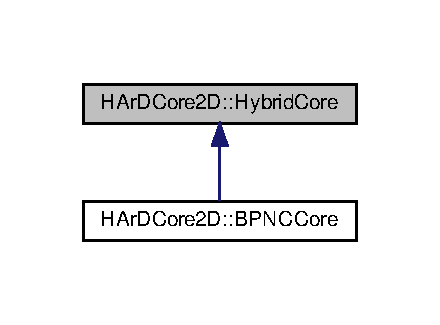
\includegraphics[width=216pt]{classHArDCore2D_1_1HybridCore__inherit__graph}
\end{center}
\end{figure}
\doxysubsection*{Public Types}
\begin{DoxyCompactItemize}
\item 
typedef \mbox{\hyperlink{classHArDCore2D_1_1Family}{Family}}$<$ \mbox{\hyperlink{classHArDCore2D_1_1MonomialScalarBasisCell}{Monomial\+Scalar\+Basis\+Cell}} $>$ \mbox{\hyperlink{group__HybridCore_ga66e8eccfa5bfc2788b2aec903bd64d4a}{Poly\+Cell\+Basis\+Type}}
\begin{DoxyCompactList}\small\item\em type for cell basis \end{DoxyCompactList}\item 
typedef \mbox{\hyperlink{classHArDCore2D_1_1Family}{Family}}$<$ \mbox{\hyperlink{classHArDCore2D_1_1MonomialScalarBasisEdge}{Monomial\+Scalar\+Basis\+Edge}} $>$ \mbox{\hyperlink{group__HybridCore_ga76550d672e82b1b9e49ea90054b8cc6d}{Poly\+Edge\+Basis\+Type}}
\begin{DoxyCompactList}\small\item\em type for edge basis \end{DoxyCompactList}\end{DoxyCompactItemize}
\doxysubsection*{Public Member Functions}
\begin{DoxyCompactItemize}
\item 
\mbox{\hyperlink{group__HybridCore_gaa13efbb29aa29dd4cf42f5881020616c}{Hybrid\+Core}} (const \mbox{\hyperlink{classHArDCore2D_1_1Mesh}{Mesh}} $\ast$mesh\+\_\+ptr, const int cell\+\_\+deg, const size\+\_\+t edge\+\_\+deg, const bool use\+\_\+threads=true, std\+::ostream \&output=std\+::cout, const bool ortho=true)
\begin{DoxyCompactList}\small\item\em Class constructor\+: initialises the data structure with the given mesh, and desired polynomial degrees of the basis functions. \end{DoxyCompactList}\item 
const \mbox{\hyperlink{classHArDCore2D_1_1Mesh}{Mesh}} $\ast$ \mbox{\hyperlink{group__HybridCore_ga8e87aec0e4162f6307eef0c04216a6cd}{get\+\_\+mesh}} () const
\begin{DoxyCompactList}\small\item\em Returns a pointer to the mesh. \end{DoxyCompactList}\item 
const int \mbox{\hyperlink{group__HybridCore_ga39e2fbe7da3ab2425544b31fab6963f1}{Cell\+Degree}} () const
\begin{DoxyCompactList}\small\item\em Return the degree of cell polynomials. \end{DoxyCompactList}\item 
const int {\bfseries Cell\+Degree\+Pos} () const
\item 
const size\+\_\+t \mbox{\hyperlink{group__HybridCore_ga58775081d94627e58f88f6043ed87bec}{Edge\+Degree}} () const
\begin{DoxyCompactList}\small\item\em Return the degree of edge polynomials. \end{DoxyCompactList}\item 
const \mbox{\hyperlink{group__HybridCore_ga66e8eccfa5bfc2788b2aec903bd64d4a}{Poly\+Cell\+Basis\+Type}} \& \mbox{\hyperlink{group__HybridCore_gafb3e4d056b781b2fff5e46466d47e0f3}{Cell\+Basis}} (size\+\_\+t iT) const
\begin{DoxyCompactList}\small\item\em Return cell basis for element with global index iT. \end{DoxyCompactList}\item 
const \mbox{\hyperlink{group__HybridCore_ga76550d672e82b1b9e49ea90054b8cc6d}{Poly\+Edge\+Basis\+Type}} \& \mbox{\hyperlink{group__HybridCore_ga9394b577ae67c9aa2289095bfedc38e2}{Edge\+Basis}} (size\+\_\+t iE) const
\begin{DoxyCompactList}\small\item\em Return edge basis for edge with global index iE. \end{DoxyCompactList}\item 
double \mbox{\hyperlink{group__HybridCore_gab37ab89bf946e237821dd978f475b7c8}{L2norm}} (const \mbox{\hyperlink{classHArDCore2D_1_1UVector}{U\+Vector}} \&Xh) const
\begin{DoxyCompactList}\small\item\em Compute L2 norm of a discrete function (using cell values) \end{DoxyCompactList}\item 
double \mbox{\hyperlink{group__HybridCore_gad6672e0691764ec5752eb1a9a7257792}{H1norm}} (const \mbox{\hyperlink{classHArDCore2D_1_1UVector}{U\+Vector}} \&Xh) const
\begin{DoxyCompactList}\small\item\em Compute discrete H1 norm of a discrete function. \end{DoxyCompactList}\item 
{\footnotesize template$<$typename Continuous\+Function $>$ }\\\mbox{\hyperlink{classHArDCore2D_1_1UVector}{U\+Vector}} \mbox{\hyperlink{group__HybridCore_ga7d6af50952aa59143ac364dd1dc4118e}{interpolate}} (const Continuous\+Function \&f, const int deg\+\_\+cell, const size\+\_\+t deg\+\_\+edge, size\+\_\+t doe) const
\begin{DoxyCompactList}\small\item\em Compute the interpolant in the discrete space of a continuous function. \end{DoxyCompactList}\item 
Eigen\+::\+Vector\+Xd \mbox{\hyperlink{group__HybridCore_ga06825c5d156026d465a2798389aa952b}{compute\+\_\+weights}} (size\+\_\+t iT) const
\begin{DoxyCompactList}\small\item\em Computes the weights to get cell values from edge values when l=-\/1. \end{DoxyCompactList}\item 
double \mbox{\hyperlink{group__HybridCore_ga9c76abf42a1d56fbf863d8258690497c}{evaluate\+\_\+in\+\_\+cell}} (const \mbox{\hyperlink{classHArDCore2D_1_1UVector}{U\+Vector}} Xh, size\+\_\+t iT, Vector\+Rd x) const
\begin{DoxyCompactList}\small\item\em Evaluates a discrete function in the cell iT at point x. \end{DoxyCompactList}\item 
double \mbox{\hyperlink{group__HybridCore_gab43816ad8a9a91f841fdb4cea0781f54}{evaluate\+\_\+in\+\_\+edge}} (const \mbox{\hyperlink{classHArDCore2D_1_1UVector}{U\+Vector}} Xh, size\+\_\+t iE, Vector\+Rd x) const
\begin{DoxyCompactList}\small\item\em Evaluates a discrete function on the edge iE at point x. \end{DoxyCompactList}\item 
Eigen\+::\+Vector\+Xd \mbox{\hyperlink{group__HybridCore_ga1d33ec0786b8127a161384ecf8f04018}{Vertex\+Values}} (const \mbox{\hyperlink{classHArDCore2D_1_1UVector}{U\+Vector}} Xh, const std\+::string from\+\_\+dofs)
\begin{DoxyCompactList}\small\item\em From a hybrid function, computes a vector of values at the vertices of the mesh. \end{DoxyCompactList}\end{DoxyCompactItemize}


\doxysubsection{Detailed Description}
The \mbox{\hyperlink{classHArDCore2D_1_1HybridCore}{Hybrid\+Core}} class provides an interface for generating polynomial basis functions on cell and edges, interpolation of continuous functions, discrete norms of vectors of coefficients, and methods to evaluate discrete functions (given by vectors of coefficients) in the cells, on the edges, or at vertices (averaged of cell or edge values)

The current implementation has the following behaviours/expectations\+:
\begin{DoxyItemize}
\item \mbox{\hyperlink{classHArDCore2D_1_1Edge}{Edge}} polynomials must be at least of degree 0, and edge basis functions are always generated
\item \mbox{\hyperlink{classHArDCore2D_1_1Cell}{Cell}} polynomials could be of degree -\/1, or 0+. In the former case, basis functions of degree 0 are generated, but a function is provided to compute weights to express the cell values in terms of linearly exact averages of edge values. This function is used, e.\+g., when interpolating a continuous function. 
\end{DoxyItemize}

The documentation for this class was generated from the following files\+:\begin{DoxyCompactItemize}
\item 
src/\+Hybrid\+Core/hybridcore.\+hpp\item 
src/\+Hybrid\+Core/hybridcore.\+cpp\end{DoxyCompactItemize}

\hypertarget{classHArDCore2D_1_1LegendreGauss}{}\section{H\+Ar\+D\+Core2D\+:\+:Legendre\+Gauss Class Reference}
\label{classHArDCore2D_1_1LegendreGauss}\index{H\+Ar\+D\+Core2\+D\+::\+Legendre\+Gauss@{H\+Ar\+D\+Core2\+D\+::\+Legendre\+Gauss}}
\subsection*{Public Member Functions}
\begin{DoxyCompactItemize}
\item 
\mbox{\Hypertarget{classHArDCore2D_1_1LegendreGauss_a4df4c78f50b0116cb68151073a45e08a}\label{classHArDCore2D_1_1LegendreGauss_a4df4c78f50b0116cb68151073a45e08a}} 
{\bfseries Legendre\+Gauss} (size\+\_\+t doe)
\item 
\mbox{\Hypertarget{classHArDCore2D_1_1LegendreGauss_aa60072df54f7acc9bad7362e4d6f6f72}\label{classHArDCore2D_1_1LegendreGauss_aa60072df54f7acc9bad7362e4d6f6f72}} 
void {\bfseries sub\+\_\+rule\+\_\+01} ()
\item 
\mbox{\Hypertarget{classHArDCore2D_1_1LegendreGauss_a3b20f2cc13f96879fe731e3411e118cf}\label{classHArDCore2D_1_1LegendreGauss_a3b20f2cc13f96879fe731e3411e118cf}} 
void {\bfseries sub\+\_\+rule\+\_\+02} ()
\item 
\mbox{\Hypertarget{classHArDCore2D_1_1LegendreGauss_a0ee58d8688bfaaa7952cd7f70e06ad05}\label{classHArDCore2D_1_1LegendreGauss_a0ee58d8688bfaaa7952cd7f70e06ad05}} 
void {\bfseries sub\+\_\+rule\+\_\+03} ()
\item 
\mbox{\Hypertarget{classHArDCore2D_1_1LegendreGauss_a55751cb4eed2cd44b12fe7bcc505097a}\label{classHArDCore2D_1_1LegendreGauss_a55751cb4eed2cd44b12fe7bcc505097a}} 
void {\bfseries sub\+\_\+rule\+\_\+04} ()
\item 
\mbox{\Hypertarget{classHArDCore2D_1_1LegendreGauss_aa4e7cbaed5cea19a7490501e67bf728b}\label{classHArDCore2D_1_1LegendreGauss_aa4e7cbaed5cea19a7490501e67bf728b}} 
void {\bfseries sub\+\_\+rule\+\_\+05} ()
\item 
\mbox{\Hypertarget{classHArDCore2D_1_1LegendreGauss_aff68078ed4cdc77372609b56c3fcfc2a}\label{classHArDCore2D_1_1LegendreGauss_aff68078ed4cdc77372609b56c3fcfc2a}} 
void {\bfseries sub\+\_\+rule\+\_\+06} ()
\item 
\mbox{\Hypertarget{classHArDCore2D_1_1LegendreGauss_a70452a921cb1f1eb6e30d7436102ae01}\label{classHArDCore2D_1_1LegendreGauss_a70452a921cb1f1eb6e30d7436102ae01}} 
void {\bfseries sub\+\_\+rule\+\_\+07} ()
\item 
\mbox{\Hypertarget{classHArDCore2D_1_1LegendreGauss_a50b4238c7cade3272efe46641e1d2d3f}\label{classHArDCore2D_1_1LegendreGauss_a50b4238c7cade3272efe46641e1d2d3f}} 
void {\bfseries sub\+\_\+rule\+\_\+08} ()
\item 
\mbox{\Hypertarget{classHArDCore2D_1_1LegendreGauss_ae6a8077dd8cf9fc76ed1234b93691049}\label{classHArDCore2D_1_1LegendreGauss_ae6a8077dd8cf9fc76ed1234b93691049}} 
void {\bfseries sub\+\_\+rule\+\_\+09} ()
\item 
\mbox{\Hypertarget{classHArDCore2D_1_1LegendreGauss_aad37934da18110fd078f1950a575fd3d}\label{classHArDCore2D_1_1LegendreGauss_aad37934da18110fd078f1950a575fd3d}} 
void {\bfseries sub\+\_\+rule\+\_\+10} ()
\item 
\mbox{\Hypertarget{classHArDCore2D_1_1LegendreGauss_a6b7095506bd1d218c28f5778c6dea545}\label{classHArDCore2D_1_1LegendreGauss_a6b7095506bd1d218c28f5778c6dea545}} 
void {\bfseries sub\+\_\+rule\+\_\+11} ()
\item 
\mbox{\Hypertarget{classHArDCore2D_1_1LegendreGauss_a1251635135ab00a28e128a058288e440}\label{classHArDCore2D_1_1LegendreGauss_a1251635135ab00a28e128a058288e440}} 
size\+\_\+t {\bfseries npts} ()
\item 
\mbox{\Hypertarget{classHArDCore2D_1_1LegendreGauss_a2800eb7a7c2648b1edb77231ef42608a}\label{classHArDCore2D_1_1LegendreGauss_a2800eb7a7c2648b1edb77231ef42608a}} 
double {\bfseries wq} (size\+\_\+t i)
\item 
\mbox{\Hypertarget{classHArDCore2D_1_1LegendreGauss_aa10e032f4ea04323773b23177b4124ee}\label{classHArDCore2D_1_1LegendreGauss_aa10e032f4ea04323773b23177b4124ee}} 
double {\bfseries tq} (size\+\_\+t i)
\end{DoxyCompactItemize}


The documentation for this class was generated from the following files\+:\begin{DoxyCompactItemize}
\item 
src/\+Quadrature/quad1d.\+hpp\item 
src/\+Quadrature/quad1d.\+cpp\end{DoxyCompactItemize}

\hypertarget{classHArDCore2D_1_1LEPNC__StefanPME}{}\doxysection{H\+Ar\+D\+Core2D\+::L\+E\+P\+N\+C\+\_\+\+Stefan\+P\+ME Class Reference}
\label{classHArDCore2D_1_1LEPNC__StefanPME}\index{HArDCore2D::LEPNC\_StefanPME@{HArDCore2D::LEPNC\_StefanPME}}


The vector Xh manipulated in the resolution has mixed components, corresponding either to the unknown u or to $\zeta(u)$, depending on the choice of weight of mass-\/lumping for the cell/edge unknowns. If no weight is put on the edges (resp. the cells), then the edge (resp. cell) unknowns represent $\zeta(u)$. Otherwise, they represent u.  




{\ttfamily \#include $<$L\+E\+P\+N\+C\+\_\+\+Stefan\+P\+M\+E.\+hpp$>$}

\doxysubsection*{Public Types}
\begin{DoxyCompactItemize}
\item 
using \mbox{\hyperlink{group__LEPNC_ga528592275ee4a7f49fcf27bb2803b38e}{solution\+\_\+function\+\_\+type}} = std\+::function$<$ double(double, double)$>$
\begin{DoxyCompactList}\small\item\em type for solution \end{DoxyCompactList}\item 
using \mbox{\hyperlink{group__LEPNC_gaa89044901a4abb21d8600c6887a6a676}{source\+\_\+function\+\_\+type}} = std\+::function$<$ double(double, double, \mbox{\hyperlink{classHArDCore2D_1_1Cell}{Cell}} $\ast$)$>$
\begin{DoxyCompactList}\small\item\em type for source \end{DoxyCompactList}\item 
using \mbox{\hyperlink{group__LEPNC_gacd93c2714bba358b33c2055e40c4aa21}{grad\+\_\+function\+\_\+type}} = std\+::function$<$ Vector\+Rd(double, double, \mbox{\hyperlink{classHArDCore2D_1_1Cell}{Cell}} $\ast$)$>$
\begin{DoxyCompactList}\small\item\em type for gradient \end{DoxyCompactList}\item 
using \mbox{\hyperlink{group__LEPNC_ga52caf522e75a28e63f86cda8cb811143}{tensor\+\_\+function\+\_\+type}} = std\+::function$<$ Eigen\+::\+Matrix2d(double, double, \mbox{\hyperlink{classHArDCore2D_1_1Cell}{Cell}} $\ast$)$>$
\begin{DoxyCompactList}\small\item\em type for diffusion tensor \end{DoxyCompactList}\end{DoxyCompactItemize}
\doxysubsection*{Public Member Functions}
\begin{DoxyCompactItemize}
\item 
\mbox{\hyperlink{group__LEPNC_ga3b61172d0528de628227d64dac41e398}{L\+E\+P\+N\+C\+\_\+\+Stefan\+P\+ME}} (\mbox{\hyperlink{classHArDCore2D_1_1LEPNCCore}{L\+E\+P\+N\+C\+Core}} \&nc, \mbox{\hyperlink{group__LEPNC_ga52caf522e75a28e63f86cda8cb811143}{tensor\+\_\+function\+\_\+type}} kappa, size\+\_\+t deg\+\_\+kappa, \mbox{\hyperlink{group__LEPNC_gaa89044901a4abb21d8600c6887a6a676}{source\+\_\+function\+\_\+type}} source, \mbox{\hyperlink{classBoundaryConditions}{Boundary\+Conditions}} BC, \mbox{\hyperlink{group__LEPNC_ga528592275ee4a7f49fcf27bb2803b38e}{solution\+\_\+function\+\_\+type}} exact\+\_\+solution, \mbox{\hyperlink{group__LEPNC_gacd93c2714bba358b33c2055e40c4aa21}{grad\+\_\+function\+\_\+type}} grad\+\_\+exact\+\_\+solution, \mbox{\hyperlink{classTestCaseNonLinearity_a3d8a5c89c517dd0d9c835b7441ee9b07}{Test\+Case\+Non\+Linearity\+::nonlinearity\+\_\+function\+\_\+type}} zeta, double weight, std\+::string solver\+\_\+type, std\+::ostream \&output=std\+::cout)
\begin{DoxyCompactList}\small\item\em Constructor of the class. \end{DoxyCompactList}\item 
Eigen\+::\+Vector\+Xd \mbox{\hyperlink{group__LEPNC_gad11f3d66f37d4811e1c58ac860f60e38}{solve}} ()
\begin{DoxyCompactList}\small\item\em Assemble and solve the scheme. \end{DoxyCompactList}\item 
Eigen\+::\+Vector\+Xd \mbox{\hyperlink{group__LEPNC_ga7a023d20d6d91ef4b3be9023ee2ae568}{apply\+\_\+nonlinearity}} (const Eigen\+::\+Vector\+Xd \&Y, const std\+::string type) const
\begin{DoxyCompactList}\small\item\em Compute non-\/linearity on vector (depends if weight=0, weight=1 or weight\textbackslash{}in (0,1) ) \end{DoxyCompactList}\item 
double \mbox{\hyperlink{group__LEPNC_ga04a4d6e8d73abdb46464e80d2a21b2e7}{L2\+\_\+\+Mass\+Lumped}} (const Eigen\+::\+Vector\+Xd Xh) const
\begin{DoxyCompactList}\small\item\em Mass-\/lumped L2 norm of a function given by a vector. \end{DoxyCompactList}\item 
double \mbox{\hyperlink{group__LEPNC_ga764da9fe2d73272eb3630f6009c992ec}{Energy\+Norm}} (const Eigen\+::\+Vector\+Xd Xh) const
\begin{DoxyCompactList}\small\item\em Discrete energy norm (associated to the diffusion operator) \end{DoxyCompactList}\item 
double \mbox{\hyperlink{group__LEPNC_ga9dc1fbcaddaa4fc0e87f1bed4d40433f}{get\+\_\+assembly\+\_\+time}} () const
\begin{DoxyCompactList}\small\item\em cpu time to assemble the scheme \end{DoxyCompactList}\item 
double \mbox{\hyperlink{group__LEPNC_gaaf712a785461b54a8070552920d674ce}{get\+\_\+solving\+\_\+time}} () const
\begin{DoxyCompactList}\small\item\em cpu time to solve the scheme \end{DoxyCompactList}\item 
double \mbox{\hyperlink{group__LEPNC_ga3747e03c1878fc65e94bcc1667f48266}{get\+\_\+solving\+\_\+error}} () const
\begin{DoxyCompactList}\small\item\em residual after solving the scheme \end{DoxyCompactList}\item 
double \mbox{\hyperlink{group__LEPNC_gaf0e776f29c97fe0ca650cd2b328caf84}{get\+\_\+itime}} (size\+\_\+t idx) const
\begin{DoxyCompactList}\small\item\em various intermediate assembly times \end{DoxyCompactList}\end{DoxyCompactItemize}


\doxysubsection{Detailed Description}
The vector Xh manipulated in the resolution has mixed components, corresponding either to the unknown u or to $\zeta(u)$, depending on the choice of weight of mass-\/lumping for the cell/edge unknowns. If no weight is put on the edges (resp. the cells), then the edge (resp. cell) unknowns represent $\zeta(u)$. Otherwise, they represent u. 

The documentation for this class was generated from the following file\+:\begin{DoxyCompactItemize}
\item 
Schemes/\+L\+E\+P\+N\+C/L\+E\+P\+N\+C\+\_\+\+Stefan\+P\+M\+E.\+hpp\end{DoxyCompactItemize}

\hypertarget{classHArDCore2D_1_1LEPNCCore}{}\doxysection{H\+Ar\+D\+Core2D\+::L\+E\+P\+N\+C\+Core Class Reference}
\label{classHArDCore2D_1_1LEPNCCore}\index{HArDCore2D::LEPNCCore@{HArDCore2D::LEPNCCore}}


{\ttfamily \#include $<$lepnccore.\+hpp$>$}



Inheritance diagram for H\+Ar\+D\+Core2D\+::L\+E\+P\+N\+C\+Core\+:
\nopagebreak
\begin{figure}[H]
\begin{center}
\leavevmode
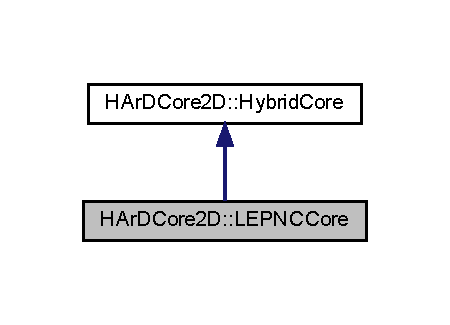
\includegraphics[width=216pt]{classHArDCore2D_1_1LEPNCCore__inherit__graph}
\end{center}
\end{figure}


Collaboration diagram for H\+Ar\+D\+Core2D\+::L\+E\+P\+N\+C\+Core\+:
\nopagebreak
\begin{figure}[H]
\begin{center}
\leavevmode
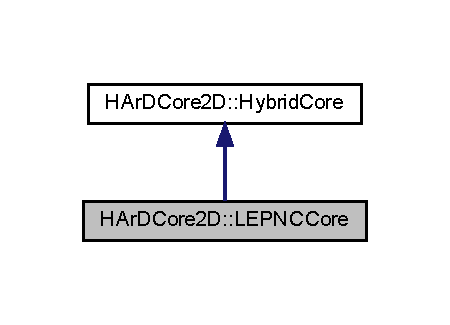
\includegraphics[width=216pt]{classHArDCore2D_1_1LEPNCCore__coll__graph}
\end{center}
\end{figure}
\doxysubsection*{Public Types}
\begin{DoxyCompactItemize}
\item 
using \mbox{\hyperlink{group__LEPNC_gaa109ebacac881c65c20a3a80cfeffba7}{cell\+\_\+basis\+\_\+type}} = std\+::function$<$ double(double, double)$>$
\begin{DoxyCompactList}\small\item\em type for cell basis \end{DoxyCompactList}\item 
using \mbox{\hyperlink{group__LEPNC_ga55bedecd14cffb98f57020923c968e89}{cell\+\_\+gradient\+\_\+type}} = std\+::function$<$ Vector\+Rd(double, double)$>$
\begin{DoxyCompactList}\small\item\em type for gradients of cell basis \end{DoxyCompactList}\end{DoxyCompactItemize}
\doxysubsection*{Public Member Functions}
\begin{DoxyCompactItemize}
\item 
\mbox{\hyperlink{group__LEPNC_ga1f6cfe8b236b45f0a1bacdfa2f266b9a}{L\+E\+P\+N\+C\+Core}} (const \mbox{\hyperlink{classHArDCore2D_1_1Mesh}{Mesh}} $\ast$mesh\+\_\+ptr, const size\+\_\+t K, const size\+\_\+t L, std\+::ostream \&output=std\+::cout)
\begin{DoxyCompactList}\small\item\em Class constructor\+: initialise the \mbox{\hyperlink{classHArDCore2D_1_1LEPNCCore}{L\+E\+P\+N\+C\+Core}} class, and creates non-\/conforming basis functions (and gradients) \end{DoxyCompactList}\item 
const \mbox{\hyperlink{group__LEPNC_gaa109ebacac881c65c20a3a80cfeffba7}{cell\+\_\+basis\+\_\+type}} \& \mbox{\hyperlink{group__LEPNC_gaccbc6dbe66d8f292e360c1f64d77d979}{nc\+\_\+basis}} (size\+\_\+t iT, size\+\_\+t i) const
\begin{DoxyCompactList}\small\item\em Return a reference to the i\textquotesingle{}th non-\/conforming basis function of the cell iT. \end{DoxyCompactList}\item 
const \mbox{\hyperlink{group__LEPNC_ga55bedecd14cffb98f57020923c968e89}{cell\+\_\+gradient\+\_\+type}} \& \mbox{\hyperlink{group__LEPNC_ga5c66560734b4c2fe07b2e21d6cd1d5a2}{nc\+\_\+gradient}} (size\+\_\+t iT, size\+\_\+t i) const
\begin{DoxyCompactList}\small\item\em Return a reference to the gradient of the i\textquotesingle{}th non-\/conforming basis function of the cell iT. \end{DoxyCompactList}\item 
const Vector\+Rd \mbox{\hyperlink{group__LEPNC_gaa71668de00ffbeccdd06b605737b0a74}{ml\+\_\+node}} (size\+\_\+t iT, size\+\_\+t i) const
\begin{DoxyCompactList}\small\item\em Return the i\textquotesingle{}th nodal point in cell iT (for mass lumping) \end{DoxyCompactList}\item 
const std\+::vector$<$ Eigen\+::\+Array\+Xd $>$ \mbox{\hyperlink{group__LEPNC_ga26cf2df3130caf5758845f5c63d9e677}{nc\+\_\+basis\+\_\+quad}} (const size\+\_\+t iT, const Quadrature\+Rule quad) const
\begin{DoxyCompactList}\small\item\em Computes non-\/conforming basis functions at the given quadrature nodes. \end{DoxyCompactList}\item 
const std\+::vector$<$ Eigen\+::\+Array\+X\+Xd $>$ \mbox{\hyperlink{group__LEPNC_ga45ee3494e636432ae9077f582c0d53c0}{grad\+\_\+nc\+\_\+basis\+\_\+quad}} (const size\+\_\+t iT, const Quadrature\+Rule quad) const
\begin{DoxyCompactList}\small\item\em Compute $(\nabla \phi_i^{nc})_{i\in I}$ at the quadrature nodes, where $(\phi_i^{nc})_{i\in I}$ are the cell basis functions. \end{DoxyCompactList}\item 
Eigen\+::\+Matrix\+Xd \mbox{\hyperlink{group__LEPNC_ga1741161cc8f8fa172bc5d5e4e2573e05}{gram\+\_\+matrix}} (const std\+::vector$<$ Eigen\+::\+Array\+Xd $>$ \&f\+\_\+quad, const std\+::vector$<$ Eigen\+::\+Array\+Xd $>$ \&g\+\_\+quad, const size\+\_\+t \&nrows, const size\+\_\+t \&ncols, const Quadrature\+Rule \&quad, const bool \&sym, std\+::vector$<$ double $>$ L2weight=\{\}) const
\item 
Eigen\+::\+Matrix\+Xd \mbox{\hyperlink{group__LEPNC_ga2cd484e7e7659ab4a73484be17a0948e}{gram\+\_\+matrix}} (const std\+::vector$<$ Eigen\+::\+Array\+X\+Xd $>$ \&F\+\_\+quad, const std\+::vector$<$ Eigen\+::\+Array\+X\+Xd $>$ \&G\+\_\+quad, const size\+\_\+t \&nrows, const size\+\_\+t \&ncols, const Quadrature\+Rule \&quad, const bool \&sym, std\+::vector$<$ Eigen\+::\+Matrix2d $>$ L2\+Weight=\{\}) const
\begin{DoxyCompactList}\small\item\em Overloaded version of the previous one for vector-\/valued functions\+: the functions (F\+\_\+i) and (G\+\_\+j) are vector-\/valued functions. \end{DoxyCompactList}\item 
{\footnotesize template$<$typename Function $>$ }\\Eigen\+::\+Vector\+Xd \mbox{\hyperlink{group__LEPNC_gac3b7abc3179ea83af2ee660c4e81f852}{nc\+\_\+interpolate\+\_\+moments}} (const Function \&f, size\+\_\+t doe) const
\begin{DoxyCompactList}\small\item\em Interpolates a continuous function on the degrees of freedom, using the moments on the basis functions. The first ones are the cell D\+O\+Fs (Dim\+Poly$<$\+Cell$>$(1) for each cell), the last ones are the edge D\+O\+Fs (one for each edge) \end{DoxyCompactList}\item 
{\footnotesize template$<$typename Function $>$ }\\Eigen\+::\+Vector\+Xd \mbox{\hyperlink{group__LEPNC_gaa86788a6f30f2a6505391795c6725834}{nc\+\_\+interpolate\+\_\+ml}} (const Function \&f, size\+\_\+t doe) const
\begin{DoxyCompactList}\small\item\em Interpolates a continuous function on the degrees of freedom, using the moments on the basis functions associated to the edges and the nodal values (corresponding to mass-\/lumping) on the cell basis functions. The first ones are the cell D\+O\+Fs (Dim\+Poly$<$\+Cell$>$(1) for each cell), the last ones are the edge D\+O\+Fs (one for each edge) \end{DoxyCompactList}\item 
Eigen\+::\+Vector\+Xd \mbox{\hyperlink{group__LEPNC_ga2b5ccb61b2dfc3b515728d77cc261d2b}{nc\+\_\+restr}} (const Eigen\+::\+Vector\+Xd \&Xh, size\+\_\+t iT) const
\begin{DoxyCompactList}\small\item\em Extract from a global vector Xh of unknowns the non-\/conforming unknowns corresponding to cell iT. \end{DoxyCompactList}\item 
double \mbox{\hyperlink{group__LEPNC_ga1c1faa68a13c6bcfa2778a35bfc5268e}{nc\+\_\+\+L2norm}} (const Eigen\+::\+Vector\+Xd \&Xh) const
\begin{DoxyCompactList}\small\item\em Compute L2 norm of a discrete function (given by coefficients on the basis functions) \end{DoxyCompactList}\item 
double \mbox{\hyperlink{group__LEPNC_gaa6e1db73269bd889a7e4311537300925}{nc\+\_\+\+L2norm\+\_\+ml}} (const Eigen\+::\+Vector\+Xd \&Xh) const
\begin{DoxyCompactList}\small\item\em Compute L2 norm of the mass-\/lumped discrete function (given by coefficients on the basis functions) \end{DoxyCompactList}\item 
double \mbox{\hyperlink{group__LEPNC_gaccf730494b67179982d6b8038e50e7fd}{nc\+\_\+\+H1norm}} (const Eigen\+::\+Vector\+Xd \&Xh) const
\begin{DoxyCompactList}\small\item\em Compute broken H1 norm of a discrete function (given by coefficients on the basis functions) \end{DoxyCompactList}\item 
double \mbox{\hyperlink{group__LEPNC_ga6594169cf850efddd4142cfa2e002994}{nc\+\_\+evaluate\+\_\+in\+\_\+cell}} (const Eigen\+::\+Vector\+Xd X\+TF, size\+\_\+t iT, double x, double y) const
\begin{DoxyCompactList}\small\item\em Evaluates a non-\/conforming discrete function in the cell iT at point (x,y) \end{DoxyCompactList}\item 
Eigen\+::\+Vector\+Xd \mbox{\hyperlink{group__LEPNC_ga138ab0f00010464e6354c22a649a4955}{nc\+\_\+\+Vertex\+Values}} (const Eigen\+::\+Vector\+Xd Xh, const double weight=0)
\begin{DoxyCompactList}\small\item\em From a non-\/conforming discrete function, computes a vector of values at the vertices of the mesh. \end{DoxyCompactList}\end{DoxyCompactItemize}


\doxysubsection{Detailed Description}
The \mbox{\hyperlink{classHArDCore2D_1_1LEPNCCore}{L\+E\+P\+N\+C\+Core}} class provides basis functions for non-\/conforming schemes on generic polygonal meshes

If using this code in a scientific publication, please cite the reference for the L\+E\+P\+NC\+:

Non-\/conforming finite elements on polytopal mesh, J. Droniou, R. Eymard, T. Gallouët and R. Herbin url\+: 

The documentation for this class was generated from the following file\+:\begin{DoxyCompactItemize}
\item 
Schemes/\+L\+E\+P\+N\+C/lepnccore.\+hpp\end{DoxyCompactItemize}

\hypertarget{classHArDCore2D_1_1Mesh}{}\doxysection{H\+Ar\+D\+Core2D\+::Mesh Class Reference}
\label{classHArDCore2D_1_1Mesh}\index{HArDCore2D::Mesh@{HArDCore2D::Mesh}}


The \mbox{\hyperlink{classHArDCore2D_1_1Mesh}{Mesh}} class provides description of a mesh.  




{\ttfamily \#include $<$mesh.\+hpp$>$}

\doxysubsection*{Public Member Functions}
\begin{DoxyCompactItemize}
\item 
\mbox{\hyperlink{group__Mesh_ga2af137f1571af89172b9c102302c416b}{Mesh}} ()
\item 
void \mbox{\hyperlink{group__Mesh_ga6ac77eb1c0d7ed0ccd8567ca03321531}{set\+\_\+name}} (std\+::string name)
\begin{DoxyCompactList}\small\item\em set the name of the mesh \end{DoxyCompactList}\item 
std\+::string \mbox{\hyperlink{group__Mesh_ga084bd89b4d3767370cbb2da9ffd8ac87}{get\+\_\+name}} ()
\begin{DoxyCompactList}\small\item\em getter for the edge name \end{DoxyCompactList}\item 
size\+\_\+t \mbox{\hyperlink{group__Mesh_ga2202a0715196c41356692d8adcfe3893}{n\+\_\+cells}} () const
\begin{DoxyCompactList}\small\item\em number of cells in the mesh \end{DoxyCompactList}\item 
size\+\_\+t \mbox{\hyperlink{group__Mesh_ga55a1cd5db98bbce8c73ab86b4527859c}{n\+\_\+edges}} () const
\begin{DoxyCompactList}\small\item\em number of edges in the mesh \end{DoxyCompactList}\item 
size\+\_\+t \mbox{\hyperlink{group__Mesh_gadb4a39bfc5444953e7799d28b8e37563}{n\+\_\+vertices}} () const
\begin{DoxyCompactList}\small\item\em number of vertices in the mesh \end{DoxyCompactList}\item 
double \mbox{\hyperlink{group__Mesh_ga5f08b04ebac390a2ab8dfe956a90ebbf}{h\+\_\+max}} () const
\begin{DoxyCompactList}\small\item\em max of diameter of cells \end{DoxyCompactList}\item 
size\+\_\+t \mbox{\hyperlink{group__Mesh_gaecd909db5f3ab863010382cf6b71ec58}{dim}} () const
\begin{DoxyCompactList}\small\item\em dimension of the mesh (2) \end{DoxyCompactList}\item 
size\+\_\+t \mbox{\hyperlink{group__Mesh_gab231e49129645ecfddafa69329c0fc51}{n\+\_\+b\+\_\+cells}} () const
\begin{DoxyCompactList}\small\item\em number of boundary cells \end{DoxyCompactList}\item 
size\+\_\+t \mbox{\hyperlink{group__Mesh_gacef44edcdc9f6d4d49d1508e7bc7ed2f}{n\+\_\+b\+\_\+edges}} () const
\begin{DoxyCompactList}\small\item\em number of boundary edges \end{DoxyCompactList}\item 
size\+\_\+t \mbox{\hyperlink{group__Mesh_ga38e8f0bf1414441ceef7e3b39526ac23}{n\+\_\+b\+\_\+vertices}} () const
\begin{DoxyCompactList}\small\item\em number of boundary vertices \end{DoxyCompactList}\item 
size\+\_\+t \mbox{\hyperlink{group__Mesh_gae31711c40d2d9888a6e8ca906bd2cbea}{n\+\_\+i\+\_\+cells}} () const
\begin{DoxyCompactList}\small\item\em number of boundary cells \end{DoxyCompactList}\item 
size\+\_\+t \mbox{\hyperlink{group__Mesh_ga7650c95dec763d4aa3fcb44644229f0e}{n\+\_\+i\+\_\+edges}} () const
\begin{DoxyCompactList}\small\item\em number of boundary edges \end{DoxyCompactList}\item 
size\+\_\+t \mbox{\hyperlink{group__Mesh_ga209126a0e22bea2f597dbc844110123c}{n\+\_\+i\+\_\+vertices}} () const
\begin{DoxyCompactList}\small\item\em number of boundary vertices \end{DoxyCompactList}\item 
std\+::vector$<$ \mbox{\hyperlink{classHArDCore2D_1_1Cell}{Cell}} $\ast$ $>$ \mbox{\hyperlink{group__Mesh_gabae9df200fe23a302b3d01e4ff13f921}{get\+\_\+cells}} () const
\begin{DoxyCompactList}\small\item\em lists the cells in the mesh. \end{DoxyCompactList}\item 
std\+::vector$<$ \mbox{\hyperlink{classHArDCore2D_1_1Edge}{Edge}} $\ast$ $>$ \mbox{\hyperlink{group__Mesh_ga9a2d7a3f9f870455465e1a9204ee3d53}{get\+\_\+edges}} () const
\begin{DoxyCompactList}\small\item\em lists the edges in the mesh. \end{DoxyCompactList}\item 
std\+::vector$<$ \mbox{\hyperlink{classHArDCore2D_1_1Vertex}{Vertex}} $\ast$ $>$ \mbox{\hyperlink{group__Mesh_ga3ef9f9e205077bdb5c1057602bde5d70}{get\+\_\+vertices}} () const
\begin{DoxyCompactList}\small\item\em lists the vertices in the mesh. \end{DoxyCompactList}\item 
\mbox{\hyperlink{classHArDCore2D_1_1Cell}{Cell}} $\ast$ \mbox{\hyperlink{group__Mesh_gae07b938c57cf57e3bb9c76d3df1eb549}{cell}} (size\+\_\+t iC) const
\begin{DoxyCompactList}\small\item\em get a constant pointer to a cell using its global index \end{DoxyCompactList}\item 
\mbox{\hyperlink{classHArDCore2D_1_1Edge}{Edge}} $\ast$ \mbox{\hyperlink{group__Mesh_gacad7cdf3d2c00fa6fc23ff77c63c7d1a}{edge}} (size\+\_\+t iE) const
\begin{DoxyCompactList}\small\item\em get a constant pointer to an edge using its global index \end{DoxyCompactList}\item 
\mbox{\hyperlink{classHArDCore2D_1_1Vertex}{Vertex}} $\ast$ \mbox{\hyperlink{group__Mesh_gad099224c697c05a57fad6a47fdcd9e76}{vertex}} (size\+\_\+t iV) const
\begin{DoxyCompactList}\small\item\em get a constant pointer to a vertex using its global index \end{DoxyCompactList}\item 
std\+::vector$<$ \mbox{\hyperlink{classHArDCore2D_1_1Cell}{Cell}} $\ast$ $>$ \mbox{\hyperlink{group__Mesh_gaf5cd4923da2e5abbe05c0f473e3b9c8f}{get\+\_\+b\+\_\+cells}} () const
\begin{DoxyCompactList}\small\item\em lists the boundary cells in the mesh. \end{DoxyCompactList}\item 
std\+::vector$<$ \mbox{\hyperlink{classHArDCore2D_1_1Edge}{Edge}} $\ast$ $>$ \mbox{\hyperlink{group__Mesh_gad876c80b23ab0c0d490b5dc8a60172b4}{get\+\_\+b\+\_\+edges}} () const
\begin{DoxyCompactList}\small\item\em lists the boundary edges in the mesh. \end{DoxyCompactList}\item 
std\+::vector$<$ \mbox{\hyperlink{classHArDCore2D_1_1Vertex}{Vertex}} $\ast$ $>$ \mbox{\hyperlink{group__Mesh_ga32dead5e72501d5001fd83aaa7379173}{get\+\_\+b\+\_\+vertices}} () const
\begin{DoxyCompactList}\small\item\em lists the boundary vertices in the mesh. \end{DoxyCompactList}\item 
\mbox{\hyperlink{classHArDCore2D_1_1Cell}{Cell}} $\ast$ \mbox{\hyperlink{group__Mesh_ga200361b60684c429e961e6b4f278dfb3}{b\+\_\+cell}} (size\+\_\+t iC) const
\begin{DoxyCompactList}\small\item\em get a constant pointer to the i\+C-\/th boundary cell \end{DoxyCompactList}\item 
\mbox{\hyperlink{classHArDCore2D_1_1Edge}{Edge}} $\ast$ \mbox{\hyperlink{group__Mesh_ga07395cbe8ecaf85abf52f91aef20422f}{b\+\_\+edge}} (size\+\_\+t iE) const
\begin{DoxyCompactList}\small\item\em get a constant pointer to the i\+E-\/th boundary edge \end{DoxyCompactList}\item 
\mbox{\hyperlink{classHArDCore2D_1_1Vertex}{Vertex}} $\ast$ \mbox{\hyperlink{group__Mesh_ga749b688ccabc6bfcf630b759607ef29a}{b\+\_\+vertex}} (size\+\_\+t iV) const
\begin{DoxyCompactList}\small\item\em get a constant pointer to the i\+V-\/th boundary vertex \end{DoxyCompactList}\item 
std\+::vector$<$ \mbox{\hyperlink{classHArDCore2D_1_1Cell}{Cell}} $\ast$ $>$ \mbox{\hyperlink{group__Mesh_gab962f4a1a88c7f4910a5e555e01064f3}{get\+\_\+i\+\_\+cells}} () const
\begin{DoxyCompactList}\small\item\em lists the interior cells in the mesh. \end{DoxyCompactList}\item 
std\+::vector$<$ \mbox{\hyperlink{classHArDCore2D_1_1Edge}{Edge}} $\ast$ $>$ \mbox{\hyperlink{group__Mesh_gabaaffe0b8981c9dab16ae34d63262638}{get\+\_\+i\+\_\+edges}} () const
\begin{DoxyCompactList}\small\item\em lists the interior edges in the mesh. \end{DoxyCompactList}\item 
std\+::vector$<$ \mbox{\hyperlink{classHArDCore2D_1_1Vertex}{Vertex}} $\ast$ $>$ \mbox{\hyperlink{group__Mesh_ga8f9f78dee50bb3c64136af58ee3468b4}{get\+\_\+i\+\_\+vertices}} () const
\begin{DoxyCompactList}\small\item\em lists the interior vertices in the mesh. \end{DoxyCompactList}\item 
\mbox{\hyperlink{classHArDCore2D_1_1Cell}{Cell}} $\ast$ \mbox{\hyperlink{group__Mesh_gaee5a30682d86cd7c130667fd4fdf395f}{i\+\_\+cell}} (size\+\_\+t iC) const
\begin{DoxyCompactList}\small\item\em get a constant pointer to the i\+C-\/th interior cell \end{DoxyCompactList}\item 
\mbox{\hyperlink{classHArDCore2D_1_1Edge}{Edge}} $\ast$ \mbox{\hyperlink{group__Mesh_gacc84a2329361880a2f821d567149a1e8}{i\+\_\+edge}} (size\+\_\+t iE) const
\begin{DoxyCompactList}\small\item\em get a constant pointer to the i\+E-\/th interior edge \end{DoxyCompactList}\item 
\mbox{\hyperlink{classHArDCore2D_1_1Vertex}{Vertex}} $\ast$ \mbox{\hyperlink{group__Mesh_ga58578f5f723f5e589ba498f74ddcbf08}{i\+\_\+vertex}} (size\+\_\+t iV) const
\begin{DoxyCompactList}\small\item\em get a constant pointer to the i\+V-\/th interior vertex \end{DoxyCompactList}\item 
bool \mbox{\hyperlink{group__Mesh_ga59082af6b1da515cdb99c4daacf5e2fd}{add\+\_\+cell}} (\mbox{\hyperlink{classHArDCore2D_1_1Cell}{Cell}} $\ast$\mbox{\hyperlink{group__Mesh_gae07b938c57cf57e3bb9c76d3df1eb549}{cell}})
\begin{DoxyCompactList}\small\item\em adds a cell to the mesh \end{DoxyCompactList}\item 
bool \mbox{\hyperlink{group__Mesh_ga9dc43dcebaa54356ddbaa45fbd94fa1a}{add\+\_\+vertex}} (\mbox{\hyperlink{classHArDCore2D_1_1Vertex}{Vertex}} $\ast$\mbox{\hyperlink{group__Mesh_gad099224c697c05a57fad6a47fdcd9e76}{vertex}})
\begin{DoxyCompactList}\small\item\em adds a vertex to the mesh \end{DoxyCompactList}\item 
\mbox{\hyperlink{classHArDCore2D_1_1Edge}{Edge}} $\ast$ \mbox{\hyperlink{group__Mesh_ga7ed3868e665ca96c2b40641524c183a1}{add\+\_\+edge}} (std\+::vector$<$ size\+\_\+t $>$ vertex\+\_\+ids, \mbox{\hyperlink{classHArDCore2D_1_1Cell}{Cell}} $\ast$\mbox{\hyperlink{group__Mesh_gae07b938c57cf57e3bb9c76d3df1eb549}{cell}})
\begin{DoxyCompactList}\small\item\em add an edge to the mesh \end{DoxyCompactList}\item 
bool \mbox{\hyperlink{group__Mesh_ga440c6f4a38af3d6c48d25fa416f24366}{add\+\_\+b\+\_\+cell}} (\mbox{\hyperlink{classHArDCore2D_1_1Cell}{Cell}} $\ast$\mbox{\hyperlink{group__Mesh_gae07b938c57cf57e3bb9c76d3df1eb549}{cell}})
\begin{DoxyCompactList}\small\item\em adds a boundary cell to the mesh \end{DoxyCompactList}\item 
bool \mbox{\hyperlink{group__Mesh_ga170b0f0bf5751a8e0cba0f5efccc66c4}{add\+\_\+b\+\_\+edge}} (\mbox{\hyperlink{classHArDCore2D_1_1Edge}{Edge}} $\ast$\mbox{\hyperlink{group__Mesh_gacad7cdf3d2c00fa6fc23ff77c63c7d1a}{edge}})
\begin{DoxyCompactList}\small\item\em adds a boundary edge to the mesh \end{DoxyCompactList}\item 
bool \mbox{\hyperlink{group__Mesh_ga75f0405bae618848b2349ebb26eec675}{add\+\_\+b\+\_\+vertex}} (\mbox{\hyperlink{classHArDCore2D_1_1Vertex}{Vertex}} $\ast$\mbox{\hyperlink{group__Mesh_gad099224c697c05a57fad6a47fdcd9e76}{vertex}})
\begin{DoxyCompactList}\small\item\em adds a boundary vertex to the mesh \end{DoxyCompactList}\item 
bool \mbox{\hyperlink{group__Mesh_ga3a47d6ebfdb4254c57b7b672b51a992b}{add\+\_\+i\+\_\+cell}} (\mbox{\hyperlink{classHArDCore2D_1_1Cell}{Cell}} $\ast$\mbox{\hyperlink{group__Mesh_gae07b938c57cf57e3bb9c76d3df1eb549}{cell}})
\begin{DoxyCompactList}\small\item\em adds an interior cell to the mesh \end{DoxyCompactList}\item 
bool \mbox{\hyperlink{group__Mesh_ga1e55100bee1027f4ab3980bf020c5df7}{add\+\_\+i\+\_\+edge}} (\mbox{\hyperlink{classHArDCore2D_1_1Edge}{Edge}} $\ast$\mbox{\hyperlink{group__Mesh_gacad7cdf3d2c00fa6fc23ff77c63c7d1a}{edge}})
\begin{DoxyCompactList}\small\item\em adds an interior edge to the mesh \end{DoxyCompactList}\item 
bool \mbox{\hyperlink{group__Mesh_gae0eac0c28f63b2106e97e595cb95248e}{add\+\_\+i\+\_\+vertex}} (\mbox{\hyperlink{classHArDCore2D_1_1Vertex}{Vertex}} $\ast$\mbox{\hyperlink{group__Mesh_gad099224c697c05a57fad6a47fdcd9e76}{vertex}})
\begin{DoxyCompactList}\small\item\em adds an interior vertex to the mesh \end{DoxyCompactList}\item 
size\+\_\+t \mbox{\hyperlink{group__Mesh_ga950e099c278cd367de1a87c6dcaefafe}{next\+\_\+edge\+\_\+idx}} ()
\begin{DoxyCompactList}\small\item\em gets the next global edge index \end{DoxyCompactList}\item 
std\+::vector$<$ double $>$ \mbox{\hyperlink{group__Mesh_ga530b237c8c966c21bdc3a16b4f266660}{regularity}} ()
\begin{DoxyCompactList}\small\item\em returns regularity factors \end{DoxyCompactList}\item 
void \mbox{\hyperlink{group__Mesh_gaf77873bbc892a7a5b37bf4773c55aefc}{renum}} (const char B, const std\+::vector$<$ size\+\_\+t $>$ new\+\_\+to\+\_\+old)
\begin{DoxyCompactList}\small\item\em Re-\/index the cells, edges or vertices. \end{DoxyCompactList}\end{DoxyCompactItemize}


\doxysubsection{Detailed Description}
The \mbox{\hyperlink{classHArDCore2D_1_1Mesh}{Mesh}} class provides description of a mesh. 

The documentation for this class was generated from the following files\+:\begin{DoxyCompactItemize}
\item 
src/\+Mesh/mesh.\+hpp\item 
src/\+Mesh/mesh.\+cpp\end{DoxyCompactItemize}

\hypertarget{classHArDCore2D_1_1MeshBuilder}{}\doxysection{H\+Ar\+D\+Core2D\+::Mesh\+Builder Class Reference}
\label{classHArDCore2D_1_1MeshBuilder}\index{HArDCore2D::MeshBuilder@{HArDCore2D::MeshBuilder}}


The \mbox{\hyperlink{classHArDCore2D_1_1MeshBuilder}{Mesh\+Builder}} class provides build tools to create a full mesh with all connectivities.  




{\ttfamily \#include $<$mesh\+\_\+builder.\+hpp$>$}

\doxysubsection*{Public Member Functions}
\begin{DoxyCompactItemize}
\item 
\mbox{\hyperlink{group__Mesh_ga13fe22fd14a85f789dc9d7d4a8d2419d}{Mesh\+Builder}} ()
\item 
\mbox{\hyperlink{group__Mesh_gafdc2fc6bdd57c06db5be137f455ab651}{Mesh\+Builder}} (const std\+::string mesh\+\_\+file)
\item 
std\+::unique\+\_\+ptr$<$ \mbox{\hyperlink{classHArDCore2D_1_1Mesh}{Mesh}} $>$ \mbox{\hyperlink{group__Mesh_ga0ef4a78ac64d1bcb6380317ea866758d}{build\+\_\+the\+\_\+mesh}} (std\+::vector$<$ std\+::vector$<$ double $>$ $>$ vertices, std\+::vector$<$ std\+::vector$<$ size\+\_\+t $>$ $>$ cells)
\begin{DoxyCompactList}\small\item\em construct the connectivity in the mesh \end{DoxyCompactList}\item 
std\+::unique\+\_\+ptr$<$ \mbox{\hyperlink{classHArDCore2D_1_1Mesh}{Mesh}} $>$ \mbox{\hyperlink{group__Mesh_ga208c94e8cb6490226215b59eb67e7911}{build\+\_\+the\+\_\+mesh}} ()
\end{DoxyCompactItemize}


\doxysubsection{Detailed Description}
The \mbox{\hyperlink{classHArDCore2D_1_1MeshBuilder}{Mesh\+Builder}} class provides build tools to create a full mesh with all connectivities. 

The documentation for this class was generated from the following files\+:\begin{DoxyCompactItemize}
\item 
src/\+Mesh/mesh\+\_\+builder.\+hpp\item 
src/\+Mesh/mesh\+\_\+builder.\+cpp\end{DoxyCompactItemize}

\hypertarget{classHArDCore2D_1_1MeshReaderTyp2}{}\section{H\+Ar\+D\+Core2D\+:\+:Mesh\+Reader\+Typ2 Class Reference}
\label{classHArDCore2D_1_1MeshReaderTyp2}\index{H\+Ar\+D\+Core2\+D\+::\+Mesh\+Reader\+Typ2@{H\+Ar\+D\+Core2\+D\+::\+Mesh\+Reader\+Typ2}}


The \hyperlink{classHArDCore2D_1_1MeshReaderTyp2}{Mesh\+Reader\+Typ2} class provides functions to read a .typ2 mesh file.  




{\ttfamily \#include $<$import\+\_\+mesh.\+hpp$>$}

\subsection*{Public Member Functions}
\begin{DoxyCompactItemize}
\item 
\hyperlink{classHArDCore2D_1_1MeshReaderTyp2_a0b4f74d0e71a0efba9699e6960d43205}{Mesh\+Reader\+Typ2} (std\+::string file\+\_\+name)
\begin{DoxyCompactList}\small\item\em class to read the cells and vertices in a .typ2 file \end{DoxyCompactList}\item 
bool \hyperlink{classHArDCore2D_1_1MeshReaderTyp2_a495a9de74127ecdf3c30c041863b9dd0}{read\+\_\+mesh} (std\+::vector$<$ std\+::vector$<$ double $>$ $>$ \&vertices, std\+::vector$<$ std\+::vector$<$ size\+\_\+t $>$ $>$ \&cells, std\+::vector$<$ std\+::vector$<$ double $>$ $>$ \&centers)
\begin{DoxyCompactList}\small\item\em reads the .typ2 file and fills in cells, vertices and centers \end{DoxyCompactList}\end{DoxyCompactItemize}


\subsection{Detailed Description}
The \hyperlink{classHArDCore2D_1_1MeshReaderTyp2}{Mesh\+Reader\+Typ2} class provides functions to read a .typ2 mesh file. 

\subsection{Constructor \& Destructor Documentation}
\mbox{\Hypertarget{classHArDCore2D_1_1MeshReaderTyp2_a0b4f74d0e71a0efba9699e6960d43205}\label{classHArDCore2D_1_1MeshReaderTyp2_a0b4f74d0e71a0efba9699e6960d43205}} 
\index{H\+Ar\+D\+Core2\+D\+::\+Mesh\+Reader\+Typ2@{H\+Ar\+D\+Core2\+D\+::\+Mesh\+Reader\+Typ2}!Mesh\+Reader\+Typ2@{Mesh\+Reader\+Typ2}}
\index{Mesh\+Reader\+Typ2@{Mesh\+Reader\+Typ2}!H\+Ar\+D\+Core2\+D\+::\+Mesh\+Reader\+Typ2@{H\+Ar\+D\+Core2\+D\+::\+Mesh\+Reader\+Typ2}}
\subsubsection{\texorpdfstring{Mesh\+Reader\+Typ2()}{MeshReaderTyp2()}}
{\footnotesize\ttfamily Mesh\+Reader\+Typ2\+::\+Mesh\+Reader\+Typ2 (\begin{DoxyParamCaption}\item[{std\+::string}]{file\+\_\+name }\end{DoxyParamCaption})}



class to read the cells and vertices in a .typ2 file 

Constructor for mesh reader


\begin{DoxyParams}{Parameters}
{\em file\+\_\+name} & name of the file name, needs to include the full path \\
\hline
\end{DoxyParams}


\subsection{Member Function Documentation}
\mbox{\Hypertarget{classHArDCore2D_1_1MeshReaderTyp2_a495a9de74127ecdf3c30c041863b9dd0}\label{classHArDCore2D_1_1MeshReaderTyp2_a495a9de74127ecdf3c30c041863b9dd0}} 
\index{H\+Ar\+D\+Core2\+D\+::\+Mesh\+Reader\+Typ2@{H\+Ar\+D\+Core2\+D\+::\+Mesh\+Reader\+Typ2}!read\+\_\+mesh@{read\+\_\+mesh}}
\index{read\+\_\+mesh@{read\+\_\+mesh}!H\+Ar\+D\+Core2\+D\+::\+Mesh\+Reader\+Typ2@{H\+Ar\+D\+Core2\+D\+::\+Mesh\+Reader\+Typ2}}
\subsubsection{\texorpdfstring{read\+\_\+mesh()}{read\_mesh()}}
{\footnotesize\ttfamily bool Mesh\+Reader\+Typ2\+::read\+\_\+mesh (\begin{DoxyParamCaption}\item[{std\+::vector$<$ std\+::vector$<$ double $>$ $>$ \&}]{vertices,  }\item[{std\+::vector$<$ std\+::vector$<$ size\+\_\+t $>$ $>$ \&}]{cells,  }\item[{std\+::vector$<$ std\+::vector$<$ double $>$ $>$ \&}]{centers }\end{DoxyParamCaption})}



reads the .typ2 file and fills in cells, vertices and centers 

Reads the file into the specified containers


\begin{DoxyParams}{Parameters}
{\em vertices} & reference to a vector to hold the vertices coordinates \\
\hline
{\em cells} & reference to a vector to hold the cell indexes \\
\hline
{\em centers} & reference to a vector to hold the cell centers coordinates \\
\hline
\end{DoxyParams}


The documentation for this class was generated from the following files\+:\begin{DoxyCompactItemize}
\item 
src/\+Mesh/import\+\_\+mesh.\+hpp\item 
src/\+Mesh/import\+\_\+mesh.\+cpp\end{DoxyCompactItemize}

\hypertarget{classHArDCore2D_1_1MonomialScalarBasisCell}{}\doxysection{H\+Ar\+D\+Core2D\+::Monomial\+Scalar\+Basis\+Cell Class Reference}
\label{classHArDCore2D_1_1MonomialScalarBasisCell}\index{HArDCore2D::MonomialScalarBasisCell@{HArDCore2D::MonomialScalarBasisCell}}


Scalar monomial basis on a cell.  




{\ttfamily \#include $<$basis.\+hpp$>$}

\doxysubsection*{Public Types}
\begin{DoxyCompactItemize}
\item 
typedef double {\bfseries Function\+Value}
\item 
typedef Vector\+Rd {\bfseries Gradient\+Value}
\item 
typedef Vector\+Rd {\bfseries Curl\+Value}
\item 
typedef double {\bfseries Divergence\+Value}
\item 
typedef \mbox{\hyperlink{classHArDCore2D_1_1Cell}{Cell}} {\bfseries Geometric\+Support}
\end{DoxyCompactItemize}
\doxysubsection*{Public Member Functions}
\begin{DoxyCompactItemize}
\item 
\mbox{\hyperlink{group__Basis_ga077d11dc2b2d74d11b72f165dc8d033a}{Monomial\+Scalar\+Basis\+Cell}} (const \mbox{\hyperlink{classHArDCore2D_1_1Cell}{Cell}} \&T, size\+\_\+t degree)
\begin{DoxyCompactList}\small\item\em Constructor. \end{DoxyCompactList}\item 
size\+\_\+t \mbox{\hyperlink{group__Basis_ga79a3220472fbc88d100be37ea1503d3e}{dimension}} () const
\begin{DoxyCompactList}\small\item\em Compute the dimension of the basis. \end{DoxyCompactList}\item 
Function\+Value \mbox{\hyperlink{group__Basis_ga82562e20ba49b9e72e04c6a7660b1d3c}{function}} (size\+\_\+t i, const Vector\+Rd \&x) const
\begin{DoxyCompactList}\small\item\em Evaluate the i-\/th basis function at point x. \end{DoxyCompactList}\item 
Gradient\+Value \mbox{\hyperlink{group__Basis_ga34784e2233789bed6214488ff9e4166d}{gradient}} (size\+\_\+t i, const Vector\+Rd \&x) const
\begin{DoxyCompactList}\small\item\em Evaluate the gradient of the i-\/th basis function at point x. \end{DoxyCompactList}\end{DoxyCompactItemize}
\doxysubsection*{Static Public Attributes}
\begin{DoxyCompactItemize}
\item 
static const Tensor\+RankE {\bfseries tensor\+Rank} = Scalar
\item 
static const bool {\bfseries has\+Function} = true
\item 
static const bool {\bfseries has\+Gradient} = true
\item 
static const bool {\bfseries has\+Curl} = false
\item 
static const bool {\bfseries has\+Divergence} = false
\end{DoxyCompactItemize}


\doxysubsection{Detailed Description}
Scalar monomial basis on a cell. 

The documentation for this class was generated from the following files\+:\begin{DoxyCompactItemize}
\item 
src/\+Common/basis.\+hpp\item 
src/\+Common/basis.\+cpp\end{DoxyCompactItemize}

\hypertarget{classHArDCore2D_1_1MonomialScalarBasisEdge}{}\doxysection{H\+Ar\+D\+Core2D\+::Monomial\+Scalar\+Basis\+Edge Class Reference}
\label{classHArDCore2D_1_1MonomialScalarBasisEdge}\index{HArDCore2D::MonomialScalarBasisEdge@{HArDCore2D::MonomialScalarBasisEdge}}


Scalar monomial basis on an edge.  




{\ttfamily \#include $<$basis.\+hpp$>$}

\doxysubsection*{Public Types}
\begin{DoxyCompactItemize}
\item 
typedef double {\bfseries Function\+Value}
\item 
typedef Vector\+Rd {\bfseries Gradient\+Value}
\item 
typedef Vector\+Rd {\bfseries Curl\+Value}
\item 
typedef double {\bfseries Divergence\+Value}
\item 
typedef \mbox{\hyperlink{classHArDCore2D_1_1Edge}{Edge}} {\bfseries Geometric\+Support}
\end{DoxyCompactItemize}
\doxysubsection*{Public Member Functions}
\begin{DoxyCompactItemize}
\item 
\mbox{\hyperlink{group__Basis_ga1794a48fbd89584ed844950e0057f513}{Monomial\+Scalar\+Basis\+Edge}} (const \mbox{\hyperlink{classHArDCore2D_1_1Edge}{Edge}} \&E, size\+\_\+t degree)
\begin{DoxyCompactList}\small\item\em Constructor. \end{DoxyCompactList}\item 
size\+\_\+t \mbox{\hyperlink{group__Basis_gae546ece15c11ddb4382aa47c50fdd53c}{dimension}} () const
\begin{DoxyCompactList}\small\item\em Dimension of the basis. \end{DoxyCompactList}\item 
Function\+Value \mbox{\hyperlink{group__Basis_gaf3ea5893997d96a77ea5a22d80777360}{function}} (size\+\_\+t i, const Vector\+Rd \&x) const
\begin{DoxyCompactList}\small\item\em Evaluate the i-\/th basis function at point x. \end{DoxyCompactList}\item 
Gradient\+Value \mbox{\hyperlink{group__Basis_ga46fbc56b645a745e1ffef6995decc5cd}{gradient}} (size\+\_\+t i, const Vector\+Rd \&x) const
\begin{DoxyCompactList}\small\item\em Evaluate the gradient of the i-\/th basis function at point x. \end{DoxyCompactList}\end{DoxyCompactItemize}
\doxysubsection*{Static Public Attributes}
\begin{DoxyCompactItemize}
\item 
static const Tensor\+RankE {\bfseries tensor\+Rank} = Scalar
\item 
static const bool {\bfseries has\+Function} = true
\item 
static const bool {\bfseries has\+Gradient} = true
\item 
static const bool {\bfseries has\+Curl} = false
\item 
static const bool {\bfseries has\+Divergence} = false
\end{DoxyCompactItemize}


\doxysubsection{Detailed Description}
Scalar monomial basis on an edge. 

The documentation for this class was generated from the following files\+:\begin{DoxyCompactItemize}
\item 
src/\+Common/basis.\+hpp\item 
src/\+Common/basis.\+cpp\end{DoxyCompactItemize}

\hypertarget{structHArDCore2D_1_1QuadratureNode}{}\doxysection{H\+Ar\+D\+Core2D\+::Quadrature\+Node Struct Reference}
\label{structHArDCore2D_1_1QuadratureNode}\index{HArDCore2D::QuadratureNode@{HArDCore2D::QuadratureNode}}


Description of one node and one weight from a quadrature rule.  




{\ttfamily \#include $<$quadraturerule.\+hpp$>$}

\doxysubsection*{Public Member Functions}
\begin{DoxyCompactItemize}
\item 
{\bfseries Quadrature\+Node} (double x, double y, double w)
\item 
Eigen\+::\+Vector2d \mbox{\hyperlink{group__Quadratures_ga27f8f3696a0be686ed1606dda2425da6}{vector}} () const
\begin{DoxyCompactList}\small\item\em Returns the quadrature point as an Eigen vector. \end{DoxyCompactList}\end{DoxyCompactItemize}
\doxysubsection*{Public Attributes}
\begin{DoxyCompactItemize}
\item 
double {\bfseries x}
\item 
double {\bfseries y}
\item 
double {\bfseries w}
\end{DoxyCompactItemize}


\doxysubsection{Detailed Description}
Description of one node and one weight from a quadrature rule. 

The documentation for this struct was generated from the following file\+:\begin{DoxyCompactItemize}
\item 
src/\+Quadrature/quadraturerule.\+hpp\end{DoxyCompactItemize}

\hypertarget{classHArDCore2D_1_1QuadRuleEdge}{}\doxysection{H\+Ar\+D\+Core2D\+::Quad\+Rule\+Edge Class Reference}
\label{classHArDCore2D_1_1QuadRuleEdge}\index{HArDCore2D::QuadRuleEdge@{HArDCore2D::QuadRuleEdge}}
\doxysubsection*{Public Member Functions}
\begin{DoxyCompactItemize}
\item 
{\bfseries Quad\+Rule\+Edge} (size\+\_\+t doe, bool warn)
\item 
size\+\_\+t {\bfseries nq} ()
\item 
double {\bfseries xq} (size\+\_\+t i)
\item 
double {\bfseries yq} (size\+\_\+t i)
\item 
double {\bfseries wq} (size\+\_\+t i)
\item 
void {\bfseries setup} (double xV\mbox{[}$\,$\mbox{]}, double yV\mbox{[}$\,$\mbox{]})
\end{DoxyCompactItemize}


The documentation for this class was generated from the following files\+:\begin{DoxyCompactItemize}
\item 
src/\+Quadrature/quad1d.\+hpp\item 
src/\+Quadrature/quad1d.\+cpp\end{DoxyCompactItemize}

\hypertarget{classHArDCore2D_1_1QuadRuleTriangle}{}\doxysection{H\+Ar\+D\+Core2D\+::Quad\+Rule\+Triangle Class Reference}
\label{classHArDCore2D_1_1QuadRuleTriangle}\index{HArDCore2D::QuadRuleTriangle@{HArDCore2D::QuadRuleTriangle}}


Wrapper for dunavant quadrature rules.  




{\ttfamily \#include $<$quad2d.\+hpp$>$}

\doxysubsection*{Public Member Functions}
\begin{DoxyCompactItemize}
\item 
\mbox{\hyperlink{classHArDCore2D_1_1QuadRuleTriangle_a83a432b56c03fffa615ec85f5dfd57d7}{Quad\+Rule\+Triangle}} (size\+\_\+t doe, bool warn)
\begin{DoxyCompactList}\small\item\em Default constructor. \end{DoxyCompactList}\item 
\mbox{\Hypertarget{classHArDCore2D_1_1QuadRuleTriangle_a5071f69f8f99171329a13943d5fe515d}\label{classHArDCore2D_1_1QuadRuleTriangle_a5071f69f8f99171329a13943d5fe515d}} 
size\+\_\+t {\bfseries nq} ()
\item 
double \mbox{\hyperlink{classHArDCore2D_1_1QuadRuleTriangle_a98156eda410a5aa6f9787ce920358fca}{xq}} (size\+\_\+t i)
\begin{DoxyCompactList}\small\item\em $<$ \end{DoxyCompactList}\item 
\mbox{\Hypertarget{classHArDCore2D_1_1QuadRuleTriangle_a0aa8f08c87bc5b2bc8180c149e16a4c2}\label{classHArDCore2D_1_1QuadRuleTriangle_a0aa8f08c87bc5b2bc8180c149e16a4c2}} 
double \mbox{\hyperlink{classHArDCore2D_1_1QuadRuleTriangle_a0aa8f08c87bc5b2bc8180c149e16a4c2}{yq}} (size\+\_\+t i)
\begin{DoxyCompactList}\small\item\em $<$ \end{DoxyCompactList}\item 
\mbox{\Hypertarget{classHArDCore2D_1_1QuadRuleTriangle_a47725c429eec36e849a8bbf69a924303}\label{classHArDCore2D_1_1QuadRuleTriangle_a47725c429eec36e849a8bbf69a924303}} 
double \mbox{\hyperlink{classHArDCore2D_1_1QuadRuleTriangle_a47725c429eec36e849a8bbf69a924303}{wq}} (size\+\_\+t i)
\begin{DoxyCompactList}\small\item\em $<$ \end{DoxyCompactList}\item 
void \mbox{\hyperlink{classHArDCore2D_1_1QuadRuleTriangle_aa2cd3081837b1cb46f6573ceb16de7b2}{setup}} (double xV\mbox{[}$\,$\mbox{]}, double yV\mbox{[}$\,$\mbox{]})
\begin{DoxyCompactList}\small\item\em $<$ \end{DoxyCompactList}\end{DoxyCompactItemize}


\doxysubsection{Detailed Description}
Wrapper for dunavant quadrature rules. 

\doxysubsection{Constructor \& Destructor Documentation}
\mbox{\Hypertarget{classHArDCore2D_1_1QuadRuleTriangle_a83a432b56c03fffa615ec85f5dfd57d7}\label{classHArDCore2D_1_1QuadRuleTriangle_a83a432b56c03fffa615ec85f5dfd57d7}} 
\index{HArDCore2D::QuadRuleTriangle@{HArDCore2D::QuadRuleTriangle}!QuadRuleTriangle@{QuadRuleTriangle}}
\index{QuadRuleTriangle@{QuadRuleTriangle}!HArDCore2D::QuadRuleTriangle@{HArDCore2D::QuadRuleTriangle}}
\doxysubsubsection{\texorpdfstring{QuadRuleTriangle()}{QuadRuleTriangle()}}
{\footnotesize\ttfamily Quad\+Rule\+Triangle\+::\+Quad\+Rule\+Triangle (\begin{DoxyParamCaption}\item[{size\+\_\+t}]{doe,  }\item[{bool}]{warn }\end{DoxyParamCaption})}



Default constructor. 


\begin{DoxyParams}{Parameters}
{\em doe} & degrees of exactness (e.\+g. how many points for approximating integral \\
\hline
{\em warn} & \\
\hline
\end{DoxyParams}


\doxysubsection{Member Function Documentation}
\mbox{\Hypertarget{classHArDCore2D_1_1QuadRuleTriangle_aa2cd3081837b1cb46f6573ceb16de7b2}\label{classHArDCore2D_1_1QuadRuleTriangle_aa2cd3081837b1cb46f6573ceb16de7b2}} 
\index{HArDCore2D::QuadRuleTriangle@{HArDCore2D::QuadRuleTriangle}!setup@{setup}}
\index{setup@{setup}!HArDCore2D::QuadRuleTriangle@{HArDCore2D::QuadRuleTriangle}}
\doxysubsubsection{\texorpdfstring{setup()}{setup()}}
{\footnotesize\ttfamily void Quad\+Rule\+Triangle\+::setup (\begin{DoxyParamCaption}\item[{double}]{xV\mbox{[}$\,$\mbox{]},  }\item[{double}]{yV\mbox{[}$\,$\mbox{]} }\end{DoxyParamCaption})}



$<$ 

get the weight for a given point \mbox{\Hypertarget{classHArDCore2D_1_1QuadRuleTriangle_a98156eda410a5aa6f9787ce920358fca}\label{classHArDCore2D_1_1QuadRuleTriangle_a98156eda410a5aa6f9787ce920358fca}} 
\index{HArDCore2D::QuadRuleTriangle@{HArDCore2D::QuadRuleTriangle}!xq@{xq}}
\index{xq@{xq}!HArDCore2D::QuadRuleTriangle@{HArDCore2D::QuadRuleTriangle}}
\doxysubsubsection{\texorpdfstring{xq()}{xq()}}
{\footnotesize\ttfamily double Quad\+Rule\+Triangle\+::xq (\begin{DoxyParamCaption}\item[{size\+\_\+t}]{i }\end{DoxyParamCaption})}



$<$ 

returns number of points 

The documentation for this class was generated from the following files\+:\begin{DoxyCompactItemize}
\item 
src/\+Quadrature/quad2d.\+hpp\item 
src/\+Quadrature/quad2d.\+cpp\end{DoxyCompactItemize}

\hypertarget{classHArDCore2D_1_1RestrictedBasis}{}\section{H\+Ar\+D\+Core2D\+:\+:Restricted\+Basis$<$ Basis\+Type $>$ Class Template Reference}
\label{classHArDCore2D_1_1RestrictedBasis}\index{H\+Ar\+D\+Core2\+D\+::\+Restricted\+Basis$<$ Basis\+Type $>$@{H\+Ar\+D\+Core2\+D\+::\+Restricted\+Basis$<$ Basis\+Type $>$}}


{\ttfamily \#include $<$basis.\+hpp$>$}

\subsection*{Public Types}
\begin{DoxyCompactItemize}
\item 
\mbox{\Hypertarget{classHArDCore2D_1_1RestrictedBasis_a5772db07ac87c68788744dc652317540}\label{classHArDCore2D_1_1RestrictedBasis_a5772db07ac87c68788744dc652317540}} 
typedef Basis\+Type\+::\+Function\+Value {\bfseries Function\+Value}
\item 
\mbox{\Hypertarget{classHArDCore2D_1_1RestrictedBasis_a2fd05335aff5beae7d23d274ccf95496}\label{classHArDCore2D_1_1RestrictedBasis_a2fd05335aff5beae7d23d274ccf95496}} 
typedef Basis\+Type\+::\+Gradient\+Value {\bfseries Gradient\+Value}
\item 
\mbox{\Hypertarget{classHArDCore2D_1_1RestrictedBasis_a76c22157064e9c58e0e45c3dfcfc8e19}\label{classHArDCore2D_1_1RestrictedBasis_a76c22157064e9c58e0e45c3dfcfc8e19}} 
typedef Vector\+Rd {\bfseries Curl\+Value}
\item 
\mbox{\Hypertarget{classHArDCore2D_1_1RestrictedBasis_a841d7df7cd3379bd3f774206dd1009d1}\label{classHArDCore2D_1_1RestrictedBasis_a841d7df7cd3379bd3f774206dd1009d1}} 
typedef double {\bfseries Divergence\+Value}
\item 
\mbox{\Hypertarget{classHArDCore2D_1_1RestrictedBasis_ac1568c98b6dcfe1198d237669218e85c}\label{classHArDCore2D_1_1RestrictedBasis_ac1568c98b6dcfe1198d237669218e85c}} 
typedef Basis\+Type\+::\+Geometric\+Support {\bfseries Geometric\+Support}
\end{DoxyCompactItemize}
\subsection*{Public Member Functions}
\begin{DoxyCompactItemize}
\item 
\hyperlink{classHArDCore2D_1_1RestrictedBasis_a3c6a0bd9f6d2d6411762613b363f1716}{Restricted\+Basis} (const Basis\+Type \&basis, const size\+\_\+t \&\hyperlink{classHArDCore2D_1_1RestrictedBasis_a5128f2da3cb58784d6ee7f4dffcacb90}{dimension})
\begin{DoxyCompactList}\small\item\em Constructor. \end{DoxyCompactList}\item 
\mbox{\Hypertarget{classHArDCore2D_1_1RestrictedBasis_a5128f2da3cb58784d6ee7f4dffcacb90}\label{classHArDCore2D_1_1RestrictedBasis_a5128f2da3cb58784d6ee7f4dffcacb90}} 
size\+\_\+t \hyperlink{classHArDCore2D_1_1RestrictedBasis_a5128f2da3cb58784d6ee7f4dffcacb90}{dimension} () const
\begin{DoxyCompactList}\small\item\em Return the dimension of the basis. \end{DoxyCompactList}\item 
\mbox{\Hypertarget{classHArDCore2D_1_1RestrictedBasis_a1d2d6afdd27878c524490c2e4a9f0bc7}\label{classHArDCore2D_1_1RestrictedBasis_a1d2d6afdd27878c524490c2e4a9f0bc7}} 
Function\+Value \hyperlink{classHArDCore2D_1_1RestrictedBasis_a1d2d6afdd27878c524490c2e4a9f0bc7}{function} (size\+\_\+t i, const Vector\+Rd \&x) const
\begin{DoxyCompactList}\small\item\em Evaluate the i-\/th basis function at point x. \end{DoxyCompactList}\item 
\mbox{\Hypertarget{classHArDCore2D_1_1RestrictedBasis_a8e3093c0bd8ca48ef8d37d8f7d302fed}\label{classHArDCore2D_1_1RestrictedBasis_a8e3093c0bd8ca48ef8d37d8f7d302fed}} 
Gradient\+Value \hyperlink{classHArDCore2D_1_1RestrictedBasis_a8e3093c0bd8ca48ef8d37d8f7d302fed}{gradient} (size\+\_\+t i, const Vector\+Rd \&x) const
\begin{DoxyCompactList}\small\item\em Evaluate the gradient of the i-\/th basis function at point x. \end{DoxyCompactList}\item 
\mbox{\Hypertarget{classHArDCore2D_1_1RestrictedBasis_a81e5a6c78223c5fe9a1e05d47a7798f1}\label{classHArDCore2D_1_1RestrictedBasis_a81e5a6c78223c5fe9a1e05d47a7798f1}} 
Curl\+Value \hyperlink{classHArDCore2D_1_1RestrictedBasis_a81e5a6c78223c5fe9a1e05d47a7798f1}{curl} (size\+\_\+t i, const Vector\+Rd \&x) const
\begin{DoxyCompactList}\small\item\em Evaluate the curl of the i-\/th basis function at point x. \end{DoxyCompactList}\item 
\mbox{\Hypertarget{classHArDCore2D_1_1RestrictedBasis_aa273301688a05d4f7e38cda0d1277212}\label{classHArDCore2D_1_1RestrictedBasis_aa273301688a05d4f7e38cda0d1277212}} 
Divergence\+Value \hyperlink{classHArDCore2D_1_1RestrictedBasis_aa273301688a05d4f7e38cda0d1277212}{divergence} (size\+\_\+t i, const Vector\+Rd \&x) const
\begin{DoxyCompactList}\small\item\em Evaluate the divergence of the i-\/th basis function at point x. \end{DoxyCompactList}\end{DoxyCompactItemize}
\subsection*{Static Public Attributes}
\begin{DoxyCompactItemize}
\item 
\mbox{\Hypertarget{classHArDCore2D_1_1RestrictedBasis_a7ac0d24bac4b90d8f97562a6f7aa5de5}\label{classHArDCore2D_1_1RestrictedBasis_a7ac0d24bac4b90d8f97562a6f7aa5de5}} 
static const Tensor\+RankE {\bfseries tensor\+Rank} = Basis\+Type\+::tensor\+Rank
\item 
\mbox{\Hypertarget{classHArDCore2D_1_1RestrictedBasis_ace08c56ba0963f5148c3ae82bc820453}\label{classHArDCore2D_1_1RestrictedBasis_ace08c56ba0963f5148c3ae82bc820453}} 
static const bool {\bfseries has\+Function} = Basis\+Type\+::has\+Function
\item 
\mbox{\Hypertarget{classHArDCore2D_1_1RestrictedBasis_a61cf97a1a52871887797bb46c15f0ba4}\label{classHArDCore2D_1_1RestrictedBasis_a61cf97a1a52871887797bb46c15f0ba4}} 
static const bool {\bfseries has\+Gradient} = Basis\+Type\+::has\+Gradient
\item 
\mbox{\Hypertarget{classHArDCore2D_1_1RestrictedBasis_a929c9098450f73e3f7f5a315ac23b1fe}\label{classHArDCore2D_1_1RestrictedBasis_a929c9098450f73e3f7f5a315ac23b1fe}} 
static const bool {\bfseries has\+Curl} = Basis\+Type\+::has\+Curl
\item 
\mbox{\Hypertarget{classHArDCore2D_1_1RestrictedBasis_a0c2322e7e67b5ca1f562db511b1e6154}\label{classHArDCore2D_1_1RestrictedBasis_a0c2322e7e67b5ca1f562db511b1e6154}} 
static const bool {\bfseries has\+Divergence} = Basis\+Type\+::has\+Divergence
\end{DoxyCompactItemize}


\subsection{Detailed Description}
\subsubsection*{template$<$typename Basis\+Type$>$\newline
class H\+Ar\+D\+Core2\+D\+::\+Restricted\+Basis$<$ Basis\+Type $>$}

Generate a basis restricted to the first \char`\"{}dimension\char`\"{} functions. This can be useful, e.\+g., to form bases of subspaces of a given space from a hierarchical basis of the latter 

\subsection{Constructor \& Destructor Documentation}
\mbox{\Hypertarget{classHArDCore2D_1_1RestrictedBasis_a3c6a0bd9f6d2d6411762613b363f1716}\label{classHArDCore2D_1_1RestrictedBasis_a3c6a0bd9f6d2d6411762613b363f1716}} 
\index{H\+Ar\+D\+Core2\+D\+::\+Restricted\+Basis@{H\+Ar\+D\+Core2\+D\+::\+Restricted\+Basis}!Restricted\+Basis@{Restricted\+Basis}}
\index{Restricted\+Basis@{Restricted\+Basis}!H\+Ar\+D\+Core2\+D\+::\+Restricted\+Basis@{H\+Ar\+D\+Core2\+D\+::\+Restricted\+Basis}}
\subsubsection{\texorpdfstring{Restricted\+Basis()}{RestrictedBasis()}}
{\footnotesize\ttfamily template$<$typename Basis\+Type $>$ \\
\hyperlink{classHArDCore2D_1_1RestrictedBasis}{H\+Ar\+D\+Core2\+D\+::\+Restricted\+Basis}$<$ Basis\+Type $>$\+::\hyperlink{classHArDCore2D_1_1RestrictedBasis}{Restricted\+Basis} (\begin{DoxyParamCaption}\item[{const Basis\+Type \&}]{basis,  }\item[{const size\+\_\+t \&}]{dimension }\end{DoxyParamCaption})\hspace{0.3cm}{\ttfamily [inline]}}



Constructor. 


\begin{DoxyParams}{Parameters}
{\em basis} & A basis \\
\hline
{\em dimension} & The dimension of the restricted basis \\
\hline
\end{DoxyParams}


The documentation for this class was generated from the following file\+:\begin{DoxyCompactItemize}
\item 
src/\+Common/basis.\+hpp\end{DoxyCompactItemize}

\hypertarget{classHArDCore2D_1_1ShiftedBasis}{}\doxysection{H\+Ar\+D\+Core2D\+::Shifted\+Basis$<$ Basis\+Type $>$ Class Template Reference}
\label{classHArDCore2D_1_1ShiftedBasis}\index{HArDCore2D::ShiftedBasis$<$ BasisType $>$@{HArDCore2D::ShiftedBasis$<$ BasisType $>$}}


{\ttfamily \#include $<$basis.\+hpp$>$}

\doxysubsection*{Public Types}
\begin{DoxyCompactItemize}
\item 
typedef Basis\+Type\+::\+Function\+Value {\bfseries Function\+Value}
\item 
typedef Basis\+Type\+::\+Gradient\+Value {\bfseries Gradient\+Value}
\item 
typedef Vector\+Rd {\bfseries Curl\+Value}
\item 
typedef double {\bfseries Divergence\+Value}
\item 
typedef Basis\+Type\+::\+Geometric\+Support {\bfseries Geometric\+Support}
\end{DoxyCompactItemize}
\doxysubsection*{Public Member Functions}
\begin{DoxyCompactItemize}
\item 
\mbox{\hyperlink{group__Basis_gadb935c3f74623dbd29c124c0c6dc605e}{Shifted\+Basis}} (const Basis\+Type \&basis, const int shift)
\begin{DoxyCompactList}\small\item\em Constructor. \end{DoxyCompactList}\item 
size\+\_\+t \mbox{\hyperlink{group__Basis_ga74ebe98de6bd42447c4743c784e8c601}{dimension}} () const
\begin{DoxyCompactList}\small\item\em Return the dimension of the basis. \end{DoxyCompactList}\item 
Function\+Value \mbox{\hyperlink{group__Basis_ga73529b85e8d087fdeee582e0744bf49a}{function}} (size\+\_\+t i, const Vector\+Rd \&x) const
\begin{DoxyCompactList}\small\item\em Evaluate the i-\/th basis function at point x. \end{DoxyCompactList}\item 
Gradient\+Value \mbox{\hyperlink{group__Basis_ga7c06ac1c5648d70651308067df98c4c8}{gradient}} (size\+\_\+t i, const Vector\+Rd \&x) const
\begin{DoxyCompactList}\small\item\em Evaluate the gradient of the i-\/th basis function at point x. \end{DoxyCompactList}\item 
Curl\+Value \mbox{\hyperlink{group__Basis_ga7cb372f9d9384f30cecd1beb4b5d62b7}{curl}} (size\+\_\+t i, const Vector\+Rd \&x) const
\begin{DoxyCompactList}\small\item\em Evaluate the curl of the i-\/th basis function at point x. \end{DoxyCompactList}\item 
Divergence\+Value \mbox{\hyperlink{group__Basis_ga84d8719be3260330c3c2e80dbf1b4eed}{divergence}} (size\+\_\+t i, const Vector\+Rd \&x) const
\begin{DoxyCompactList}\small\item\em Evaluate the divergence of the i-\/th basis function at point x. \end{DoxyCompactList}\end{DoxyCompactItemize}
\doxysubsection*{Static Public Attributes}
\begin{DoxyCompactItemize}
\item 
static const Tensor\+RankE {\bfseries tensor\+Rank} = Basis\+Type\+::tensor\+Rank
\item 
static const bool {\bfseries has\+Function} = Basis\+Type\+::has\+Function
\item 
static const bool {\bfseries has\+Gradient} = Basis\+Type\+::has\+Gradient
\item 
static const bool {\bfseries has\+Curl} = Basis\+Type\+::has\+Curl
\item 
static const bool {\bfseries has\+Divergence} = Basis\+Type\+::has\+Divergence
\end{DoxyCompactItemize}


\doxysubsection{Detailed Description}
\subsubsection*{template$<$typename Basis\+Type$>$\newline
class H\+Ar\+D\+Core2\+D\+::\+Shifted\+Basis$<$ Basis\+Type $>$}

Generate a basis where the function indices are shifted. Can be used, e.\+g., to ignore the constant function in scalar bases 

The documentation for this class was generated from the following file\+:\begin{DoxyCompactItemize}
\item 
src/\+Common/basis.\+hpp\end{DoxyCompactItemize}

\hypertarget{classHArDCore2D_1_1TensorizedVectorFamily}{}\section{H\+Ar\+D\+Core2D\+:\+:Tensorized\+Vector\+Family$<$ Scalar\+Family\+Type, N $>$ Class Template Reference}
\label{classHArDCore2D_1_1TensorizedVectorFamily}\index{H\+Ar\+D\+Core2\+D\+::\+Tensorized\+Vector\+Family$<$ Scalar\+Family\+Type, N $>$@{H\+Ar\+D\+Core2\+D\+::\+Tensorized\+Vector\+Family$<$ Scalar\+Family\+Type, N $>$}}


{\ttfamily \#include $<$basis.\+hpp$>$}

\subsection*{Public Types}
\begin{DoxyCompactItemize}
\item 
\mbox{\Hypertarget{classHArDCore2D_1_1TensorizedVectorFamily_a55ec3e0805c4dd4a6758a94d04924520}\label{classHArDCore2D_1_1TensorizedVectorFamily_a55ec3e0805c4dd4a6758a94d04924520}} 
typedef Eigen\+::\+Matrix$<$ double, N, 1 $>$ {\bfseries Function\+Value}
\item 
\mbox{\Hypertarget{classHArDCore2D_1_1TensorizedVectorFamily_a03e55037df352b512c181687d4526b11}\label{classHArDCore2D_1_1TensorizedVectorFamily_a03e55037df352b512c181687d4526b11}} 
typedef Eigen\+::\+Matrix$<$ double, N, dimspace $>$ {\bfseries Gradient\+Value}
\item 
\mbox{\Hypertarget{classHArDCore2D_1_1TensorizedVectorFamily_a88c7890d4b589d1e2cbe582445e638bb}\label{classHArDCore2D_1_1TensorizedVectorFamily_a88c7890d4b589d1e2cbe582445e638bb}} 
typedef Vector\+Rd {\bfseries Curl\+Value}
\item 
\mbox{\Hypertarget{classHArDCore2D_1_1TensorizedVectorFamily_ab1dda1064d631768943c7658d2e69edd}\label{classHArDCore2D_1_1TensorizedVectorFamily_ab1dda1064d631768943c7658d2e69edd}} 
typedef double {\bfseries Divergence\+Value}
\item 
\mbox{\Hypertarget{classHArDCore2D_1_1TensorizedVectorFamily_ad1c8c80da131a654a1a91a43e379cc57}\label{classHArDCore2D_1_1TensorizedVectorFamily_ad1c8c80da131a654a1a91a43e379cc57}} 
typedef Scalar\+Family\+Type\+::\+Geometric\+Support {\bfseries Geometric\+Support}
\end{DoxyCompactItemize}
\subsection*{Public Member Functions}
\begin{DoxyCompactItemize}
\item 
\mbox{\Hypertarget{classHArDCore2D_1_1TensorizedVectorFamily_afbbde5d4b671418870cbbd903a0a409b}\label{classHArDCore2D_1_1TensorizedVectorFamily_afbbde5d4b671418870cbbd903a0a409b}} 
{\bfseries Tensorized\+Vector\+Family} (const Scalar\+Family\+Type \&scalar\+\_\+family)
\item 
\mbox{\Hypertarget{classHArDCore2D_1_1TensorizedVectorFamily_abdcbe0043887c0aa46065409f1731a83}\label{classHArDCore2D_1_1TensorizedVectorFamily_abdcbe0043887c0aa46065409f1731a83}} 
size\+\_\+t \hyperlink{classHArDCore2D_1_1TensorizedVectorFamily_abdcbe0043887c0aa46065409f1731a83}{dimension} () const
\begin{DoxyCompactList}\small\item\em Return the dimension of the family. \end{DoxyCompactList}\item 
\mbox{\Hypertarget{classHArDCore2D_1_1TensorizedVectorFamily_a52d9aaac677abb3a81b32c5542e55ea4}\label{classHArDCore2D_1_1TensorizedVectorFamily_a52d9aaac677abb3a81b32c5542e55ea4}} 
Function\+Value \hyperlink{classHArDCore2D_1_1TensorizedVectorFamily_a52d9aaac677abb3a81b32c5542e55ea4}{function} (size\+\_\+t i, const Vector\+Rd \&x) const
\begin{DoxyCompactList}\small\item\em Evaluate the i-\/th basis function at point x. \end{DoxyCompactList}\item 
\mbox{\Hypertarget{classHArDCore2D_1_1TensorizedVectorFamily_a46500da07e2cb4cfe8ead5ffe8dbc586}\label{classHArDCore2D_1_1TensorizedVectorFamily_a46500da07e2cb4cfe8ead5ffe8dbc586}} 
Gradient\+Value \hyperlink{classHArDCore2D_1_1TensorizedVectorFamily_a46500da07e2cb4cfe8ead5ffe8dbc586}{gradient} (size\+\_\+t i, const Vector\+Rd \&x) const
\begin{DoxyCompactList}\small\item\em Evaluate the gradient of the i-\/th basis function at point x. \end{DoxyCompactList}\item 
\mbox{\Hypertarget{classHArDCore2D_1_1TensorizedVectorFamily_a187befd7daa85ec049e41706ea1d5de2}\label{classHArDCore2D_1_1TensorizedVectorFamily_a187befd7daa85ec049e41706ea1d5de2}} 
Curl\+Value \hyperlink{classHArDCore2D_1_1TensorizedVectorFamily_a187befd7daa85ec049e41706ea1d5de2}{curl} (size\+\_\+t i, const Vector\+Rd \&x) const
\begin{DoxyCompactList}\small\item\em Evaluate the curl of the i-\/th basis function at point x. \end{DoxyCompactList}\item 
\mbox{\Hypertarget{classHArDCore2D_1_1TensorizedVectorFamily_a6e852fda44755e4ca0a8ffac94d97d16}\label{classHArDCore2D_1_1TensorizedVectorFamily_a6e852fda44755e4ca0a8ffac94d97d16}} 
Divergence\+Value \hyperlink{classHArDCore2D_1_1TensorizedVectorFamily_a6e852fda44755e4ca0a8ffac94d97d16}{divergence} (size\+\_\+t i, const Vector\+Rd \&x) const
\begin{DoxyCompactList}\small\item\em Evaluate the divergence of the i-\/th basis function at point x. \end{DoxyCompactList}\end{DoxyCompactItemize}
\subsection*{Static Public Attributes}
\begin{DoxyCompactItemize}
\item 
\mbox{\Hypertarget{classHArDCore2D_1_1TensorizedVectorFamily_aada1d8a90047badc9910b9b312e6300e}\label{classHArDCore2D_1_1TensorizedVectorFamily_aada1d8a90047badc9910b9b312e6300e}} 
static const Tensor\+RankE {\bfseries tensor\+Rank} = Vector
\item 
\mbox{\Hypertarget{classHArDCore2D_1_1TensorizedVectorFamily_a11bea467eab12156126ffc5d296ffecc}\label{classHArDCore2D_1_1TensorizedVectorFamily_a11bea467eab12156126ffc5d296ffecc}} 
static const bool {\bfseries has\+Function} = Scalar\+Family\+Type\+::has\+Function
\item 
\mbox{\Hypertarget{classHArDCore2D_1_1TensorizedVectorFamily_a118c8e9bbbe5d63d2ce9575adf4e02eb}\label{classHArDCore2D_1_1TensorizedVectorFamily_a118c8e9bbbe5d63d2ce9575adf4e02eb}} 
static const bool {\bfseries has\+Gradient} = Scalar\+Family\+Type\+::has\+Gradient
\item 
\mbox{\Hypertarget{classHArDCore2D_1_1TensorizedVectorFamily_a67fc626998e10c80c40b9419e013e538}\label{classHArDCore2D_1_1TensorizedVectorFamily_a67fc626998e10c80c40b9419e013e538}} 
static const bool {\bfseries has\+Divergence} = ( Scalar\+Family\+Type\+::has\+Gradient \&\& N==dimspace )
\item 
\mbox{\Hypertarget{classHArDCore2D_1_1TensorizedVectorFamily_a440a12913a7f63653b9766e4180c5884}\label{classHArDCore2D_1_1TensorizedVectorFamily_a440a12913a7f63653b9766e4180c5884}} 
static const bool {\bfseries has\+Curl} = ( Scalar\+Family\+Type\+::has\+Gradient \&\& N==dimspace )
\end{DoxyCompactItemize}


\subsection{Detailed Description}
\subsubsection*{template$<$typename Scalar\+Family\+Type, size\+\_\+t N$>$\newline
class H\+Ar\+D\+Core2\+D\+::\+Tensorized\+Vector\+Family$<$ Scalar\+Family\+Type, N $>$}

Vector family obtained by tensorization of a scalar family The tensorization is done the following way\+: if (f\+\_\+1,...,f\+\_\+r) is the family of scalar functions, the tensorized family of rank N is given by (where all vectors are columns of size N)\+:

$\left(\begin{array}{c}f_1\\0\\\vdots\\0\end{array}\right)$; $\left(\begin{array}{c}f_2\\0\\\vdots\\0\end{array}\right)$;...; $\left(\begin{array}{c}f_r\\0\\\vdots\\0\end{array}\right)$; $\left(\begin{array}{c}0\\f_1\\0\\\vdots\\0\end{array}\right)$; $\left(\begin{array}{c}0\\f_2\\0\\\vdots\\0\end{array}\right)$;...; $\left(\begin{array}{c}0\\f_r\\0\\\vdots\\0\end{array}\right)$;...; $\left(\begin{array}{c}0\\\vdots\\0\\f_1\end{array}\right)$;...; $\left(\begin{array}{c}0\\\vdots\\0\\f_r\end{array}\right)$

The gradient values are therefore matrices of size N$\ast$r, where the gradients of the scalar functions are put in rows\+:

$\left(\begin{array}{c}(\nabla f_1)^t\\0\\\vdots\\0\end{array}\right)$; $\left(\begin{array}{c}(\nabla f_2)^t\\0\\\vdots\\0\end{array}\right)$;...; $\left(\begin{array}{c}(\nabla f_r)^t\\0\\\vdots\\0\end{array}\right)$; $\left(\begin{array}{c}0\\(\nabla f_1)^t\\0\\\vdots\\0\end{array}\right)$; $\left(\begin{array}{c}0\\(\nabla f_2)^t\\0\\\vdots\\0\end{array}\right)$;...; $\left(\begin{array}{c}0\\(\nabla f_r)^t\\0\\\vdots\\0\end{array}\right)$;...; $\left(\begin{array}{c}0\\\vdots\\0\\(\nabla f_1)^t\end{array}\right)$;...; $\left(\begin{array}{c}0\\\vdots\\0\\(\nabla f_r)^t\end{array}\right)$ 

The documentation for this class was generated from the following file\+:\begin{DoxyCompactItemize}
\item 
src/\+Common/basis.\+hpp\end{DoxyCompactItemize}

\hypertarget{classTestCase}{}\section{Test\+Case Class Reference}
\label{classTestCase}\index{Test\+Case@{Test\+Case}}


The \hyperlink{classTestCase}{Test\+Case} class provides definition of test cases.  




{\ttfamily \#include $<$Test\+Case.\+hpp$>$}

\subsection*{Public Member Functions}
\begin{DoxyCompactItemize}
\item 
\hyperlink{classTestCase_aa4ad29533416ee515205db87002a1bf1}{Test\+Case} (const std\+::vector$<$ int $>$ i\+TC)
\begin{DoxyCompactList}\small\item\em Initialise data. \end{DoxyCompactList}\item 
double \hyperlink{classTestCase_aede719dac81c460c713d930a379c537e}{sol} (const double x, const double y)
\begin{DoxyCompactList}\small\item\em Returns the exact solution at the points x, y. \end{DoxyCompactList}\item 
Eigen\+::\+Vector2d \hyperlink{classTestCase_a2e3004705b74b232dc54d84652ec88ae}{grad\+\_\+sol} (const double x, const double y, const \hyperlink{classHArDCore2D_1_1Cell}{Cell} $\ast$cell)
\begin{DoxyCompactList}\small\item\em Returns the gradient of the exact solution at the points x, y. \end{DoxyCompactList}\item 
Eigen\+::\+Matrix2d \hyperlink{classTestCase_aadf1375364b34ad3b9fa651eae5baa1e}{hess\+\_\+sol} (const double x, const double y, const \hyperlink{classHArDCore2D_1_1Cell}{Cell} $\ast$cell)
\begin{DoxyCompactList}\small\item\em Returns the Hessian of the exact solution at the points x, y. \end{DoxyCompactList}\item 
Eigen\+::\+Matrix2d \hyperlink{classTestCase_aaf745f4815ce0e9c16d8bded9f9b3596}{diff} (const double x, const double y, const \hyperlink{classHArDCore2D_1_1Cell}{Cell} $\ast$cell)
\begin{DoxyCompactList}\small\item\em Returns the diffusion matrix at the points x, y. \end{DoxyCompactList}\item 
Eigen\+::\+Vector2d \hyperlink{classTestCase_aa32221ff5dd860c050a28661406a87dc}{div\+\_\+diff} (const double x, const double y, const \hyperlink{classHArDCore2D_1_1Cell}{Cell} $\ast$cell)
\begin{DoxyCompactList}\small\item\em Returns the divergence by row of the diffusion matrix at the points x, y. \end{DoxyCompactList}\item 
double \hyperlink{classTestCase_a5b2e54e9f17ac2ec9c1d675f97fbe335}{source} (const double x, const double y, const \hyperlink{classHArDCore2D_1_1Cell}{Cell} $\ast$cell)
\begin{DoxyCompactList}\small\item\em Returns the source term at the points x, y. \end{DoxyCompactList}\item 
double \hyperlink{group__TestCases_gabb42d3b206c5e89d34ed34f5fe2546e0}{get\+\_\+lambda} ()
\begin{DoxyCompactList}\small\item\em Returns the value of the parameter lambda. \end{DoxyCompactList}\item 
\mbox{\Hypertarget{classTestCase_a1f428652eb476f6eb4973ef1f478e8ce}\label{classTestCase_a1f428652eb476f6eb4973ef1f478e8ce}} 
void \hyperlink{classTestCase_a1f428652eb476f6eb4973ef1f478e8ce}{validate} ()
\begin{DoxyCompactList}\small\item\em Check if the provided test cases are valid (within range, and combination of solution/diffusion valid) \end{DoxyCompactList}\item 
size\+\_\+t \hyperlink{group__TestCases_ga3dd2daaebb012281b252ab65db0045b2}{get\+\_\+deg\+\_\+diff} ()
\begin{DoxyCompactList}\small\item\em Returns the degree of the diffusion tensor (useful to set up quadrature rules of proper degree) \end{DoxyCompactList}\end{DoxyCompactItemize}


\subsection{Detailed Description}
The \hyperlink{classTestCase}{Test\+Case} class provides definition of test cases. 

\subsection{Constructor \& Destructor Documentation}
\mbox{\Hypertarget{classTestCase_aa4ad29533416ee515205db87002a1bf1}\label{classTestCase_aa4ad29533416ee515205db87002a1bf1}} 
\index{Test\+Case@{Test\+Case}!Test\+Case@{Test\+Case}}
\index{Test\+Case@{Test\+Case}!Test\+Case@{Test\+Case}}
\subsubsection{\texorpdfstring{Test\+Case()}{TestCase()}}
{\footnotesize\ttfamily Test\+Case\+::\+Test\+Case (\begin{DoxyParamCaption}\item[{const std\+::vector$<$ int $>$}]{i\+TC }\end{DoxyParamCaption})}



Initialise data. 


\begin{DoxyParams}{Parameters}
{\em i\+TC} & The vector id of the test case\+: (id of solution, id of diffusion) \\
\hline
\end{DoxyParams}


\subsection{Member Function Documentation}
\mbox{\Hypertarget{classTestCase_aaf745f4815ce0e9c16d8bded9f9b3596}\label{classTestCase_aaf745f4815ce0e9c16d8bded9f9b3596}} 
\index{Test\+Case@{Test\+Case}!diff@{diff}}
\index{diff@{diff}!Test\+Case@{Test\+Case}}
\subsubsection{\texorpdfstring{diff()}{diff()}}
{\footnotesize\ttfamily Eigen\+::\+Matrix2d Test\+Case\+::diff (\begin{DoxyParamCaption}\item[{const double}]{x,  }\item[{const double}]{y,  }\item[{const \hyperlink{classHArDCore2D_1_1Cell}{Cell} $\ast$}]{cell }\end{DoxyParamCaption})}



Returns the diffusion matrix at the points x, y. 

i\+TC\mbox{[}1\mbox{]}=1\+: Diff = Id

i\+TC\mbox{[}1\mbox{]}=2\+: Diff = $\left[\begin{array}{cc}y^2+1 & -xy\\ -xy & x^2+1\end{array}\right]$

i\+TC\mbox{[}1\mbox{]}=3\+: Diff= $\left[\begin{array}{cc}\lambda & 0\\ 0 & 1\end{array}\right]$ if $y<1/2$, Diff=Id if $y\ge 1/2$. Only valid with i\+TC\mbox{[}0\mbox{]}=2 ( $\partial_x u$ must vanish along $y=1/2$).

i\+TC\mbox{[}1\mbox{]}=4\+: rotating diffusion. Diff= $\left[\begin{array}{cc}\epsilon \bar{x}^2 + \bar{y}^2 & (\epsilon-1)\bar{x}\bar{y}\\ (\epsilon-1)\bar{x}\bar{y} & \bar{x}^2+\epsilon \bar{y}^2\end{array}\right]$, where $\bar{x}=x+0.1$ and $\bar{y}=y+0.1$.

i\+TC\mbox{[}1\mbox{]}=5\+: Diff= $\left[\begin{array}{cc}\lambda & 0\\ 0 & 1\end{array}\right]$. 
\begin{DoxyParams}{Parameters}
{\em cell} & In case of discontinuity, we need to know the cell we\textquotesingle{}re in to select the correct formula \\
\hline
\end{DoxyParams}
\mbox{\Hypertarget{classTestCase_aa32221ff5dd860c050a28661406a87dc}\label{classTestCase_aa32221ff5dd860c050a28661406a87dc}} 
\index{Test\+Case@{Test\+Case}!div\+\_\+diff@{div\+\_\+diff}}
\index{div\+\_\+diff@{div\+\_\+diff}!Test\+Case@{Test\+Case}}
\subsubsection{\texorpdfstring{div\+\_\+diff()}{div\_diff()}}
{\footnotesize\ttfamily Eigen\+::\+Vector2d Test\+Case\+::div\+\_\+diff (\begin{DoxyParamCaption}\item[{const double}]{x,  }\item[{const double}]{y,  }\item[{const \hyperlink{classHArDCore2D_1_1Cell}{Cell} $\ast$}]{cell }\end{DoxyParamCaption})}



Returns the divergence by row of the diffusion matrix at the points x, y. 


\begin{DoxyParams}{Parameters}
{\em cell} & In case of discontinuity, we need to know the cell we\textquotesingle{}re in to select the correct formula \\
\hline
\end{DoxyParams}
\mbox{\Hypertarget{classTestCase_a2e3004705b74b232dc54d84652ec88ae}\label{classTestCase_a2e3004705b74b232dc54d84652ec88ae}} 
\index{Test\+Case@{Test\+Case}!grad\+\_\+sol@{grad\+\_\+sol}}
\index{grad\+\_\+sol@{grad\+\_\+sol}!Test\+Case@{Test\+Case}}
\subsubsection{\texorpdfstring{grad\+\_\+sol()}{grad\_sol()}}
{\footnotesize\ttfamily Eigen\+::\+Vector2d Test\+Case\+::grad\+\_\+sol (\begin{DoxyParamCaption}\item[{const double}]{x,  }\item[{const double}]{y,  }\item[{const \hyperlink{classHArDCore2D_1_1Cell}{Cell} $\ast$}]{cell }\end{DoxyParamCaption})}



Returns the gradient of the exact solution at the points x, y. 


\begin{DoxyParams}{Parameters}
{\em cell} & In case of discontinuity, we need to know the cell we\textquotesingle{}re in to select the correct formula \\
\hline
\end{DoxyParams}
\mbox{\Hypertarget{classTestCase_aadf1375364b34ad3b9fa651eae5baa1e}\label{classTestCase_aadf1375364b34ad3b9fa651eae5baa1e}} 
\index{Test\+Case@{Test\+Case}!hess\+\_\+sol@{hess\+\_\+sol}}
\index{hess\+\_\+sol@{hess\+\_\+sol}!Test\+Case@{Test\+Case}}
\subsubsection{\texorpdfstring{hess\+\_\+sol()}{hess\_sol()}}
{\footnotesize\ttfamily Eigen\+::\+Matrix2d Test\+Case\+::hess\+\_\+sol (\begin{DoxyParamCaption}\item[{const double}]{x,  }\item[{const double}]{y,  }\item[{const \hyperlink{classHArDCore2D_1_1Cell}{Cell} $\ast$}]{cell }\end{DoxyParamCaption})}



Returns the Hessian of the exact solution at the points x, y. 


\begin{DoxyParams}{Parameters}
{\em cell} & In case of discontinuity, we need to know the cell we\textquotesingle{}re in to select the correct formula \\
\hline
\end{DoxyParams}
\mbox{\Hypertarget{classTestCase_aede719dac81c460c713d930a379c537e}\label{classTestCase_aede719dac81c460c713d930a379c537e}} 
\index{Test\+Case@{Test\+Case}!sol@{sol}}
\index{sol@{sol}!Test\+Case@{Test\+Case}}
\subsubsection{\texorpdfstring{sol()}{sol()}}
{\footnotesize\ttfamily double Test\+Case\+::sol (\begin{DoxyParamCaption}\item[{const double}]{x,  }\item[{const double}]{y }\end{DoxyParamCaption})}



Returns the exact solution at the points x, y. 

i\+TC\mbox{[}0\mbox{]}=1\+: $u(x,y)=sin(\pi x) sin(\pi y)$

i\+TC\mbox{[}0\mbox{]}=2\+: $u(x,y)=cos(\pi x) cos(\pi y)$

i\+TC\mbox{[}0\mbox{]}=3\+: $u(x,y)= x$

i\+TC\mbox{[}0\mbox{]}=4\+: $u(x,y)= y$

i\+TC\mbox{[}0\mbox{]}=5\+: $u(x,y)= x^2 + y^2$

i\+TC\mbox{[}0\mbox{]}=6\+: $u(x,y)= e^x \sin(pi x) \cos(\pi x)$ \mbox{\Hypertarget{classTestCase_a5b2e54e9f17ac2ec9c1d675f97fbe335}\label{classTestCase_a5b2e54e9f17ac2ec9c1d675f97fbe335}} 
\index{Test\+Case@{Test\+Case}!source@{source}}
\index{source@{source}!Test\+Case@{Test\+Case}}
\subsubsection{\texorpdfstring{source()}{source()}}
{\footnotesize\ttfamily double Test\+Case\+::source (\begin{DoxyParamCaption}\item[{const double}]{x,  }\item[{const double}]{y,  }\item[{const \hyperlink{classHArDCore2D_1_1Cell}{Cell} $\ast$}]{cell }\end{DoxyParamCaption})}



Returns the source term at the points x, y. 


\begin{DoxyParams}{Parameters}
{\em cell} & In case of discontinuity, we need to know the cell we\textquotesingle{}re in to select the correct formula \\
\hline
\end{DoxyParams}


The documentation for this class was generated from the following files\+:\begin{DoxyCompactItemize}
\item 
Schemes/\+Test\+Case/Test\+Case.\+hpp\item 
Schemes/\+Test\+Case/Test\+Case.\+cpp\end{DoxyCompactItemize}

\hypertarget{classTestCaseNonLinearity}{}\doxysection{Test\+Case\+Non\+Linearity Class Reference}
\label{classTestCaseNonLinearity}\index{TestCaseNonLinearity@{TestCaseNonLinearity}}


The \mbox{\hyperlink{classTestCaseNonLinearity}{Test\+Case\+Non\+Linearity}} class provides definition of a nonlinear function, and related functions.  




{\ttfamily \#include $<$Test\+Case\+Non\+Linearity.\+hpp$>$}

\doxysubsection*{Public Types}
\begin{DoxyCompactItemize}
\item 
\mbox{\Hypertarget{classTestCaseNonLinearity_a3d8a5c89c517dd0d9c835b7441ee9b07}\label{classTestCaseNonLinearity_a3d8a5c89c517dd0d9c835b7441ee9b07}} 
using \mbox{\hyperlink{classTestCaseNonLinearity_a3d8a5c89c517dd0d9c835b7441ee9b07}{nonlinearity\+\_\+function\+\_\+type}} = std\+::function$<$ double(double, std\+::string)$>$
\begin{DoxyCompactList}\small\item\em type for nonlinear function \end{DoxyCompactList}\end{DoxyCompactItemize}
\doxysubsection*{Public Member Functions}
\begin{DoxyCompactItemize}
\item 
\mbox{\hyperlink{classTestCaseNonLinearity_a490a6f0868a2edd9ecd6a88aaaca1ddb}{Test\+Case\+Non\+Linearity}} (const int i\+T\+C\+NL, const double m=1.\+0)
\begin{DoxyCompactList}\small\item\em Initialise data. \end{DoxyCompactList}\item 
double \mbox{\hyperlink{classTestCaseNonLinearity_a62249600985bb7532fe498680b38f38a}{nonlinearity}} (const double s, const std\+::string type)
\begin{DoxyCompactList}\small\item\em Nonlinearity. \end{DoxyCompactList}\end{DoxyCompactItemize}


\doxysubsection{Detailed Description}
The \mbox{\hyperlink{classTestCaseNonLinearity}{Test\+Case\+Non\+Linearity}} class provides definition of a nonlinear function, and related functions. 

\doxysubsection{Constructor \& Destructor Documentation}
\mbox{\Hypertarget{classTestCaseNonLinearity_a490a6f0868a2edd9ecd6a88aaaca1ddb}\label{classTestCaseNonLinearity_a490a6f0868a2edd9ecd6a88aaaca1ddb}} 
\index{TestCaseNonLinearity@{TestCaseNonLinearity}!TestCaseNonLinearity@{TestCaseNonLinearity}}
\index{TestCaseNonLinearity@{TestCaseNonLinearity}!TestCaseNonLinearity@{TestCaseNonLinearity}}
\doxysubsubsection{\texorpdfstring{TestCaseNonLinearity()}{TestCaseNonLinearity()}}
{\footnotesize\ttfamily Test\+Case\+Non\+Linearity\+::\+Test\+Case\+Non\+Linearity (\begin{DoxyParamCaption}\item[{const int}]{i\+T\+C\+NL,  }\item[{const double}]{m = {\ttfamily 1.0} }\end{DoxyParamCaption})}



Initialise data. 


\begin{DoxyParams}{Parameters}
{\em i\+T\+C\+NL} & The id of the test case \\
\hline
{\em m} & Optional, power of the porous medium non-\/linearity \\
\hline
\end{DoxyParams}


\doxysubsection{Member Function Documentation}
\mbox{\Hypertarget{classTestCaseNonLinearity_a62249600985bb7532fe498680b38f38a}\label{classTestCaseNonLinearity_a62249600985bb7532fe498680b38f38a}} 
\index{TestCaseNonLinearity@{TestCaseNonLinearity}!nonlinearity@{nonlinearity}}
\index{nonlinearity@{nonlinearity}!TestCaseNonLinearity@{TestCaseNonLinearity}}
\doxysubsubsection{\texorpdfstring{nonlinearity()}{nonlinearity()}}
{\footnotesize\ttfamily double Test\+Case\+Non\+Linearity\+::nonlinearity (\begin{DoxyParamCaption}\item[{const double}]{s,  }\item[{const std\+::string}]{type }\end{DoxyParamCaption})}



Nonlinearity. 

i\+T\+CR\mbox{[}0\mbox{]}=-\/1\+: $f(u)=0$

i\+T\+CR\mbox{[}0\mbox{]}=1\+: $f(u)=u$

i\+T\+CR\mbox{[}0\mbox{]}=2\+: $f(u)=|u|^{m-1}u = |u|^m sign(u)$

i\+T\+CR\mbox{[}0\mbox{]}=3\+: $f(u)=max(u,0)^2$

i\+T\+CR\mbox{[}0\mbox{]}=4\+: $f(u)=(u+th)^+-th + eps u$

i\+T\+CR\mbox{[}0\mbox{]}=5\+: $f(u)=u$ truncated at 0 and th

i\+T\+CR\mbox{[}0\mbox{]}=6\+: Classical Stefan $f(s)=s$ if $s<0$, $f(s)=0$ if $0\le s\le 1$, $f(s)=s-1$ if $s>1$.
\begin{DoxyParams}{Parameters}
{\em type} & \char`\"{}type\char`\"{} = \char`\"{}fct\char`\"{} for the function itself, \char`\"{}nlin\char`\"{} for the nonlinear part gamma such that fct(u) = gamma(u) u, \char`\"{}der\char`\"{} for derivative, \char`\"{}hess\char`\"{} for 2nd derivative \\
\hline
\end{DoxyParams}


The documentation for this class was generated from the following files\+:\begin{DoxyCompactItemize}
\item 
Schemes/\+Test\+Case/Test\+Case\+Non\+Linearity.\+hpp\item 
Schemes/\+Test\+Case/Test\+Case\+Non\+Linearity.\+cpp\end{DoxyCompactItemize}

\hypertarget{classTestCaseStefanPME}{}\section{Test\+Case\+Stefan\+P\+ME Class Reference}
\label{classTestCaseStefanPME}\index{Test\+Case\+Stefan\+P\+ME@{Test\+Case\+Stefan\+P\+ME}}


The \hyperlink{classTestCaseStefanPME}{Test\+Case\+Stefan\+P\+ME} class provides definition of test cases (exact solution, diffusion) for the Stefan and P\+ME problems.  




{\ttfamily \#include $<$Test\+Case\+Stefan\+P\+M\+E.\+hpp$>$}

\subsection*{Public Member Functions}
\begin{DoxyCompactItemize}
\item 
\hyperlink{classTestCaseStefanPME_a5e456675c254048c7a087d4d2f1466c8}{Test\+Case\+Stefan\+P\+ME} (const std\+::vector$<$ int $>$ i\+T\+CS)
\begin{DoxyCompactList}\small\item\em Initialise data. \end{DoxyCompactList}\item 
double \hyperlink{classTestCaseStefanPME_adb724181b45dfacc154d6bbc2fe66aed}{sol} (const double x, const double y)
\begin{DoxyCompactList}\small\item\em Returns the exact solution at the points x, y. \end{DoxyCompactList}\item 
Eigen\+::\+Vector2d \hyperlink{classTestCaseStefanPME_a9beffb89d9ccf0e0092df1eac1beac6e}{grad\+\_\+sol} (const double x, const double y, const \hyperlink{classHArDCore2D_1_1Cell}{Cell} $\ast$cell)
\begin{DoxyCompactList}\small\item\em Returns the gradient of the exact solution at the points x, y. \end{DoxyCompactList}\item 
Eigen\+::\+Matrix2d \hyperlink{classTestCaseStefanPME_a54e4ead2ac700269fd940dcdd739f517}{hess\+\_\+sol} (const double x, const double y, const \hyperlink{classHArDCore2D_1_1Cell}{Cell} $\ast$cell)
\begin{DoxyCompactList}\small\item\em Returns the Hessian of the exact solution at the points x, y. \end{DoxyCompactList}\item 
Eigen\+::\+Matrix2d \hyperlink{classTestCaseStefanPME_ae99d679c24d05b295bcd01538c175a6d}{diff} (const double x, const double y, const \hyperlink{classHArDCore2D_1_1Cell}{Cell} $\ast$cell)
\begin{DoxyCompactList}\small\item\em Returns the diffusion matrix at the points x, y. \end{DoxyCompactList}\item 
Eigen\+::\+Vector2d \hyperlink{classTestCaseStefanPME_a8c85fa8375fbc6c42461dd4562d53ce3}{div\+\_\+diff} (const double x, const double y, const \hyperlink{classHArDCore2D_1_1Cell}{Cell} $\ast$cell)
\begin{DoxyCompactList}\small\item\em Returns the divergence by row of the diffusion matrix at the points x, y. \end{DoxyCompactList}\item 
double \hyperlink{classTestCaseStefanPME_a674169b5716f534375eabde0b5b2e7f3}{source} (const double x, const double y, const \hyperlink{classHArDCore2D_1_1Cell}{Cell} $\ast$cell)
\begin{DoxyCompactList}\small\item\em Returns the source term at the points x, y. \end{DoxyCompactList}\item 
double \hyperlink{group__TestCases_ga6a35b05916ba0fe5a3574778b597fab5}{get\+\_\+lambda} ()
\begin{DoxyCompactList}\small\item\em Returns the value of the parameter lambda. \end{DoxyCompactList}\item 
\mbox{\Hypertarget{classTestCaseStefanPME_a5ee3e8ea52cb1168e65bc09619680e7e}\label{classTestCaseStefanPME_a5ee3e8ea52cb1168e65bc09619680e7e}} 
void \hyperlink{classTestCaseStefanPME_a5ee3e8ea52cb1168e65bc09619680e7e}{validate} ()
\begin{DoxyCompactList}\small\item\em Check if the provided test cases are valid (within range, and combination of solution/diffusion valid) \end{DoxyCompactList}\item 
size\+\_\+t \hyperlink{group__TestCases_gad12abb16eefb6bbc83b2668dcfab4cee}{get\+\_\+deg\+\_\+diff} ()
\begin{DoxyCompactList}\small\item\em Returns the degree of the diffusion tensor (useful to set up quadrature rules of proper degree) \end{DoxyCompactList}\item 
\mbox{\Hypertarget{classTestCaseStefanPME_a80a585412b30c38dc1c257179894c445}\label{classTestCaseStefanPME_a80a585412b30c38dc1c257179894c445}} 
Eigen\+::\+Vector2d {\bfseries translate} (double x, double y) const
\item 
\mbox{\Hypertarget{classTestCaseStefanPME_a5df8bcc38342baba9fc8763ee2f4adee}\label{classTestCaseStefanPME_a5df8bcc38342baba9fc8763ee2f4adee}} 
double {\bfseries radial} (const double x, const double y) const
\end{DoxyCompactItemize}


\subsection{Detailed Description}
The \hyperlink{classTestCaseStefanPME}{Test\+Case\+Stefan\+P\+ME} class provides definition of test cases (exact solution, diffusion) for the Stefan and P\+ME problems. 

\subsection{Constructor \& Destructor Documentation}
\mbox{\Hypertarget{classTestCaseStefanPME_a5e456675c254048c7a087d4d2f1466c8}\label{classTestCaseStefanPME_a5e456675c254048c7a087d4d2f1466c8}} 
\index{Test\+Case\+Stefan\+P\+ME@{Test\+Case\+Stefan\+P\+ME}!Test\+Case\+Stefan\+P\+ME@{Test\+Case\+Stefan\+P\+ME}}
\index{Test\+Case\+Stefan\+P\+ME@{Test\+Case\+Stefan\+P\+ME}!Test\+Case\+Stefan\+P\+ME@{Test\+Case\+Stefan\+P\+ME}}
\subsubsection{\texorpdfstring{Test\+Case\+Stefan\+P\+M\+E()}{TestCaseStefanPME()}}
{\footnotesize\ttfamily Test\+Case\+Stefan\+P\+M\+E\+::\+Test\+Case\+Stefan\+P\+ME (\begin{DoxyParamCaption}\item[{const std\+::vector$<$ int $>$}]{i\+T\+CS }\end{DoxyParamCaption})}



Initialise data. 


\begin{DoxyParams}{Parameters}
{\em i\+T\+CS} & The vector id of the test case\+: (id of solution, id of diffusion). For positive id of solutions, we take the solutions from Test\+Case.\+cpp. Otherwise, it\textquotesingle{}s specific solutions for Stefan or P\+ME. \\
\hline
\end{DoxyParams}


\subsection{Member Function Documentation}
\mbox{\Hypertarget{classTestCaseStefanPME_ae99d679c24d05b295bcd01538c175a6d}\label{classTestCaseStefanPME_ae99d679c24d05b295bcd01538c175a6d}} 
\index{Test\+Case\+Stefan\+P\+ME@{Test\+Case\+Stefan\+P\+ME}!diff@{diff}}
\index{diff@{diff}!Test\+Case\+Stefan\+P\+ME@{Test\+Case\+Stefan\+P\+ME}}
\subsubsection{\texorpdfstring{diff()}{diff()}}
{\footnotesize\ttfamily Eigen\+::\+Matrix2d Test\+Case\+Stefan\+P\+M\+E\+::diff (\begin{DoxyParamCaption}\item[{const double}]{x,  }\item[{const double}]{y,  }\item[{const \hyperlink{classHArDCore2D_1_1Cell}{Cell} $\ast$}]{cell }\end{DoxyParamCaption})}



Returns the diffusion matrix at the points x, y. 

i\+T\+CS\mbox{[}1\mbox{]}=1\+: Diff = Id

i\+T\+CS\mbox{[}1\mbox{]}=2\+: Diff = $\left[\begin{array}{cc}y^2+1 & -xy\\ -xy & x^2+1\end{array}\right]$

i\+T\+CS\mbox{[}1\mbox{]}=3\+: Diff= $\left[\begin{array}{cc}\lambda & 0\\ 0 & 1\end{array}\right]$ if $y<1/2$, Diff=Id if $y\ge 1/2$. Only valid with i\+T\+CS\mbox{[}0\mbox{]}=2 ( $\partial_x u$ must vanish along $y=1/2$).

i\+T\+CS\mbox{[}1\mbox{]}=4\+: rotating diffusion. Diff= $\left[\begin{array}{cc}\epsilon \bar{x}^2 + \bar{y}^2 & (\epsilon-1)\bar{x}\bar{y}\\ (\epsilon-1)\bar{x}\bar{y} & \bar{x}^2+\epsilon \bar{y}^2\end{array}\right]$, where $\bar{x}=x+0.1$ and $\bar{y}=y+0.1$.

i\+T\+CS\mbox{[}1\mbox{]}=5\+: Diff= $\left[\begin{array}{cc}\lambda & 0\\ 0 & 1\end{array}\right]$. 
\begin{DoxyParams}{Parameters}
{\em cell} & In case of discontinuity, we need to know the cell we\textquotesingle{}re in to select the correct formula \\
\hline
\end{DoxyParams}
\mbox{\Hypertarget{classTestCaseStefanPME_a8c85fa8375fbc6c42461dd4562d53ce3}\label{classTestCaseStefanPME_a8c85fa8375fbc6c42461dd4562d53ce3}} 
\index{Test\+Case\+Stefan\+P\+ME@{Test\+Case\+Stefan\+P\+ME}!div\+\_\+diff@{div\+\_\+diff}}
\index{div\+\_\+diff@{div\+\_\+diff}!Test\+Case\+Stefan\+P\+ME@{Test\+Case\+Stefan\+P\+ME}}
\subsubsection{\texorpdfstring{div\+\_\+diff()}{div\_diff()}}
{\footnotesize\ttfamily Eigen\+::\+Vector2d Test\+Case\+Stefan\+P\+M\+E\+::div\+\_\+diff (\begin{DoxyParamCaption}\item[{const double}]{x,  }\item[{const double}]{y,  }\item[{const \hyperlink{classHArDCore2D_1_1Cell}{Cell} $\ast$}]{cell }\end{DoxyParamCaption})}



Returns the divergence by row of the diffusion matrix at the points x, y. 


\begin{DoxyParams}{Parameters}
{\em cell} & In case of discontinuity, we need to know the cell we\textquotesingle{}re in to select the correct formula \\
\hline
\end{DoxyParams}
\mbox{\Hypertarget{classTestCaseStefanPME_a9beffb89d9ccf0e0092df1eac1beac6e}\label{classTestCaseStefanPME_a9beffb89d9ccf0e0092df1eac1beac6e}} 
\index{Test\+Case\+Stefan\+P\+ME@{Test\+Case\+Stefan\+P\+ME}!grad\+\_\+sol@{grad\+\_\+sol}}
\index{grad\+\_\+sol@{grad\+\_\+sol}!Test\+Case\+Stefan\+P\+ME@{Test\+Case\+Stefan\+P\+ME}}
\subsubsection{\texorpdfstring{grad\+\_\+sol()}{grad\_sol()}}
{\footnotesize\ttfamily Eigen\+::\+Vector2d Test\+Case\+Stefan\+P\+M\+E\+::grad\+\_\+sol (\begin{DoxyParamCaption}\item[{const double}]{x,  }\item[{const double}]{y,  }\item[{const \hyperlink{classHArDCore2D_1_1Cell}{Cell} $\ast$}]{cell }\end{DoxyParamCaption})}



Returns the gradient of the exact solution at the points x, y. 


\begin{DoxyParams}{Parameters}
{\em cell} & In case of discontinuity, we need to know the cell we\textquotesingle{}re in to select the correct formula \\
\hline
\end{DoxyParams}
\mbox{\Hypertarget{classTestCaseStefanPME_a54e4ead2ac700269fd940dcdd739f517}\label{classTestCaseStefanPME_a54e4ead2ac700269fd940dcdd739f517}} 
\index{Test\+Case\+Stefan\+P\+ME@{Test\+Case\+Stefan\+P\+ME}!hess\+\_\+sol@{hess\+\_\+sol}}
\index{hess\+\_\+sol@{hess\+\_\+sol}!Test\+Case\+Stefan\+P\+ME@{Test\+Case\+Stefan\+P\+ME}}
\subsubsection{\texorpdfstring{hess\+\_\+sol()}{hess\_sol()}}
{\footnotesize\ttfamily Eigen\+::\+Matrix2d Test\+Case\+Stefan\+P\+M\+E\+::hess\+\_\+sol (\begin{DoxyParamCaption}\item[{const double}]{x,  }\item[{const double}]{y,  }\item[{const \hyperlink{classHArDCore2D_1_1Cell}{Cell} $\ast$}]{cell }\end{DoxyParamCaption})}



Returns the Hessian of the exact solution at the points x, y. 


\begin{DoxyParams}{Parameters}
{\em cell} & In case of discontinuity, we need to know the cell we\textquotesingle{}re in to select the correct formula \\
\hline
\end{DoxyParams}
\mbox{\Hypertarget{classTestCaseStefanPME_adb724181b45dfacc154d6bbc2fe66aed}\label{classTestCaseStefanPME_adb724181b45dfacc154d6bbc2fe66aed}} 
\index{Test\+Case\+Stefan\+P\+ME@{Test\+Case\+Stefan\+P\+ME}!sol@{sol}}
\index{sol@{sol}!Test\+Case\+Stefan\+P\+ME@{Test\+Case\+Stefan\+P\+ME}}
\subsubsection{\texorpdfstring{sol()}{sol()}}
{\footnotesize\ttfamily double Test\+Case\+Stefan\+P\+M\+E\+::sol (\begin{DoxyParamCaption}\item[{const double}]{x,  }\item[{const double}]{y }\end{DoxyParamCaption})}



Returns the exact solution at the points x, y. 

i\+T\+CS\mbox{[}0\mbox{]}=-\/1, $u=\cosh(\frac{x+y}{\sqrt{2}}-\gamma$ if $\frac{x+y}{\sqrt{2}}>\gamma$.

i\+T\+CS\mbox{[}0\mbox{]}=-\/2, $u=(\frac{x+y}{\sqrt{2}}-\frac12)^3$.

i\+T\+CS\mbox{[}0\mbox{]}=-\/3, $u=max(\rho - r^2, 0)$ where $r^2=(x-.5)^2+(y-.5)^2$. \mbox{\Hypertarget{classTestCaseStefanPME_a674169b5716f534375eabde0b5b2e7f3}\label{classTestCaseStefanPME_a674169b5716f534375eabde0b5b2e7f3}} 
\index{Test\+Case\+Stefan\+P\+ME@{Test\+Case\+Stefan\+P\+ME}!source@{source}}
\index{source@{source}!Test\+Case\+Stefan\+P\+ME@{Test\+Case\+Stefan\+P\+ME}}
\subsubsection{\texorpdfstring{source()}{source()}}
{\footnotesize\ttfamily double Test\+Case\+Stefan\+P\+M\+E\+::source (\begin{DoxyParamCaption}\item[{const double}]{x,  }\item[{const double}]{y,  }\item[{const \hyperlink{classHArDCore2D_1_1Cell}{Cell} $\ast$}]{cell }\end{DoxyParamCaption})}



Returns the source term at the points x, y. 


\begin{DoxyParams}{Parameters}
{\em cell} & In case of discontinuity, we need to know the cell we\textquotesingle{}re in to select the correct formula \\
\hline
\end{DoxyParams}


The documentation for this class was generated from the following files\+:\begin{DoxyCompactItemize}
\item 
Schemes/\+Test\+Case/Test\+Case\+Stefan\+P\+M\+E.\+hpp\item 
Schemes/\+Test\+Case/Test\+Case\+Stefan\+P\+M\+E.\+cpp\end{DoxyCompactItemize}

\hypertarget{classHArDCore2D_1_1UVector}{}\section{H\+Ar\+D\+Core2D\+:\+:U\+Vector Class Reference}
\label{classHArDCore2D_1_1UVector}\index{H\+Ar\+D\+Core2\+D\+::\+U\+Vector@{H\+Ar\+D\+Core2\+D\+::\+U\+Vector}}


{\ttfamily \#include $<$hybridcore.\+hpp$>$}

\subsection*{Public Member Functions}
\begin{DoxyCompactItemize}
\item 
\hyperlink{classHArDCore2D_1_1UVector_ac4eb49bfec491212a818bd6f6ef48e8d}{U\+Vector} (const Eigen\+::\+Vector\+Xd values, const \hyperlink{classHArDCore2D_1_1Mesh}{Mesh} \&mesh, const int cell\+\_\+deg, const size\+\_\+t edge\+\_\+deg)
\item 
\mbox{\Hypertarget{classHArDCore2D_1_1UVector_a38b36a187519471f6cbe4719f14c5bd1}\label{classHArDCore2D_1_1UVector_a38b36a187519471f6cbe4719f14c5bd1}} 
Eigen\+::\+Vector\+Xd \& \hyperlink{classHArDCore2D_1_1UVector_a38b36a187519471f6cbe4719f14c5bd1}{as\+Vector\+Xd} () const
\begin{DoxyCompactList}\small\item\em Return the values as an Eigen vector. \end{DoxyCompactList}\item 
\mbox{\Hypertarget{classHArDCore2D_1_1UVector_a57600052c8a5e1cf831982cc432376cb}\label{classHArDCore2D_1_1UVector_a57600052c8a5e1cf831982cc432376cb}} 
const int \hyperlink{classHArDCore2D_1_1UVector_a57600052c8a5e1cf831982cc432376cb}{get\+\_\+cell\+\_\+deg} () const
\begin{DoxyCompactList}\small\item\em Return the cell degree. \end{DoxyCompactList}\item 
\mbox{\Hypertarget{classHArDCore2D_1_1UVector_a277b6f37671f574cf5b6726146513967}\label{classHArDCore2D_1_1UVector_a277b6f37671f574cf5b6726146513967}} 
const size\+\_\+t \hyperlink{classHArDCore2D_1_1UVector_a277b6f37671f574cf5b6726146513967}{get\+\_\+edge\+\_\+deg} () const
\begin{DoxyCompactList}\small\item\em Return the edge degree. \end{DoxyCompactList}\item 
\mbox{\Hypertarget{classHArDCore2D_1_1UVector_a7a60116ab5a3e30a4bfdae0f59b0b56a}\label{classHArDCore2D_1_1UVector_a7a60116ab5a3e30a4bfdae0f59b0b56a}} 
const size\+\_\+t \hyperlink{classHArDCore2D_1_1UVector_a7a60116ab5a3e30a4bfdae0f59b0b56a}{n\+\_\+cell\+\_\+dofs} () const
\begin{DoxyCompactList}\small\item\em Number of dofs in each cell. \end{DoxyCompactList}\item 
\mbox{\Hypertarget{classHArDCore2D_1_1UVector_ad9c8979d99d1b65198460b9e2cd0e46a}\label{classHArDCore2D_1_1UVector_ad9c8979d99d1b65198460b9e2cd0e46a}} 
const size\+\_\+t \hyperlink{classHArDCore2D_1_1UVector_ad9c8979d99d1b65198460b9e2cd0e46a}{n\+\_\+edge\+\_\+dofs} () const
\begin{DoxyCompactList}\small\item\em Number of dofs on each edge. \end{DoxyCompactList}\item 
\mbox{\Hypertarget{classHArDCore2D_1_1UVector_a351f3c7fa4646c35964f1e42d26adb6f}\label{classHArDCore2D_1_1UVector_a351f3c7fa4646c35964f1e42d26adb6f}} 
const size\+\_\+t \hyperlink{classHArDCore2D_1_1UVector_a351f3c7fa4646c35964f1e42d26adb6f}{n\+\_\+total\+\_\+cell\+\_\+dofs} () const
\begin{DoxyCompactList}\small\item\em Total number of cell dofs (in the vector, this is where the edge dofs start) \end{DoxyCompactList}\item 
\mbox{\Hypertarget{classHArDCore2D_1_1UVector_a24a0a68f8f1e8bdc4845bee48b7ce8d2}\label{classHArDCore2D_1_1UVector_a24a0a68f8f1e8bdc4845bee48b7ce8d2}} 
Eigen\+::\+Vector\+Xd \hyperlink{classHArDCore2D_1_1UVector_a24a0a68f8f1e8bdc4845bee48b7ce8d2}{restr} (size\+\_\+t iT) const
\begin{DoxyCompactList}\small\item\em Extract the restriction of the unknowns corresponding to cell iT and its edges. \end{DoxyCompactList}\item 
\mbox{\Hypertarget{classHArDCore2D_1_1UVector_a4e485116ef8d2bbdbdffaab1b3377ba5}\label{classHArDCore2D_1_1UVector_a4e485116ef8d2bbdbdffaab1b3377ba5}} 
\hyperlink{classHArDCore2D_1_1UVector}{U\+Vector} \hyperlink{classHArDCore2D_1_1UVector_a4e485116ef8d2bbdbdffaab1b3377ba5}{operator+} (const \hyperlink{classHArDCore2D_1_1UVector}{U\+Vector} \&b)
\begin{DoxyCompactList}\small\item\em Overloads the addition\+: adds the coefficients. \end{DoxyCompactList}\item 
\mbox{\Hypertarget{classHArDCore2D_1_1UVector_a6256a41660c0ca12280dfc93f7cc890d}\label{classHArDCore2D_1_1UVector_a6256a41660c0ca12280dfc93f7cc890d}} 
\hyperlink{classHArDCore2D_1_1UVector}{U\+Vector} \hyperlink{classHArDCore2D_1_1UVector_a6256a41660c0ca12280dfc93f7cc890d}{operator-\/} (const \hyperlink{classHArDCore2D_1_1UVector}{U\+Vector} \&b)
\begin{DoxyCompactList}\small\item\em Overloads the subtraction\+: subtracts the coefficients. \end{DoxyCompactList}\item 
\mbox{\Hypertarget{classHArDCore2D_1_1UVector_afede4bb5d9e9d4ea1255f84911217ef1}\label{classHArDCore2D_1_1UVector_afede4bb5d9e9d4ea1255f84911217ef1}} 
double \hyperlink{classHArDCore2D_1_1UVector_afede4bb5d9e9d4ea1255f84911217ef1}{operator()} (size\+\_\+t index) const
\begin{DoxyCompactList}\small\item\em Overloads the ()\+: returns the corresponding coefficient. \end{DoxyCompactList}\end{DoxyCompactItemize}


\subsection{Detailed Description}
The \hyperlink{classHArDCore2D_1_1UVector}{U\+Vector} class describes a vector of unknowns for discrete functions defined by polynomials in the cells and polynomials on the edges (polynomials on the edges are not taken into account yet, but this can easily be changed). The class describes the respective degrees of cell and edges polynomials considered. In the values stored in an element of this class, the coefficients on the cell basis functions come first (in the order of the cells), and then all the edge basis functions (in the order of the edges) 

\subsection{Constructor \& Destructor Documentation}
\mbox{\Hypertarget{classHArDCore2D_1_1UVector_ac4eb49bfec491212a818bd6f6ef48e8d}\label{classHArDCore2D_1_1UVector_ac4eb49bfec491212a818bd6f6ef48e8d}} 
\index{H\+Ar\+D\+Core2\+D\+::\+U\+Vector@{H\+Ar\+D\+Core2\+D\+::\+U\+Vector}!U\+Vector@{U\+Vector}}
\index{U\+Vector@{U\+Vector}!H\+Ar\+D\+Core2\+D\+::\+U\+Vector@{H\+Ar\+D\+Core2\+D\+::\+U\+Vector}}
\subsubsection{\texorpdfstring{U\+Vector()}{UVector()}}
{\footnotesize\ttfamily U\+Vector\+::\+U\+Vector (\begin{DoxyParamCaption}\item[{const Eigen\+::\+Vector\+Xd}]{values,  }\item[{const \hyperlink{classHArDCore2D_1_1Mesh}{Mesh} \&}]{mesh,  }\item[{const int}]{cell\+\_\+deg,  }\item[{const size\+\_\+t}]{edge\+\_\+deg }\end{DoxyParamCaption})}


\begin{DoxyParams}{Parameters}
{\em values} & values of the vector \\
\hline
{\em mesh} & reference to the mesh \\
\hline
{\em cell\+\_\+deg} & polynomial degrees in cell \\
\hline
{\em edge\+\_\+deg} & polynomial degrees on edge \\
\hline
\end{DoxyParams}


The documentation for this class was generated from the following files\+:\begin{DoxyCompactItemize}
\item 
src/\+Hybrid\+Core/hybridcore.\+hpp\item 
src/\+Hybrid\+Core/hybridcore.\+cpp\end{DoxyCompactItemize}

\hypertarget{classHArDCore2D_1_1Vertex}{}\section{H\+Ar\+D\+Core2D\+:\+:Vertex Class Reference}
\label{classHArDCore2D_1_1Vertex}\index{H\+Ar\+D\+Core2\+D\+::\+Vertex@{H\+Ar\+D\+Core2\+D\+::\+Vertex}}


The \hyperlink{classHArDCore2D_1_1Vertex}{Vertex} class provides description of a vertex.  




{\ttfamily \#include $<$vertex.\+hpp$>$}

\subsection*{Public Member Functions}
\begin{DoxyCompactItemize}
\item 
\hyperlink{classHArDCore2D_1_1Vertex_ab33652b8567bb0f58514262839506ec4}{Vertex} (size\+\_\+t iV, Vector2d \hyperlink{group__Mesh_gade92964c93627c034b021c1d23075a79}{coords}, \hyperlink{classHArDCore2D_1_1Mesh}{Mesh} $\ast$mesh)
\item 
size\+\_\+t \hyperlink{group__Mesh_gad19d3dca11de693ac4a454b2263eb179}{global\+\_\+index} () const
\begin{DoxyCompactList}\small\item\em returns the edges global index \end{DoxyCompactList}\item 
Vector2d \hyperlink{group__Mesh_gade92964c93627c034b021c1d23075a79}{coords} () const
\begin{DoxyCompactList}\small\item\em returns the coordinates of the vertex \end{DoxyCompactList}\item 
size\+\_\+t \hyperlink{group__Mesh_gaae4e6a646ff79f705428c9063736aee1}{n\+\_\+cells} () const
\begin{DoxyCompactList}\small\item\em returns the number of cells that contain the vertex \end{DoxyCompactList}\item 
size\+\_\+t \hyperlink{group__Mesh_ga1d6d5233c4f95c862387b5961fef5a22}{n\+\_\+edges} () const
\begin{DoxyCompactList}\small\item\em returns the number of edges that contain the vertex \end{DoxyCompactList}\item 
size\+\_\+t \hyperlink{group__Mesh_ga64033a69394a8fa757ca097407ab5e0a}{n\+\_\+vertices} () const
\begin{DoxyCompactList}\small\item\em returns the number of vertices connected by an edge to the vertex \end{DoxyCompactList}\item 
std\+::vector$<$ \hyperlink{classHArDCore2D_1_1Cell}{Cell} $\ast$ $>$ \hyperlink{group__Mesh_gaff000e01e8c4bd44162ae8b526950d31}{get\+\_\+cells} () const
\begin{DoxyCompactList}\small\item\em returns the list of cells containing the vertex \end{DoxyCompactList}\item 
std\+::vector$<$ \hyperlink{classHArDCore2D_1_1Edge}{Edge} $\ast$ $>$ \hyperlink{group__Mesh_ga4a43457a0b69df1db3f3892824c272bb}{get\+\_\+edges} () const
\begin{DoxyCompactList}\small\item\em returns the list of edges containint the vertex \end{DoxyCompactList}\item 
std\+::vector$<$ \hyperlink{classHArDCore2D_1_1Vertex}{Vertex} $\ast$ $>$ \hyperlink{group__Mesh_ga67a622b04ce68250a53bc0825487bb6e}{get\+\_\+vertices} () const
\begin{DoxyCompactList}\small\item\em returns the list of vertices linked to the vertex \end{DoxyCompactList}\item 
\mbox{\Hypertarget{classHArDCore2D_1_1Vertex_a5054b903ff91506cc7d75afa44fd864b}\label{classHArDCore2D_1_1Vertex_a5054b903ff91506cc7d75afa44fd864b}} 
\hyperlink{classHArDCore2D_1_1Cell}{Cell} $\ast$ \hyperlink{classHArDCore2D_1_1Vertex_a5054b903ff91506cc7d75afa44fd864b}{cell} (size\+\_\+t i) const
\begin{DoxyCompactList}\small\item\em returns i-\/th cell containing the vertex \end{DoxyCompactList}\item 
\mbox{\Hypertarget{classHArDCore2D_1_1Vertex_a782d7982e24169c50ea4631ffd3d9b55}\label{classHArDCore2D_1_1Vertex_a782d7982e24169c50ea4631ffd3d9b55}} 
\hyperlink{classHArDCore2D_1_1Edge}{Edge} $\ast$ \hyperlink{classHArDCore2D_1_1Vertex_a782d7982e24169c50ea4631ffd3d9b55}{edge} (size\+\_\+t i) const
\begin{DoxyCompactList}\small\item\em returns i-\/th edge containing the vertex \end{DoxyCompactList}\item 
\mbox{\Hypertarget{classHArDCore2D_1_1Vertex_ae4d861f137a630bb3fde25acf03198ed}\label{classHArDCore2D_1_1Vertex_ae4d861f137a630bb3fde25acf03198ed}} 
\hyperlink{classHArDCore2D_1_1Vertex}{Vertex} $\ast$ \hyperlink{classHArDCore2D_1_1Vertex_ae4d861f137a630bb3fde25acf03198ed}{vertex} (size\+\_\+t i) const
\begin{DoxyCompactList}\small\item\em returns i-\/th vertex linked to the vertex \end{DoxyCompactList}\item 
bool \hyperlink{group__Mesh_gaea5f04b0b268e3de29d3de7d9034b4fc}{is\+\_\+boundary} () const
\begin{DoxyCompactList}\small\item\em returns true if vertex lies on the boundary \end{DoxyCompactList}\item 
\mbox{\Hypertarget{classHArDCore2D_1_1Vertex_a133647cd83e7d3b92a9ac55fe5878808}\label{classHArDCore2D_1_1Vertex_a133647cd83e7d3b92a9ac55fe5878808}} 
void \hyperlink{classHArDCore2D_1_1Vertex_a133647cd83e7d3b92a9ac55fe5878808}{add\+\_\+cell} (\hyperlink{classHArDCore2D_1_1Cell}{Cell} $\ast$\hyperlink{classHArDCore2D_1_1Vertex_a5054b903ff91506cc7d75afa44fd864b}{cell})
\begin{DoxyCompactList}\small\item\em Add a new cell to the list of cells containing the vertex. \end{DoxyCompactList}\item 
\mbox{\Hypertarget{classHArDCore2D_1_1Vertex_abc7880abdf7299a56b38b1cb2302ed19}\label{classHArDCore2D_1_1Vertex_abc7880abdf7299a56b38b1cb2302ed19}} 
void \hyperlink{classHArDCore2D_1_1Vertex_abc7880abdf7299a56b38b1cb2302ed19}{add\+\_\+edge} (\hyperlink{classHArDCore2D_1_1Edge}{Edge} $\ast$\hyperlink{classHArDCore2D_1_1Vertex_a782d7982e24169c50ea4631ffd3d9b55}{edge})
\begin{DoxyCompactList}\small\item\em Add a new edge to the list of edges containing the vertex. \end{DoxyCompactList}\item 
\mbox{\Hypertarget{classHArDCore2D_1_1Vertex_aeffe35d0d60a1ee284f645a5642ff75c}\label{classHArDCore2D_1_1Vertex_aeffe35d0d60a1ee284f645a5642ff75c}} 
void \hyperlink{classHArDCore2D_1_1Vertex_aeffe35d0d60a1ee284f645a5642ff75c}{add\+\_\+vertex} (\hyperlink{classHArDCore2D_1_1Vertex}{Vertex} $\ast$\hyperlink{classHArDCore2D_1_1Vertex_ae4d861f137a630bb3fde25acf03198ed}{vertex})
\begin{DoxyCompactList}\small\item\em Add a new vertex to the list of vertices connected by an edge to the vertex. \end{DoxyCompactList}\item 
\mbox{\Hypertarget{classHArDCore2D_1_1Vertex_a72fa3131022cb2c847a2e9d5b56cb893}\label{classHArDCore2D_1_1Vertex_a72fa3131022cb2c847a2e9d5b56cb893}} 
void \hyperlink{classHArDCore2D_1_1Vertex_a72fa3131022cb2c847a2e9d5b56cb893}{set\+\_\+boundary} (bool val)
\begin{DoxyCompactList}\small\item\em Set the \+\_\+boundary value of the vertex to val. \end{DoxyCompactList}\item 
\mbox{\Hypertarget{classHArDCore2D_1_1Vertex_a1acf4d7072729d8f5f89876383361099}\label{classHArDCore2D_1_1Vertex_a1acf4d7072729d8f5f89876383361099}} 
void \hyperlink{classHArDCore2D_1_1Vertex_a1acf4d7072729d8f5f89876383361099}{set\+\_\+global\+\_\+index} (size\+\_\+t idx)
\begin{DoxyCompactList}\small\item\em Set the global index of the vertex to idx. Used to re-\/index the vertices, should essentially only be used inside \hyperlink{classHArDCore2D_1_1Mesh_af77873bbc892a7a5b37bf4773c55aefc}{Mesh\+::renum}. \end{DoxyCompactList}\end{DoxyCompactItemize}


\subsection{Detailed Description}
The \hyperlink{classHArDCore2D_1_1Vertex}{Vertex} class provides description of a vertex. 

\subsection{Constructor \& Destructor Documentation}
\mbox{\Hypertarget{classHArDCore2D_1_1Vertex_ab33652b8567bb0f58514262839506ec4}\label{classHArDCore2D_1_1Vertex_ab33652b8567bb0f58514262839506ec4}} 
\index{H\+Ar\+D\+Core2\+D\+::\+Vertex@{H\+Ar\+D\+Core2\+D\+::\+Vertex}!Vertex@{Vertex}}
\index{Vertex@{Vertex}!H\+Ar\+D\+Core2\+D\+::\+Vertex@{H\+Ar\+D\+Core2\+D\+::\+Vertex}}
\subsubsection{\texorpdfstring{Vertex()}{Vertex()}}
{\footnotesize\ttfamily Vertex\+::\+Vertex (\begin{DoxyParamCaption}\item[{size\+\_\+t}]{iV,  }\item[{Vector2d}]{coords,  }\item[{\hyperlink{classHArDCore2D_1_1Mesh}{Mesh} $\ast$}]{mesh }\end{DoxyParamCaption})}

A class representing a vertex of a cell for a 2D mesh. Contains a pointer to the mesh, the vertex coordinates, and cells, edges and vertices linked to that vertex. Default constructor


\begin{DoxyParams}{Parameters}
{\em iV} & global vertex number \\
\hline
{\em coord} & coordinates of the vertex \\
\hline
{\em mesh} & pointer to the mesh \\
\hline
\end{DoxyParams}


The documentation for this class was generated from the following files\+:\begin{DoxyCompactItemize}
\item 
src/\+Mesh/vertex.\+hpp\item 
src/\+Mesh/vertex.\+cpp\end{DoxyCompactItemize}

\hypertarget{classHArDCore2D_1_1VtuWriter}{}\section{H\+Ar\+D\+Core2D\+:\+:Vtu\+Writer Class Reference}
\label{classHArDCore2D_1_1VtuWriter}\index{H\+Ar\+D\+Core2\+D\+::\+Vtu\+Writer@{H\+Ar\+D\+Core2\+D\+::\+Vtu\+Writer}}
\subsection*{Public Member Functions}
\begin{DoxyCompactItemize}
\item 
\hyperlink{classHArDCore2D_1_1VtuWriter_a6e7b1979b243145647b544b680a85b7d}{Vtu\+Writer} (\hyperlink{classHArDCore2D_1_1Mesh}{Mesh} $\ast$mesh)
\begin{DoxyCompactList}\small\item\em Constructor for mesh writer. \end{DoxyCompactList}\item 
bool \hyperlink{classHArDCore2D_1_1VtuWriter_abbbc4aff8486550827a70b4f8ad404cc}{write\+\_\+to\+\_\+vtu} (std\+::string file\+\_\+name, Eigen\+::\+Vector\+Xd sol\+\_\+vertex, bool dimen)
\begin{DoxyCompactList}\small\item\em Writes the vtu file. \end{DoxyCompactList}\item 
\mbox{\Hypertarget{classHArDCore2D_1_1VtuWriter_aaf75193eddca3a0d369ad71c10c2be68}\label{classHArDCore2D_1_1VtuWriter_aaf75193eddca3a0d369ad71c10c2be68}} 
bool \hyperlink{classHArDCore2D_1_1VtuWriter_aaf75193eddca3a0d369ad71c10c2be68}{write\+\_\+to\+\_\+vtu} (std\+::string file\+\_\+name)
\begin{DoxyCompactList}\small\item\em overloaded writer for the mesh alone \end{DoxyCompactList}\end{DoxyCompactItemize}


\subsection{Constructor \& Destructor Documentation}
\mbox{\Hypertarget{classHArDCore2D_1_1VtuWriter_a6e7b1979b243145647b544b680a85b7d}\label{classHArDCore2D_1_1VtuWriter_a6e7b1979b243145647b544b680a85b7d}} 
\index{H\+Ar\+D\+Core2\+D\+::\+Vtu\+Writer@{H\+Ar\+D\+Core2\+D\+::\+Vtu\+Writer}!Vtu\+Writer@{Vtu\+Writer}}
\index{Vtu\+Writer@{Vtu\+Writer}!H\+Ar\+D\+Core2\+D\+::\+Vtu\+Writer@{H\+Ar\+D\+Core2\+D\+::\+Vtu\+Writer}}
\subsubsection{\texorpdfstring{Vtu\+Writer()}{VtuWriter()}}
{\footnotesize\ttfamily Vtu\+Writer\+::\+Vtu\+Writer (\begin{DoxyParamCaption}\item[{\hyperlink{classHArDCore2D_1_1Mesh}{Mesh} $\ast$}]{mesh }\end{DoxyParamCaption})}



Constructor for mesh writer. 


\begin{DoxyParams}{Parameters}
{\em mesh} & pointer to the mesh \\
\hline
\end{DoxyParams}


\subsection{Member Function Documentation}
\mbox{\Hypertarget{classHArDCore2D_1_1VtuWriter_abbbc4aff8486550827a70b4f8ad404cc}\label{classHArDCore2D_1_1VtuWriter_abbbc4aff8486550827a70b4f8ad404cc}} 
\index{H\+Ar\+D\+Core2\+D\+::\+Vtu\+Writer@{H\+Ar\+D\+Core2\+D\+::\+Vtu\+Writer}!write\+\_\+to\+\_\+vtu@{write\+\_\+to\+\_\+vtu}}
\index{write\+\_\+to\+\_\+vtu@{write\+\_\+to\+\_\+vtu}!H\+Ar\+D\+Core2\+D\+::\+Vtu\+Writer@{H\+Ar\+D\+Core2\+D\+::\+Vtu\+Writer}}
\subsubsection{\texorpdfstring{write\+\_\+to\+\_\+vtu()}{write\_to\_vtu()}}
{\footnotesize\ttfamily bool Vtu\+Writer\+::write\+\_\+to\+\_\+vtu (\begin{DoxyParamCaption}\item[{std\+::string}]{file\+\_\+name,  }\item[{Eigen\+::\+Vector\+Xd}]{sol\+\_\+vertex,  }\item[{bool}]{dimen }\end{DoxyParamCaption})}



Writes the vtu file. 


\begin{DoxyParams}{Parameters}
{\em file\+\_\+name} & name of file to write to \\
\hline
{\em sol\+\_\+vertex} & vector of values of the solution at the mesh vertices \\
\hline
{\em dimen} & elevation of the plot\+: planar if dimen=0, elevated if dimen=1 \\
\hline
\end{DoxyParams}


The documentation for this class was generated from the following files\+:\begin{DoxyCompactItemize}
\item 
src/\+Plot/vtu\+\_\+writer.\+hpp\item 
src/\+Plot/vtu\+\_\+writer.\+cpp\end{DoxyCompactItemize}

%--- End generated contents ---

% Index
\backmatter
\newpage
\phantomsection
\clearemptydoublepage
\addcontentsline{toc}{chapter}{Index}
\printindex

\end{document}
